%
%
% UCSD Doctoral Dissertation Template
% -----------------------------------
% https://github.com/ucsd-thesis/ucsd-thesis
%

\documentclass[12pt,chapterheads]{ucsd}

\usepackage{scrextend}
\usepackage{pslatex}
\usepackage{graphicx}
\usepackage{color}
\usepackage{subcaption}
\usepackage{multirow}
\usepackage{topcapt}

\usepackage{feynmp-auto} % feynman diagrams, need to compile twice for *any* changes
\setlength{\unitlength}{1mm} % default diagram size is hilariously tiny

\makeatletter
\gdef\@ptsize{2}% 12pt documents
\let\@currsize\normalsize
\makeatother
\usepackage{setspace}
\doublespace
\usepackage[font=small, width=0.9\textwidth]{caption}
\usepackage{ifthen}
\usepackage{definitions}
\usepackage{slashed}
\usepackage[section]{placeins}
\usepackage{wrapfig}
\usepackage{lipsum}
\usepackage{eucal}

%% CITATIONS
% Sets citation format
% and fixes up citations madness
\usepackage{microtype}  % avoids citations that hang into the margin


%% FOOTNOTE-MAGIC
% Enables footnotes in tables, re-referencing the same footnote multiple times.
\usepackage{footnote}
\makesavenoteenv{tabular}
\makesavenoteenv{table}


%% TABLE FORMATTING MADNESS
% Enable all sorts of fun table tricks
\usepackage{rotating}  % Enables the sideways environment (NCPW)
\usepackage{array}  % Enables "m" tabular environment http://ctan.org/pkg/array
\usepackage{booktabs}  % Enables \toprule  http://ctan.org/pkg/array
\usepackage[hyphens]{url}
\usepackage{hyperref}  
\usepackage{amsmath}
\usepackage{xspace}
\usepackage{doi}
\usepackage{float}
\usepackage{overpic}
\usepackage{lineno}
%\usepackage[toc]{appendix}
%\usepackage{glossaries}
%\makeglossaries

\begin{document}
  %\linenumbers

% \include{<sections>}
  %
%
% UCSD Doctoral Dissertation Template
% -----------------------------------
% http://ucsd-thesis.googlecode.com
%
%


%% REQUIRED FIELDS -- Replace with the values appropriate to you

% No symbols, formulas, superscripts, or Greek letters are allowed
% in your title.

\title{A Search for New Physics producing Jets, Large MT2, and Disappearing Tracks in 13 TeV Proton-Proton Collisions at CERN's Large Hadron Collider}

\author{Dylan Gilbert}
\degreeyear{\the\year}

% Master's Degree theses will NOT be formatted properly with this file.
\degreetitle{Doctor of Philosophy}

\field{Physics}
%\specialization{High Energy Experiment}  % If you have a specialization, add it here

\chair{Professor Avraham Yagil}
% Uncomment the next line iff you have a Co-Chair
\cochair{Professor Frank W\"urthwein}

%
% Or, uncomment the next line iff you have two equal Co-Chairs.
%\cochairs{Professor Chair Masterish}{Professor Chair Masterish}

%  The rest of the committee members  must be alphabetized by last name.
\othermembers{
Professor Rommie Amaro\\
Professor Adam Burgasser\\
Professor George Fuller\\
}
\numberofmembers{5} % |chair| + |cochair| + |othermembers|


%% START THE FRONTMATTER
%
\begin{frontmatter}

%% TITLE PAGES
%
%  This command generates the title, copyright, and signature pages.
%
\makefrontmatter

%% DEDICATION
%
%  You have three choices here:
%    1. Use the ``dedication'' environment.
%       Put in the text you want, and everything will be formated for
%       you. You'll get a perfectly respectable dedication page.
%
%
%    2. Use the ``mydedication'' environment.  If you don't like the
%       formatting of option 1, use this environment and format things
%       however you wish.
%
%    3. If you don't want a dedication, it's not required.
%
%
%\begin{dedication}
%To me.
%\end{dedication}


% \begin{mydedication} % You are responsible for formatting here.
%   \vspace{1in}
%   \begin{flushleft}
% 	To me.
%   \end{flushleft}
%
%   \vspace{2in}
%   \begin{center}
% 	And you.
%   \end{center}
%
%   \vspace{2in}
%   \begin{flushright}
% 	Which equals us.
%   \end{flushright}
% \end{mydedication}



%% EPIGRAPH
%
%  The same choices that applied to the dedication apply here.
%
%\begin{epigraph} % The style file will position the text for you.
%  \emph{The most incomprehensible thing about the universe is that it is comprehensible}\\
%  ---Albert Einstein
%\end{epigraph}

% \begin{myepigraph} % You position the text yourself.
%   \vfil
%   \begin{center}
%     {\bf Think! It ain't illegal yet.}
%
% 	\emph{---George Clinton}
%   \end{center}
% \end{myepigraph}


%% SETUP THE TABLE OF CONTENTS
%
\tableofcontents
\listoffigures  % Comment if you don't have any figures
\listoftables   % Comment if you don't have any tables



%% ACKNOWLEDGEMENTS
%
%  While technically optional, you probably have someone to thank.
%  Also, a paragraph acknowledging all coauthors and publishers (if
%  you have any) is required in the acknowledgements page and as the
%  last paragraph of text at the end of each respective chapter. See
%  the OGS Formatting Manual for more information.
%
\begin{acknowledgements}
Thousands of physicists, engineers, and technicians around the world have worked for decades to design, build, and operate CERN's LHC and the CMS detector.
My work would have been impossible without their efforts.

My advisors Avi Yagil and Frank W\"urthwein showed great patience and faith in me along the way, for which I am profoundly thankful.

Mario Masciovecchio deserves special thanks for providing the bulk of my technical training, and working with me at all hours of the day and night, transcending timezones, for years. 
He also developed the prototype short track definition.

Slava Krutelyov, Ryan Kelley, Ian MacNeill, Bobak Hashemi, Dominick Olivito, Mark Derdzinkski, Giovanni Zevi Della Porta, and Daniel Klein also provided helpful training.

Bennett Marsh, as part of and in addition to maintaining the ``classic'' portion of the analysis, wrote a lot of helpful code, offered many useful tips and ideas, and in general managed much of the tedious technical work for years.

Claudio Campagnari provided useful instruction in statistical analysis, and suggested the idea that finalized the disappearing track background estimate.

More generally, I must thank the rest of the Surf and Turf (SNT) group for criticism and suggestions along the way, which helped to sharpen the analysis, and the team responsible for maintaining the CMS Tier 2 computing center at UCSD, which provided most of the computing resources.

Finally, the CMS SUSY group, like SNT, provided useful criticism during analysis development.

In closing, I must offer specific thanks to CMS co-authors for producing several useful papers, figures, and inputs that appear in this dissertation, primarily in Chapter~2.
The total number of collaborators numbers in the thousands.
Without their efforts, none of this work would be possible.

Figures~\ref{fig:intlumi} and \ref{fig:pileup} show the CMS integrated luminosity and pileup distribution in 2018, respectively, as measured by the CMS Luminosity Physics Object Group (POG) \cite{lumipublic}.

Figures~\ref{fig:cmsreconstruction} and \ref{fig:PFimprovement} respectively show the typical experimental signatures of the particles measured by CMS, and the improvement in electron identication efficiency achieved by the CMS Particle Flow reconstruction algorithm compared to approaches that do not integrate all available detector information, produced as part of the documentation of that algorithm \cite{particleflow}.

Figures~\ref{fig:trackerlayout}--\ref{fig:16vs17}, \ref{fig:trackerbudget}, and \ref{fig:pionsurvival} show the layout of the Phase 0 (2016 and earlier) CMS tracker, the hit efficiency, the track fake rate, track reconstruction efficiency, track impact parameter resolution, comparisons of the efficiency and fake rate in the Phase 0 and Phase 1 tracker, the tracker material budget in terms of radiation lengths and interaction lengths, and the pion survival rate, respectively, as prepared by the CMS Tracking POG \cite{cmstracking}.

Figure~\ref{fig:btageff} shows the b-tagging efficiency of various algorithms used at CMS, as measured by the CMS B-Tagging and Vertexing POG \cite{btagging}.

Figure~\ref{fig:L1res} shows the Level-1 reconstruction's electron energy resolution and the associated electron trigger turn-on curve prepared by the CMS Trigger and Data Acquisition group \cite{trigger}.

Some other figures, including Figure~\ref{fig:lepmt2} and many figures in Chapter~3, were produced by close collaborators acknowledged above by name, mostly within SNT.
While many of these figures are produced collaboratively, and many co-authors have contributed figures to one version or another of this analysis, Bennett Marsh deserves another special thanks as the primary author of most of the figures in Section~\ref{sec:MT2classic}.

\end{acknowledgements}


%% VITA
%
%  A brief vita is required in a doctoral thesis. See the OGS
%  Formatting Manual for more information.
%
\begin{vitapage}
\begin{vita}
  \item[2013] B.~A. in Physics, Williams College
  \item[2020] Ph.~D. in Physics, University of California San Diego
\end{vita}
\begin{publications}
\item Sirunyan, A.M., Tumasyan, A., Adam, W. et al. Searches for physics beyond the standard model with the \mttwo variable in hadronic final states with and without disappearing tracks in proton–proton collisions at $\sqrt{s}=13$~TeV. Eur. Phys. J. C 80, 3 (2020) doi:10.1140/epjc/s10052-019-7493-x
\end{publications}
\end{vitapage}


%% ABSTRACT
%
%  Doctoral dissertation abstracts should not exceed 350 words.
%   The abstract may continue to a second page if necessary.
%
\begin{abstract}

This work presents two searches for new physics characterized by pair-production of strongly interacting particles, each decaying to hadronic jets and a particle that is not detectable.
The searches use the full 13 TeV proton-proton collision dataset produced by CERN's Large Hadron Collider and recorded by the CMS detector from 2016 to 2018, with total integrated luminosity 137~\fbinv.
The presence of particles interacting too weakly to be detected is inferred using imbalance in the transverse momentum of the collision products, and sensitivity to pair-production is enhanced by requiring large values of the kinematic variable \mttwo in events with at least two jets.
The first search is inclusive, binning events using the total hadronic transverse energy, the total number of jets, the number of jets reconstructed as originating from a bottom quark, and either the value of \mttwo in multijet events, or the transverse momentum of the jet in monojet events.
The second search extends the first, by requiring the presence of a disappearing track in the event, and adds binning in the length and transverse momentum of the disappearing track.
Both searches are sensitive to a variety of extensions to the Standard Model that include dark matter candidates.
Of greatest interest, the results set constraints on pair production of squarks and gluinos as predicted by R-parity conserving supersymmetric extensions of the Standard Model, in which the lightest supersymmetric particle is a neutralino.
The first search is sensitive to any decay chain terminating in Standard Model hadrons plus the neutralino, while the second specifically targets, with greatly enhanced sensitivity, decay chains containing an intermediate long-lived chargino.
These constraints are the most stringent yet produced by any experiment.

\end{abstract}


\end{frontmatter}


  \chapter{Introduction}

Elementary particle physics aims to describe nature at its most fundamental level.
This thesis presents analyses of data obtained from high energy proton collisions, which search for evidence for or against new theoretical models of elementary particle physics.
This section introduces the theoretical context of these searches, describing first the theoretical model presently serving as the null hypothesis of elementary particle physics, then a few issues identified with this model, and finally some proposed solutions for these issues.

\section{The Standard Model of Particle Physics} \label{sec:standardmodel}

Modern elementary particle physics finds itself in a peculiar state.
Physicists have constructed a theoretical model, now called the Standard Model of Particle Physics (the Standard Model; SM), that is the most quantitatively accurate scientific model of any kind, consistent with experiment in almost every laboratory test, even when experimental uncertainty is smaller than a part per ten billion \cite{electronmu_exp,electronmu_th}, with its most famously accurate prediction displayed in Table~\ref{tab:electronmu}.
\begin{table}
\centering
\begin{tabular}{r l}
\multicolumn{2}{c}{$\mu_e$} \\
\hline
Experiment & 2.00231930436 (56) \\
Theory & 2.002319304363 (15)
\end{tabular}
\caption[Comparison of theoretical prediction and experimental measurement of the electron magnetic moment.]
        {A comparison of the leading experimental measurement of the electron's magnetic moment \cite{electronmu_exp}, and the Standard Model's theoretical prediction \cite{electronmu_th}, in terms of the classical prediction, the Bohr magneton. 
          Famously, this is the most accurate verification of theory by experiment in all of science. 
          The numbers in parentheses are the uncertainties, on the same order as the last digits printed.}
\label{tab:electronmu}
\end{table}

It is important to take this time to reflect on the Standard Model's astonishing accuracy, because the Standard Model is known with certainty to be imperfect, for a few reasons. 
A subset are discussed in Section~\ref{sec:SMproblems}.
As a result, the Standard Model is sometimes treated with disdain, belying its quantitative success as a model of nature.
This attitude is born from frustration.
Particle physicists have a theory {\it known} to be incomplete, only an approximation, and yet so accurate an approximation that no evidence in favor of any specific proposed extension has ever been found.
Modern particle physicists hope to find experimental clues by testing the Standard Model using any available means, including, as in this work, by comparing its predictions for the outcomes of high energy proton collisions with experimental data.

  \subsection{A Brief Description} \label{sec:SMdescription}

  The Standard Model is based in quantum field theory (QFT), which provides the general toolkit used to make calculations, and identifies the observed elementary particles as excitations of these underlying fields.
  Since every elementary particle corresponds directly to an underlying field and vice-versa, for example ``the electron particle'' and ``the electron field'' are colloquially treated as synonyms.

  The SM itself, like every model of elementary particle physics based in QFT, consists of a list of particles present in nature and a description of their interactions with each other.
  The particles can be grouped in several ways, but by far the most significant is to group bosons and fermions.

  The bosons of the Standard Model are the photon (typically indicated by $\gamma$), the W$^+$ and W$^-$, the Z, the eight gluons, and the Higgs.
  Of these, the Higgs has no intrinsic angular momentum (``spin-0'') and the others have intrinsic angular momentum of exactly $\,\hbar$ (``spin-1'').
  One of the major insights obtained from QFT is that the existence of spin-1 particles requires the existence of fermions that interact with them, and vice versa.
  A fermion that interacts with a boson is said to be ``charged under'' the boson.
  Moreover, pure fermion interactions are forbidden, so that fermion-fermion interactions require a ``mediating'' boson under which both fermions are charged, while boson-boson interactions are perfectly acceptable.
  For this reason, bosons are said to mediate fundamental interactions.
  The photon mediates electromagnetism, and the gluons collectively mediate the strong interaction, as described by Quantum Chromodynamics (QCD).
  For historical reasons, the distinct interactions mediated by the W$^+$ and W$^-$, the Z, and the Higgs are all collectively called the weak interaction.
  The bosons of the Standard Model are summarized in Table~\ref{tab:bosons}.

  \begin{table}
    \centering
    \begin{tabular}{r r l}
      Boson             & Mass (GeV) \cite{pdg} & Interaction \\
      \hline
      Photon ($\gamma$) & 0                     & Electromagnetism \\
      Gluon (g)         & 0                     & Strong (QCD) \\
      W$^{\pm}$         & 80.379 $\pm$ 0.012    & Weak (charged current) \\
      Z                 & 91.1876 $\pm$ 0.0021  & Weak (neutral current) \\
      Higgs (h)         & 125.18 $\pm$ 0.16     & Weak (symmetry breaking and mass) \\
    \end{tabular}
    \caption[Table of Standard Model bosons.]
            {The Standard Model bosons, their masses, and associated interactions. Note that there are eight gluons, but they are not experimentally distinct.}
            \label{tab:bosons}
  \end{table}

  The interactions have very different character due to differences in the mediating bosons.
  The photon and electromagnetism are most familiar.
  Electromagnetism is relatively simple, as a result of having only a single-component charge and a single mediating boson, and is relatively easily studied due to its long range, as a consequence of the masslessness of the photon.
  The weak interaction, by contrast, is less well-known in part due to its very short range, a consequence of the large masses of the mediating bosons.
  In addition to the $1/r^2$ behavior familiar from electromagnetism, forces are also suppressed by an exponential term, $e^{-\frac{mc^2}{\hbar c}r}$, where $m$ is the mass of the mediating boson and $\,\hbar c \approx 200$~GeV-pm.
  This term vanishes for massless bosons like the photon, but since the weak bosons have masses on the order of 100~GeV, the weak interaction becomes negligible after only a few picometers despite having an intrinsic interaction strength comparable to electromagnetism.
  Thus, the weak interaction has an impact only on nuclear and elementary particle physics.
  The strong interaction is also short ranged, with effects becoming significant only on the order of femtometers, but for an entirely different reason.
  As its name suggests, it is also intrinsically stronger than the other interactions.
  It will be discussed in Section~\ref{sec:hadronization}.

  The fermions of the Standard Model are all spin-$\frac{1}{2}$, and come in two major groups.
  The leptons are those fermions which do not participate in the strong interaction, and the quarks are those that do.
  The leptons can be further subdivided into the electrically charged leptons, like the electron, and the electrically neutral neutrinos, which having neither strong nor electromagnetic interactions can interact only weakly, and are ghost-like particles as a result.
  The quarks can be further subdivided into the up-type quarks, which are positively charged, and the down-type quarks, which are negatively charged.
  There are three of each quark, one for each of the charges of the strong interaction, but like the eight gluons, they are not experimentally distinct.

  As is evident in Table~\ref{tab:fermions}, the fermions of the Standard Model occur in triplets with identical properties aside from mass: the up-type quarks, the down-type quarks, the charged leptons, and the neutrinos are all roughly three versions of the same particle with different masses.
  The fermions are therefore said to be arranged in three similar generations, with generation 1 having the least mass and generation 3 the greatest.

  \renewcommand{\arraystretch}{1.2}
  \begin{table}
    \centering
    \begin{tabular}{l c r r}
      Fermion             & Symbol & Mass (GeV) \cite{pdg} & Electric charge \\
      \hline
      Up quark            & $u$    & $0.0022^{+0.0005}_{-0.0004}$      & +$\frac{2}{3}$  \\
      Charm quark         & $c$    & $1.275^{+0.025}_{-0.035}$       & +$\frac{2}{3}$  \\
      Top quark           & $t$    & $173.0 \pm 0.4$       & +$\frac{2}{3}$  \\
      Down quark$^*$      & $d$    & $0.0047^{+0.0005}_{-0.0003}$      & -$\frac{1}{3}$  \\
      Strange quark       & $s$    & $0.095^{+0.009}_{-0.003}$       & -$\frac{1}{3}$  \\
      Bottom quark        & $b$    & $4.18^{+0.04}_{-0.03}$       & -$\frac{1}{3}$  \\
      \hline
      Electron            & $e$    & $0.0005109989461$(31) & $-1$ \\
      Muon                & $\mu$    & $0.1056583745$(24)  & $-1$ \\
      Tau                 & $\tau$    & $1.77686$(12)  & $-1$ \\
      Neutrinos           & $\nu_{e}$, $\nu_{\mu}$, $\nu_{\tau}$ & 0$^{\dagger}$ & 0 \\
    \end{tabular}
    \caption[Table of Standard Model fermions.]
    {A table of the Standard Model fermions, first the quarks then the leptons.
      The vastly different experimental character of quarks due to their confinement by the strong interactions make their masses much more difficult to measure than those of the charged leptons.
      Note that every Standard Model fermion also has an antiparticle, with identical properties except for opposite charge.
      (*) The charge and mass eigenstates of (by convention) down-type quarks are different, so that for example ``the mass of the down quark'' does not exist. Otherwise, decays across generations would be impossible. In practice, they are so nearly equal that the mass of the down quark is equated with that of the lightest mass eigenstate, etc.
      ($\dagger$) The Standard Model predicts that neutrinos are massless but they experimentally have nonzero masses, albeit one million times smaller than the electron's (see Section~\ref{sec:SMproblems}).
}
            \label{tab:fermions}
  \end{table}
  \renewcommand{\arraystretch}{1}

  If each generation were truly independent of the others, then each would be independently stable, as there would be no way to cross from, say, generation 3 to generation 1.
  However, it is an experimental fact that quarks can decay across generations via their interactions with the W boson, albeit much more slowly than within the same generation.
  This is well-accommodated in the Standard Model \cite{cabibbo,ckm}, in which there is no reason in general for the charge eigenstates with respect to any given boson to be equal to those of any other.
  Famously, the Higgs boson is responsible for the masses of the Standard Model's elementary particles, with each particle acquiring a mass proportional to the strength of its interaction with the Higgs.
  The Higgs interaction eigenstates, being the mass eigenstates, are privileged as the only charge eigenstates that are also eigenstates of the Hamiltonian, and so are the only states that can be more than transient, the states of so-called ``real'' particles.
  The hybrid nature of the real states with respect to W interactions produces effective generation-crossing interactions for quarks described by the Cabibbo-Kobayashi-Maskawa (CKM) matrix, with values measured experimentally to be approximately \cite{pdg},
  \begin{equation} \label{eqn:ckm}
    \begin{bmatrix} 
      |V_{ud}| & |V_{us}| & |V_{ub}| \\
      |V_{cd}| & |V_{cs}| & |V_{cb}| \\
      |V_{td}| & |V_{ts}| & |V_{tb}| 
    \end{bmatrix}
\approx
    \begin{bmatrix} 
      0.974 & 0.224 & 0.004 \\
      0.218 & 0.997 & 0.042 \\
      0.008 & 0.039 & 1.019
    \end{bmatrix}
  \end{equation}
  where $V_{xy}$ indicates the effective coupling between quarks $x$ and $y$.
  If the eigenstates were exactly equal, the CKM matrix would be diagonal, with $V_{xx} = 1$ and $V_{xy} = 0$ ($x \neq y$), prohibiting trans-generation decays.
  As can be seen in Equation~\ref{eqn:ckm}, the CKM matrix is {\it nearly} diagonal, meaning trans-generation decays are slow but not impossible.
  This causes the third generation bottom quark to have a longer lifetime than the second generation charm quark despite having a larger mass, because a bottom quark must cross a generation to decay  (the top quark is more massive) using $|V_{ub}| \approx 0.004$ or $|V_{cb}| \approx 0.042$, while a charm quark does not (the strange quark, also of the second generation, is less massive) and may decay using $|V_{cs}| \approx 0.997$.
  In fact, the bottom quark lifetime is long enough that bottom hadron decay lengths are macroscopic, on the order of millimeters.
  This is experimentally relevant, as discussed in Section~\ref{sec:btagging}.
  Similar physics is possible for leptons since neutrinos are now known to be massive, but is not incorporated in the Standard Model, in which neutrinos are massless (see Section~\ref{sec:SMproblems}).

  Further description of the Standard Model's interactions is more conveniently done using Feynman Diagrams, in the next section.

  \subsection{Feynman Diagrams and Perturbative Expansions} \label{sec:feyndiags}

  The interactions of the Standard Model are expressed as a Lagrangian density of intimidating complexity.
  Applying the Euler-Lagrange equations to this Lagrangian produces nonlinear differential equations that have no known exact solutions.
  However, it is possible to extract an approximate solution as a perturbative expansion in powers of the coupling, a parameter that indicates the intrinsic strength of an interaction.
  This procedure at first seems barely feasible, as it is no trivial task to find all the contributions to the leading order term, then the next to leading order term, and so on by simple inspection of the Lagrangian.
  Fortunately, physicist Richard Feynman was able to devise a diagrammatic method for expressing the terms of the perturbative expansion that is far more intuitive.

  First, one may inspect each term of the Lagrangian to assemble so-called vertices, the building blocks of diagrams.
  Each field that occurs in a term represents one line, and all the lines of a term intersect at a central point to form the vertex.
  For example, the Standard Model Lagrangian contains a term in which the electron field appears twice and the photon field appears once, from which one obtains the vertex shown in Figure~\ref{fig:eegamma}.
  Each vertex represents one power of the coupling.
  The diagrams with the fewest vertices, then, are the lowest order diagrams in the perturbative expansion.

  \begin{figure}[h!]
    \centering
    \begin{fmffile}{eegamma}
      \begin{fmfgraph*}(40,25)
        \fmfleft{i1,i2}
        \fmfright{o1,o2}
        \fmfbottom{b}
        \fmf{fermion,label=$e^-$,label.side=left}{i2,v1}
        \fmf{fermion,label=$e^-$,label.side=left}{v1,o2}
        \fmf{photon,label=$\gamma$,label.side=left}{v1,b}
      \end{fmfgraph*}
    \end{fmffile}

    \caption[The fundamental vertex of electromagnetism.]{
      The Standard Model Lagrangian contains a term in which the electron field appears twice, and the photon field once, which corresponds to this Feynman diagram vertex.
      This vertex, and analogous vertices in which another electrically charged fermion replaces the electron, are the vertices of electromagnetism.      
      Traditionally, straight lines with arrows represent fermions, and a wavy line represents a photon (or a W or Z).
      The arrows on fermion lines mark whether a fermion is matter or antimatter, depending on whether the arrow points generally in the same (matter) or opposite (antimatter) direction as the flow of time (left to right).
    }
    \label{fig:eegamma}
  \end{figure}  

  Typically, time runs left to right in Feynman diagrams.
  The vertex in Figure~\ref{fig:eegamma}, then, depicts an incoming electron absorbing or emitting a photon, and continuing along.
  All Feynman vertices can be freely rotated, effectively changing the flow of time.
  For example, one can rotate Figure~\ref{fig:eegamma} to produce Figure~\ref{fig:eeannihilation}.
  Figure~\ref{fig:eeannihilation} depicts the annihilation of an electron and its antiparticle, the positron, into a photon.
  While this process is allowed by the Standard Model as shown, it is not allowed kinematically, as it is impossible to conserve energy and momentum with only a single massless particle in the final state.
  To produce the leading order diagram for electron-positron annihilation that is allowed by kinematics, two vertices must be {\it connected} as shown in Figure~\ref{fig:eeannihilation_allowed}, by attaching two identical external lines to form an internal line.

  \begin{figure}[h!]
    \centering
    \begin{fmffile}{eeannihilation}
      \begin{fmfgraph*}(40,25)
        \fmfleft{i1,i2}
        \fmfright{o1}
        \fmf{fermion,label=$e^-$,label.side=left}{i2,v1}
        \fmf{fermion,label=$e^+$,label.side=left}{v1,i1}
        \fmf{photon,label=$\gamma$,label.side=left}{v1,o1}
      \end{fmfgraph*}
    \end{fmffile}

    \caption[A rotation of the fundamental vertex of electromagnetism.]{
      This diagram is a rotation of Figure~\ref{fig:eegamma}.
      Instead of an incoming electron absorbing or emitting a photon, this diagram represents an electron and its antiparticle, the positron, annihilating into a photon.
      While permitted as an interaction by the Standard Model, this process is not kinematically allowed, making Figure~\ref{fig:eeannihilation_allowed} the leading order diagram for electron-positron annihilation.
    }
    \label{fig:eeannihilation}
  \end{figure}  

  \begin{figure}[h!]
    \centering
    \begin{fmffile}{eeannihilation_allowed}
      \begin{fmfgraph*}(40,25)
        \fmfleft{i1,i2}
        \fmfright{o1,o2}
        \fmf{fermion,label=$e^-$,label.side=left}{i2,v2}
        \fmf{fermion,label=$e$,label.side=left}{v2,v1}
        \fmf{fermion,label=$e^+$,label.side=left}{v1,i1}
        \fmf{photon,label=$\gamma$,label.side=left}{v1,o1}
        \fmf{photon,label=$\gamma$,label.side=left}{v2,o2}
      \end{fmfgraph*}
    \end{fmffile}

    \caption[The leading order diagram of electron-positron annihilation.]{
      This diagram connects vertices like those of Figures~\ref{fig:eegamma}~and~\ref{fig:eeannihilation} to produce the leading order kinematically allowed diagram for electron and positron annihilation.
      Whether the internal line is an electron or positron is ambiguous, due to the relativity of simultaneity.
      In some reference frames, the positron emits a photon first, then annihilates with the electron, and so the internal line is a positron.
      In others, the electron emits a photon first, then annihilates with the positron, and the internal line is an electron.
    }
    \label{fig:eeannihilation_allowed}
  \end{figure}  

  All of the diagrams shown thus far have been ``tree-level,'' with no internal loops.
  These tend to be the leading order diagrams, but diagrams with internal loops also contribute to the amplitude, usually at sub-leading order.
  Figure~\ref{fig:eeannihilation_loop} is one such diagram, contributing to the next-to-leading order term of the electron-positron annihilation amplitude.

  \begin{figure}[h!]
    \centering
    \begin{fmffile}{eeannihilation_loop}
      \begin{fmfgraph*}(40,25)
        \fmfleft{i1,i2}
        \fmfright{o1,o2}
        \fmf{fermion}{i2,vi}
        \fmf{fermion}{vi,v2}
        \fmf{photon,right=1}{vi,vf}
        \fmf{fermion}{v2,vf}
        \fmf{fermion}{vf,v1}
        \fmf{fermion}{v1,i1}
        \fmf{photon}{v1,o1}
        \fmf{photon}{v2,o2}
      \end{fmfgraph*}
    \end{fmffile}

    \caption[One of the next-to-leading order diagrams of electron-positron annihilation, containing an internal loop.]{
      This diagram is one of the next-to-leading order contributions to the electron-positron annihilation amplitude, containing an internal loop.
    }
    \label{fig:eeannihilation_loop}
  \end{figure}  

  In all of the diagrams we have reviewed thus far, the electron could be replaced with any electrically charged fermion, such as a muon or up quark.
  Collectively, all of these diagrams and others like them, constructed by combining variants of Figure~\ref{fig:eegamma}, constitute electromagnetism.

  The strong interaction as described by Quantum Chromodynamics (QCD) has a similar foundational diagram, shown in Figure~\ref{fig:qcdvertices} (upper), in which the photon is switched out for a gluon, and the fermion must be a quark.
  Unlike electromagnetism, the strong interaction also contains interactions between the mediating bosons, the gluons, alone.
  These vertices are partly responsible for the dramatically different physics of the strong interaction compared to electromagnetism.
  See Section~\ref{sec:hadronization} for more details.

  \begin{figure}[h!]
    \centering
    \begin{fmffile}{qqgluon}
      \begin{fmfgraph*}(40,25)
        \fmfleft{i1,i2}
        \fmfright{o1,o2}
        \fmfbottom{b}
        \fmf{fermion,label=$q$,label.side=left}{i2,v1}
        \fmf{fermion,label=$q$,label.side=left}{v1,o2}
        \fmf{gluon,label=$g$,label.side=left}{v1,b}
      \end{fmfgraph*}
    \end{fmffile}

    \begin{fmffile}{g3}
      \begin{fmfgraph*}(40,25)
        \fmfleft{i1,i2}
        \fmfright{o1,o2}
        \fmfbottom{b}
        \fmf{gluon,label=$g$,label.side=left}{i2,v1}
        \fmf{gluon,label=$g$,label.side=left}{v1,o2}
        \fmf{gluon,label=$g$,label.side=left}{v1,b}
      \end{fmfgraph*}
    \end{fmffile}

    \begin{fmffile}{g4}
      \begin{fmfgraph*}(40,25)
        \fmfleft{i1,i2}
        \fmfright{o1,o2}
        \fmf{gluon,label=$g$,label.side=left}{i1,v1}
        \fmf{gluon,label=$g$,label.side=left}{i2,v1}
        \fmf{gluon,label=$g$,label.side=left}{v1,o1}
        \fmf{gluon,label=$g$,label.side=left}{v1,o2}
      \end{fmfgraph*}
    \end{fmffile}

    \caption[The vertices of QCD.]{
      The Standard Model Lagrangian contains terms in which appear (upper) one of the quark fields twice, and a gluon field once, (middle) 3 separate gluon fields, and (lower) 4 gluon fields.
      These are the vertices of QCD.      
      Unlike the lines of other bosons, gluon lines are traditionally drawn as springs.
    }
    \label{fig:qcdvertices}
  \end{figure}  

  Finally, some of the vertices of the weak interaction are shown in Figure~\ref{fig:weakvertices}.

  \begin{figure}[h!]
    \centering
    \begin{fmffile}{qqW}
      \begin{fmfgraph*}(40,25)
        \fmfleft{i1,i2}
        \fmfright{o1,o2}
        \fmfbottom{b}
        \fmf{fermion,label=$q_u$,label.side=left}{i2,v1}
        \fmf{fermion,label=$q_d$,label.side=left}{v1,o2}
        \fmf{photon,label=$W$,label.side=left}{v1,b}
      \end{fmfgraph*}
    \end{fmffile}

~

    \begin{fmffile}{lnuW}
      \begin{fmfgraph*}(40,25)
        \fmfleft{i1,i2}
        \fmfright{o1,o2}
        \fmfbottom{b}
        \fmf{fermion,label=$\ell$,label.side=left}{i2,v1}
        \fmf{fermion,label=$\nu_{\ell}$,label.side=left}{v1,o2}
        \fmf{photon,label=$W$,label.side=left}{v1,b}
      \end{fmfgraph*}
    \end{fmffile}

~

    \begin{fmffile}{ffZ}
      \begin{fmfgraph*}(40,25)
        \fmfleft{i1,i2}
        \fmfright{o1,o2}
        \fmfbottom{b}
        \fmf{fermion,label=$f$,label.side=left}{i2,v1}
        \fmf{fermion,label=$f$,label.side=left}{v1,o2}
        \fmf{photon,label=$Z$,label.side=left}{v1,b}
      \end{fmfgraph*}
    \end{fmffile}

~

    \begin{fmffile}{ffH}
      \begin{fmfgraph*}(40,25)
        \fmfleft{i1,i2}
        \fmfright{o1,o2}
        \fmfbottom{b}
        \fmf{fermion,label=$f$,label.side=left}{i2,v1}
        \fmf{fermion,label=$f$,label.side=left}{v1,o2}
        \fmf{dashes,label=$h$,label.side=left}{v1,b}
      \end{fmfgraph*}
    \end{fmffile}

    \caption[Some vertices of the weak interaction.]{
      The Standard Model Lagrangian contains terms in which appear (upper) an up-type quark field and down-type quark field once each, and the W field once, (second) a similar diagram with a charged lepton and its associated neutrino replacing the quarks, (third) a fermion field appears twice, and the Z field once, and (lower) a non-neutrino fermion field appears twice, and the Higgs once.
      These are the vertices of the weak interaction that include both fermions and bosons.      
      The weak interaction also includes many boson-only interactions similar to Figure~\ref{fig:qcdvertices} (lower), but these are omitted for brevity.
      The Z diagram (third) is very similar to the interaction of the photon with fermions, with the important addition that the fermion here can also be an electrically-neutral neutrino.
      The lines of spin-0 bosons are traditionally drawn as dotted lines, as in the lower diagram.
    }
    \label{fig:weakvertices}
  \end{figure}  

  In order to calculate rates and distributions of elementary particle physics processes, one assembles diagrams using the minimal number of vertices, then the next to minimal number, and so forth up to the desired precision, then follows an algorithm to convert each diagram to its equivalent mathematical expression.
  The result of evaluating this expression is the quantum mechanical amplitude for the process.
  This tedious procedure is now performed almost entirely by computers, using software such as the MadGraph generator \cite{madgraph}.

  \subsection{Quantum Chromodynamics, Hadronization, and Jets} \label{sec:hadronization}

  Quantum Chromodynamics is the theory of the strong interactions incorporated into the Standard Model, describing the interactions of quarks and gluons.
  States composed of quarks that are neutral with respect to the strong interactions (``colorless,'' to avoid confusion with electromagnetic neutrality) are called hadrons, analogous to atoms of electromagnetism.
  There are two distinct ways to create a colorless state, due to the unique 3-component structure of the QCD charge.
  The first is to have a quark and antiquark with +1 and -1 units, respectively, of the same component of the QCD charge.
  These mutually cancel like a proton and electron in electromagnetism, forming a hadron called a meson.
  The second is to have 3 quarks, each with 1 unit of a different component of the QCD charge, or 3 antiquarks each with -1 unit of a different component.
  This kind of hadron is called a baryon, and there is no electromagnetic analogue to this kind of neutral object.
  The only stable hadron is the proton, the lightest baryon, excepting neutrons bound to protons by the QCD equivalent of dipole forces in atomic nuclei.
  The formation of hadrons is called hadronization, and the hadronization process after a high energy collision tends to produce objects called jets that are important in experiments.
  
  To understand hadronization and jets, it is necessary to understand a feature of the strong interaction intimately related to why it is short ranged despite having a massless mediator, as was mentioned in the previous sections.
  Unlike the familiar electromagnetism, in which the potential energy associated with two charges decreases as the separation of the changes increases, the QCD potential energy increases without bound as two quarks are separated, roughly linearly proportional to distance \cite{lattice_potential}, as shown in Figure~\ref{fig:QCDpotential}.
  Eventually, the potential energy stored in the quark system exceeds the rest energy of a new hadron.
  At this threshold, it becomes energetically preferable to convert some of the stored energy into new hadrons, creating a new quark-antiquark pair in order to reset the quark separation distance, than to allow further separation of the quarks.
  As a result, any attempt to separate two quarks cannot ultimately succeed, and all quarks are bound inside colorless hadrons. 
  As gluons {\it also} carry color charge (that is, gluons interact with themselves as shown in Figure~\ref{fig:qcdvertices}), they are similarly confined, and the reach of the strong interaction is limited to only a few femtometers.

  \begin{figure}[h!]
    \centering
    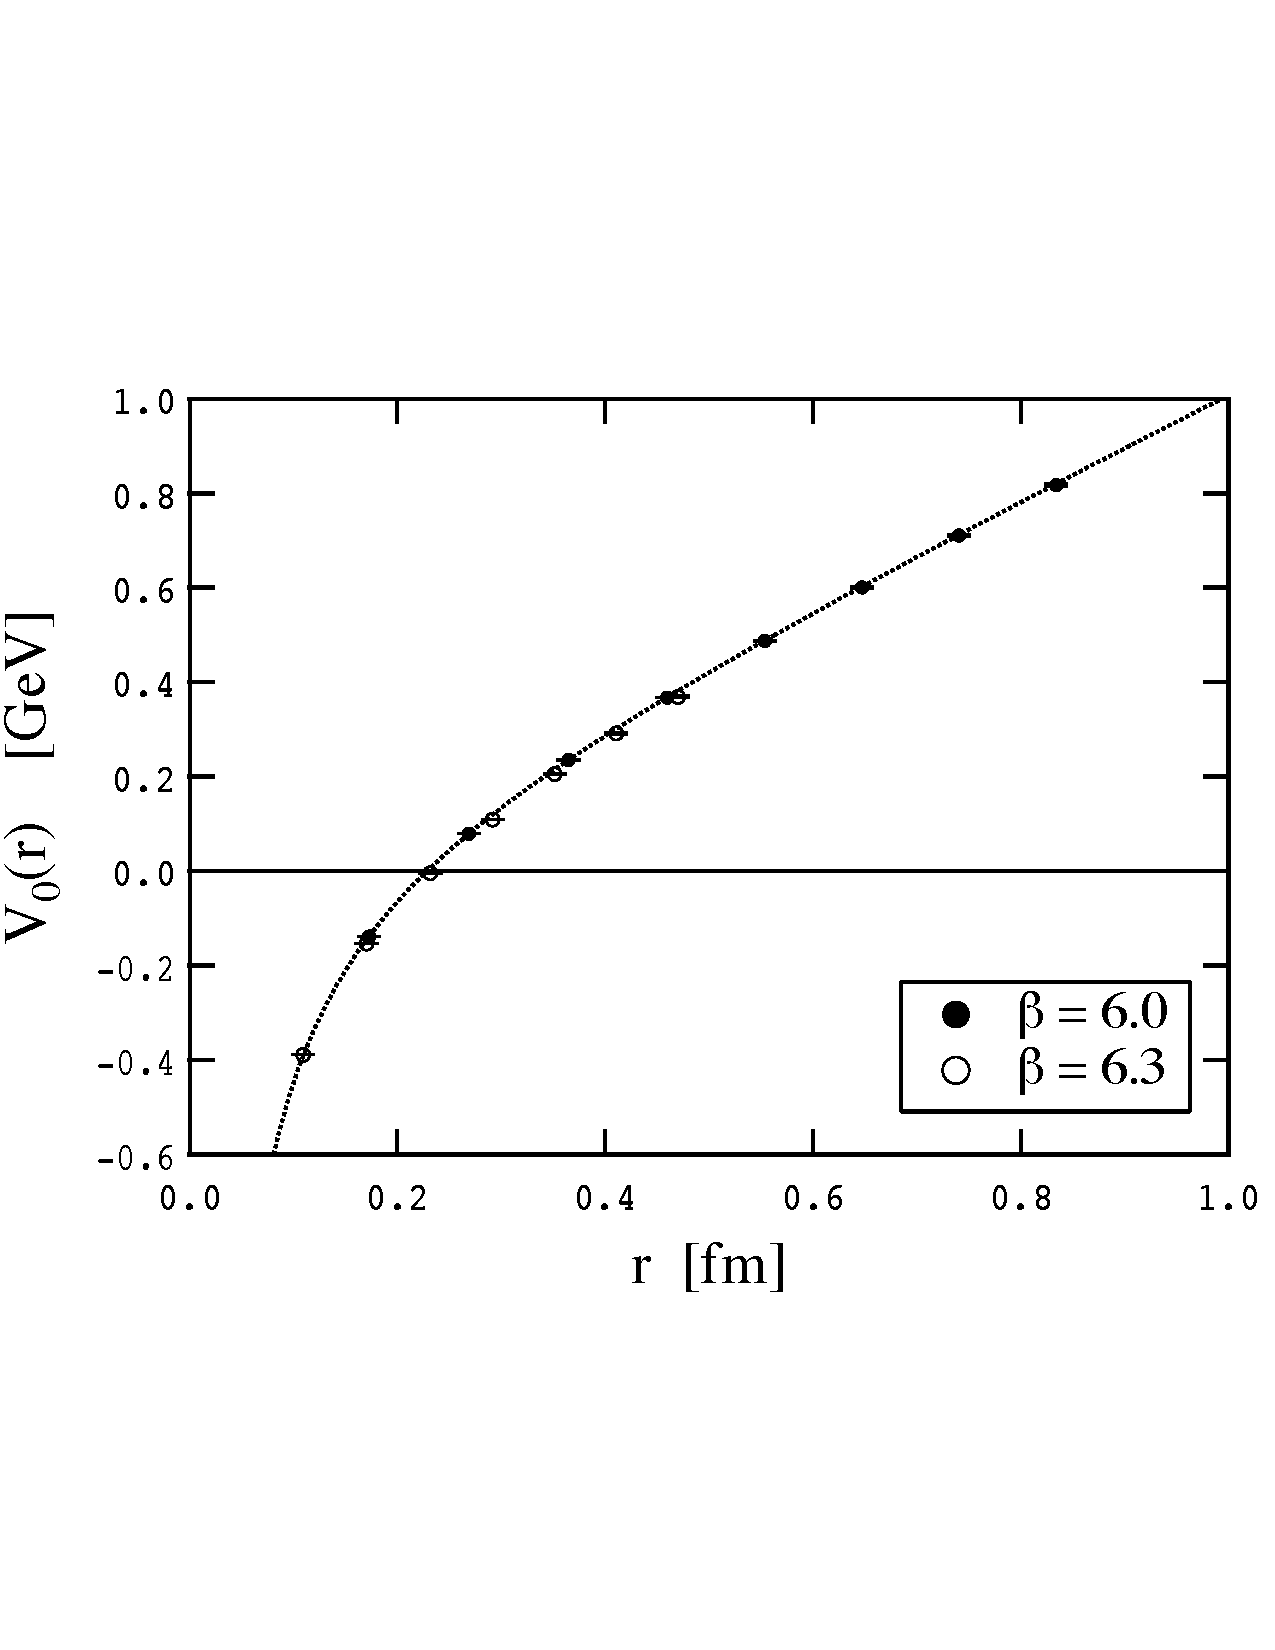
\includegraphics[width=0.4\textwidth]{figures/lattice_potential_qcd.pdf}
    \caption[Tracker material budget.]{
      The potential energy associated with two static quarks predicted by QCD as a function of distance, calculated numerically using the lattice technique.
      The potential increases roughly linearly with distance once a quark is no longer inside a hadron.
      The strong coupling used for the numerical calculation is denoted by $\beta$.
      Taken from \cite{lattice_potential}.}
    \label{fig:QCDpotential}
  \end{figure}  

  During a high energy collision involving a hadron like a proton, quarks and gluons are customarily ejected, and eventually reach a great enough distance to trigger the formation of new hadrons.
  But, the ejection is oftentimes so violent that even this new hadron fragments into new daughter hadrons, then these fragment, and so on.
  This fragmentation process produces a spray of hadrons, hadron decay products, and hadrons formed from QCD radiation analogous to bremsstrahlung, all traveling in approximately the same direction as the original ejected quark or gluon, which are collectively called a hadron jet.

  Unfortunately, while the production of jets is understood qualitatively, it is difficult to predict quantitatively due to yet another peculiar feature of QCD.
  The perturbative expansion described in the previous section is performed in powers of the interaction's coupling, with one factor of the coupling per vertex.
  In order for a truncated perturbation series to be a good approximation, the coupling must be significantly less than 1.
  Otherwise, diagrams with more vertices, representing higher order terms in the expansion, are in general more important than diagrams with fewer vertices, and no finite truncation can be accurate.
  Although the QCD coupling is less than 1 at high energy, making the perturbative approach still viable for very high energy collisions, the coupling explodes at low energies, which earns the strong interaction its name.
  Even at intermediate energies where QCD is technically perturbative, the number of diagrams that must be evaluated for an accurate result is still impractically large.

  \begin{figure}[h!]
    \centering
    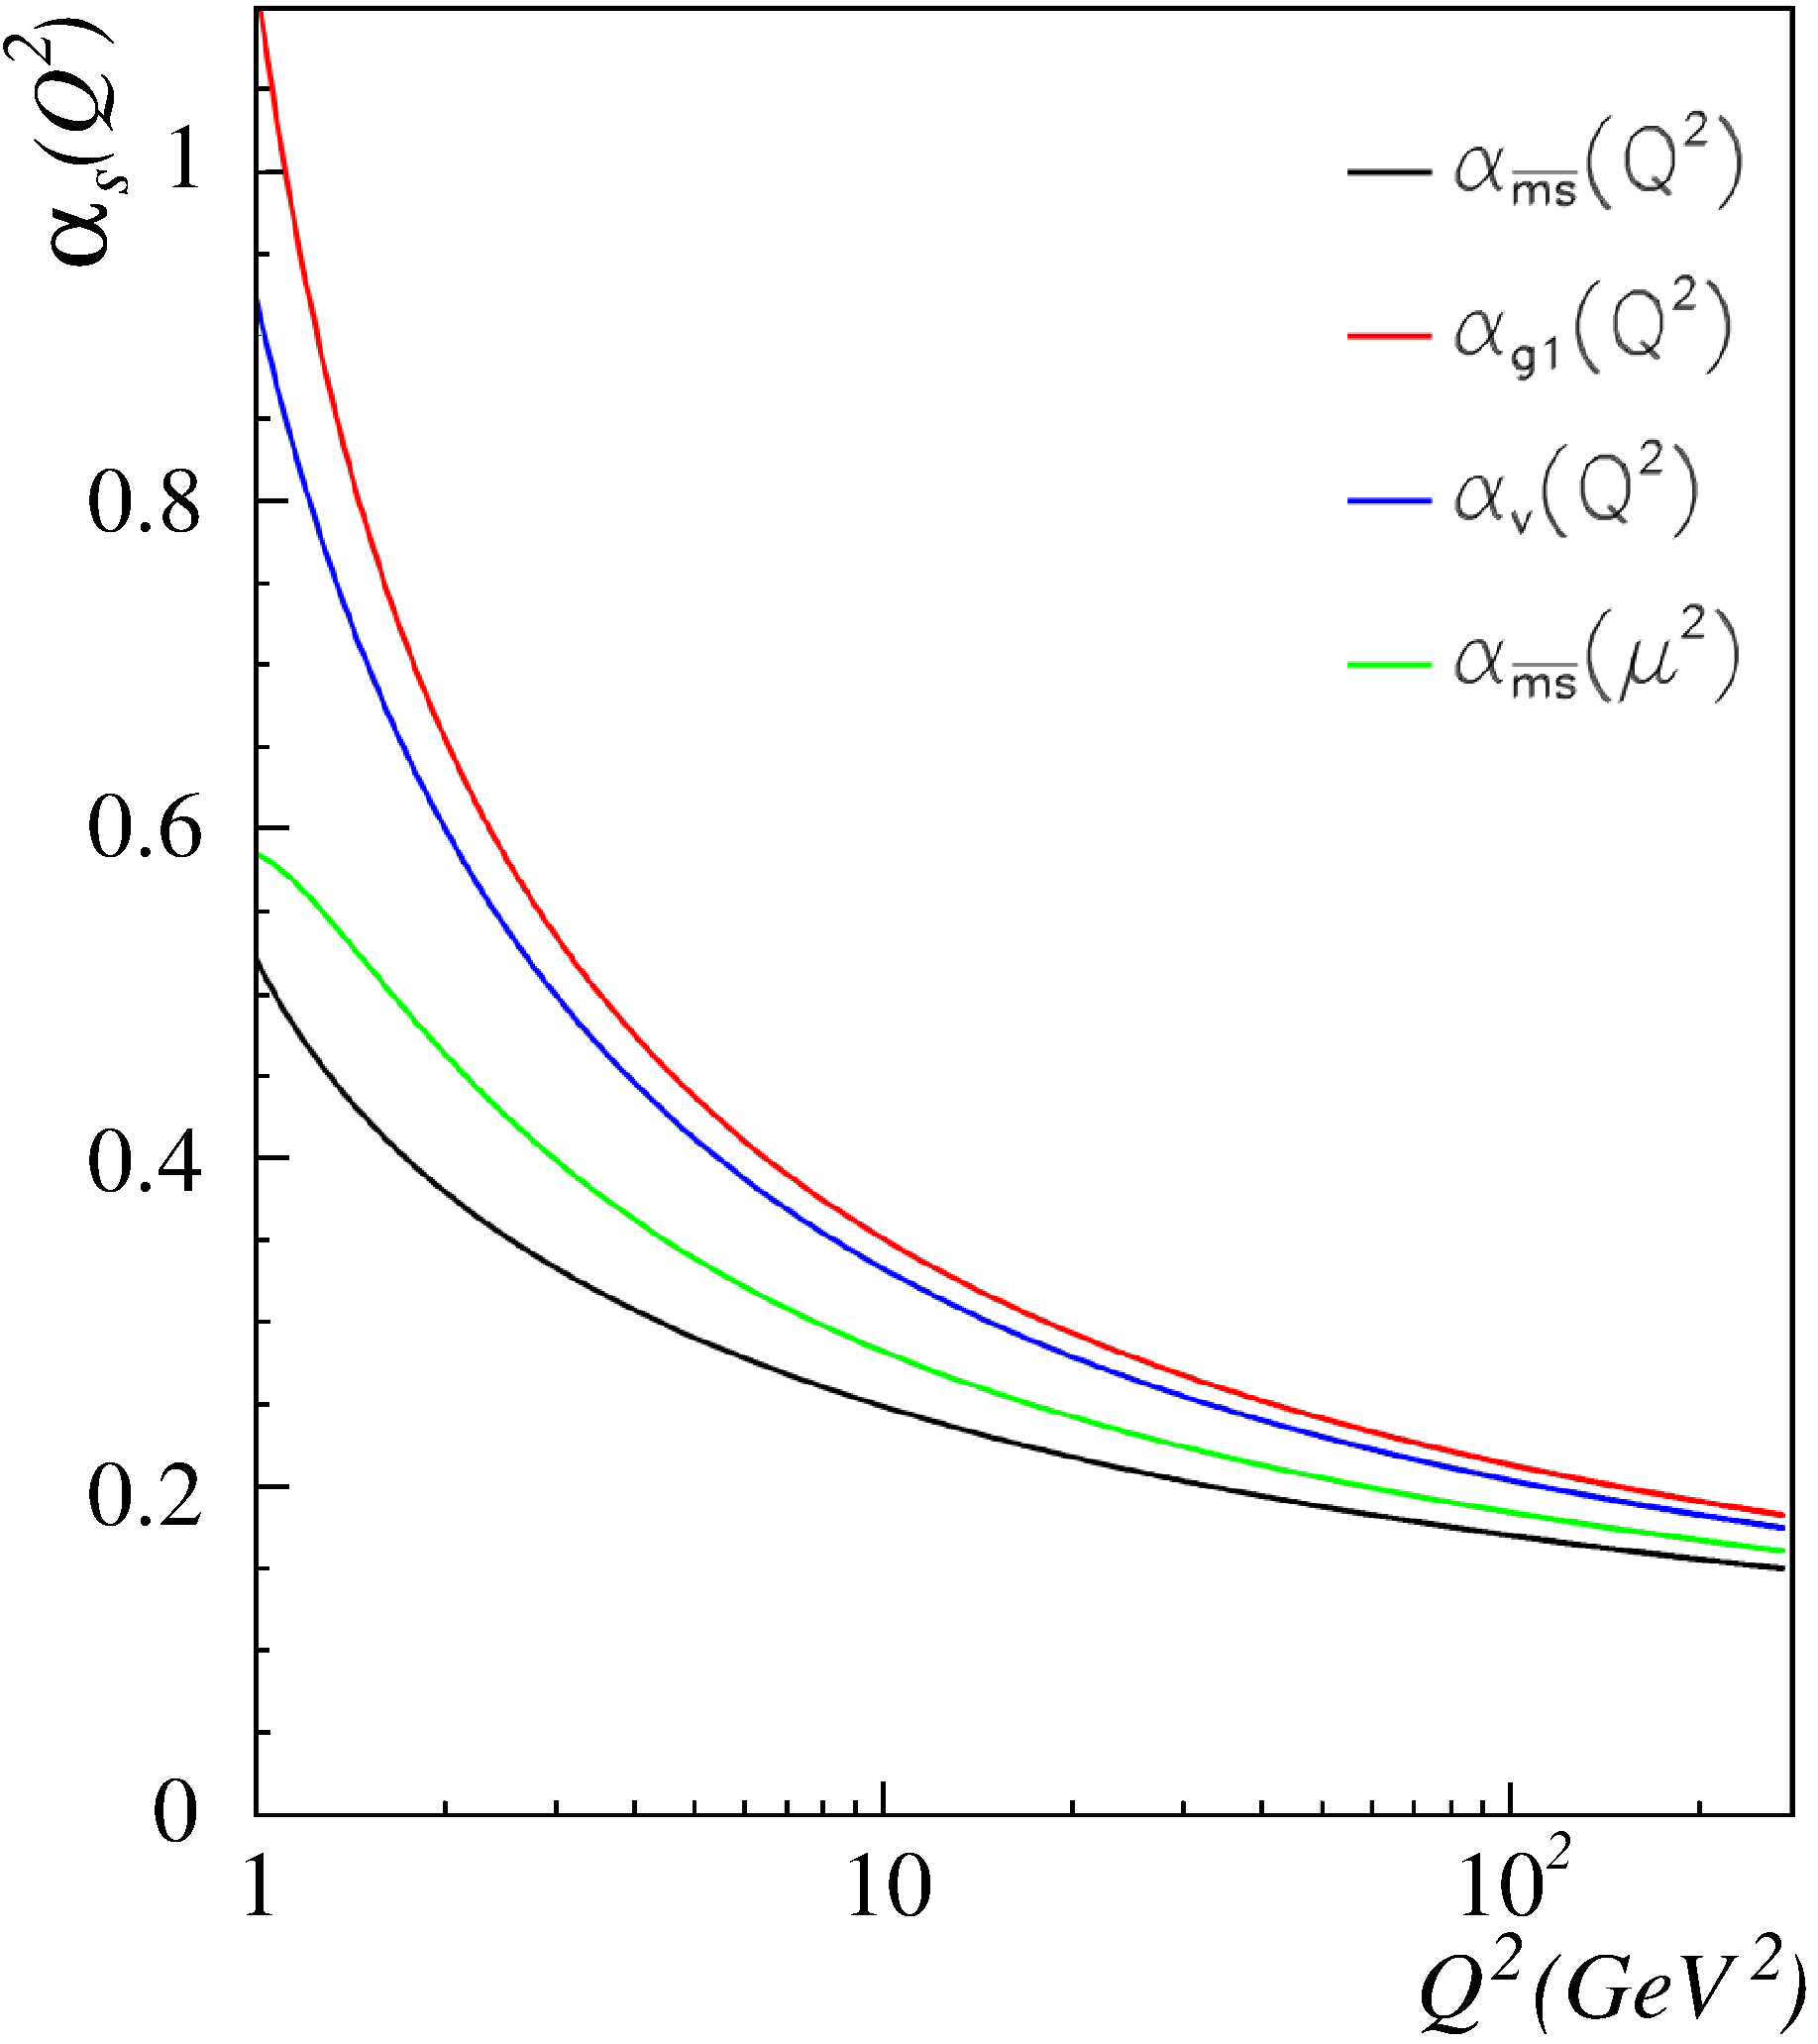
\includegraphics[width=0.4\textwidth]{figures/qcd_coupling.pdf}
    \caption[The QCD coupling as a function of the interaction energy.]{
      The QCD coupling explodes at low energy, making QCD non-perturbative for any interaction energy below around 1~GeV.
      The different lines are obtained for different methods of performing the calculation, specifically different renormalization schemes.
      Taken from \cite{qcd_coupling}.}
    \label{fig:QCDcoupling}
  \end{figure}  

  Non-perturbative approaches to QCD exist, including the lattice numerical method used to produce the plot shown in Figure~\ref{fig:QCDpotential}, but they are extremely computationally expensive for even the most simple calculations.
  It is not feasible to perform non-perturbative calculations of low energy QCD physics from first principles in an environment as complex as high energy hadron collisions.
  For the hadronization and fragmentation process, heuristic approximations tweaked to match data are used instead, typically the Lund String Model as implemented in the Pythia software package (see Section~\ref{sec:simulation}).
  Additionally, relatively low energy quarks and gluons can be emitted during the collision itself, called Initial State Radiation (ISR).
  A diagram of $u\bar{u} \rightarrow Z \rightarrow e^+e^-$ that includes a single ISR gluon is shown in Figure~\ref{fig:ISRdiag}.
  The most reliable way to predict ISR is to measure it in a very similar physics process, then convert this measurement to an expected rate in the physics process of interest.
  For example, ISR in $Z\rightarrow e^+e^-$ events is essentially identical to ISR in $Z\rightarrow \nu\nu$ events.
  
  \unitlength=2mm
  \begin{figure}[h!]
    \centering
    \begin{fmffile}{ISRdiag}
      \begin{fmfgraph*}(40,25)
        \fmfleft{i1,i2}
        \fmfright{o1,o2}
        \fmfbottom{b}
        \fmf{fermion,label=$u$,label.side=left}{i2,v1}
        \fmf{fermion,label=$\bar{u}$,label.side=left}{i1,vi}
        \fmf{fermion}{vi,v1}
        \fmf{gluon,label=ISR gluon,label.side=left}{vi,b}
        \fmf{photon,label=$Z$,label.side=left}{v1,v2}
        \fmf{fermion,label=$e^-$,label.side=left}{o2,v2}
        \fmf{fermion,label=$e^+$,label.side=left}{v2,o1}
      \end{fmfgraph*}
    \end{fmffile}

    \caption[A Feynman diagram including an ISR gluon.]{
      Initial State Radiation emitted as part of the hard collision, in this case $u\bar{u} \rightarrow Z \rightarrow e^+e^-$, can be at relatively low energy.
      This gluon will hadronize and add a jet to the event.
      QCD ISR is difficult to predict accurately due to the intractability of QCD at low energy.
    }
    \label{fig:ISRdiag}
  \end{figure}  
  \unitlength=2mm

  In summary, QCD's intractability at low energy combined with its raw strength make precise predictions of the outcome of hadron collisions difficult to obtain, despite the Standard Model's overall success in describing the interactions of elementary particles.
  The Standard Model prediction cannot always be obtained directly from first principles with satisfactory accuracy.

  \subsection{Parton Distribution Functions} \label{sec:PDFs}

  Being composite particles bound by QCD, the internal structure of hadrons is rich and difficult to understand quantitatively, due to the impossibility of using perturbation theory at the low energies that prevail in hadrons.
  Of greatest interest is the internal structure of the proton, the only stable hadron.

  The proton is often said to be a bound state of two up quarks and one down quark.
  This is true enough---the {\it net} composition of a proton is two up quarks and one down quark---but is an oversimplification.
  The quarks in a proton constantly emit and absorb gluons, which can split to quark-antiquark pairs, which can in turn annihilate back to gluons.
  Viewed at a small enough length scale, the proton is not a simple object, and not even a bound state of 3 quarks, but rather a complex cloud of quarks and gluons with various energies.
  This is problematic for any attempt to predict the outcome of proton collisions, because one cannot be sure which of these subcomponents, called partons, will be the component of the proton that actually experiences a collision.
  Due to the intractability of QCD at low energy, the composition of a proton is known only from a fit to data, and called a Parton Distribution Function (PDF).
  PDFs are typically expressed as the probability to find a parton of a given species carrying a given fraction of the proton's energy, as shown in Figure~\ref{fig:PDF}.
  These PDFs display a few sensible features described in the figure's caption.
  A large number of proton collisions collectively sample all the possible initial partons, with momentum distributions described by the PDFs.
  Thus, a dataset composed of proton collisions naturally probes a wide range of collision energies with a variety of colliding particles, making proton collisions well-suited to searches for new particles of unknown properties.

  \begin{figure}[h!]
    \centering
    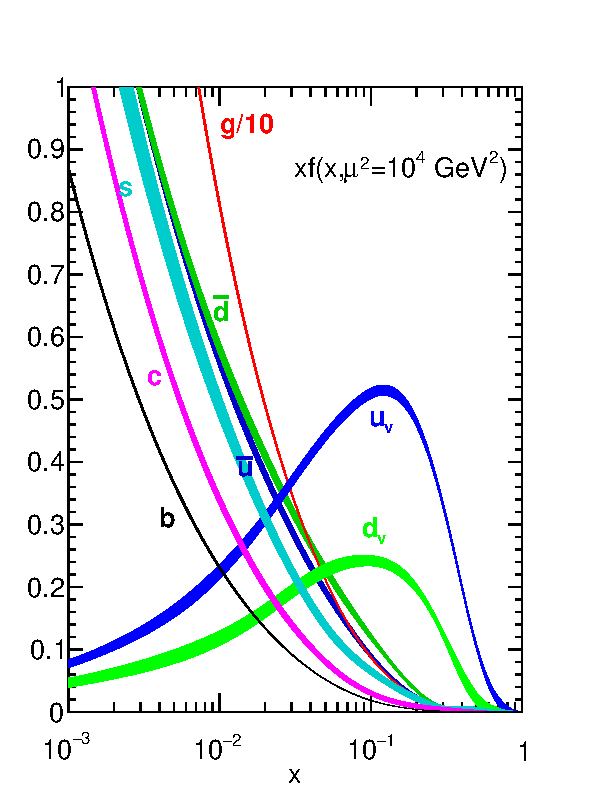
\includegraphics[width=0.4\textwidth]{figures/parton_distribution_function.pdf}
    \caption[Proton parton distribution function.]{
      The plot shows the measured parton distribution function for a proton at an interaction energy of 100~GeV.
      The horizontal axis $x$ is the fraction of the proton's total momentum, and the vertical axis is the probability distribution.
      The finite thickness of the curves indicates the uncertainty.
      As expected for a proton, $uud$, the probability to collide with an up quark is around twice the probability to collide with a down quark at any energy.
      The $v$ subscript on these two curves indicate that these are the ``valence'' quarks, the only quarks that are present as more than transient products of gluon splitting.
      It is much less likely to find an up or down antiquark, and roughly equally likely to find either, because these antiquarks are produced only by gluons splitting to quark-antiquark pairs.
      Since they are also produced only transiently by gluon splitting, the probability to find a heavier quark, namely $s$, $c$, or $b$, is exactly equal to the probability to find a heavy antiquark.
      Since the heavy quark and antiquark curves overlap, only the quark curves and represent both.
      Quarks aside, notice that the gluon curve (red) has been suppressed by a factor of 10 to fit on the plot.
      To a decent approximation, high energy proton colliders in practice collide gluons.
      Taken from \cite{PDFs}.}
    \label{fig:PDF}
  \end{figure}  


\section{Some Problems with the Standard Model} \label{sec:SMproblems}

The Standard Model is extremely successful, as epitomized by the result in Table~\ref{tab:electronmu}, but not entirely satisfactory.
In fact, its success in laboratory experiments is a source of frustration for elementary particle physicists, as there are precious few hints as to how its deficiencies can be repaired.
This section introduces a few of the known problems with the Standard Model.

  \subsection{Gravity, and the Standard Model as an Effective Field Theory} \label{sec:gravity}

  In Section~\ref{sec:standardmodel}, there is never any mention of gravity as an interaction between particles.
  This is because the Standard Model entirely omits gravity from its description of nature, which means the Standard Model cannot possibly be the final theory.
  Instead, the Standard Model must be only an {\it effective theory}, a low energy approximation of nature that must be replaced by a more fundamental theory at some cutoff energy.
  In the case of the Standard Model, this cutoff cannot be any larger than the energy at which gravity becomes relevant in the interactions of elementary particles, called the Planck scale.

  Unlike the fields of the Standard Model, whose couplings are dimensionless, the gravitational coupling $G$ has dimensions of inverse energy squared.
  An effective field theory of the weak interactions developed by Enrico Fermi, which models the weak interactions of fermions without mediating bosons, has a similar coupling, $G_F \approx \frac{1}{(100\mathrm{~GeV})^2}$.
  The energy scale embedded in the coupling is a message from nature, hinting that this effective theory must be replaced by something more fundamental in order to model physics at the scale of around 100~GeV or more.
  Nowadays, we recognize this energy as the mass scale of the weak interaction's mediating bosons.
  At interaction energies on the order of 100~GeV or larger, there is enough energy to produce the boson itself as a resonant excitation of the field, a real particle, and the underlying theory is revealed.
  Making an analogous inference from the gravitational coupling, one obtains the maximum possible cutoff energy for the Standard Model, the Planck energy of around $10^{19}$~GeV, at which gravity must be incorporated into the quantum theory.

  Moreover, the Standard Model becomes self-inconsistent at very high energies, even ignoring the gravity problem \cite{landaupole,higgstriviality}.
  The couplings of both electromagnetism and of the Higgs to itself increase with increasing energy, until eventually diverging at very high energy scales, a theoretical consistency issue called quantum triviality.
  As a result, the Standard Model's formulation of electromagnetism cannot be used for any energy greater than around $10^{34}$~GeV~\cite{landaupole}.
  Although this energy is far greater than the Planck energy, at which the Standard Model must fail anyway due to its exclusion of gravity, it is a completely independent indication that the Standard Model must be only a low energy limit of some more fundamental theory that supersedes it at high energy, one that does not exhibit these kinds of problems.
  Even if one supposes that gravity's exclusion from the Standard Model is not actually a problem, that attempting to treat gravity like the other interactions is misguided, the Standard Model still cannot be the final theory.

  The Higgs self-interaction similarly diverges above the Planck scale, although had the Higgs mass turned out to be only around 200~GeV rather than the measured 125~GeV, the problem would arise below the Planck scale, and a Higgs mass as small as around 600~GeV would have made the triviality scale only a few TeV, accessible to current experiments \cite{higgstriviality}.

  Thus, there exist known finite energy scales at which the Standard Model {\it must} fail, due both to its exclusion of gravity and to internal mathematical consistency issues, and the actual cutoff energy may be much smaller than these upper limits.
  Every experiment probing an unexplored energy scale has a chance to be the first to observe a hint as to what this more fundamental theory looks like.

  \subsection{The Hierarchy Problem} \label{sec:hierarchy}

  As described in the previous section, the energy scales of the weak interaction and of gravity differ by approximately 17 orders of magnitude.
  If the Standard Model emerges from some more fundamental theory at the Planck energy, then what effect has pushed the weak scale down 17 orders of magnitude?
  The most troublesome expression of this apparently inexplicable hierarchy of energy scales centers on the mass of the Higgs boson.
  In the Standard Model, the Higgs mass $m_h$ is given approximately by \cite{SUSYnaturalness,higgsmass},
  \begin{equation} \label{eqn:higgsmass}
    m_h^2 \approx 2\mu^2 + (\Delta m_h)^2
  \end{equation}
  where $\mu$ is a free parameter called the bare mass of the Higgs that would most naturally be 0, and $\Delta m_h$ is an adjustment that the Higgs acquires via its interactions with other fields in the Standard Model,
  \begin{equation} \label{eqn:masscorrection}
    \Delta m_h^2 \approx \frac{3}{4\pi^2}\left(\lambda^2 - \lambda_t^2 + \ldots\right)\Lambda^2
  \end{equation}
  where $\lambda$ is the Higgs' coupling to itself, $\lambda_t$ is its coupling to the top quark, and $\Lambda$ is the energy at which the Standard Model is replaced by a more fundamental theory that is assumed not to contribute any further corrections to the Higgs mass, at most the Planck Energy.
  The couplings of the Higgs to all the fermions of the Standard Model appear in the correction with the same form as the top's $\lambda_t$, but the coupling of the top quark is by far the most important, since at $\sim$1 it is by far the largest, as can be seen from the mass column in Table~\ref{tab:fermions}.
  The Higgs' self-coupling is somewhat smaller \cite{higgsmass}.
  Therefore, $\Delta m_h^2 \sim -\Lambda^2$.
  If one takes $\Lambda \approx 10^{19}$~GeV, the Planck Energy, then Equation~\ref{eqn:higgsmass} is deeply implausible after also inserting the experimental value $m_h \approx 125$~GeV,
  \begin{equation}
    (125)^2 \approx 2\mu^2 - (10^{19})^2.
  \end{equation}
  The Higgs mass of 125~GeV emerges from almost perfect cancellation of two terms with values around $10^{19}$~GeV.
  A model that produces an output of a very different order of magnitude from the generating input is said to be finely tuned.
  The Standard Model, epitomized by the Higgs mass, is {\it egregiously} finely tuned.
  This is the Hierarchy Problem.

  Of course, the Standard Model's cutoff need not be the Planck Energy. 
  If $\Lambda$ is only 1000~GeV, then the Hierarchy Problem as stated disappears, and one can expect to discover new physics in elementary particle interactions at this experimentally accessible scale.
  Still, merely not being the Standard Model is insufficient; the replacement theory also needs to introduce a mechanism to stabilize the Higgs mass, lest it make its own contributions or allow the Standard Model fields to continue pushing it to large values.
  By far the most popular proposal for the kind of model that may supersede the Standard Model at the TeV scale is called Supersymmetry, discussed in Section~\ref{sec:SUSY}.

  \subsection{Massive Neutrinos} \label{sec:neutrinomasses}

  In the Standard Model, all fundamental particles acquire mass through their interactions with the Higgs, and the neutrinos are strictly massless.
  However, recent measurements of neutrinos have established that they undergo flavor oscillation, whether produced by cosmic rays in the atmosphere \cite{atmospheric_neutrinos}, or by nuclear processes in reactors on Earth \cite{reactor_neutrinos} or in the Sun's core \cite{solar_neutrinos}.
  This means that, just as for quarks, the neutrino mass eigenstates are not equal to the interaction eigenstates, and more importantly that the neutrinos' mass eigenstates are not equal {\it to each other} \cite{nufit}.
  This is only possible, of course, if at least 2 of the 3 neutrinos are massive.
  Although difficult particles to measure, experiments have managed to map out the neutrino mixing matrix analogous to the CKM matrix for quarks, the Pontecorvo-Maki-Nakagawa-Sakata matrix \cite{pdg},
  \begin{equation}
    U_{PMNS}
\approx
    \begin{bmatrix} 
      0.800 \leftrightarrow 0.844 & 0.515 \leftrightarrow 0.581 & 0.139 \leftrightarrow 0.155 \\
      0.229 \leftrightarrow 0.516 & 0.438 \leftrightarrow 0.699 & 0.614 \leftrightarrow 0.790 \\
      0.249 \leftrightarrow 0.528 & 0.462 \leftrightarrow 0.715 & 0.595 \leftrightarrow 0.776 
    \end{bmatrix}
  \end{equation}
  where each element of the matrix shows the range consistent with experiment.
  Mysteriously, $U_{PMNS}$ is not approximately diagonal, unlike the CKM matrix.
  Nonzero neutrino masses are entirely inconsistent with the Standard Model and, to date, are the only observables measured in laboratories that the Standard Model has failed to predict accurately.

  \subsection{Astrophysical Evidence of Dark Matter} \label{sec:DMevidence}

  Over the last century, astrophysical observations have assembled conclusive evidence that most of the Universe's gravitating mass has at most a neutrino-like interaction cross section.

  Some of the oldest evidence was obtained from galactic rotation curves.
  In general, stars far from the cores of galaxies have much greater orbital velocity than would be inferred from the visible mass to their interior, implying either that general relativity is not a good model of gravity on large distance scales, or that most of the gravitating mass in galaxies is weakly interacting and arranged as an extended halo \cite{rotationcurves}.
  Recent observations have concluded with good precision that this is true also in the Milky Way \cite{rotationcurves_MW}.

  Observation of the Cosmic Microwave Background (CMB) has allowed for measurement of the Universe's energy density, and the forms taken by that energy density.
  The best fit is a Universe composed of about 6 times as much ``dark'' matter as visible matter, consistent with the ratio that would explain galactic rotation curves \cite{planckCMB}.
  No modification of gravity has ever been found that can satisfactorily explain both the rotation curve observations, and explain these energy density measurements.

  Observations of the Universe at more recent times have found a few cases of colliding galaxy clusters, most famously the Bullet Cluster, that offer further evidence for the existence of dark matter.
  In galaxy cluster collisions, the luminous matter can collide and produce a very hot plasma due to its relatively strong interactions, while dark matter continues on unaffected.
  The luminous matter can be accounted for directly via the emissions of the hot plasma, while the location of the mass, visible or not, can be measured by observing the gravitational lensing of the light of more distant galaxies by the foreground colliding clusters \cite{bulletcluster}.
  The result of this analysis for the Bullet Cluster is shown in Figure~\ref{fig:bulletcluster}.
  The visible matter, revealed by its x-ray emissions, is caught in the collision zone at the center, while the majority of the gravitating matter has continued on unaffected, and is detectable only through its powerful gravitational lensing on either side of the luminous plasma.
  The inferred ratio of dark matter and visible matter is consistent with the amount that would explain both rotation curves and the energy densities measured using the CMB.
  Again, no modification to gravity has been found that can simultaneously explain galactic rotation curves and the energy density measurements from the CMB, and also the gravitational lensing observed in the Bullet Cluster and similar collisions.
  \begin{figure}[h!]
    \centering
    \includegraphics[width=0.4\textwidth]{figures/bulletcluster.pdf}
    \caption[Mass and x-ray distributions of the Bullet Cluster.]{
      The distribution of luminous matter emitting x-rays (black dots) and the location of mass inferred through gravitational lensing of background sources (contours) are offset.
      The plasma emitting x-rays has been slowed and shocked as a result of the astronomically recent collision between the galaxy clusters, and so has been left behind by the dark matter, which constitutes most of the mass and was unaffected by the collision due to its negligible interaction cross section.
      Taken from \cite{bulletcluster}.}
    \label{fig:bulletcluster}
  \end{figure}  

  Finally, astronomers have recently identified a few small galaxies that appear to contain little or no dark matter \cite{zeroDMgalaxy}.
  While this is an extraordinarily rare occurrence and effectively impossible in a large galaxy like the Milky Way, small galaxies are subject to larger statistical fluctuations, and the Universe has a rather large sample size of galaxies.
  It is difficult to imagine a modification of gravity that could, in most observations, cause there to appear to be around 6 times are much invisible mass in the Universe as visible mass, but in some small galaxies appear as if there is no modification at all.

  If dark matter is not composed of a weakly interacting particle beyond the Standard Model, the only remaining possibility is that it is composed of larger non-radiating masses like rogue planets or black holes produced in the high-density primordial Universe and surviving to the present day.
  This possibility is taken seriously, and can be investigated by searching for small microlensing events, where the light of a distant star is briefly gravitationally lensed when one of these bodies passes between an Earth-based telescope and the star.
  As there is around 6 times as much dark mass as visible in the galaxy, such an event should be relatively common.
  No excess of such events is observed in microlensing and complementary searches, so that if all dark matter has exactly the same mass, it cannot have any mass in the range $10^{-7}M_{\mathrm{Sun}} < M_{DM} < 10^5 M_{\mathrm{Sun}}$ \cite{primordialBH_dist}.
  This leaves open the possibility that dark matter could be composed of black holes of small mass, with Schwarzschild radius around 0.1~mm or less, or that it could be composed of bodies with a range of masses.
  However, both possibilities are disfavored.
  It is suspected that small primordial black holes would generically be captured by stars, eventually migrate to the core as the star dies, and destroy the compact remnant via accretion \cite{primordialBH}, but no such events are observed.
  As for the latter possibility, the data places such strong constraints on the acceptable mass distribution that it is necessary to construct one carefully by hand to avoid the limits \cite{primordialBH_dist}.
  Particle dark matter, despite its own history of non-observation, remains the possibility most easily reconciled with the data.

  There is especially strong hope for detecting particle dark matter at the TeV scale, due to a suggestive coincidence called the Weakly Interacting Massive Particle (WIMP) Miracle.
  The characteristic energy scale of the weak interaction is $\sim100$~GeV.
  A hypothetical particle with mass in the suitable range, on the order of 1 to 10,000 GeV, interacting via the Standard Model's weak interaction or a similar interaction, would have been produced in the early Universe and survived to the present day at the proper density to account for the observed cold dark matter \cite{WIMPmiracle}.
  Furthermore, it would be an astonishing coincidence if the dark matter particle is only distantly related to the Standard Model, perhaps only by gravitational interactions, and yet somehow by dumb luck ended up with a relic mass density on the same order of magnitude as that of the Standard Model particles.
  Viewed in light of indications that new physics ought to be found at the TeV scale from the Hierarchy Problem and other issues with the Standard Model, the case for particle dark matter at the TeV scale is compelling.
  The chief argument against WIMPs is that they have not yet been observed in experiments despite concentrated efforts, yet much of the parameter space remains untouched.
  It is a high priority of current experiments to extend sensitivity into these regions.

\section{Supersymmetry} \label{sec:SUSY}

Among all the proposals for extending the Standard Model and repairing many of its issues at the TeV scale, supersymmetric extensions are by far the most popular and intensively researched.
Supersymmetry proposes that for every Standard Model fermion (boson), there exists a {\it superpartner} boson (fermion) with nearly identical properties aside from its spin.
The superpartners of spin-$\frac{1}{2}$ particles are spin-0, and the superpartners of spin-1 and spin-0 particles are spin-$\frac{1}{2}$.
For example, the superpartner of the electron is a spin-0 particle called the scalar electron, usually contracted to ``selectron.''
The fermionic superpartners of bosons instead receive the ``-ino'' suffix, for example ``higgsino.''
If supersymmetry is realized at the TeV scale, it would resolve many of the Standard Model's problems, and would be experimentally testable using TeV-scale particle colliders.
This section introduces some of the theoretical reasons for the popularity of supersymmetry, and how it may be targeted experimentally.

  \subsection{Theoretical Appeal} \label{sec:SUSYappeal}

  A full discussion of the theoretical appeal of supersymmetry is beyond the scope of this thesis, so this section briefly discusses only a pair of the most compelling points that are most closely connected to why supersymmetry at the TeV scale is of great interest.
  First, supersymmetry provides a well-motivated dark matter candidate, a concrete realization of the WIMP Miracle.
  Second, it resolves the Hierarchy Problem and is almost certainly the only solution that possibly can; if supersymmetry is not realized at the TeV scale, it likely means that the Standard Model's fine tuning has somehow been misinterpreted and is not in fact a problem.

  Supersymmetry's dark matter candidate arises as a side effect of a solution to an unrelated problem.
  Naive implementations of supersymmetry make possible the decay $p \rightarrow \pi^0~e^+$ via mediation by a squark (the pion is the lightest meson and the only hadron lighter than the proton).
  The proton would be highly unstable for any reasonable squark mass, in conflict with the lower limit on this decay mode of some $10^{32}$ years, and the any-mode limit of more than $10^{29}$ years \cite{pdg}.
  However, it is possible to have a stable proton within supersymmetric models, by proposing that there exists a conserved multiplicative quantum number called R-parity and assigning superpartners odd R-parity and Standard Model particles even R-parity.
  This saves the proton, but as a side effect also makes the lightest supersymmetric particle (LSP) stable, since decays to final states including other superpartners are kinematically impossible and decays to final states containing only Standard Model particles cannot conserve R-parity \cite{pdg}.

  At first, LSP stability appears to be a problem as severe as proton decay.
  If the LSP is stable, then there should be a large relic population persisting from the primordial plasma, indeed this relic population may represent the majority of the mass of the Universe, but no such population has ever been observed.
  However, astrophysical observations have assembled a compelling case that a majority of the mass of the Universe is not of the Standard Model, making it possible that stable LSPs {\it have} been observed, as dark matter, via their gravitational interactions.
  Of course, this position is only tenable if one of the superpartners has the properties necessary to be a dark matter candidate.
  The superpartners of neutrinos, the sneutrinos, are an obvious first guess, but their interaction cross sections are too large in generic implementations of supersymmetry, so that a sneutrino LSP requires a special purpose-built model to be viable \cite{sneutrinos}.
  Fortunately, the neutral superpartners of the weak bosons, the neutralinos, could have even smaller interaction cross sections than sneutrinos, and are ideal dark matter candidates.
  Moreover, as part of supersymmetry's solution to the Hierarchy Problem, the neutralinos in general and especially the higgsino are constrained to be relatively light \cite{distracksAMSB, SUSYnaturalness, naturalWIMP}, making a neutralino LSP plausible on more than phenomenological grounds.

  The supersymmetric solution to the Hierarchy Problem is founded on a simple observation.
  In Equation~\ref{eqn:masscorrection}, the Higgs' coupling to itself, a boson, and to the top quark, a fermion, appear with opposite signs.
  This is general: the contributions of bosons and of fermions to the Higgs mass have opposite signs.
  Among the Standard Model fields, this is not very helpful, since the top quark simply dominates the other fields.
  But, if every boson had a fermion counterpart with exactly the same properties and vice versa, all contributions to Equation~\ref{eqn:masscorrection} would exactly cancel.
  Of course, experiments have long excluded the existence of, say, a selectron of the same mass and interactions as the electron, so supersymmetry must be spontaneously broken if it exists, with the superpartners pushed to a higher mass scale.
  A variety of well-motivated mechanisms for this have been proposed \cite{GMSB_theory,distracksAMSB}.
  Whatever the mechanism, the scale of supersymmetry breaking would lead directly to the observed Higgs mass, implying that superpartners and especially the higgsino should begin to appear at energies not far beyond the observed Higgs mass \cite{distracksAMSB,GMSB_theory,SUSYnaturalness,naturalWIMP}.

  \subsection{Experimental Signatures} \label{sec:SUSYexp}

  Since every supersymmetric particle must decay to the nearly undetectable LSP, the primary signature of superpartner production in colliders is large missing energy and momentum, carried away by the undetectable LSP.
  Additionally, conservation of R-parity requires that superpartners be produced in pairs, so that these events are characterized by {\it two} heavy invisible particles.
  As experimental constraints on the visible superpartner masses increase, the likelihood that the decays are extremely energetic also increases.
  Two particles with large masses of perhaps 2~TeV would be produced only rarely in state of the art accelerators, but their events would be extraordinarily high energy, unless the LSP mass is also large and absorbs most of the decay energy.

  By definition, the LSP is the most energetically accessible superpartner.
  Even so, the preferred supersymmetry search strategy is to use the invisibility of the LSP to identify decay chains of more massive but more strongly interacting superpartners, as the LSP itself must  have a very low production rate due to its weak interaction cross section, if it exists.
  At hadron colliders, the best candidate superpartners are those participating in the strong interactions, squarks and gluinos, due to the relatively large production cross sections for strongly interacting particles (see Figure~\ref{fig:SUSYxsec}). 
  Unfortunately, while the mass of the LSP is restricted to a relatively low value if supersymmetry is to solve the Hierarchy Problem, the masses of other superpartners are not as strongly constrained.
  Attempts to observe the LSP in decays of more easily produced superpartners require that these intermediate states have accessible masses, which is not necessarily the case for any experiment to date \cite{SUSYnaturalness,naturalWIMP}.
  It may be necessary to search for direct LSP production if the other superpartners are too massive, which will require a vast dataset due to the low production rate.
  As the present datasets are still too small for highly sensitive direct LSP searches, most current analyses are two-dimensional, targeting a relatively easily pair-produced heavy superpartner and the LSP ultimately produced at the end of its decay chain.

  In some supersymmetric models, a relatively large supersymmetry energy scale tends to suppress the mass splitting of the lightest chargino \chionepm and lightest neutralino \lsp, for instance in the model described in \cite{distracksAMSB},
  \begin{equation}
    \frac{\Delta m}{m} \sim \left(\frac{m_W}{\mu}\right)^4
  \end{equation}
  where $\frac{\Delta m}{m}$ is the fractional splitting of the nearly-degenerate \chionepm and \lsp masses and $\mu$ is a parameter appearing in the supersymmetric Higgs potential, which is partially responsible for setting the mass scale of superpartners.
  A $\mu$ value of a few hundred GeV would produce a mass splitting of one part per thousand or less, as small as a few hundred MeV.
  As the viable masses of superpartners are pushed to larger values by experimental constraints, such a scenario becomes increasingly plausible.
  At a splitting of a few hundred MeV, the phase space of the decay $\chionepm \rightarrow \pi^{\pm} \lsp$ is so small that the lifetime becomes sufficient to produce macroscopic decay lengths.
  Furthermore, with only a few hundred MeV available to the pion, it would fall below the minimum \pt for track reconstruction, making the decay of \chionepm completely invisible.
  As \chionepm has a macroscopic decay length and nonzero electric charge, this invisible decay can produce the remarkable experimental signature called a disappearing track.
  Interest in this long-lived \chionepm model and other models that include long-lived particles has recently grown, motivated in part by the growing theoretical plausibility, and in part by the additional sensitivity that exploitation of long-lived particle signatures can provide.
  The disappearing track signature in particular is used by the search in Section~\ref{sec:distracks}.

  \subsection{Simplified Models} \label{sec:SUSYsms}

  Due to the large number of particles and free parameters in even the simplest supersymmetric extensions of the Standard Model, it is not possible to make exact calculations that hold for every possible realization of supersymmetry, and every supersymmetry simulation is to some extent dependent on the exact choices of free parameters.
  To make calculations tractable, the community has widely adopted use of simplified models \cite{SMS}.
  Simplified models are effective field theories that assume all superpartners except those of interest are at an inaccessible mass scale.
  Effectively, instead of extending the Standard Model with every superpartner simultaneously, only a few particles, perhaps only the gluino and the LSP, are added.
  This makes it possible to calculate pair-production cross sections as a function of mass, allows for the decay channel(s) to be set without worrying about the model's self-consistency, and so on without excessive computational effort.
  The gluino pair-production cross section as a function of mass in such a simplified model is shown in Figure~\ref{fig:SUSYxsec}.
  \begin{figure}[h!]
    \centering
    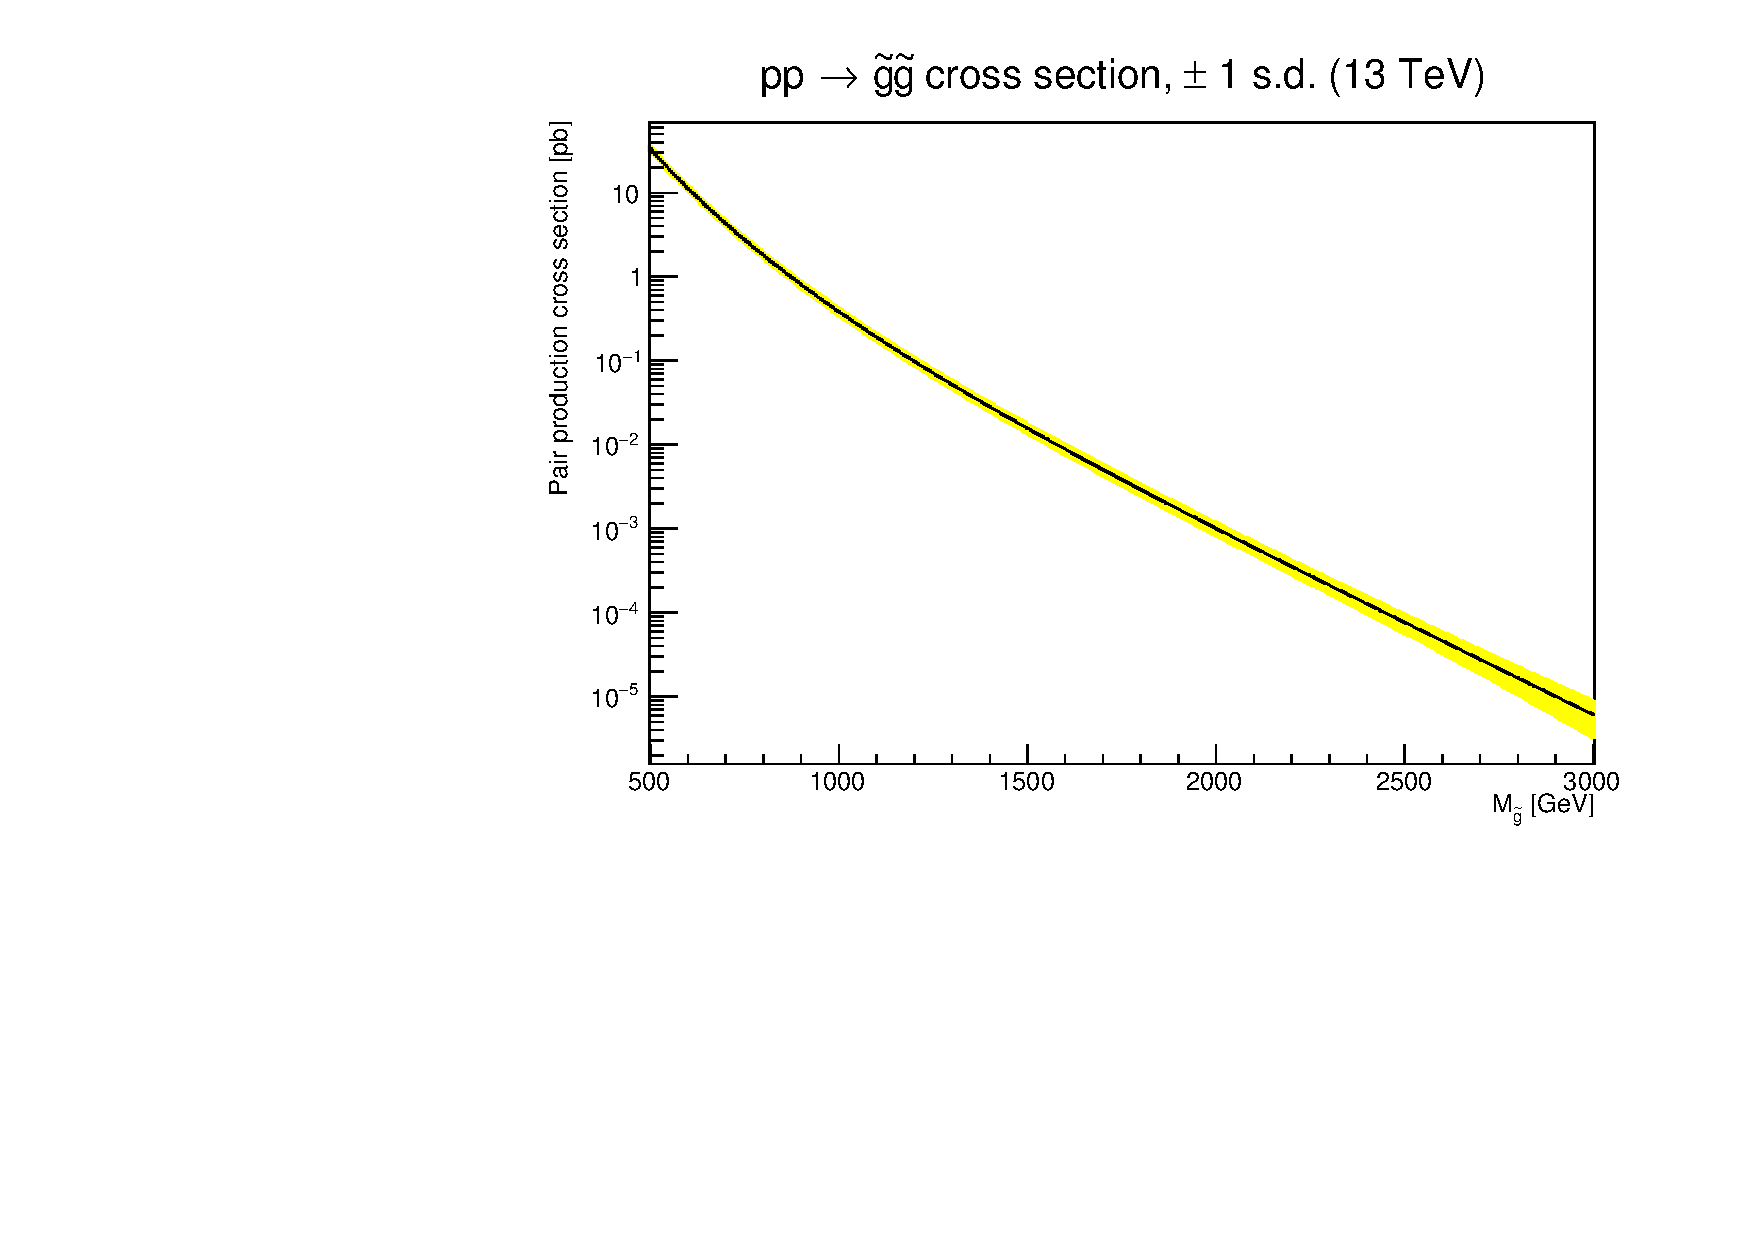
\includegraphics[width=0.85\textwidth]{figures/gluino_xsec.pdf}
    \caption[Theoretical gluino pair production cross section in simplified models.]{In simplified models, it is possible to calculate superpartner production cross sections from theory.
Here, the theoretical gluino pair production cross section in 13 TeV proton-proton collisions is shown in black, with the one standard deviation uncertainty shown as a yellow band.
The cross section drops rapidly with increasing mass.
Based on cross section values used in \cite{MT2_2019}, calculated in \cite{SUSYxsecs}.
Compare Figure 5 (upper) from \cite{SUSYxsecs}, of which this is a simplified reproduction.
}
    \label{fig:SUSYxsec}
  \end{figure}  
  Results expressed in these models are straightforwardly reinterpreted as general constraints on more realistic models with more complicated phenomenologies.

\section{Other Models} \label{sec:othermodels}

While supersymmetry is generally of greatest interest and so drives the design of many searches for new physics, it shares its primary signatures with some other hypothetical extensions of the Standard Model.
Two are worth special mention, since they are considered explicitly by the analysis discussed in Section~\ref{sec:MT2classic}.

Some models propose the existence of ``leptoquarks,'' strongly-interacting bosons that have vertices in which one fermion is a lepton and one is a quark, with one example shown in Figure~\ref{fig:LQvertex}.
These models have recently attracted some interest due to their ability to explain some minor anomalies in a few rare meson decays \cite{LQhunter,minorBanomaly,Banomaly}.
As leptoquarks can be pair-produced and decay to a neutrino and a quark, they produce a very similar experimental signature to a squark decaying to a quark and LSP, in the limit where the LSP is nearly massless.
Therefore, searches for squarks decaying to LSPs can easily be reinterpreted as searches for leptoquarks.

\begin{figure}[h!]
  \centering
  \begin{fmffile}{LQvertex}
    \begin{fmfgraph*}(40,25)
      \fmfleft{i1,i2}
      \fmfright{o1,o2}
      \fmfbottom{b}
      \fmf{fermion,label=$q$,label.side=left}{i2,v1}
      \fmf{fermion,label=$\nu$,label.side=left}{v1,o2}
      \fmf{scalar,label=LQ,label.side=left}{v1,b}
    \end{fmfgraph*}
  \end{fmffile}
  \caption[A defining leptoquark vertex.]{
    Leptoquarks are defined by vertices that connect quarks and leptons. 
    In this example, the lepton is a neutrino.
  }
  \label{fig:LQvertex}
\end{figure}  


A second model, this time motivated by a small excess in events with large missing energy and relatively low energy, proposes a generic strongly-interacting scalar $\phi$ mediating Standard Model interactions with a fermionic dark matter candidate $\psi$ \cite{monophi} as shown in Figure~\ref{fig:monophidiag}, with parameters tuned to match the minor observed anomaly.
This model need not involve pair-production and could in principle have a smaller mass scale than supersymmetry, and so can produce events with lower energy and lower numbers of hadronic jets than would be typical for supersymmetric models.
While not nearly as well-motivated theoretically as supersymmetry, it provides a framework for analyzing anomalies in relatively low activity kinematic regions that superpartner pair-production events cannot easily populate.

In general, while supersymmetry drives the design of many searches for new physics, the signatures of supersymmetry are in practice very general, so that searches nominally targeting supersymmetry are in practice sensitive to a wide variety of models of new physics.
Supersymmetric models are used as a benchmark means of communicating results that is familiar throughout the elementary particle physics community.
Ultimately, the focus of experiments is on providing evidence to support or refute any potential explanations of observations that conflict with the Standard Model prediction.

  \chapter{The Large Hadron Collider and the CMS Detector}

The searches for new physics discussed in the next chapter analyze data recorded by the Compact Muon Solenoid (CMS) experiment.
The CMS detector itself straddles beams generated by the Large Hadron Collider (LHC), a particle collider located at CERN in Geneva, Switzerland.
CMS directly measures the products of collisions between the protons in these beams, digitizes the measurements, and records a small subset of these events.
The data is then processed by reconstruction algorithms and shared across the worldwide CMS computing grid.
This chapter describes the LHC and CMS.

\section{The Large Hadron Collider} \label{sec:LHC}

A detailed description of the LHC is available in Reference~\cite{LHC_TDR}.
This section provides a summary of the essential information.

  \subsection{A Brief Description} \label{sec:LHCdescription}

  Although it sometimes collides atomic nuclei, typically Pb-208, the LHC is primarily a proton-proton collider, and that is the operational mode we shall consider in this work.
  The LHC is the highest energy and highest luminosity proton-proton collider ever constructed, thus far achieving collisions with center of momentum frame energy as large as 13\~TeV, produced by two counterrotating beams of 6.5\~TeV protons, at sustained rates on the order of one billion collisions per second.

  Producing such high energy collisions at such high intensity requires that the LHC be a large ring, 27~km in circumference.
  The circular shape allows multiple opportunities for the protons in each beam to collide, rather than a single all-or-nothing pass, and additionally allows the beams to be circulated for as long as necessary to accelerate them up to the intended energy, at a rate of 0.5~MeV per revolution.
  The size makes it possible for the protons to be constrained to travel in a circle, even at very high energies.
  The beams are constrained to travel in the ring using powerful magnetic fields, and the maximum feasible magnetic field strength is the primary limit on the maximum achievable beam energy.
  The LHC beams require an 8.36~T field to stay on track, provided by superconducting niobium-titanium electromagnets carrying a current of 11,080\~A.
  Superconductors stable at greater magnetic field strengths are rare and expensive, and the magnets must be superconducting to carry such enormous currents.
  Larger rings reduce the beams' curvature and allow for greater energies with the same magnetic field strength.

  Protons are chosen for the beams rather than electrons, the only other obvious potential choice, for two reasons.
  First, protons are composite particles, so their total energies are distributed among their many subcomponents, referred to as partons in this context.
  Collisions between protons with energy 6.5~TeV each are in fact collisions between a parton in each proton with some fraction of the total energy.
  This naturally scans across the accessible energy range, providing sensivity to any new state with mass on the TeV scale.
  Were the beams composed of elementary particles like electrons, the collider would need to scan the beam energy to provide sensitivity to any possible mass.
  Therefore, electron colliders are poorly suited for new discoveries compared to proton colliders, and better suited for studying a state with known mass in greater detail.
  Second, and more importantly, the mass of the proton is much greater than that of the electron, reducing energy losses to synchrotron radiation.
  Because synchrotron losses are relatively small, circular colliders of protons are limited chiefly by the magnetic field strength, as discussed above.
  Electron colliders, on the other hand, are limited by synchrotron losses.
  Illustrating this, the Large Electron Positron (LEP) collider previously occupied the same tunnel that now houses the LHC, and managed a maximum collision energy of only 209~GeV~\ref{lep_chargino}.

  The protons are not collided one-by-one, as this would be impossibly tedious.
  Instead, they are grouped in bunches of over 100 billion, spaced by 25~ns to make it possible for the detectors to distinguish the products of one bunch crossing from those of the preceding and following crossings.
  During each bunch crossing, a few dozen proton pairs (see Figure~\ref{fig:pileup}) collide simultaneously, of which either one or none are interesting and the rest are undesirable noise called pileup, discussed in Section~\ref{sec:pileup}.
  These bunch crossings occur at a few points around the LHC tunnel occupied by detectors.
  Among them are the CMS detector, described in Section~\ref{sec:CMS}, and its sister detector ATLAS, which are both general-purpose detectors designed to study any and all phenomena at the TeV scale, and operate in parallel to provide independent checks of any discoveries.

  \subsection{Luminosity Delivered} \label{sec:lumi}

    \begin{figure}[h!]
    \centering
    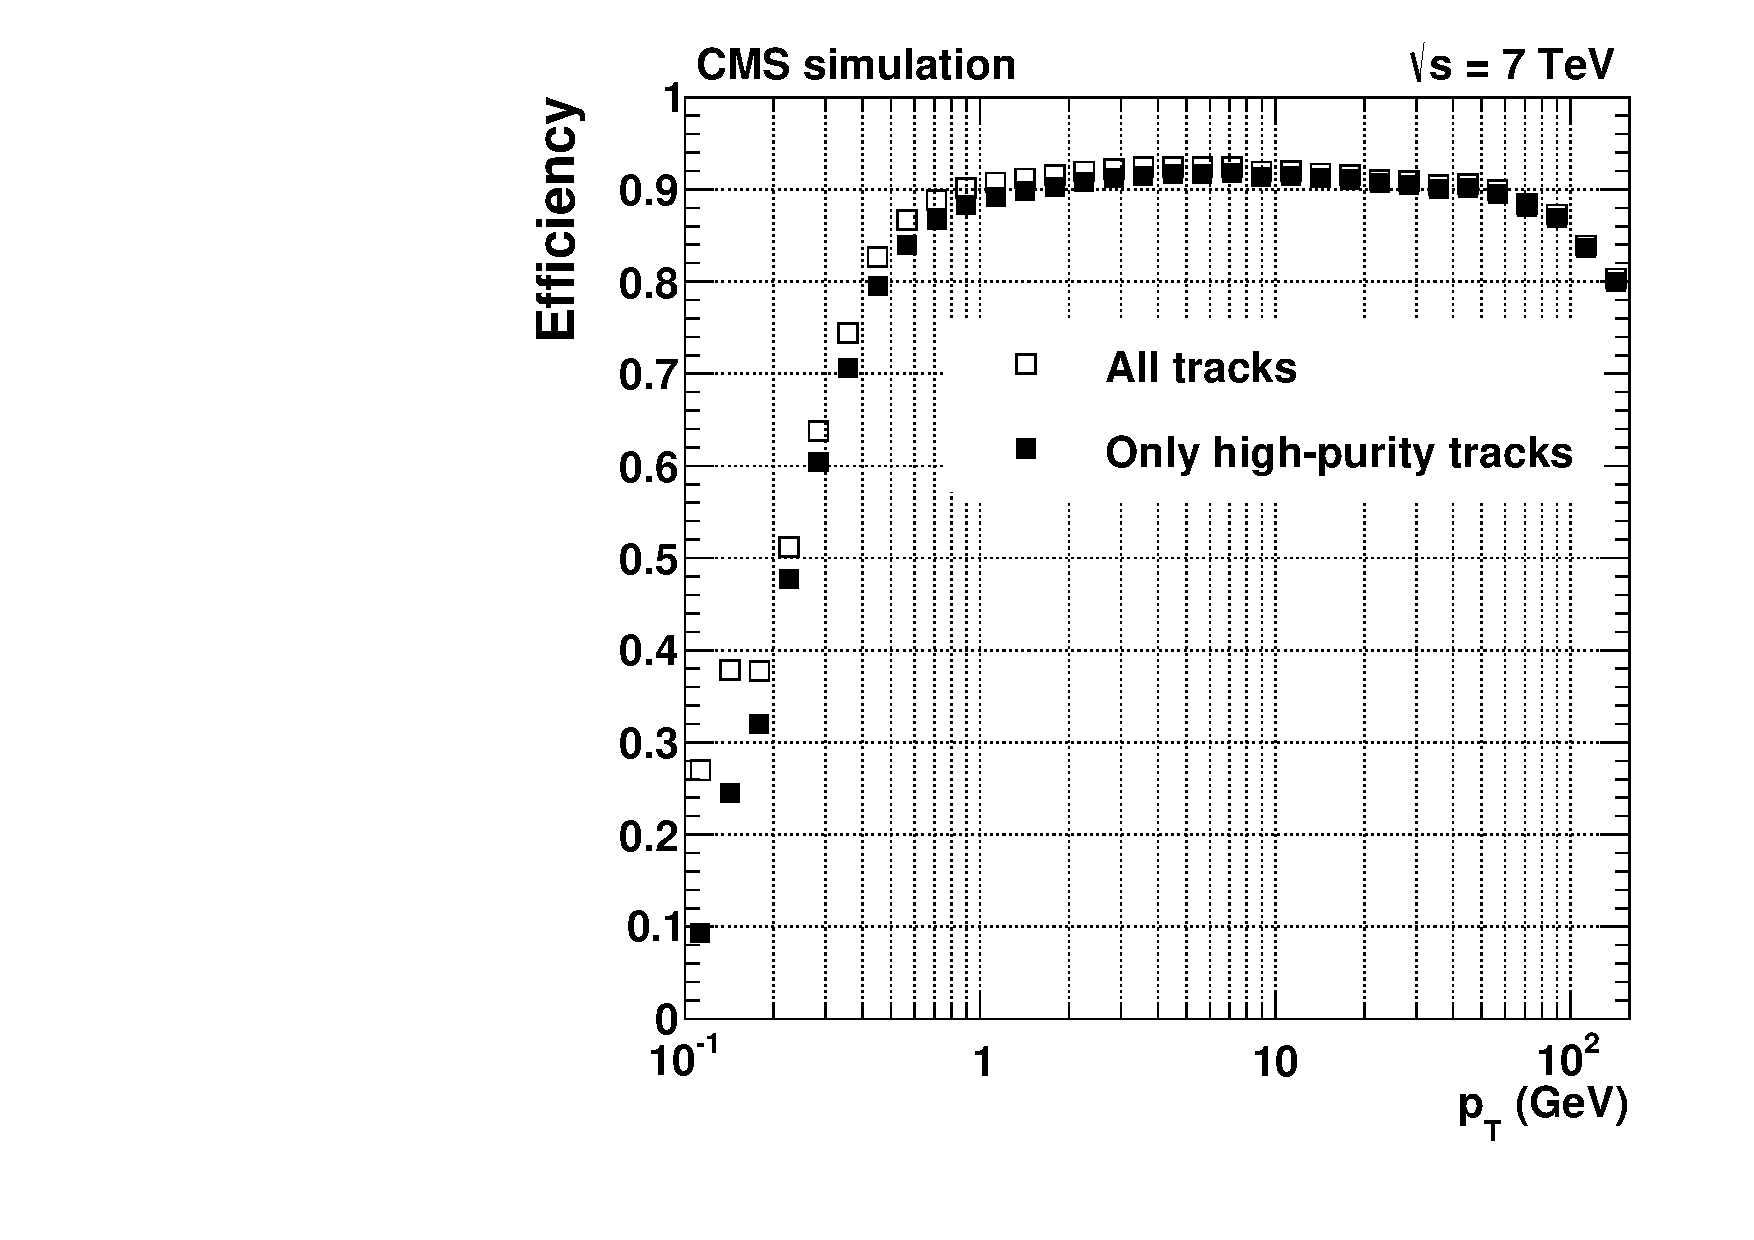
\includegraphics[width=0.65\textwidth]{figures/efficiencyVsPt.pdf}
    \caption[CMS integrated luminosity delivered and recorded over time.]{
      The integrated luminosity delivered to CMS over time by the LHC, in blue, and the portion CMS managed to record, in yellow.
      As can be seen, CMS is not 100% efficient at recording collisions. 
      It is important to note that this inefficiency is a straightforward failure to observe the events, {\it not} the purposeful rejection of events by the trigger system discussed in Section~\ref{sec:trigger}.
      Taken from \cite{lumipublic}.}
    \label{fig:intlumi}
  \end{figure}  


  The sensitivity of searches performed in CMS scales straightforwardly with the total number of collisions provided by the LHC.
  Thus far, the LHC has provided CMS with nearly 200~\fbinv across all operating periods, with the rate accelerating as the machine is pushed to the limits of its design, as shown in Figure~\ref{fig:intlumi}.
  The searches discussed in the next chapter use only the 137~\fbinv recorded by CMS during the 13~TeV runs from 2016 to 2018.
  As the total inelastic proton-proton collision cross section is approximately 69.2~mb at 13~TeV, the total number of collisions observed by CMS from 2016 to 2018 is nearly $10^{16}$.
  While this vast sample size makes very rare genuine physics processes potentially observable, it also presents a challenge in that very rare and difficult to model detector failures may pollute the dataset.
  It is prudent to adopt a conservative approach to any searches for rare new physics.

\section{The CMS Detector} \label{sec:CMS}

  While the LHC provides the collisions, it is the Compact Muon Solenoid (CMS) detector that ultimately measures the products and reconstructs each event.
  A detailed description of all of the CMS hardware and software is available in Reference~\cite{cms_tdr}, and a description of the general event reconstruction technique used at CMS, called Particle Flow, is available in Reference~\cite{particleflow}.
  This section serves as a general overview of how CMS works, sufficient to understand the searches for new physics presented later in this work.

  The particles stable enough to be detected directly by CMS come in 5 distinct varieties, namely electrons, muons, photons, charged hadrons (largely protons, pions, and charged kaons), and neutral hadrons (largely neutrons and neutral kaons).
  Figure~\ref{fig:cmsreconstruction} depicts a generic detection of each kind of particle.
  All other particles are too unstable to be measured directly, except the neutrinos.
  Neutrinos are, uniquely among Standard Model particles, both stable and invisible to CMS.
  Their presence in the products of a collision is inferred by measuring all of the visible content of an event, and noting that some energy is missing, as discussed in Section~\ref{sec:MET}.
  Any stable weakly interacting particles beyond the Standard Model produced in a collision at CMS would present a similar signature.

  \begin{figure}[h!]
    \centering
    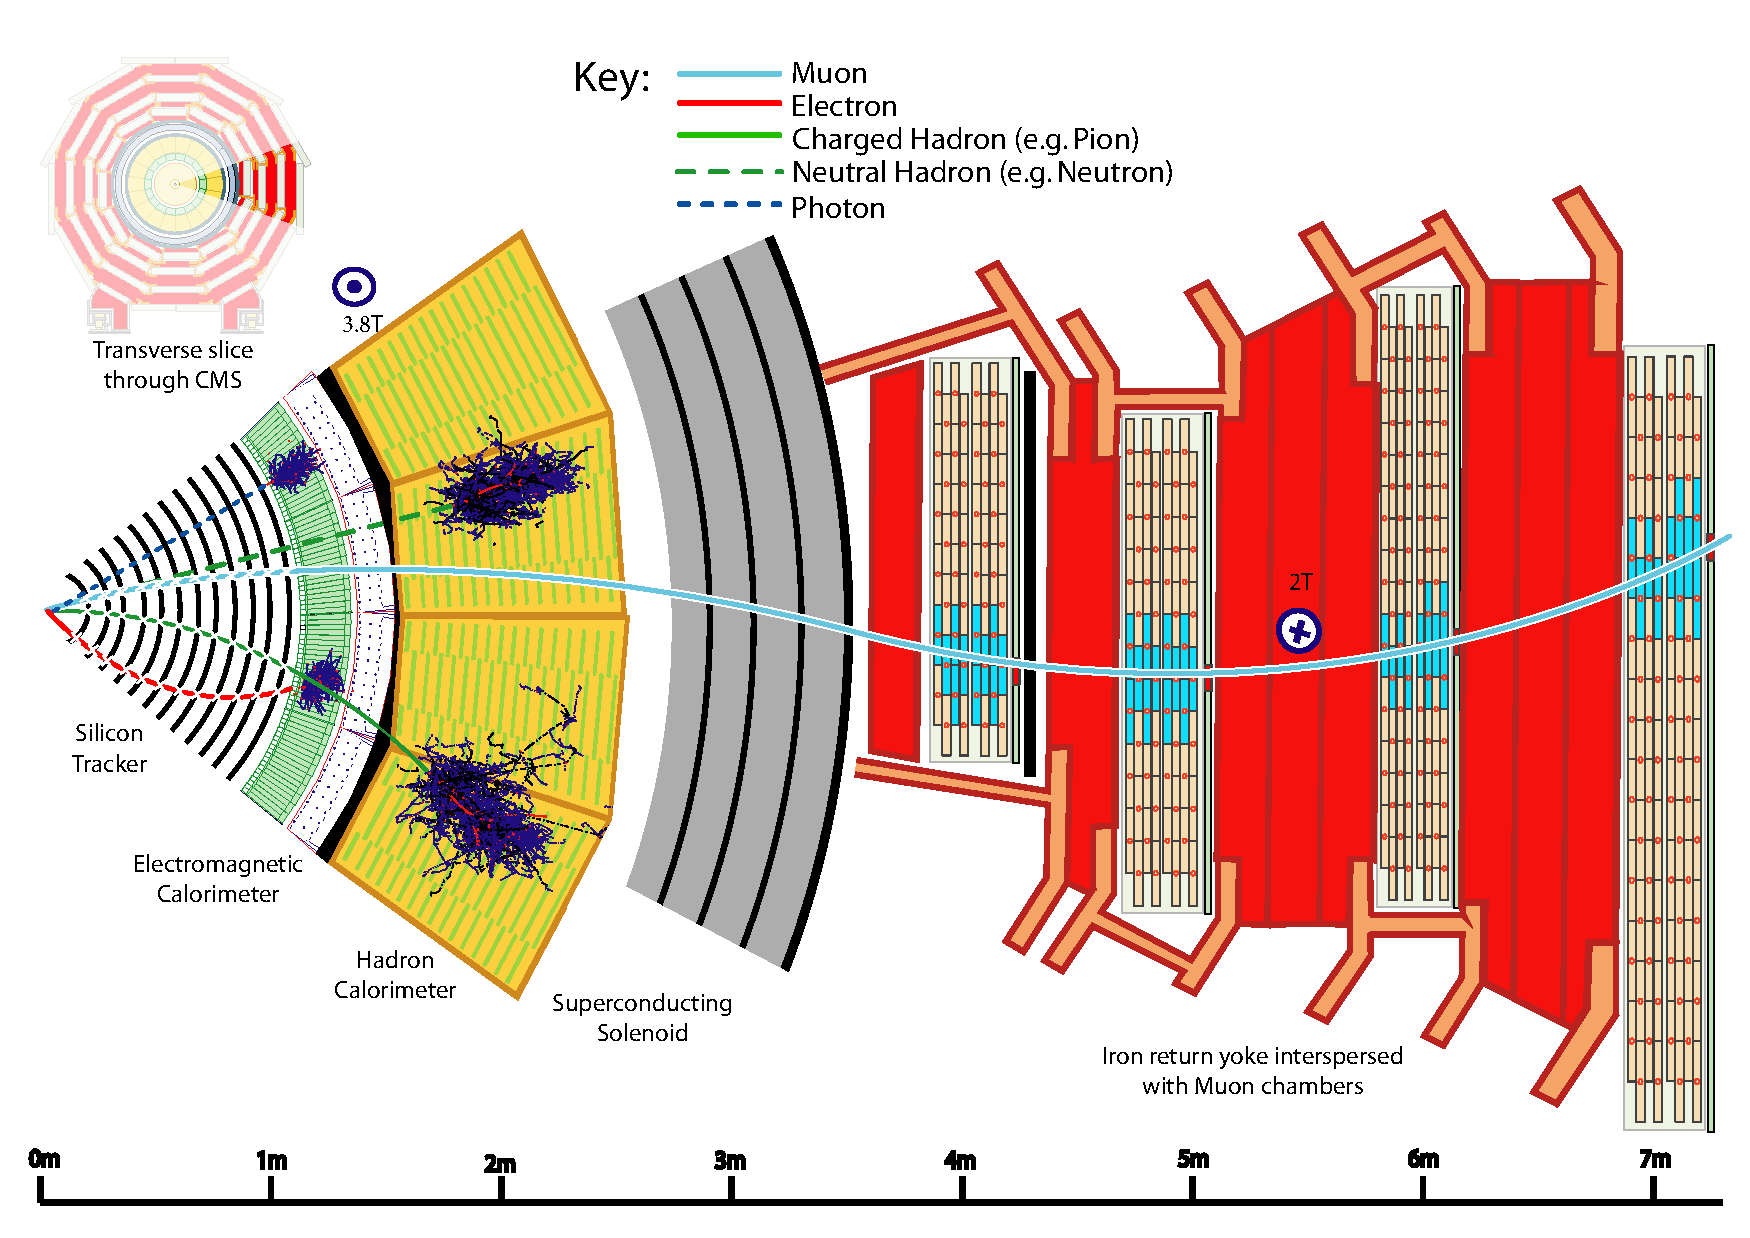
\includegraphics[width=0.85\textwidth]{figures/cmsreconstruction.pdf}
    \caption[Image depicting the experimental signatures of different types of particle at CMS.]{
      The design of CMS causes particles of different types to leave distinct experimental signatures, allowing them to be distinguished.
      The rest of this section references and explains this image.
      Taken from \cite{particleflow}.}
    \label{fig:cmsreconstruction}
  \end{figure}  

  The CMS detector is a cylinder composed of a central barrel section with two flat endcaps, each of which contain layers of different detection systems designed to provide the information necessary to distinguish the various particles that can be generated by collisions, and measure their positions and energies.
  Starting from the beam pipe, they are the tracker, the electromagnetic calorimeter, the hadronic calorimeter, and the muon system.
  The tracker and the calorimeters are inside a solenoid producing a magnetic field, while the muon system is subject only to the external, returning field of the solenoid.
  Altogether, the detector measures about 7.5 meters in radius and 21 meters in length.
  As suggested by the cylindrical detector shape, the experiment uses a cylindrical coordinate system, in which the beam axis is assigned to the z axis, and the angle in the transverse plane, $\phi$, is measured starting from a line connecting CMS to the center of the LHC ring.

  This section describes each of the subsystems, as well as the objects that are constructed using their measurements.

  \subsection{Magnet} \label{sec:magnet}

  As its name suggests, a major feature of the CMS detector is a superconducting solenoid, the largest ever built, which provides a constant 3.8~T magnetic field in the tracker and calorimeters.
  This magnetic field curves the trajectories of charged particles, allowing for a determination of their charges and assisting in the measurement of their masses and energies, contributing to highly accurate identification of particles.
  
  CMS is compact in part to make it possible to fit the bulk of the detector inside this single solenoid.
  This maximizes the strength and consistency of the magnetic field, which in turn maximizes the precision with which particle positions, and the curvatures of their trajectories, can be measured.

  In Figure~\ref{fig:cmsreconstruction}, one can see the path of an electron (orange) curving sharply, in a direction indicating that it is negatively charged.
  Similarly, the path of a charged hadron (solid green) curves in the opposite direction, indicating a positive charge.
  A positively charged muon (blue) curves first one way, then the reverse once the field flips after exiting the solenoid.
  Neutral particles (dotted lines) do not curve at all.

  \subsection{Tracker} \label{sec:tracker}

  The silicon tracker is the innermost detector system and is primarily responsible for measuring the positions of charged particles.  
  In Figure~\ref{fig:cmsreconstruction}, the trajectories of neutral particles are represented with dotted lines, to indicate that they do not actually leave those tracks in the detector.
  The tracker is critically important for the disappearing tracks search covered in Section~\ref{sec:distracks}, and so is described here in more detail than the other detector systems.

  \begin{figure}[h!]
    \centering
    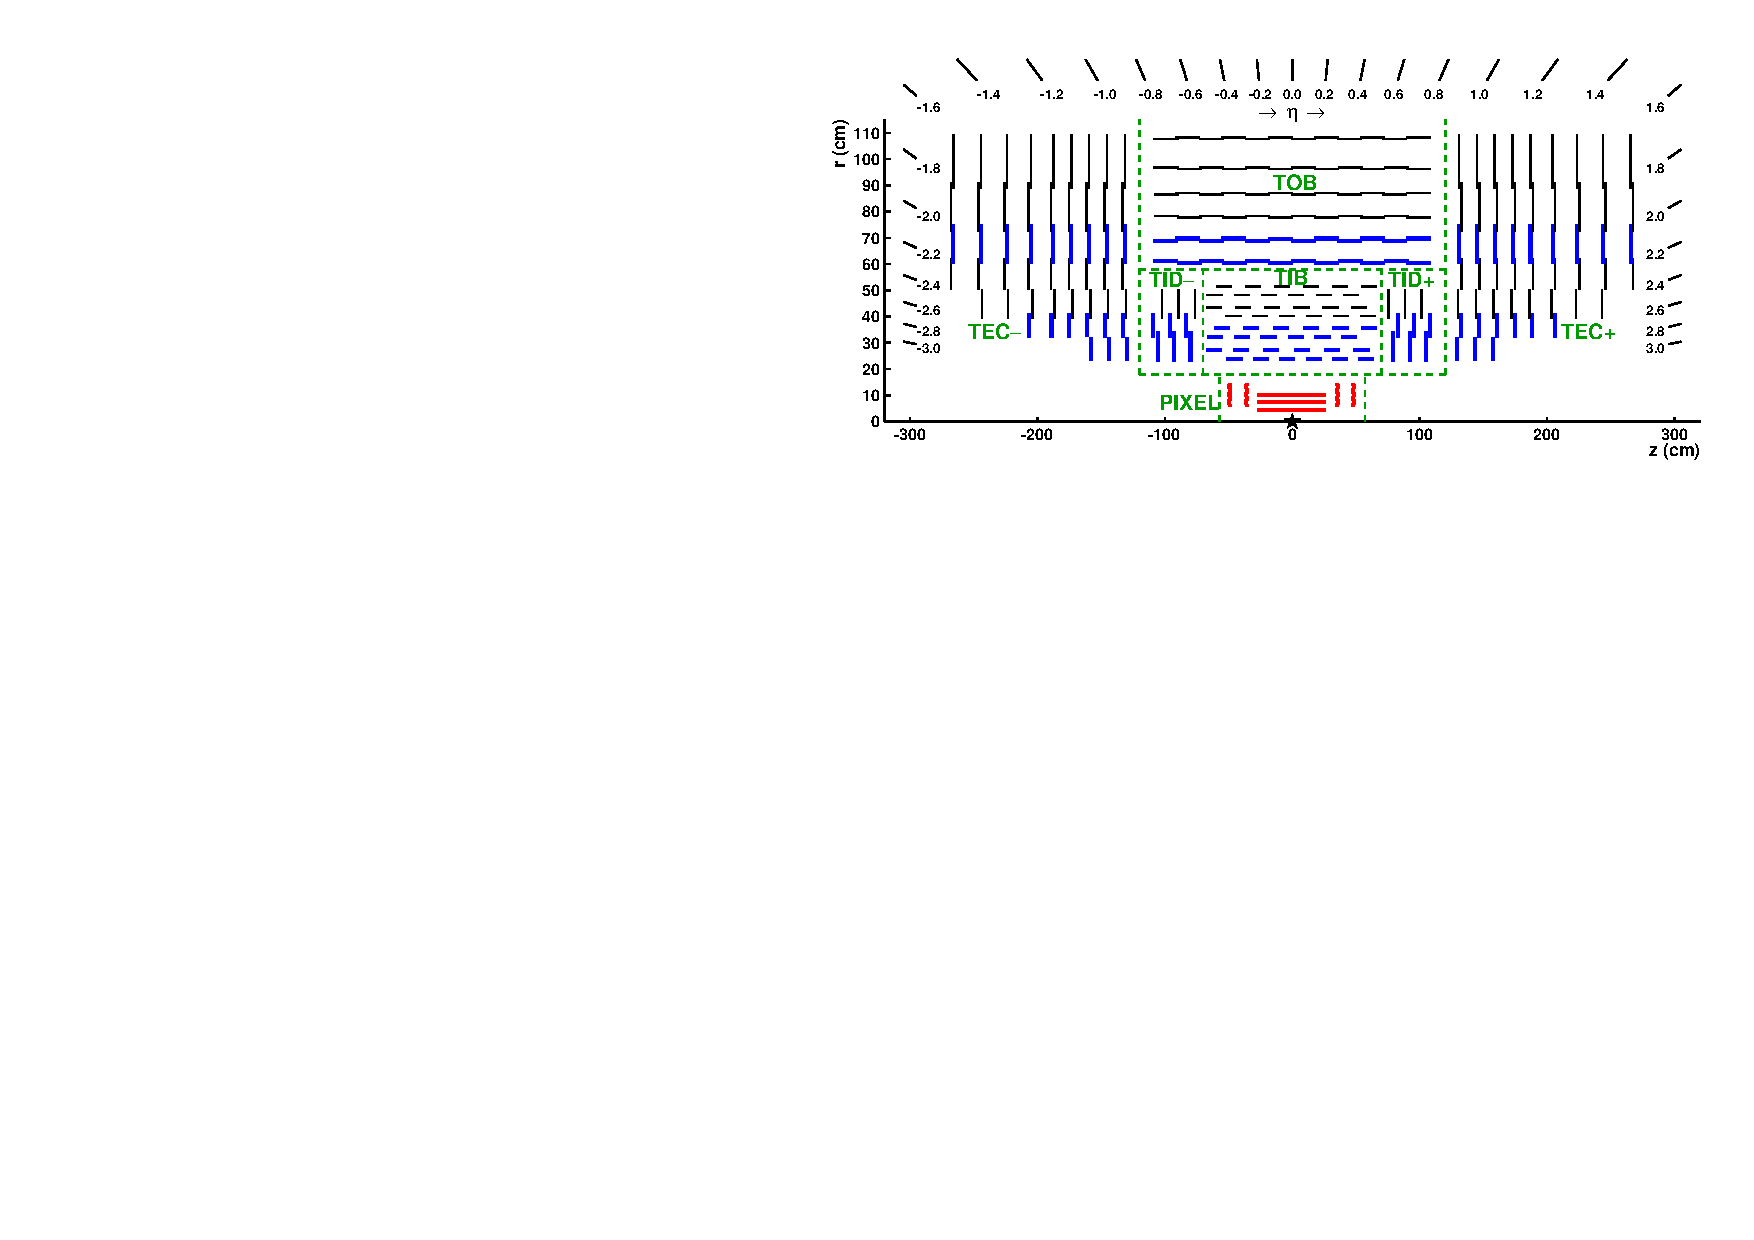
\includegraphics[width=0.75\textwidth]{figures/TrackerLayout.pdf}
    \caption[Layout of the tracker up to 2016.]{
      A slice of the CMS tracker in the $r-z$ plane, with the inner pixel tracker (red) in the 3-layer configuration used until 2016.
      In 2017 and 2018, the pixel tracker was upgraded with a 4th layer.
      The tracker is symmetric about the beam axis ($r=0$); one should imagine rotating this image around the horizontal axis to form a cylinder, to visualize the tracker's 3-dimensional form.
      The labels in green text denote tracker subsystems, the Tracker End Cap, the Tracker Inner Disk, the Pixel Tracker, the Tracker Inner Barrel, and Tracker Outer Barrel.
      The interior subsystems have more miniaturized detector elements and, therefore, better resolution.
      Taken from \cite{cmstracking}.}
    \label{fig:trackerlayout}
  \end{figure}  

  \begin{figure}[h!]
    \centering
    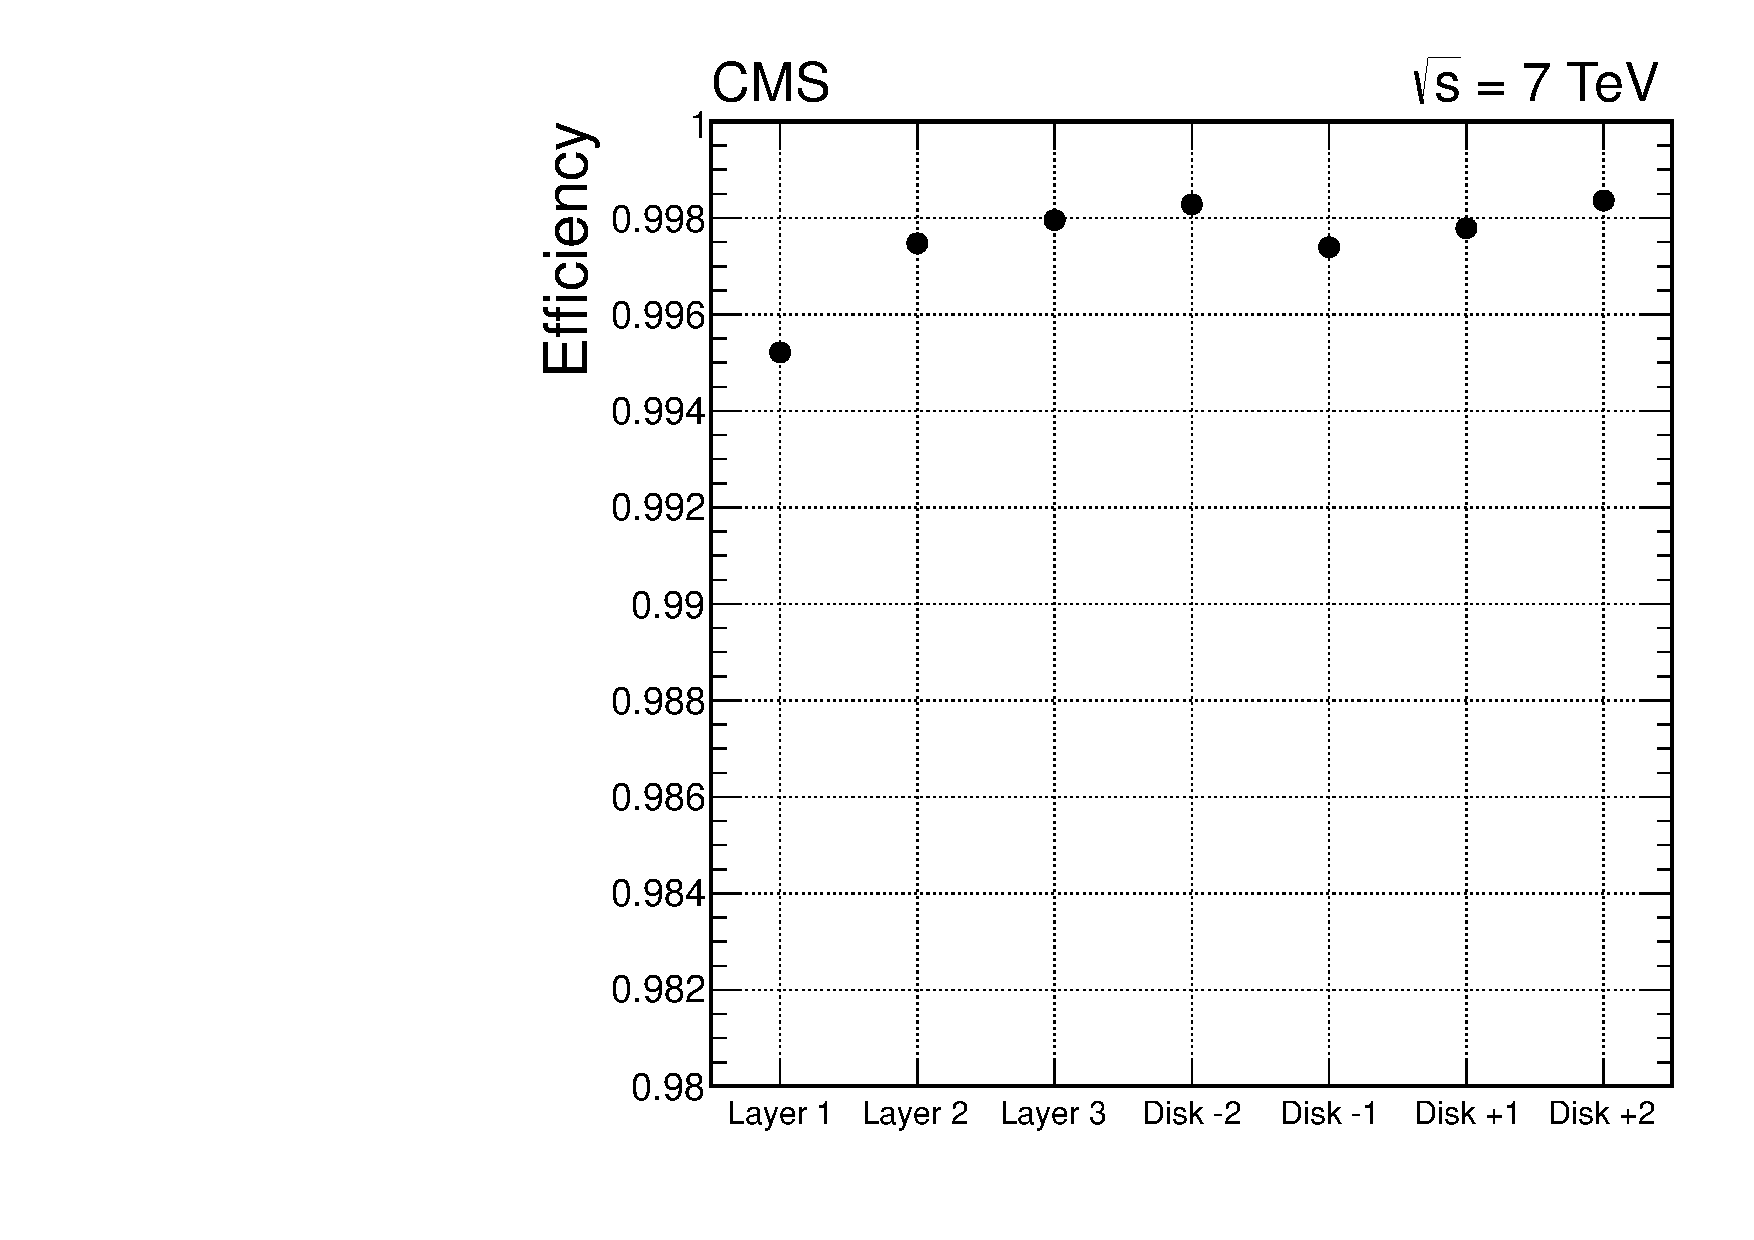
\includegraphics[width=0.65\textwidth]{figures/hitefficiency.pdf}
    \caption[Efficiency for a genuine particle to leave an expected hit in the CMS tracker.]{
      The efficiency for a genuine charged particle to produce an expected hit in the various components of the CMS pixel tracker, in the configuration used in 2016 and earlier. 
      Fake tracks may have many missing expected hits, but more than one or perhaps two is extremely rare in tracks produced by genuine particles.
      The probability for a neutral particle to produce a hit is small, and the probability to leave enough to produce a track is negligible.
      Taken from \cite{cmstracking}.}
    \label{fig:hitefficiency}
  \end{figure}  

  As shown in Figure~\ref{fig:trackerlayout}, the tracker is composed of several discrete layers.
  When a charged particle passes through a layer, it usually causes a measurable current to flow in the silicon, and is said to have produced a ``hit.''  
  As shown in Figure~\ref{fig:hitefficiency}, the probability for a genuine particle to leave a hit is near but not quite unity, so a missing hit where one would be expected is credible but cause for skepticism.
  Each event produces an intimidating array of these discrete hits throughout the tracker, which must then be connected by the track reconstruction algorithm into particle tracks.
  CMS uses an iterative procedure described in Reference~\cite{cmstracking}, in which clean, high energy, isolated tracks are reconstructed first so that their hits may be removed from the pool, followed by the next most obvious tracks, and so on, dramatically simplifying the computational complexity of each step.
  The early iterations that produce the tracks judged to be of highest quality find only those tracks with transverse momenta at least 0.3~GeV, and no iteration can produce a track with transverse momentum below 0.1~GeV, so that particles of such low energy are effectively invisible to CMS.
  Note that, due to the strong magnetic field present in the tracker, particles with energies lower than around 0.1 GeV travel in such tight spirals that reconstruction becomes infeasible.
  Although this is normally insignificant, since these particles are not typically important to an event's overall characterization, this fact allows for the existence of disappearing tracks, in which a high energy charged particle decays to a trackless neutral particle and a charged particle of such low energy that it is not reconstructed.
  Additionally, all tracks must be composed of at least 3 hits.

  The performance is outstanding, especially for tracks passing the sophisticated ``high purity'' selection applied by the vast majority of CMS analyses. 
  Figure~\ref{fig:trackfakerate} shows the fake rate of this procedure, less than 5\% for tracks in the intermediate energy range, and further suppressible with additional cleaning selections like those of the disappearing tracks search covered in Section~\ref{sec:distracks}.
  Figure~\ref{fig:trackefficiency} shows the efficiency to reconstruct tracks successfully for the three most common varieties of charged particles measured by CMS, namely muons (left), electrons (center), and pions (right), approaching unity in all cases for higher energy tracks in the barrel region of the tracker.

  \begin{figure}[h!]
    \centering
    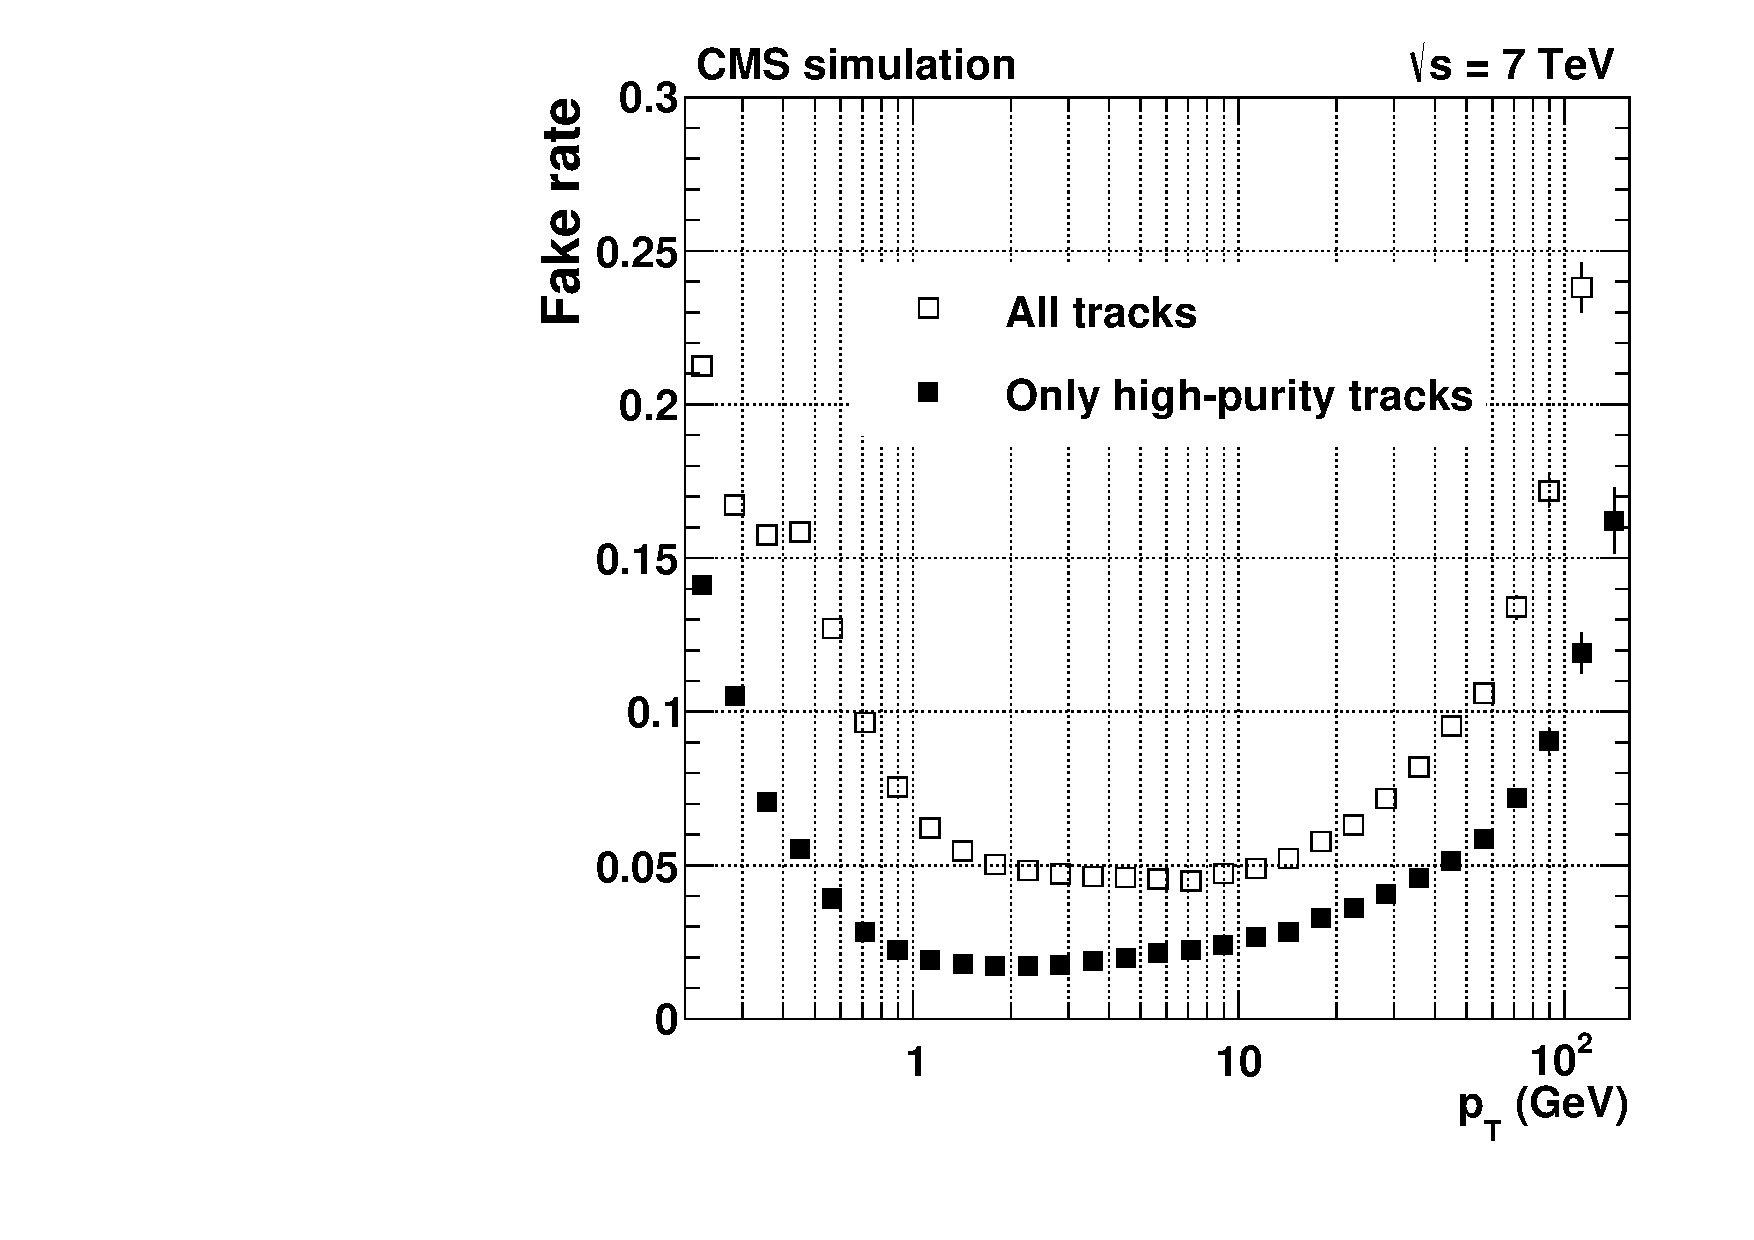
\includegraphics[width=0.65\textwidth]{figures/fakerateVsPt.pdf}
    \caption[Track fake rate.]{
      The CMS track fake rate as a function of \pt, in the configuration used in 2016 and earlier. 
      The sophisticated high purity selection aims to suppress the fake rate without badly affecting efficiency and is applied in the vast majority of CMS analyses. 
      Taken from \cite{cmstracking}.}
    \label{fig:trackfakerate}
  \end{figure}  

  \begin{figure}[h!]
    \centering
    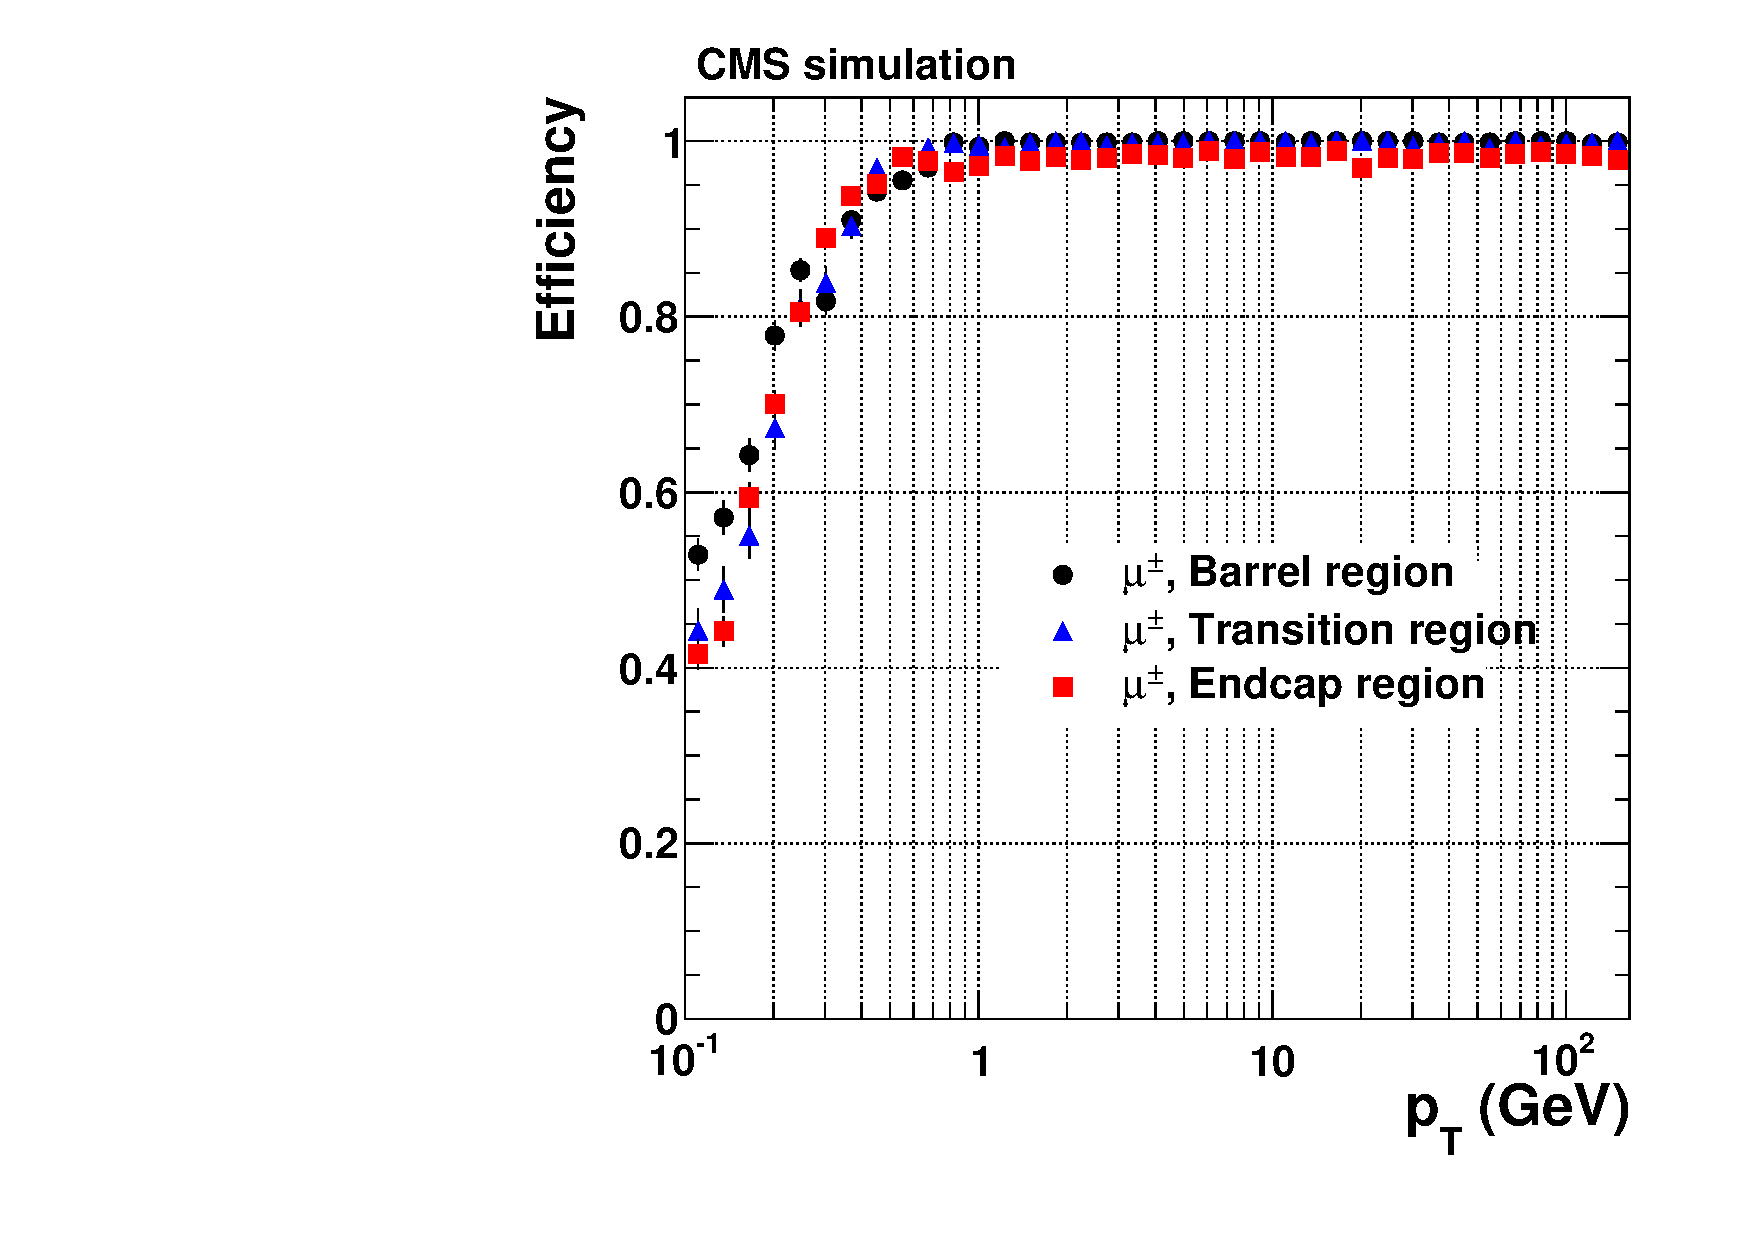
\includegraphics[width=0.3\textwidth]{figures/mu/efficiencyVsPt.pdf}
    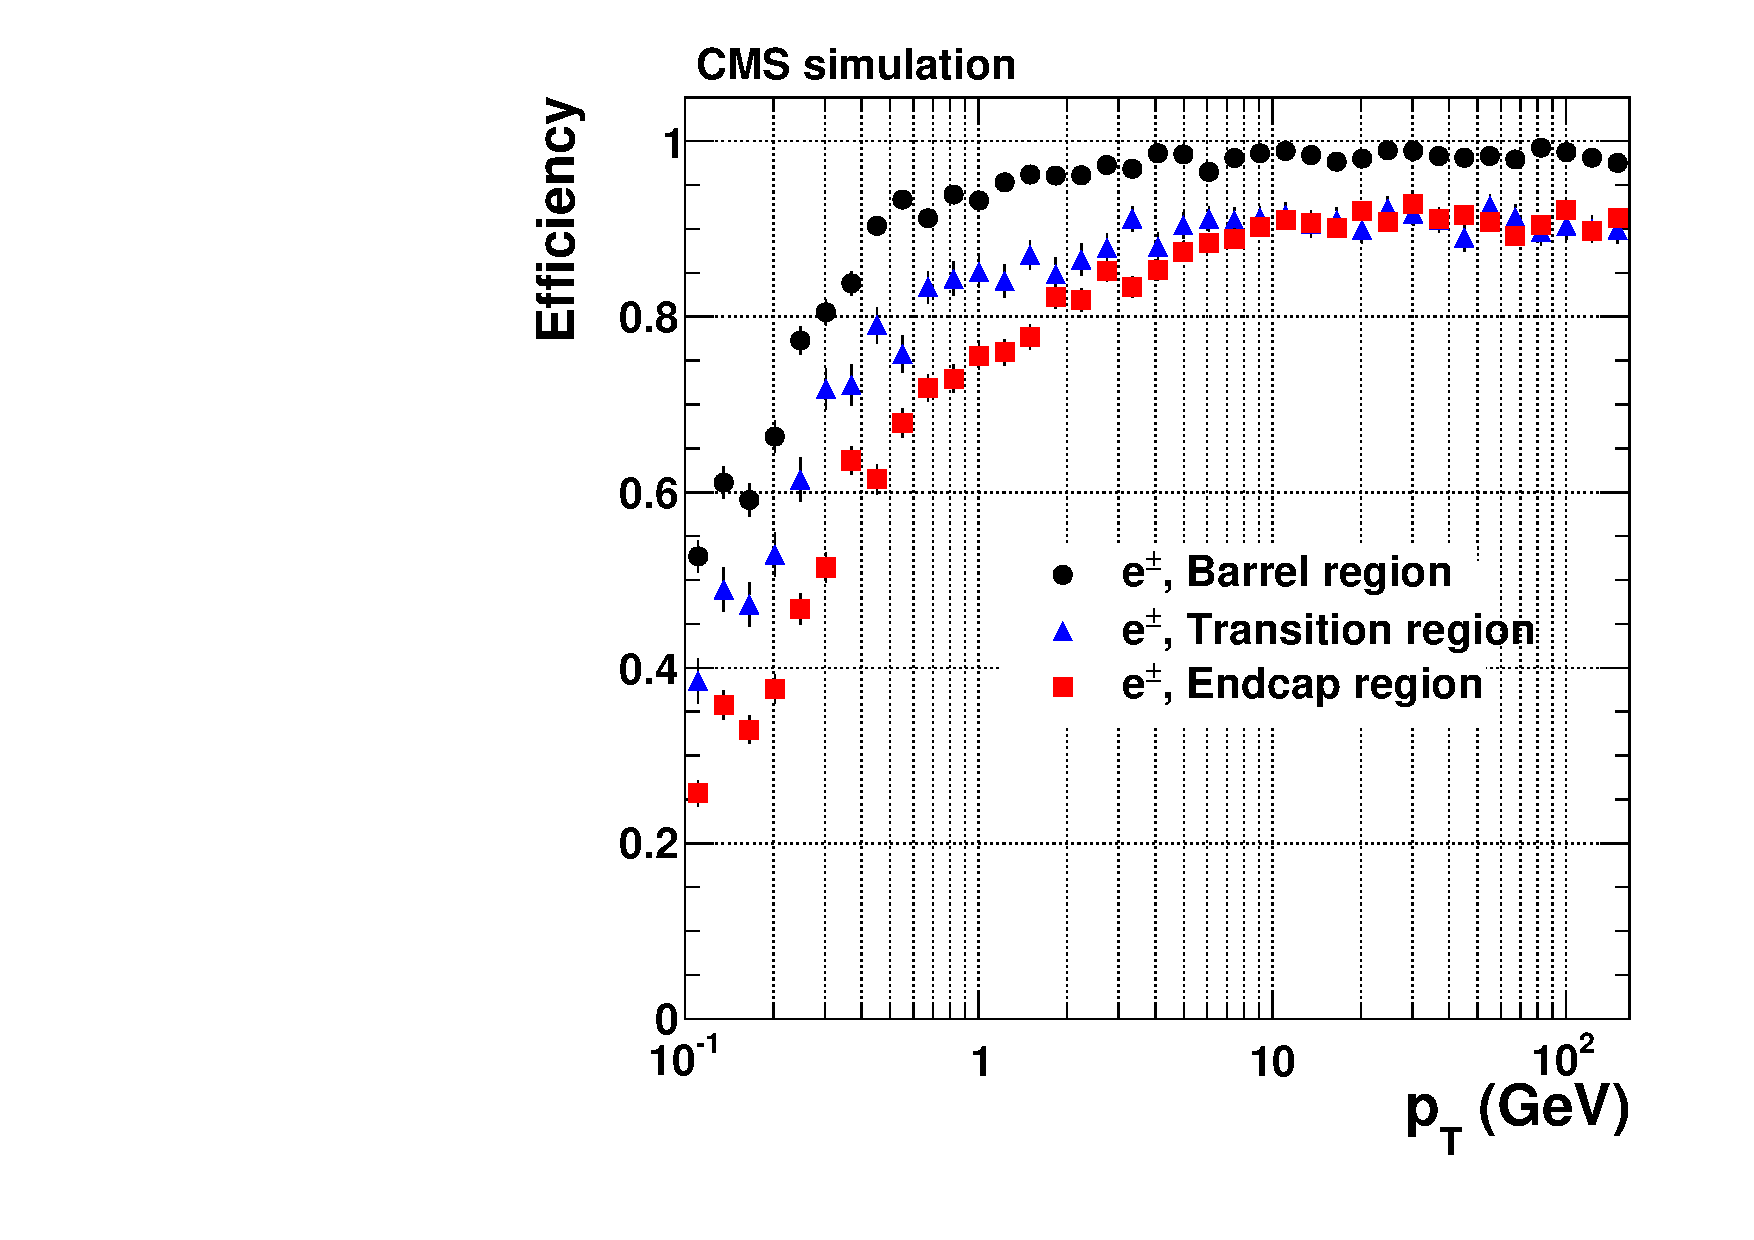
\includegraphics[width=0.3\textwidth]{figures/el/efficiencyVsPt.pdf}
    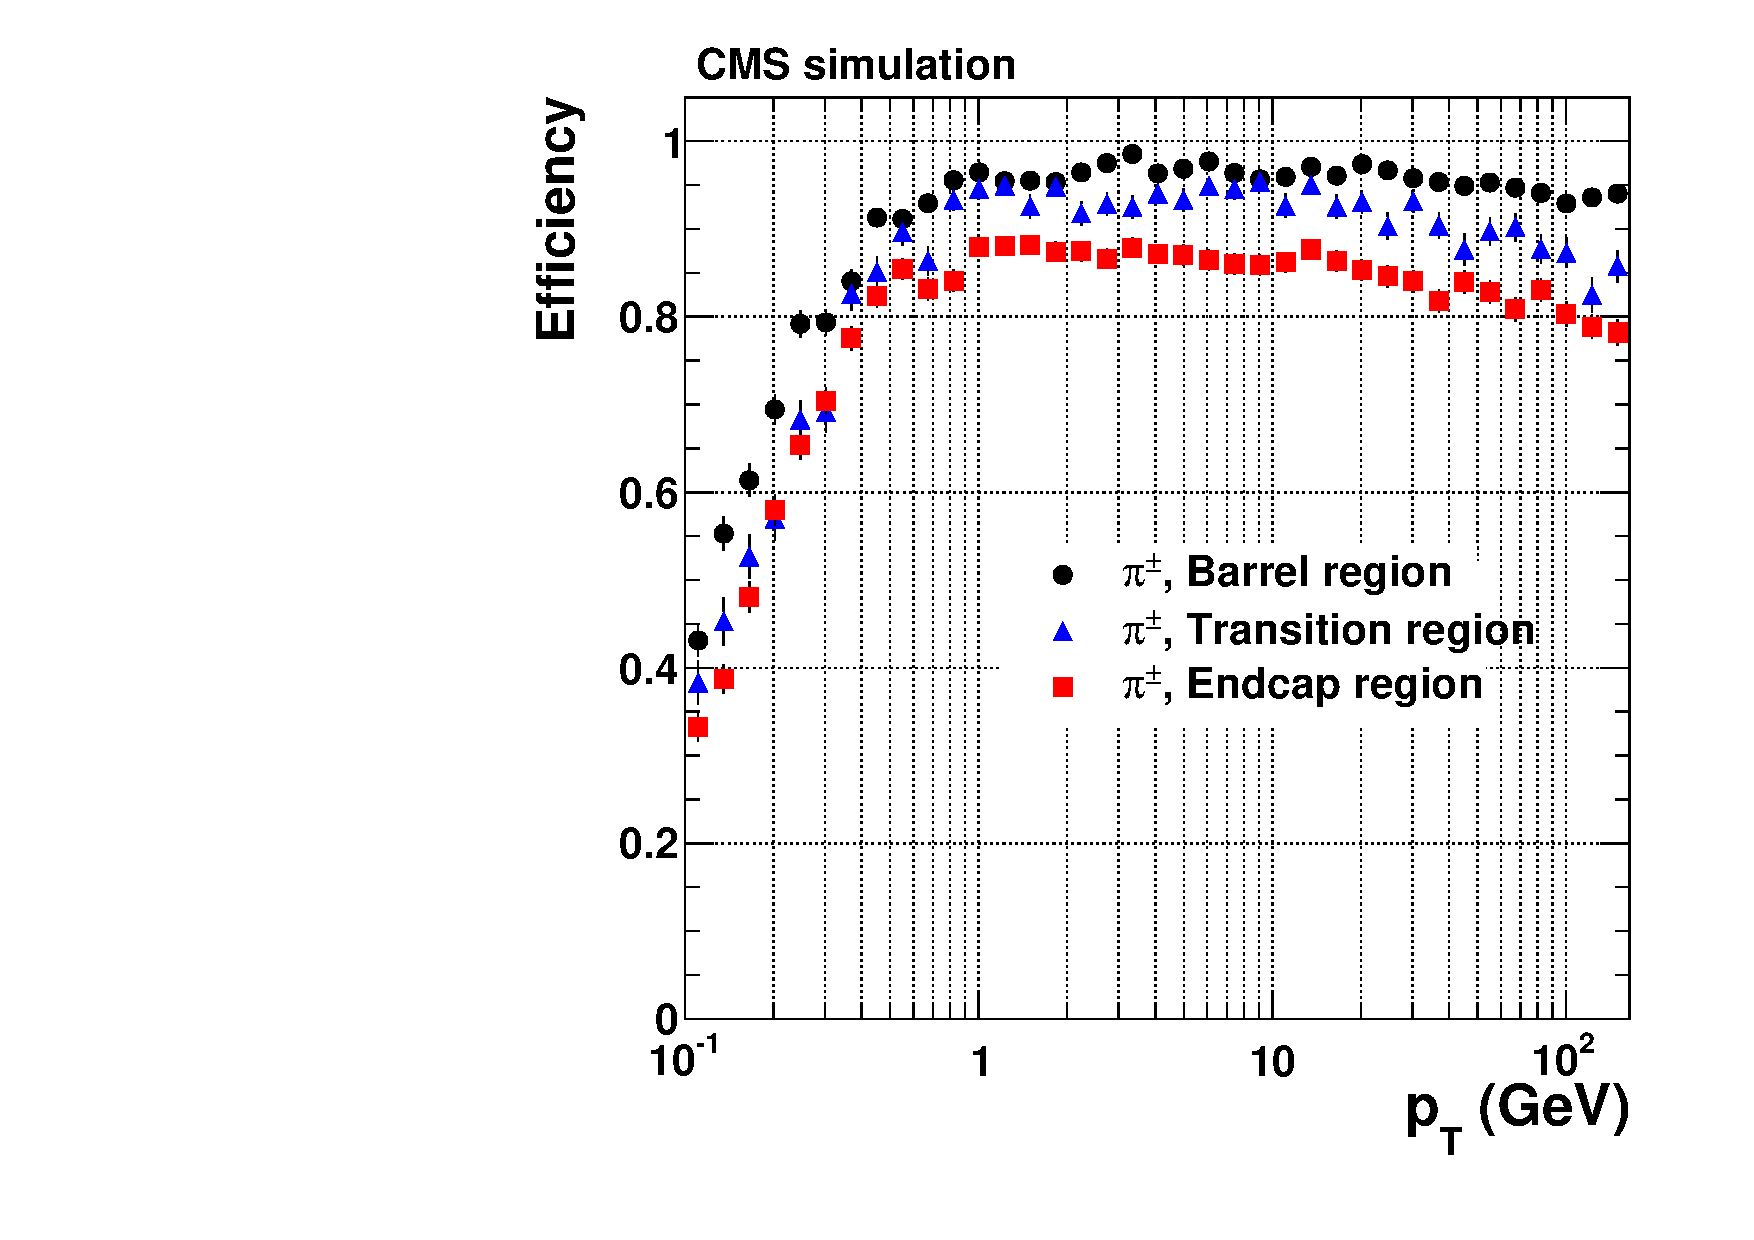
\includegraphics[width=0.3\textwidth]{figures/pi/efficiencyVsPt.pdf}
    \caption[Track reconstruction efficiency.]{
      The CMS track reconstruction efficiency for (left) muons, (center) electrons, and (right) pions, split by detector region as a function of \pt, in the configuration used in 2016 and earlier. 
      Muons are by far the cleanest objects at CMS as they are massive enough to avoid strong perturbations by tracker material, and lack nuclear interactions.
      Electrons are lighter and so are vulnerable to tracker interactions, experiencing strong bremsstrahlung losses, while pions can undergo nuclear interactions.
      Taken from \cite{cmstracking}.}
    \label{fig:trackefficiency}
  \end{figure}  

  \begin{figure}[h!]
    \centering
    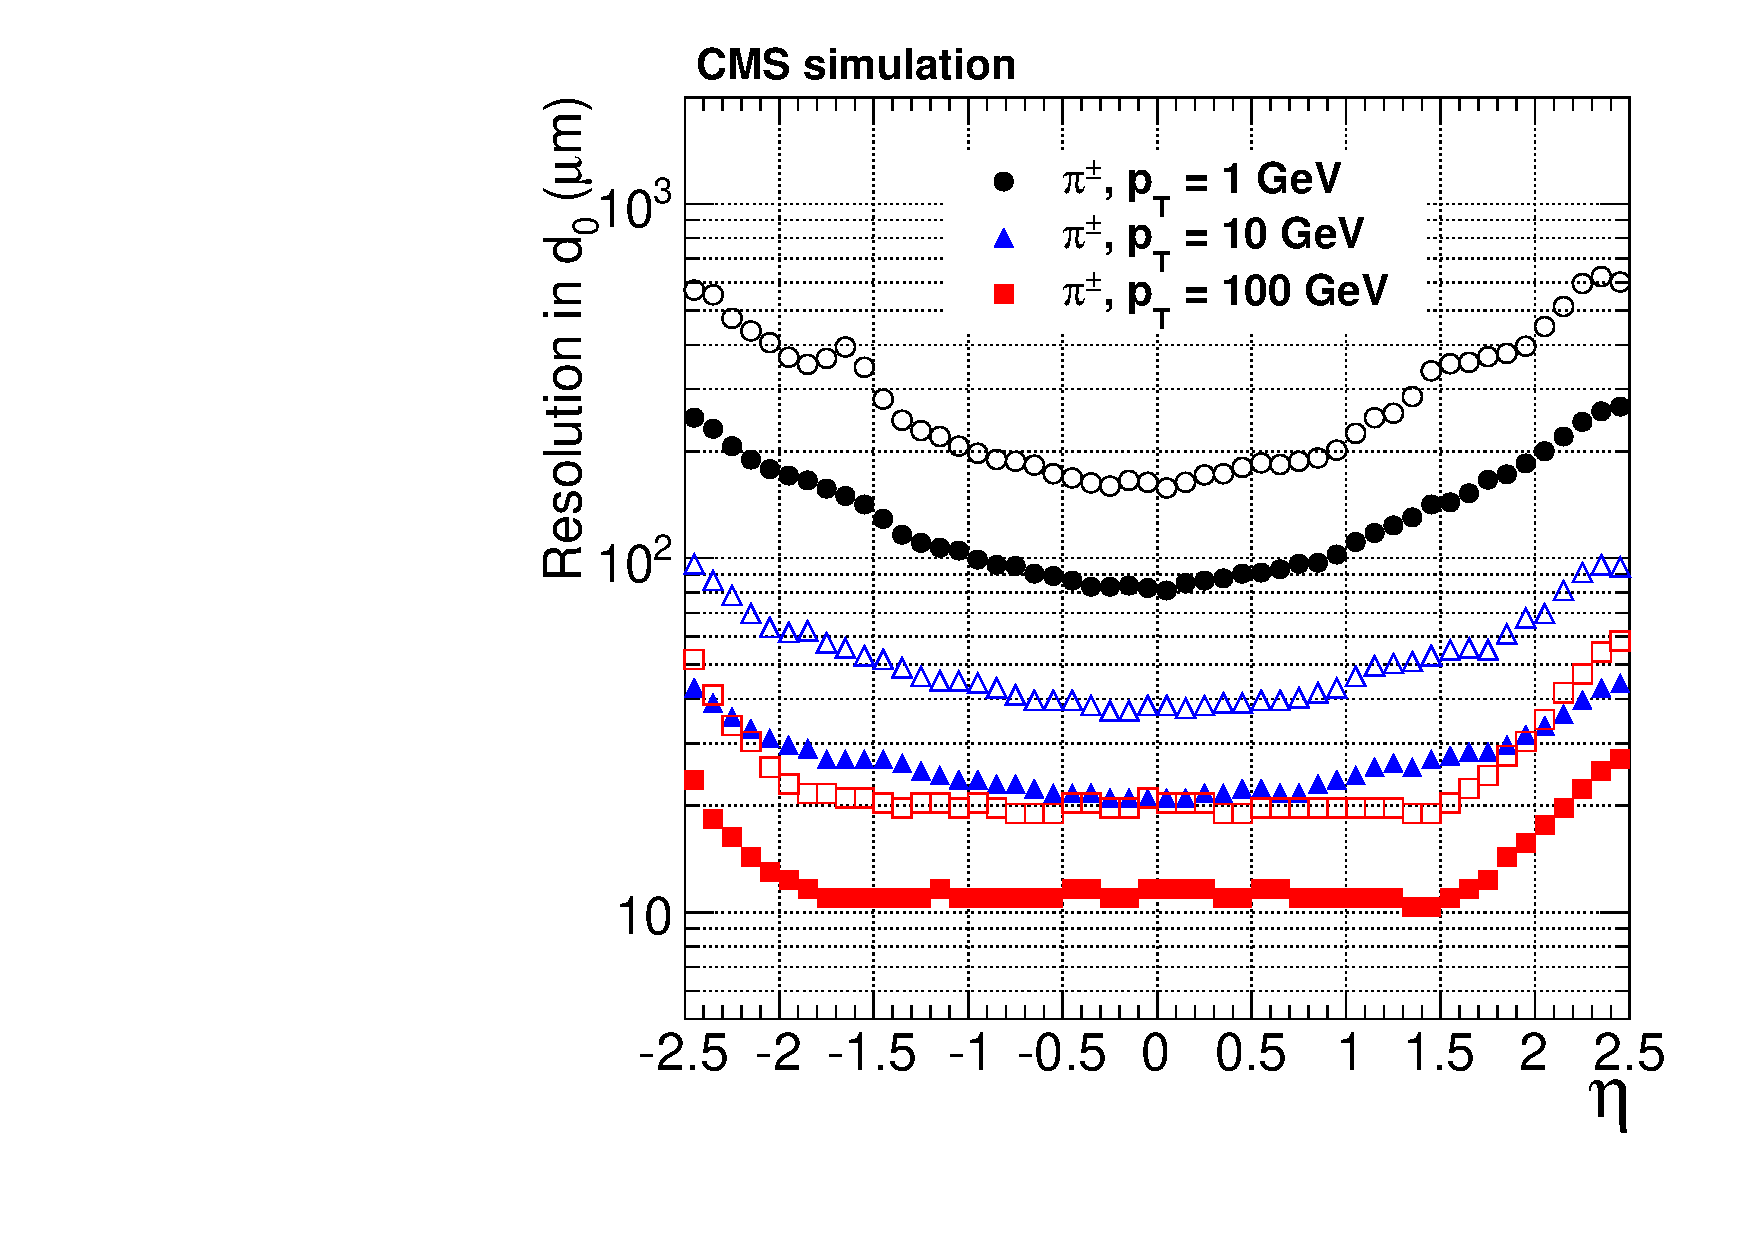
\includegraphics[width=0.4\textwidth]{figures/pi/resolutionD0VsEta.pdf}
    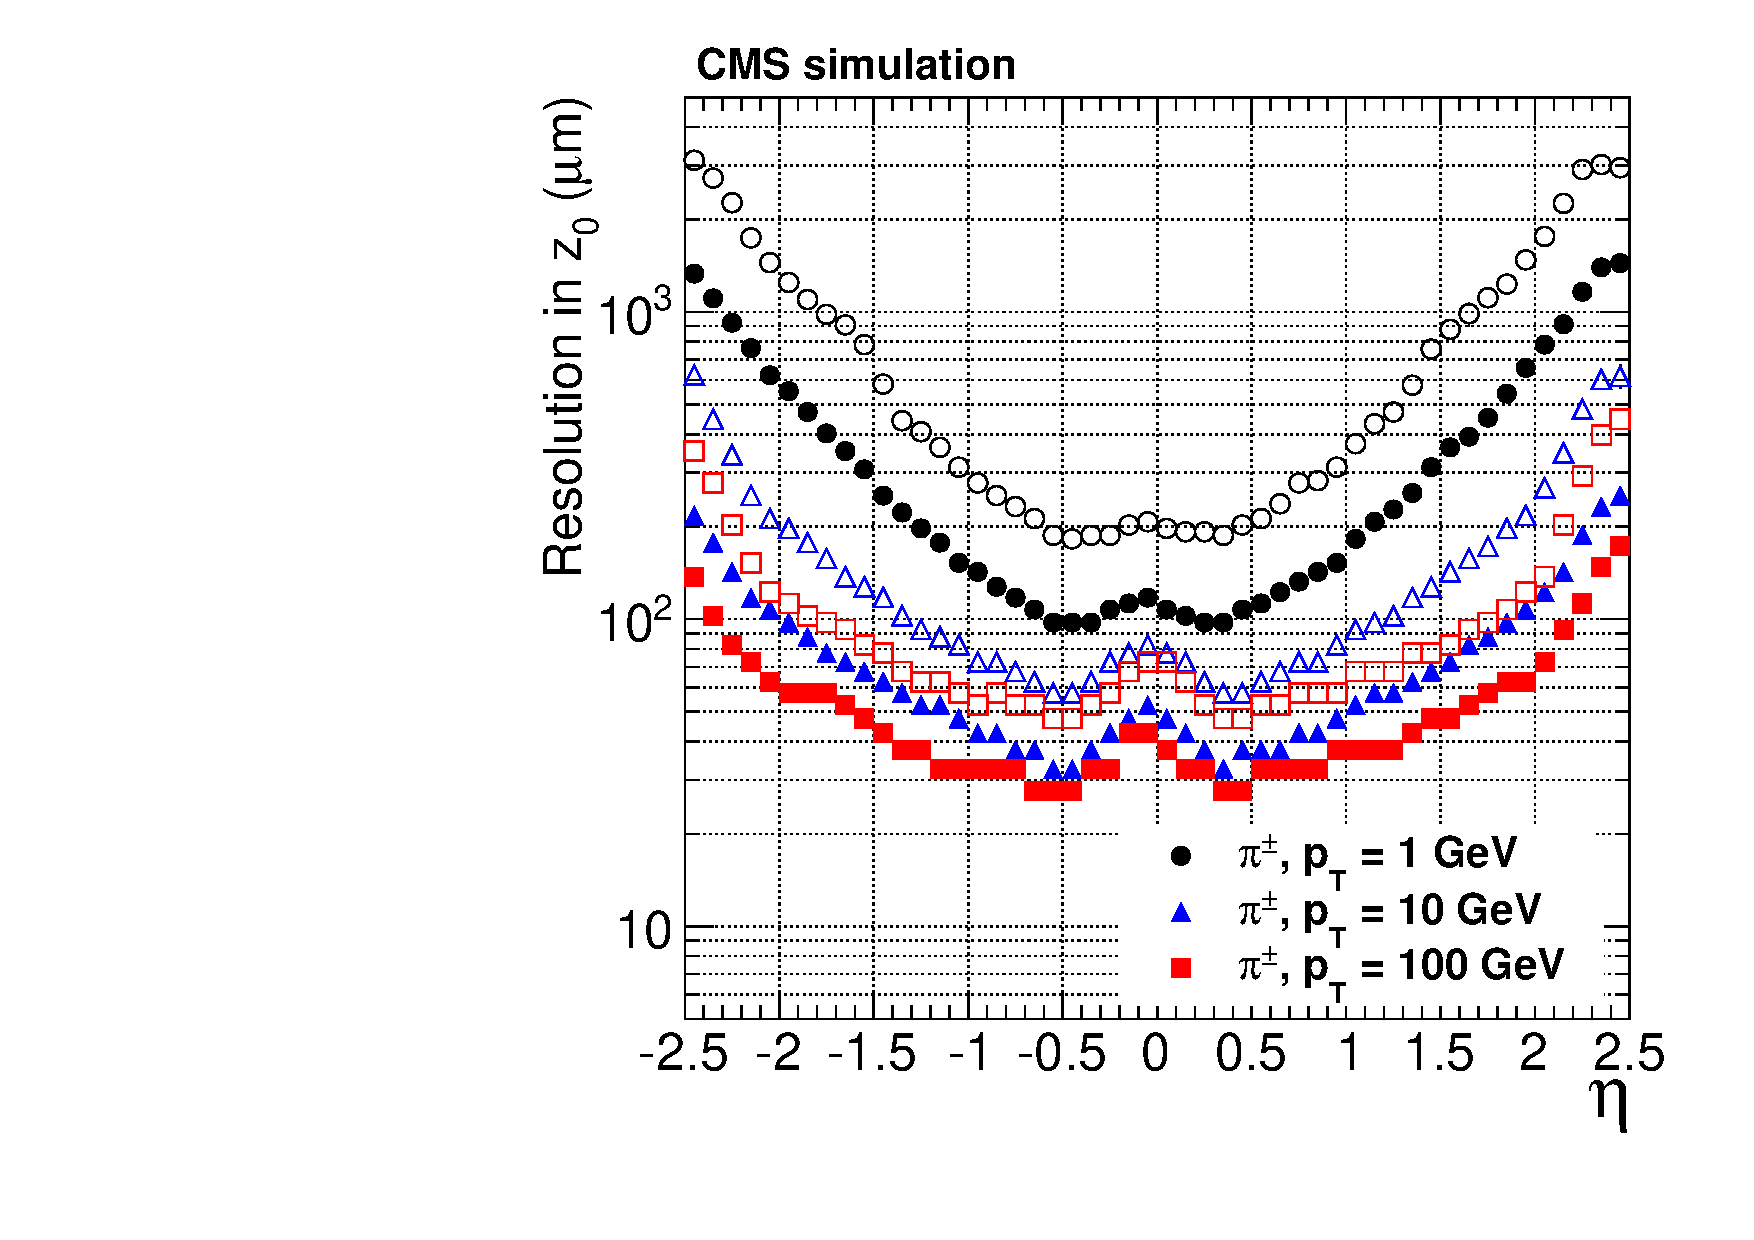
\includegraphics[width=0.4\textwidth]{figures/pi/resolutionDzVsEta.pdf}
    \caption[Impact parameter resolution in the CMS tracker.]{
      The CMS tracker has micron-level impact parameter resolution, for both (left) the transverse plane and (right) the z direction.
      Solid markers indicate the half-width of the 68\% confidence interval, while open markers indicate 90\% confidence.
      With this resolution, a track reconstructed with an impact parameter of more than a few hundred microns is likely a fake, from a pileup vertex, or from a secondary vertex produced by a decaying particle like a bottom hadron.
      Taken from \cite{cmstracking}.}
    \label{fig:trackresolution}
  \end{figure}  

  The tracker detection elements are smaller and consequently provide better localization in interior layers of the tracker, with the pixel detector components only approximately 100 $\mu$m across.
  As a general guideline, no element in the tracker is permitted to have an expected probability of a hit greater than 1\% per bunch crossing, to maintain a low probability of tracks intersecting.
  This structure produces outstanding sub-millimeter resolution of a track's origin, shown in Figure~\ref{fig:trackresolution}, allowing tracks originating from collisions only microns apart to be separated, and tracks originating from decays of particles with decay lengths on the order of a millimeter to be identified.
  The former is important for rejection of pileup, and the latter for identification of jets originating from bottom quark hadrons.

  \begin{figure}[h!]
    \centering
    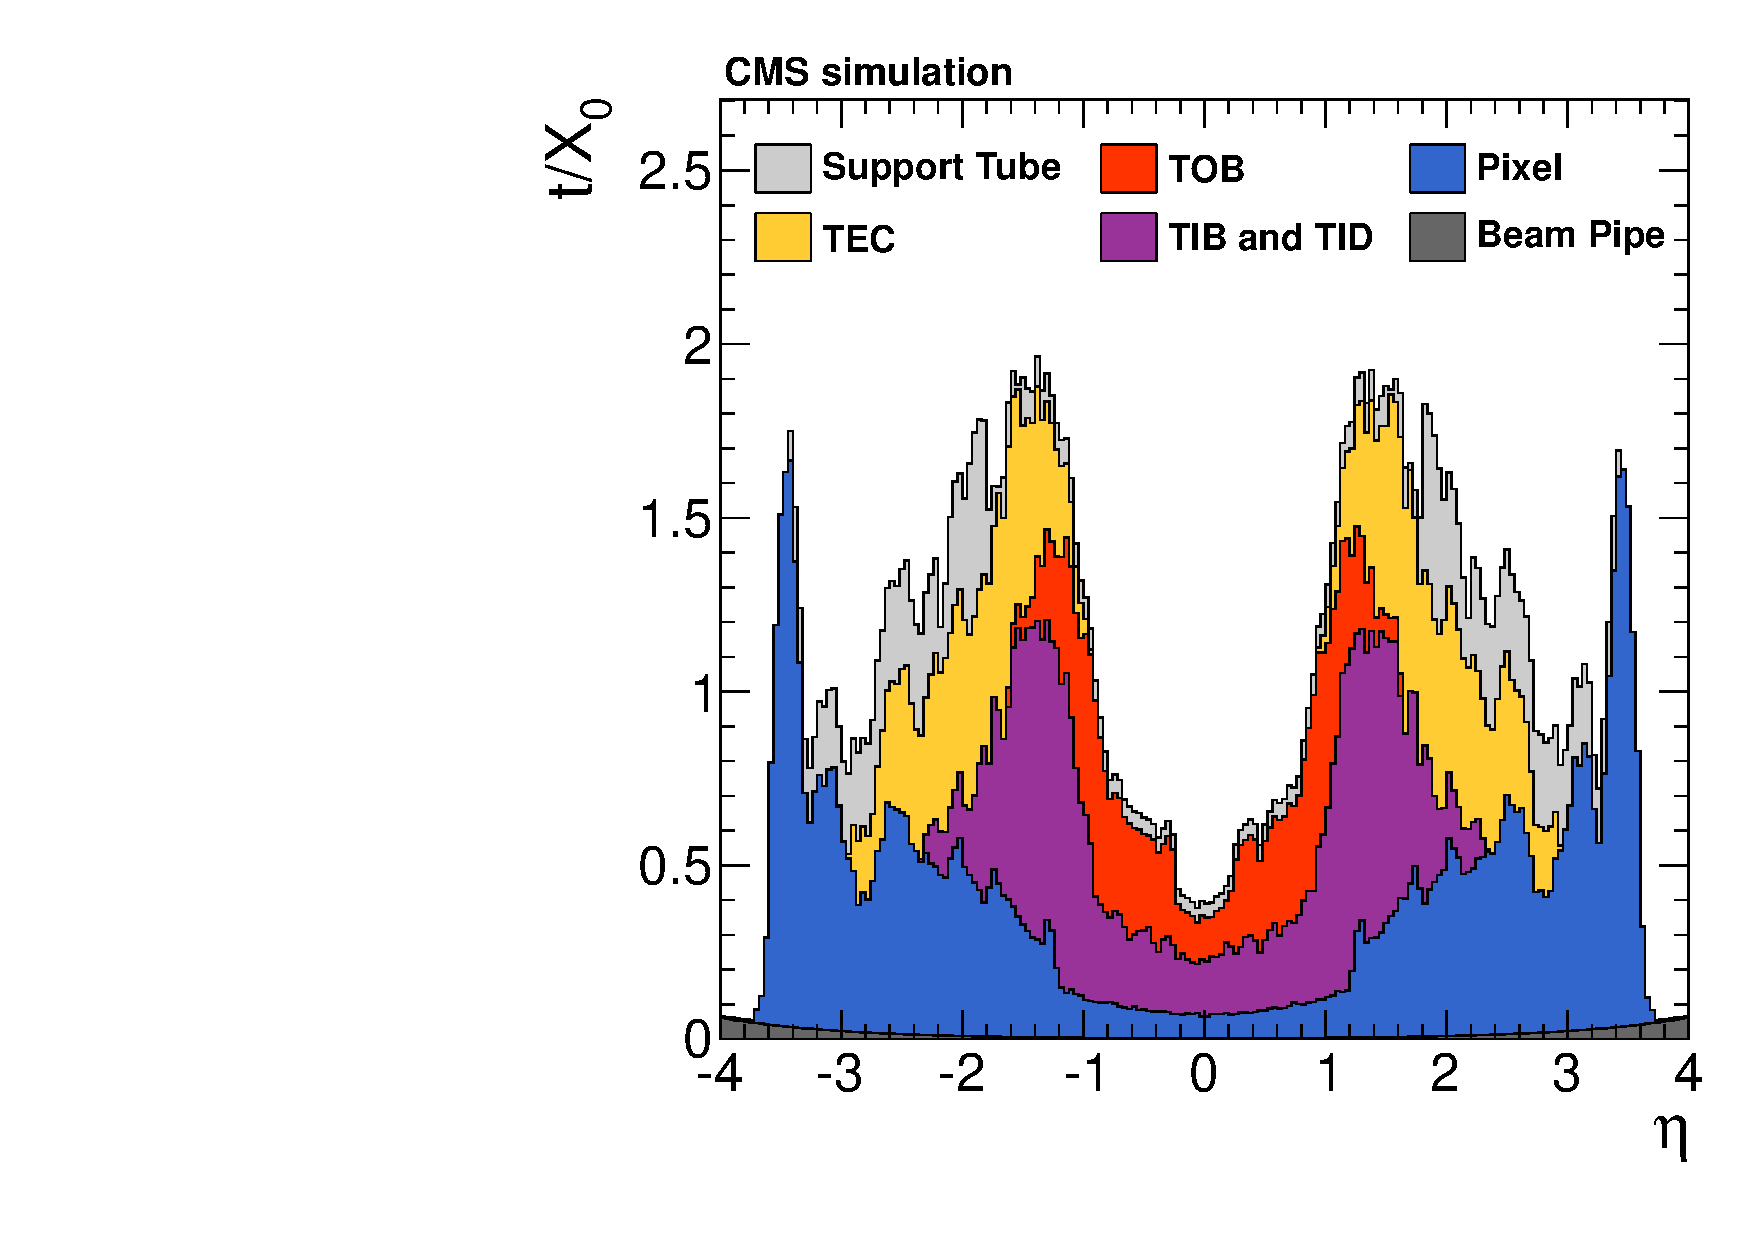
\includegraphics[width=0.4\textwidth]{figures/MaterialBudget_RadLengths.pdf}
    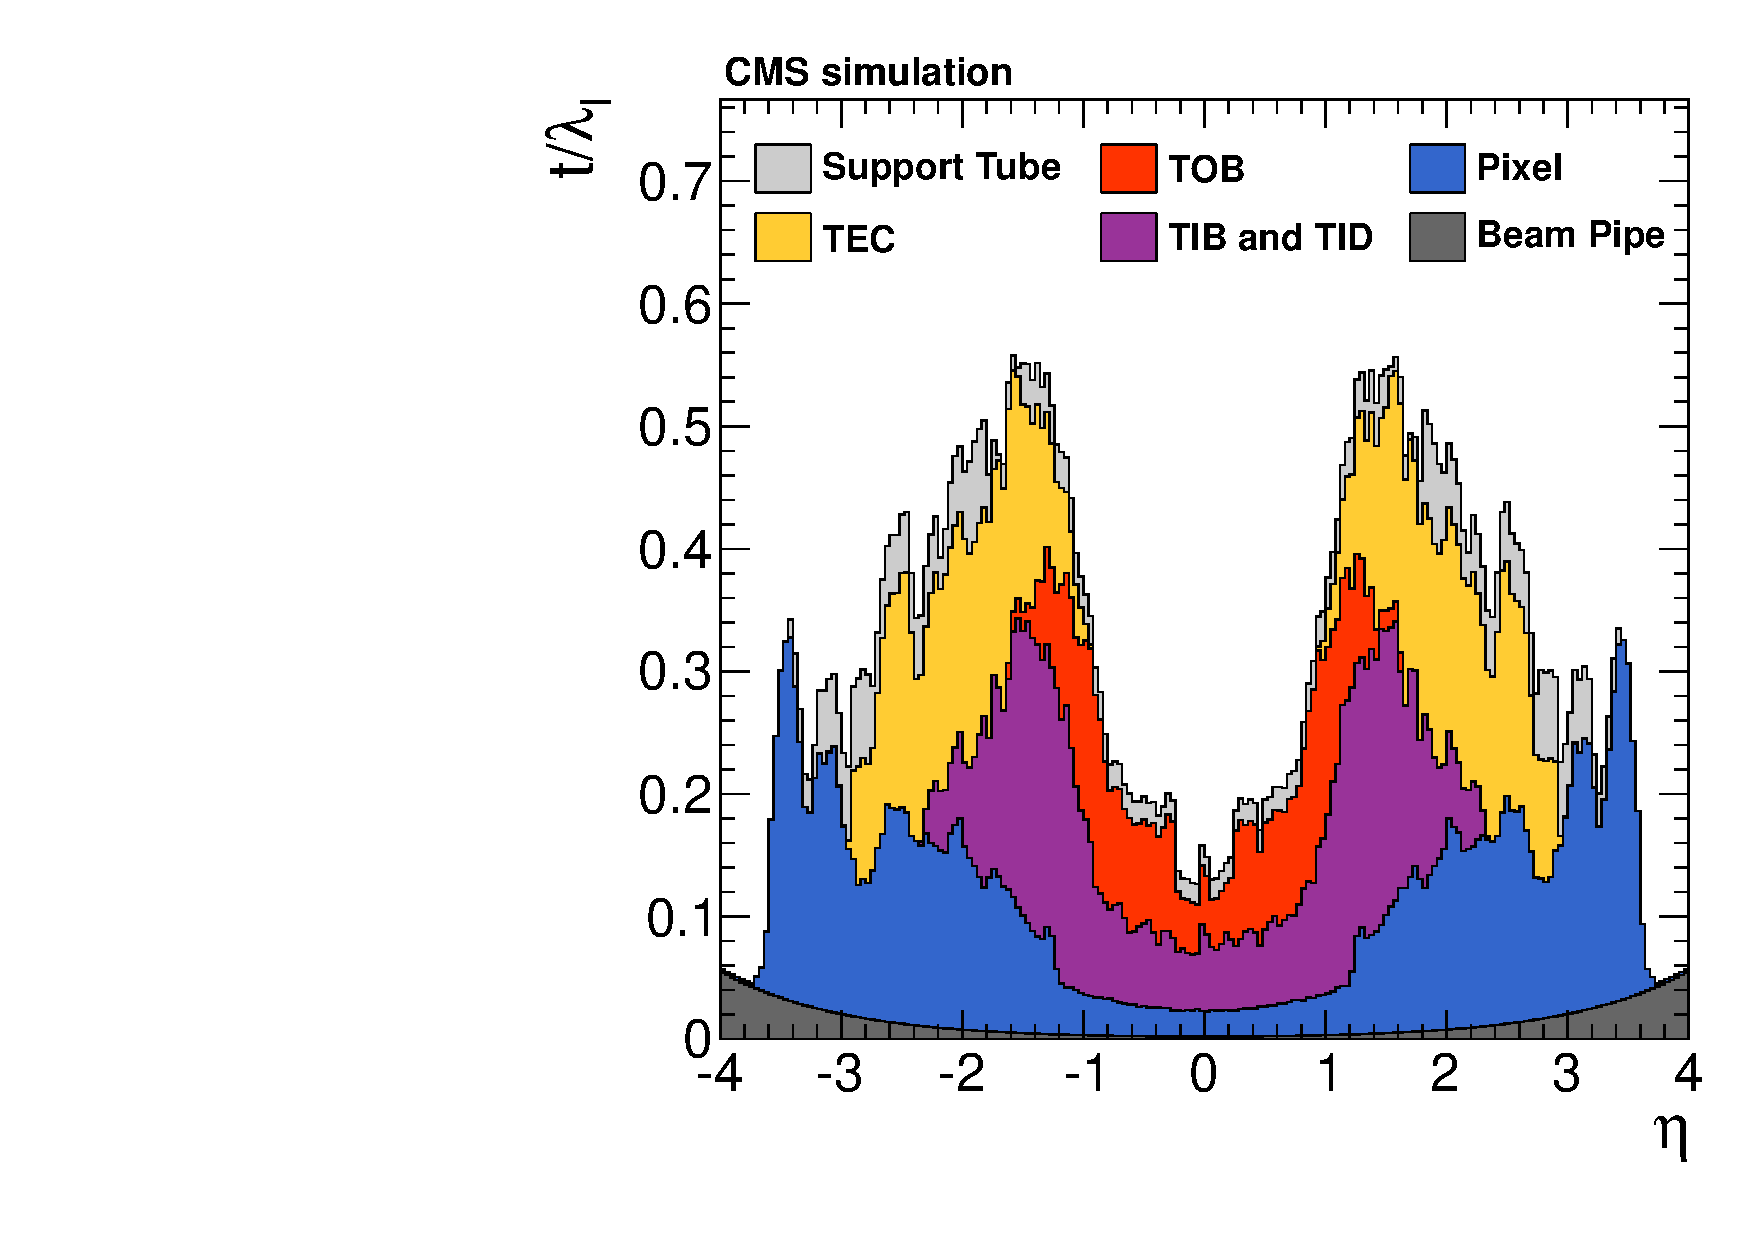
\includegraphics[width=0.4\textwidth]{figures/MaterialBudget_InteractionLengths.pdf}
    \caption[Tracker material budget.]{
      The CMS tracker material budget in (left) radiation lengths (ie electromagnetic) and (right) interaction lengths (ie nuclear), in the configuration used in 2016 and earlier. 
      While the CMS tracker is not intended to shower particles, only to measure positions as gently as possible, some amount of interaction between tracker material and collision products is inevitable.
      Taken from \cite{cmstracking}.}
    \label{fig:trackerbudget}
  \end{figure}  

  \begin{figure}[h!]
    \centering
    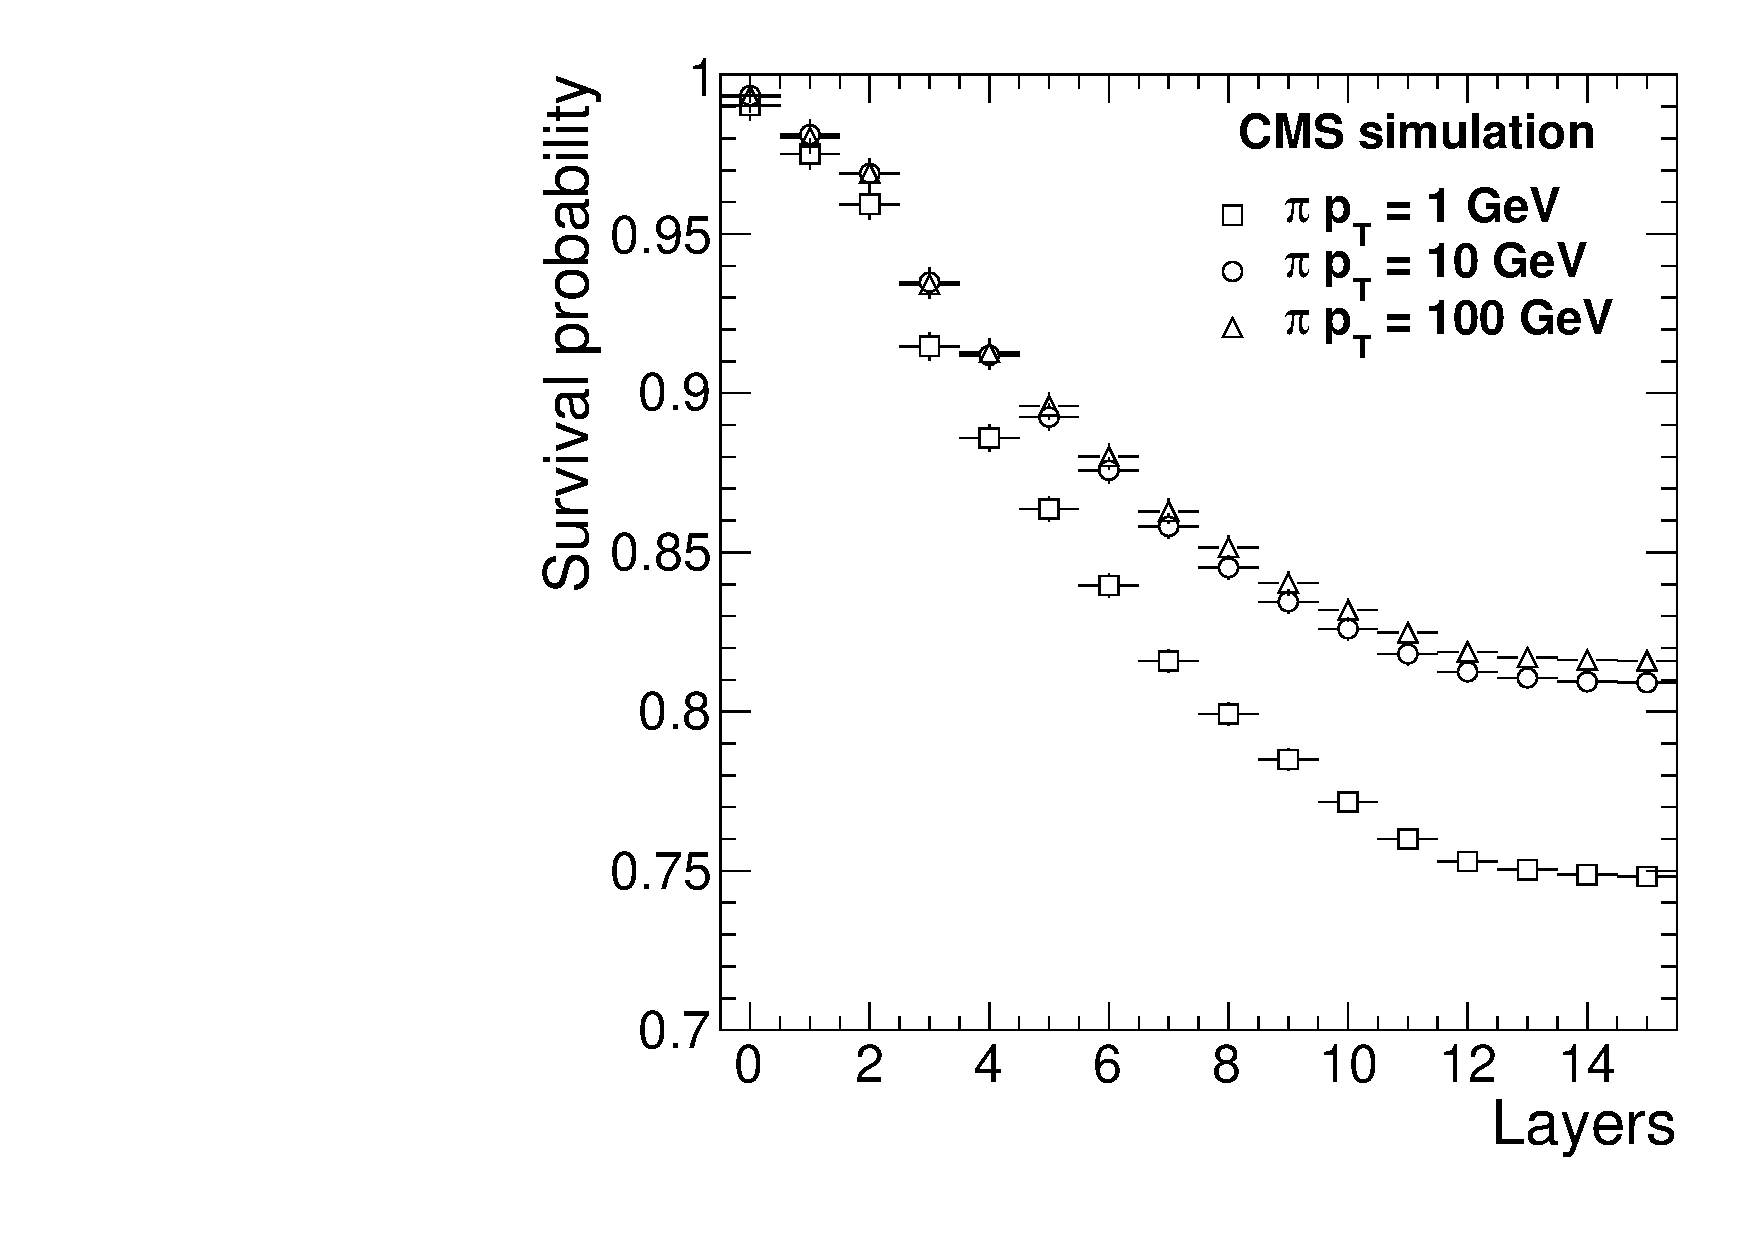
\includegraphics[width=0.85\textwidth]{figures/PionSurvivalProbability.pdf}
    \caption[Pion survival in the tracker.]{
      The probability for pions to undergo nuclear interactions in the CMS tracker by layer, in the configuration used in 2016 and earlier. 
      In rare cases, the pion may shower in such a way that no charged daughters have high enough energy to be reconstructed, causing its track to disappear.
      Taken from \cite{cmstracking}.}
    \label{fig:pionsurvival}
  \end{figure}  

  As a general rule, the tracker intends to interact with particles only to the extent absolutely necessary to measure their positions.
  Strong interactions between the tracker and the particles it is measuring modify the particles' tracks and affect their energies, and are therefore undesirable.
  Unfortunately, electrons are so strongly affected by bremsstrahlung that the tracker is quite thick in terms of radiation lengths, as shown in Figure~\ref{fig:trackerbudget} (left).
  Therefore, electrons at CMS are experimentally observed more as clouds of bremsstrahlung photons by the time they reach the electromagnetic calorimeter at CMS, and must be reconstructed with a special tracking procedure, the Gaussian-sum filter described in \cite{gsftracking}.
  In terms of interaction lengths, the CMS tracker is much thinner, as shown in Figure~\ref{fig:trackerbudget} (right).
  The vast majority of hadrons therefore reach the calorimeters without having undergone a nuclear interaction.
  Figure~\ref{fig:pionsurvival} shows that over 80\% of high energy charged pions reach the calorimeters intact.
  Even so, 80\% is not 100\%.
  Pion tracks occasionally terminate in a shower induced by a collision with a nucleus inside the tracker.
  In rare cases, these showers can contain {\it zero} visible particles of any kind.
  These disappearing pions constitute an important background for the disappearing tracks search.

  \subsection{Electromagnetic Calorimeter} \label{sec:ecal}

  The primary purpose of the electromagnetic calorimeter (ECAL) is to observe the energies of photons, which do not leave tracks.
  It is also important in the observation of electrons, which produce a jet of photons due to bremsstrahlung in the tracker.
  Other electromagnetically interacting particles will also leave small ECAL deposits, but much less due to their lesser tendency to produce photons.
  In Figure~\ref{fig:cmsreconstruction}, the electron (red) and photon (dotted blue) produce strong showers in the ECAL (green), while the other particles leave negligible deposits.

  The design prioritizes good resolution of photon energies and positions over all else, due to the experimental importance of the Higgs boson's decay to a pair of isolated photons.
  To accomplish this, the ECAL is constructed from tens of thousands of scintillating lead tungstate crystals, which has several desirable properties.

  First, these crystals have a Moliere radius of only 2.2~cm \cite{cms_tdr}.
  Aside from providing generally good position resolution, this small Moliere radius most importantly allows a prompt isolated photon, perhaps from a Higgs decay, to be distinguished from two closely overlapping photons produced by the decay of a neutral pion, because the two separate showers produced by the photon pair are clearly separated in the ECAL cells.
  These two nearby showers may merge into a single large shower indistinguishable from that of a single photon in a material with a larger Moliere radius.
  Similarly, photons produced inside jets can be distinguished from truly isolated photons, since the showers of other particles in the jets can be discriminated from the photon's own shower.
  Although the size of the shower is restricted, a typical one will still extend over a few adjacent crystals as shown in Figure~\ref{fig:cmsreconstruction}, so that a 5-by-5 cluster of crystals, or potentially a smeared supercluster for electrons that have radiated over a larger area, is the essential object of ECAL reconstruction.
  Studying the distribution of energy measurements across the crystals in a cluster, as described in \cite{ecal_algorithm}, allows for better fake rejection and energy resolution of 1\% \cite{ecal_energy_resolution}.

  Second, lead tungstate also has an extremely short radiation length, only 0.89~cm compared to the roughly 2 radiation lengths of the entire 1~m radius tracker, so it contains electrons very efficiently \cite{cms_tdr}.

  Third, scintillation in lead tungstate happens quickly, with 80\% of the light produced within 25~ns \cite{cms_tdr}. 
  This speed is critical for coping with the 25~ns bunch spacing of the LHC's proton beams, so that the ECAL deposits produced by adjacent bunch crossings can be distinguished.
  Due to this rapid shower production and careful calibration of the electronics, the ECAL achieves a timing resolution of roughly 0.2~ns for particles with momenta on the order of tens of GeV \cite{ecaltiming}.

  Finally, lead tungstate is resistant to radiation damage, so that the ECAL can continuously operate in the high flux environment of LHC proton collisions.
  Unfortunately, it is not immune to radiation damage, and so the performance of the ECAL degrades over time.
  By the end of data taking in 2018, roughly 20\% of ECAL cells no longer consistently detected showers of photons and electrons.
  This leads to a background for the disappearing tracks search consisting of electrons that transform to photons inside the tracker, no longer leaving a track, but are not later detected as photons in the ECAL.
  Fortunately, 80\% of the ECAL is still performing well despites years of high radiation flux, so this background can be almost entirely rejected by mapping and vetoing the poorly performing cells, using events in which a Z boson decayed to a pair of electrons, exactly one of which is lost due to this effect, as described in Section~\ref{sec:distracks}.

  \subsection{Hadronic Calorimeter} \label{sec:hcal}

  Charged hadrons are too massive to shower significantly in the ECAL, and neutral hadrons are invisible even to the tracker.
  However, both can be made to shower by capitalizing on their powerful nuclear interactions, and the hadronic calorimeter (HCAL) accomplishes this, as depicted in Figure~\ref{fig:cmsreconstruction} for a neutral hadron in dotted green and a charged hadron in solid green.
  The performance of the HCAL is very important to analyses selecting events containing jets and missing energy, as HCAL measurement errors lead directly to errors in jet energies, which in turn cause errors in the inferred missing energy in the event.

  The essential plan of the CMS HCAL design is to induce hadron showers by putting a high density of atomic nuclei in their paths in the form of 5~cm brass plates, then to measure the products of these showers using plastic scintillators, and from this reconstruct the energies of the original hadrons.
  To ensure that as few hadrons as feasible escape detection, whether from the primary interaction or from secondary showers, there are multiple layers of this shower-inducing metal plate and scintillator combination.
  Nevertheless, some hadrons do manage to ``punch through'' the HCAL, especially if they have extremely high energy, and even successful measurements are only accurate to within roughly a factor of 2 \cite{HCALphase1}, unless that hadron has very high energy.
  On the whole, the CMS HCAL performance is the weakest of any detector system.
  However, the energy of a typical jet is not measured only with the HCAL, and errors made on different hadrons within a jet tend to cancel, so that CMS achieves a typical jet energy resolution of approximately 10\%, for the jets of most interest \cite{cms_tdr}.
  Still, jets are occasionally badly mismeasured, most often due to HCAL measurement errors, and it is important for analyses selecting events with large missing energy to filter out these mismeasurement events, see Section~\ref{sec:MT2bg}.

  Accuracy of energy measurements aside, the ability to detect neutral hadrons consistently in the HCAL is important to the disappearing tracks search discussed in Section~\ref{sec:distracks}.
  A charged hadron can decay to a neutral hadron inside the tracker, and thus allow known Standard Model physics to produce an apparent disappearing track.
  Unlike a true disappearing track, however, the neutral hadron is detectable in the HCAL, revealing what happened in the tracker and rejecting this Standard Model background.
  As with the ECAL, poorly performing regions of the HCAL can be vetoed to ensure this background is wholly rejected.

  \subsection{Muon System} \label{sec:muon}

  The muon system is the outermost detector of CMS, and the only one outside the solenoid.
  Muons, like charged hadrons, are too heavy to produce significant showers in the ECAL, and unlike hadrons, do not have nuclear interactions allowing them to be trapped in the HCAL.
  Instead, they penetrate through the entire detector, leaving a track in the tracker, largely disappearing inside the calorimeters, and then reappearing in the muon system.
  Unlike other particles, then, the energies of muons must be measured largely by analyzing the curvature of their tracks.
  As one of the design goals of the Compact Muon Solenoid experiment is ultra-precise measurements of muons, the muon system is large partly in order to provide a long look at the muon's track for momentum measurement purposes, and partly to provide a positive identification of a particle as a muon, rather than a hadron that managed to escape the HCAL, as only muons can penetrate through so many layers of detector material.
  As installing a second tracker would be far too expensive and excessive, the muon system instead uses only four widely spaced layers of detectors operating based on ionization of gas by passing muons, which while generally worse than the tracker system in terms of space and time resolution, are much more economical for covering such a large volume \cite{cms_tdr}.
  The design of CMS has proven successful. 
  Muons are by far the cleanest, most well-measured particles at CMS, with momentum resolution better than 1\% and high efficiency, as we have already seen for tracker muon tracks in Figure~\ref{trackefficiency}.

  While muons are the only charged Standard Model particle that can consistently penetrate to the muon system, the possibility exists that heavy long-lived charged particles beyond the Standard Model may be produced in LHC collisions and leave hits in the muon system.
  The disappearing tracks search in Section~\ref{sec:distracks} targets models that could potentially produce such a signature.
  However, that search considers only tracks that disappear inside the tracker, and in fact explicitly vetoes muon-like tracks, so it is not sensitive to this potential signature.
  Adding sensitivity to this powerful signature could be an interesting extension in the future.

  \subsection{Missing Transverse Energy} \label{sec:MET}

  Once muons are measured in the muon system, all Standard Model particles have been accounted for, except neutrinos.
  Unfortunately, the neutrino interaction length, even at LHC energies, is on the order of billions of meters at Earthly densities, so that the probability of a typical LHC neutrino experiencing even a single interaction anywhere inside the CMS detector is negligible \cite{neutrinos}.
  However, the presence of neutrinos can be inferred by measuring all other particles inside the event, and observing that the transverse momentum does not balance, indicating either the presence of at least one undetected particle, or a detector mismeasurement.
  At a hadron collider like the LHC, only the transverse momentum can be used for this procedure, because the exact center of momentum frame of the primary collision is unknown along the beam axis.
  The actual colliding particles are not the protons themselves, but rather subcomponents of the proton called partons.
  The partons are approximately at rest with respect to the detector in the transverse plane, so that their transverse momenta are known to sum nearly to zero, but have unkonwn momenta along the beam axis.
  Unbalanced momentum along this axis may indicate the presence of an invisible particle, but more often it indicates simply that the initial momentum of the collision along the beam axis was nonzero.
  The observable is not the missing energy, then, but the missing transverse energy, written as MET or \met.
  This observable is tentatively identified with the unobservable transverse momentum of a neutrino.

  Although the invisible momentum is only available in the transverse plane, it is still a very useful quantity.
  For instance, consider the leptonic decay of a W boson, $W^{\pm}\rightarrow\ell^{\pm}\nu$.
  The W boson has mass approximately 80~GeV with width approximately 2 GeV \cite{pdg}.
  Even allowing for detector resolution effects around 10\%, a lepton and neutrino system originating from an on-shell W decay can never have mass greater than approximately 100~GeV.
  It follows directly that transverse mass \Mt, the mass calculated using energy and momentum in the transverse plane, also cannot exceed 100~GeV, since $E_T < E$ and $\pt < p$.
  The analyses discussed in the next Section~\ref{sec:analysis} leverage this fact to determine whether a lepton or disappearing track may potentially have originated in a leptonic W decay.
  
  Of course, while the missing transverse energy is sometimes the undetected energy of a single neutrino or unknown invisible particle, it can also be a consequence of mismeasurement, or even potentially the vector sum of the transverse momenta of {\it multiple} undetected particles.
  In fact, even events with relatively large amounts of missing energy at CMS are most often produced by detector mismeasurement (see Figure~\ref{fig:mt2dist}, in which ``Multijet'' events in yellow have \met due to detector mismeasurement), even though such large errors are rare, because neutrinos are rarer still.
  Searches for invisible particles naturally wish to eliminate these events with fake \met using cleaning selections.
  One of the most powerful observables that can be used to reject events with fake \met is \mttwo \cite{mt2}, a generalization of \Mt.

    \subsubsection{\mttwo} \label{sec:MT2}

    Although the presence of invisible particles can be inferred via the observation of a nonzero \met vector, it is not trivial to distinguish events in which the \met corresponds to the transverse momentum of a single invisible particle, and events in which the \met is the vector sum of the momenta of multiple invisible particles.
    It can also be difficult to distinguish the presence of genuine invisible particles from cases of detector mismeasurement.
    While no conclusions about invisible content can ever be drawn with perfect certainty for any single event, the situation is not hopeless.
    The \mttwo observable is one tool used to make quantitative inferences concerning an event's invisible content.
    Specifically, \mttwo is designed to identify events consistent with the presence of two invisible particles in the final state, produced in symmetric decay chains of pair-produced heavy particles.
    This also tends to reject events in which the \met was produced by detector mismeasurement, as these events tend to have no symmetry whatsoever.

    The algorithm begins by dividing the visible portion of the event into two hemispheres.
    To do this, an event must have at least two visible objects, so in an event with only hadron jets, like the majority of the events at CMS, \mttwo can be calculated only for multijet events.
    The method used to assign each visible object to a hemisphere varies.
    One popular method, and the one used in \cite{MT2_2019}, begins by identifying the pair of objects with largest system mass, $M_{12}$,
    \begin{equation} \label{eqn:dijetmass}
      M_{12} = \sqrt{(E_1+E_2)^2-(\vec{p}_1+\vec{p}_2)^2},
    \end{equation}
    and assigning each as the seed of a separate hemisphere.
    In an event containing two identical pair-produced particles undergoing similar decay chains, the pair of objects with largest mass is unlikely to originate from the same particle, as the mass of the full system is strictly greater than the mass of either particle.

    Then, each object is associated to the seed of lesser Lund distance, $D_{L}$, which is defined for seed $i$ as \cite{lund1,lund2},
    \begin{equation} \label{eqn:lund}
      D_L = (E_{i}-p_{i}\cos\theta)\frac{E_{i}}{(E_{i}+E)^2}
    \end{equation}
    where $E_i$ is the seed's energy, $p_i$ is the seed's momentum, $\theta$ is the angle between the momenta of the seed and of the object under consideration, and $E$ is that object's energy.
    Considering the massless limit of $D_L$ provides some intuition,
    \begin{equation} \label{eqn:lund}
      D_L = \frac{1-\cos\theta}{(1+\frac{E}{E_h})^2}.
    \end{equation}
    The Lund distance is small if the hemisphere and object point in nearly the same direction so that $\cos\theta\sim1$, and if $E_i$ is small.
    Thus, selecting based on minimal Lund distance prefers to assign objects to the less energetic seed when possible to keep the hemispheres energetically balanced, so long as the object and the seed point in similar directions.
    Once all objects have been assigned to a seed, two new seeds are defined as the sum of all the four-momenta in each hemisphere, and the assignment procedure repeats using these seeds.
    This continues until no object changes hemisphere after an iteration.
    Ultimately, the algorithm assigns objects to the correct hemisphere with efficiency ranging from approximately 70--85\%, with higher efficiencies obtained in events with fewer objects and therefore reduced combinatorics \cite{lundeff}.

    The next step of the calculation of \mttwo takes these finalized hemispheres as inputs.
    Under the hypothesis that the observed missing energy is the vector sum of the unobserved momenta of two invisible particles, the algorithm considers every possible vector decomposition,
    \begin{equation}
      \ptvecmiss = \vec{v}_1+\vec{v}_2
    \end{equation}
    and calculates \Mt for hemisphere $i$ with respect to $\vec{v}_i$.
    The maximum of these two values of \Mt is taken as the {\it candidate} \mttwo for this decomposition.
    This choice is motivated by a desire to infer the true mass of the decaying pair-produced particle, again, under the hypothesis that there are two pair-produced particles undergoing symmetric partially invisible decays.
    For the correct \ptvecmiss decomposition and hemisphere assignments, the two calculated transverse masses are correct, and both are no larger than the true mass of the pair-produced particles. 
    The larger, of course, is nearer to that true mass.
    
    The only remaining step is to select which of the candidate values of \mttwo, equivalently which \ptvecmiss decomposition, is correct.
    The algorithm selects the smallest candidate \mttwo value found, the ``minimum maximum,'' so that the final \mttwo is
    \begin{equation} \label{eqn:minmax}
      \mttwo = \underset{\ptvecmiss = \vec{v}_1+\vec{v}_2}{\min}\left[\max\left(\Mt^1,\Mt^2\right)\right]
    \end{equation}
    where hemispheres 1 and 2 are assembled as described above.
    Since the correct missing energy decomposition is among those considered and manifestly cannot produce a value of \Mt greater than the true mass of the parent particle when hemisphere assignments are correct, selecting the ``minimum maximum'' guarantees that \mttwo can be no larger than the mass of the parent particle. 
    Just as \Mt cannot exceed the mass, \mttwo is unlikely to exceed the true \Mt.

    Of course, it is possible for \mttwo to be small even in genuine signal events for which it is designed to be large, and it is possible for especially pathological mismeasurement events to have large \mttwo despite \mttwo being a powerful rejector of these backgrounds (see Section~\ref{sec:MT2QCD}).
    No observable is so magical that it can accept 100\% of signal and reject 100\% of background.
    Still, \mttwo is one of the most powerful discriminants available for analyses targeting pair-produced particles decaying semi-invisibly, as can be seen for instance in Figure~\ref{fig:mt2dist}.
    Indeed, the selection of $\mttwo > 200$~GeV applied by the analyses discussed in Section~\ref{sec:analysis} is the single most important part of their baseline selection, dramatically reducing especially the detector mismeasurement background.

\section{CMS Event Reconstruction} \label{sec:reconstruction}

  \subsection{Challenges} \label{sec:challenges}

  Spray of thousands of particles, many in dense jets, from collisions distributed across a rather large beam crossing, millions of times per second.
  Pace is so high that travel of electrical impulses along the equipment is comparable to the collision frequency.

    \subsubsection{The Trigger System} \label{sec:trigger}

    High event rate needs to be suppressed due to computing limitations.
    High event rate is necessary to see rare things (how rare?).

    \subsubsection{Pileup} \label{sec:pileup}

    Obtaining a high enough event leads to many simultaneous collisions (not 1 proton collision at a time, but bunches crossing every 25 ns).
    Charged pileup contribution can be subtracted exactly using the tracker, but neutral pileup correction is heuristic.
    Effective area vs delta-beta.

    \begin{figure}[h!]
      \centering
      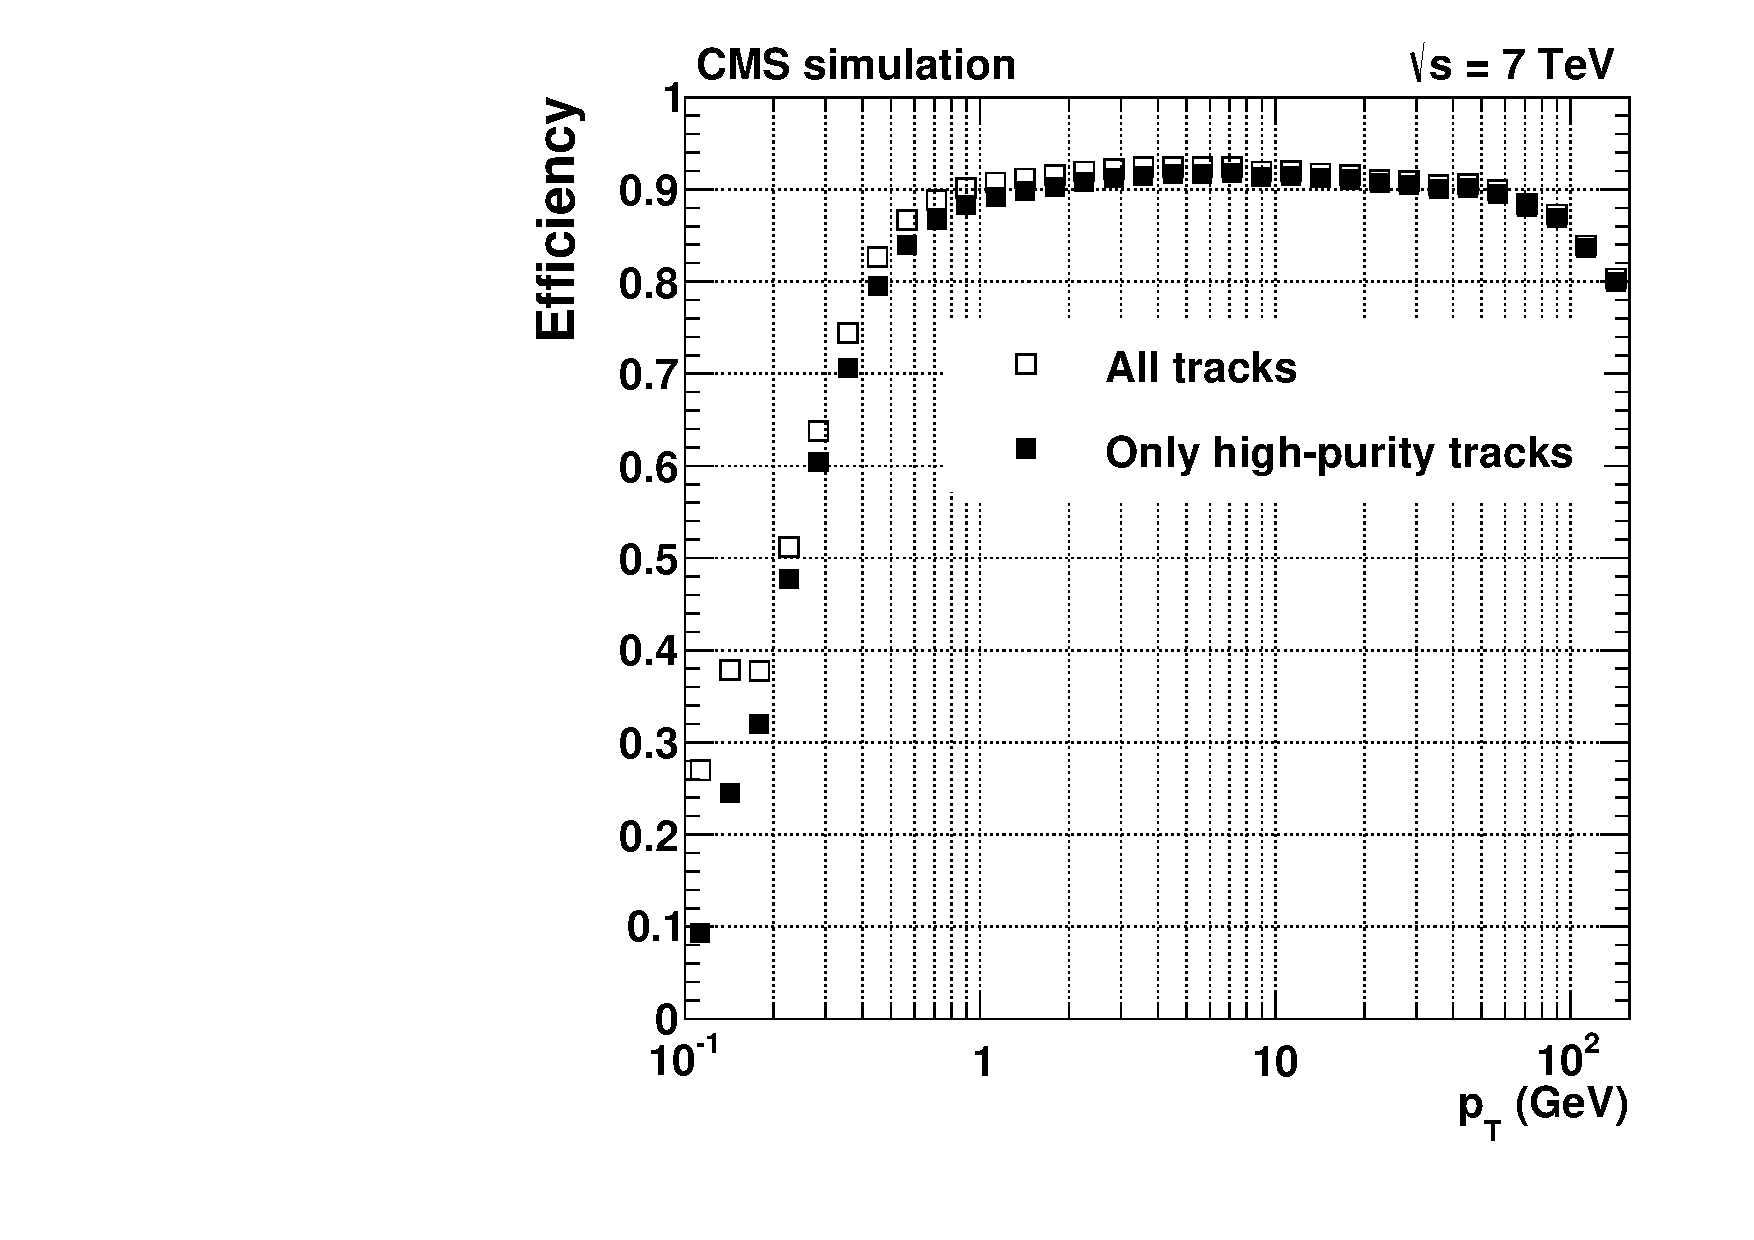
\includegraphics[width=0.65\textwidth]{figures/efficiencyVsPt.pdf}
      \caption[Pileup distribution in 2018.]{
        The distribution in 2018 of the number of simultaneous collisions per bunch crossing, so-called pileup, provided by the LHC and observed by CMS.
        The average bunch crossing produced 32 simultaneous collisions, with an inferred total inelastic collision cross section of 69.2~mb.
        Taken from \cite{lumipublic}.}
      \label{fig:pileup}
    \end{figure}  

  \subsection{Vertices} \label{sec:vertices}

  Use tracker to identify tracks and extrapolate them back to an origin point.
  These origins are vertices.

    \subsubsection{B-Tagging} \label{sec:btagging}

    Some tracks will not extrapolate back to a proton collision point but instead a point a few millimeters away: secondary vertices characteristic of b-tags.
    Describe other indicators used to identify b-jets and the efficiency.

  \subsection{Particle Flow} \label{sec:particleflow}

  Describe particle flow algorithm and advantage relative to other techniques.

  \subsection{Jet Clustering} \label{sec:jetclustering}

  Jets are made from PF candidates using anti-kt.
  How accurately?

\section{Simulation} \label{sec:simulation}

  The Standard Model and models of new physics predict what happens at the primary interaction, and this needs to be converted into a prediction for what happens in the detector.

  \section{Objectives} \label{sec:objectives}

  Used to study backgrounds and develop estimation techniques, and to design analyses to maximize sensitivity to expected signal signatures.

  \section{Limitations and Challenges} \label{sec:limitations}

  Ultra-detailed knowledge of the detector at the subatomic level at all locations is unachievable, and the detector's state evolves over time.
  QCD is irritating, and even electroweak physics is subject to theoretical uncertainties due partly to dependence on experimental inputs, and partly to calculating only to finite order.
  Can't run the simulation forever, and the computation is expensive.

  \section{The Simulation Pipeline} \label{sec:pipeline}

  Matrix elements (MadGraph), observed particles (pythia), how those particles interact with detector components (GEANT).
  Mention also fastsim vs fullsim (ie replacing GEANT with approximate smearing).

  \chapter{The Full 13 TeV \mttwo Analysis} \label{sec:analysis}

This section presents two searches for new physics in all-hadronic final states with substantial \met as inferred through large \mttwo in 13 TeV proton-proton collisions recorded by the CMS detector \cite{MT2_2019}.

The \met selection targets invisible particles, motivated by the evidence for dark matter discussed in Section \ref{sec:DMevidence}.
If dark matter is at least partially composed of a particle or particles associated with physics at the weak scale, then it may be produced in LHC collisions and, while not detectable itself, be inferred via an excess of events with imbalanced transverse momentum.

Considering only all-hadronic events with large \mttwo is part of a divide and conquer strategy employed by the CMS collaboration.
CMS analyses also search for dark matter in events containing leptons, e.g. \cite{cms1lep}, but there is no way to know whether dark matter will be found in either or both.
By splitting the searches, each can optimize for its unique event characteristics.
Likewise, the collaboration also considers all-hadronic events that do not necessarily have large \mttwo \cite{ra2b}, since while \mttwo in many cases provides enhanced sensitivity, it can reduce sensitivity to some models, for instance in cases where the decay energy is very small, or those in which invisible particles are not produced in pairs.

The first search is inclusive, and is a continuation of previous analyses based on smaller datasets, most recently using the 35.9 \fbinv dataset recorded in 2016 \cite{MT2_2016}.
Accordingly, it is referred to as the classic search.

The second search is a new extension of the first, requiring additionally the presence of a disappearing track in a selected event.
Disappearing tracks have been targeted as an observable of interest by both CMS \cite{cmsdistracks_8tev, cmsdistracks_13tev} and ATLAS \cite{atlasdistracks_8tev, atlasdistracks_13tev} previously, but with lower energy or smaller datasets, and different methods.

Both searches set the strongest constraints to date on a variety of hypothetical extensions to the Standard Model possessing pair-produced dark matter candidates, most notably R-parity conserving supersymmetry.

\section{Classic Search} \label{sec:MT2classic}

  \subsection{General Description} \label{sec:classicdescription}

  The classic search's core, defining selections are for events with large missing transverse energy \met as inferred via \mttwo, large total hadronic transverse energy, called \Ht, and no leptons.

  The primary motivation for the analysis is either finding or setting constraints on particle dark matter.
  The experimental signature of dark matter is its undetectability; its presence can only be inferred through large imbalance of transverse energy.
  The \mttwo analysis further focusses on the case of pair-produced dark matter using its eponymous observable.
  For reasons discussed in Section \ref{sec:SUSY}, R-parity conserving supersymmetry is a model of special interest to the theoretical community, and this model's dark matter candidate would always appear in pairs.
  The \mttwo variable tends to increase sensitivity to the pair-production scenario as described in Section~\ref{sec:MT2}.

  The selection of events with large \Ht is motivated by the CMS trigger as discussed in Section \ref{sec:trigger}, which is in turn motivated by the inferred large energy scale of new physics.
  The decays of heavy new particles to relatively light Standard Model particles will result in, typically, very energetic events.
  It is possible that the dark matter candidate is itself very heavy, nearly as massive as the new particle that decays to it.
  In this scenario, while the events are indeed very energetic, much of the energy is lost to the invisible portion of the event, and the visible, hadronic energy can be relatively small.
  Accordingly, sensitivity in the compressed scenario is weaker, as many of the new physics events are too low energy to pass the kinematic selections.
  The \mttwo selection is especially inefficient, in this scenario.
  However, sensitivity is not negligible, and the search is sensitive to any mass splitting in many cases.
  
  The last selection, a veto of leptons, is chiefly motivated by CMS's divide and conquer strategy.
  Final states including leptons are considered in other searches.
  However, the veto does allow for partial suppression of the Standard Model neutrino background, since neutrinos are often produced alongside a charged lepton in decays of the W boson, as discussed in Section \ref{sec:MT2bg}.

  Ideally, any observation of an event with large \met and \mttwo, large \Ht, and no leptons, would constitute a discovery.
  Unfortunately, this is not the case, as the Standard Model is capable of producing events with all of these signatures.
  Neutrinos and simple mismeasurement of the event can produce large missing energy signatures, events with large \Ht are uncommon in the Standard Model but hardly impossible, and the vast majority of events in a proton-proton collider have no leptons.
  Some number of events will have all of these properties without any new physics occurring, and most of the analysis' efforts are spent estimating how often these background processes occur, as discussed in Section \ref{sec:MT2bg}.

  \subsection{Signals} \label{sec:MT2sig}

  \begin{figure}[h!]
    \centering
    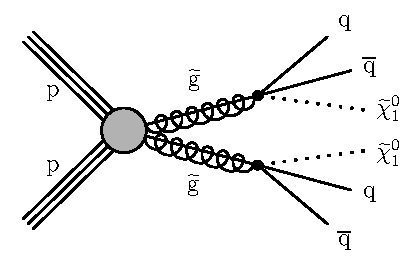
\includegraphics[width=0.3\textwidth]{figures/MT2_2019/Figure_007-a}
    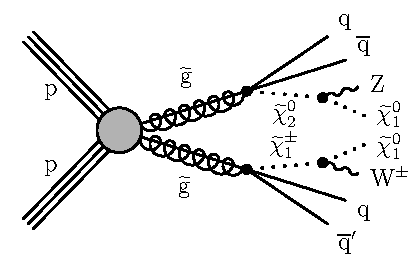
\includegraphics[width=0.3\textwidth]{figures/MT2_2019/Figure_007-b}
    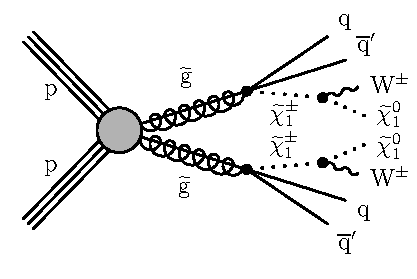
\includegraphics[width=0.3\textwidth]{figures/MT2_2019/Figure_007-c}\\
    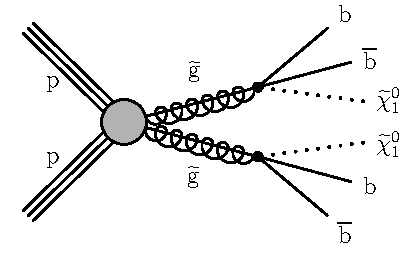
\includegraphics[width=0.3\textwidth]{figures/MT2_2019/Figure_007-d}
    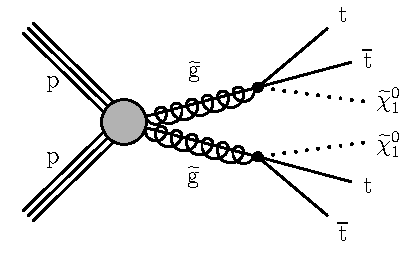
\includegraphics[width=0.3\textwidth]{figures/MT2_2019/Figure_007-e} \\
    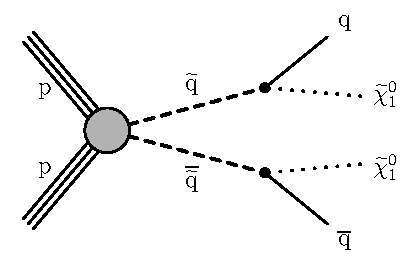
\includegraphics[width=0.3\textwidth]{figures/MT2_2019/Figure_007-f}
    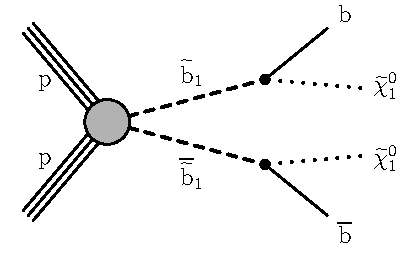
\includegraphics[width=0.3\textwidth]{figures/MT2_2019/Figure_007-g}
    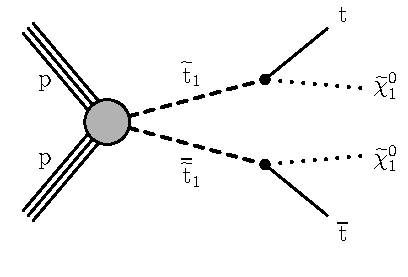
\includegraphics[width=0.3\textwidth]{figures/MT2_2019/Figure_007-h} \\
    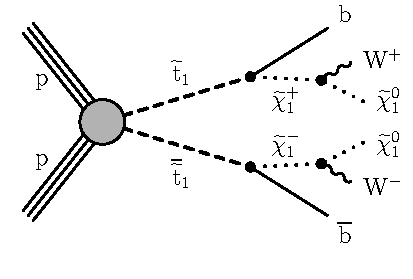
\includegraphics[width=0.3\textwidth]{figures/MT2_2019/Figure_007-i}
    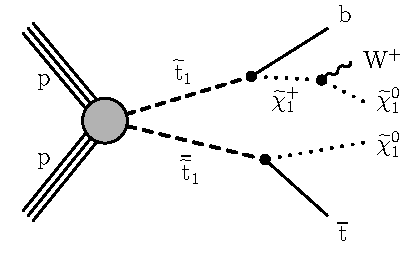
\includegraphics[width=0.3\textwidth]{figures/MT2_2019/Figure_007-j}
    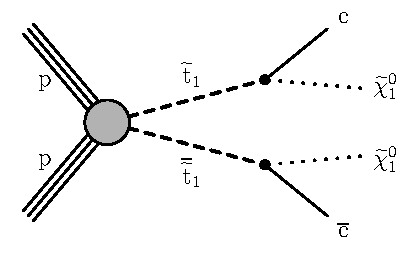
\includegraphics[width=0.3\textwidth]{figures/MT2_2019/Figure_007-k} \\
    \caption[Diagrams for gluino and squark pair production, as predicted by supersymmetric extensions of the Standard Model.]{Diagrams of gluino (upper five) and squark (lower six) pair production, as predicted by supersymmetric extensions of the Standard Model. 
The classic search considers five potential gluino decay chains. 
At upper left, the gluinos decay to light flavor quarks (up, down, strange, or charm), and the lightest neutralino, \lsp.
At upper center, the gluinos decay to light flavor quarks, but rather than decaying directly to \lsp, the gluinos decay either to the second neutralino, \chitwo, which subsequently decays to a Z boson and \lsp, or to the lightest chargino, \chargino, which subsequently decays to the W boson and \lsp, with equal probability.
At upper right, both gluinos undergo the \chargino to W decay chain.
On the left of the second row, both gluinos decay to bottom quark pairs and \lsp.
On the right of the second row, both gluinos decay to top quark pairs and \lsp.
Additionally, the classic search considers six potential modes of squark production and decay.
On the left of the third row, light flavor squarks decay to light flavor quarks and \lsp.
In the center of the third row, bottom squarks decay to bottom quarks and \lsp.
On the right of the third row, top squarks decay to top quarks and \lsp.
At lower left, top quarks decay to bottom squarks and \chargino, which subsequently decay to the W boson and \lsp.
At lower center, top squarks may undergo either the \chargino decay chain, or a direct decay to a bottom squark and \lsp, with equal probability.
At lower right, each top squark decays to a charm squark and \lsp.
Taken from \cite{MT2_2019}.}
    \label{fig:susyproduction}
  \end{figure}  

    The classic search generically targets any new physics that produces high \Ht events with jets and missing energy from undetected particles.
    Diagrams for several candidate models are shown in Figures~\ref{fig:susyproduction}, \ref{fig:monophidiag}, and \ref{fig:LQdiags}.
    The diagrams in Figure~\ref{fig:susyproduction} of gluino and squark pair production as predicted by supersymmetric extensions of the Standard Model are of greatest interest, and while the analysis is sensitive to a wide variety of similar hypothetical models, it is optimized for these.
    As discussed in Section \ref{sec:SUSYsms}, these models simplify the enormous parameter space of supersymmetric extensions by assuming that all superpartners except those in the process are so massive that they can be neglected entirely.
    The upper five diagrams all depict pair production of gluinos, $\tilde{g}$, the supersymmetric partner of the gluon.
    As each gluino decays to two quarks, each of which will typically produce a jet, gluino pair production events tend to have many jets.
    Many different decay chains are possible, and the analysis considers five representative benchmarks.

    In the first benchmark, the gluinos decay to light flavor quarks (up, down, strange, or charm), and the lightest neutralino, \lsp.

    In the second benchmark, the gluinos decay to light flavor quarks, but rather than decaying directly to \lsp, the gluinos can decay either to the second neutralino, \chitwo, which subsequently decays to a Z boson and \lsp, or to the lightest chargino, \chargino, which subsequently decays to the W boson and \lsp.
    Each of these decays can occur with equal probability.
    Both the W and Z will themselves decay, usually to a pair of quarks, which will in turn produce jets. 
    So, relative to the first signal model, the second tends to have greater jet multiplicity.
    The Z can also decay to neutrinos, and the W can decay to a neutrino and a lepton that is not reconstructed.
    In these scenarios, this benchmark trades some jets for an enhanced missing energy signature.
    If  the W or Z decays leptonically and a lepton is successfully reconstructed, events from these signals may fail the lepton veto and instead end up in control regions, biasing the background prediction.
    The procedure used to handle such signal contamination of control regions is described in Section \ref{sec:MT2sigcontam}.

    The third benchmark, in which both gluinos undergo the \chargino to W decay chain, is similar.

    In the fourth benchmark, both gluinos decay to the bottom quark and \lsp.
    As described in Section \ref{sec:btagging}, it is possible to identify jets that originated from a bottom quark; such a jet is said to be ``b-tagged.''
    The classic search bins in the number of b-tagged jets in order to enhance sensitivity to signals of this type.

    In the fifth and final gluino pair-production benchmark, both gluinos decay to top quarks and \lsp.
    The top quark decays with probability near unity to a bottom quark and a W boson.
    The extra W bosons, compared to the direct bottom decay model, can either add jets or leptons and neutrinos, as previously discussed.
    This signal tends to produce the most remarkable events of any signal model considered, with very large \Ht, \njet, and \nb, but also loses many events to the lepton veto as any of the four W bosons is liable to produce a lepton.

    The lower six diagrams of Figure~\ref{fig:susyproduction} all depict pair production of squarks, the supersymmetric partners of quarks.
    Squark decays directly produce only one quark each, compared to two for gluino decays, so squark pair-production events tend to have fewer jets than gluino pair-production events.

    In the first squark benchmark diagram, on the left of the third row, a pair of light flavor squarks (up, down, strange, or charm) is produced and each decays to a light flavor squark and \lsp.
   
    In the second benchmark, bottom squarks are produced and decay to bottom quarks and \lsp.
    These events tend to have b-tagged jets, but fewer than in gluino decays to bottom squarks.

    In the third benchmark, top squarks are pair produced and decay to top quarks and \lsp.
    The relationship between this process and the previous one is similar to the relationship between the fifth and fourth gluino benchmarks, respectively.

    The fourth benchmark is very similar to the third.
    Instead of the top squark decaying directly to a top quark, which then decays to a bottom quark and W boson, the squark decays to a bottom quark directly and \chargino, which subsequently produces the W.
    While the final state particles are identical, their kinematics can be very different depending on the distribution of masses realized in nature.
    For instance, if the top squark and \chargino mass splitting is very small, the bottom quark jet in this benchmark may have such low \pt in a typical event that it is difficult to reconstruct.

    In the fifth benchmark, each top squark may undergo the \chargino decay chain or decay directly to a bottom squark and \lsp, with equal probability, mixing the two previous models.

    In the last benchmark, each top squark decays to a charm quark and \lsp.
    This decay chain could dominate when the top squark and \lsp mass splitting is too small to allow decay to on-shell top quarks, and the mass of \chargino is larger than that of the top squark.

    In each of these models, the mass of the squark or gluino and the mass of \lsp are free parameters.
    Large squark and gluino masses cause low production rates, as the production cross sections drop rapidly with increasing mass, as discussed in Section \ref{sec:SUSYsms} and shown in Figure~\ref{fig:SUSYxsec}.
    The mass of \lsp does not affect the production rate, but it does affect the character of the events.
    When the mass splitting between the gluino or squark and \lsp is small, only a small portion of the event's energy ends up in the visible decay products, and most is lost to the rest energy of \lsp.
    These events have low \Ht and \met, low \njet, and when applicable, low \nb, and more closely resemble background.
    As the mass splitting increases, more energy shifts to the visible portion of the event, making events less background-like and increasing sensitivity.
    The analysis considers a grid of potential mass points for each model, and this sensitivity pattern is evident in the curves shown in Section \ref{sec:MT2limits}.
    
    The classic search also considers non-supersymmetric models.

    The first is referred to as the mono-$\phi$ model.
    In this model, a colored boson much like a squark is produced singly, rather than pair-produced as mandated in squark models to conserve R-parity, and decays to a quark and invisible fermion, as shown in Figure~\ref{fig:monophidiag}.
    This model has an especially low number of jets and low \mttwo, and so would appear in more background-like bins than most supersymmetric models.
    In fact, it was originally proposed \cite{monophi} to explain a potential excess in bins of this sort in the previous edition of the classic search, published based on 2016 data \cite{MT2_2016}, and so there is some interest in whether such an excess persists in the larger dataset.
    While the analysis is not optimized for this kind of model, it still has some residual sensitivity to any model characterized by jets and missing energy in the final state, including mono-$\phi$.

    The second non-supersymmetric model, and final model considered explicitly by the classic search, is a leptoquark extension of the Standard Model.
    As discussed in Section \ref{sec:othermodels}, while squarks can decay to a quark and \lsp, leptoquarks can decay to a quark and a neutrino.
    A neutrino is experimentally effectively indistinguishable from a low mass \lsp, such that leptoquarks and squarks produce nearly identical final states, as first established in a reinterpretation of the 2016 edition of the classic search \cite{LQ2016}.
    Thus, it is a relatively simple exercise to reinterpret squark results in the low mass \lsp limit as leptoquark results.
    A few leptoquark production diagrams are shown in Figure~\ref{fig:LQdiags}.

  \begin{figure}[h!]
    \centering
    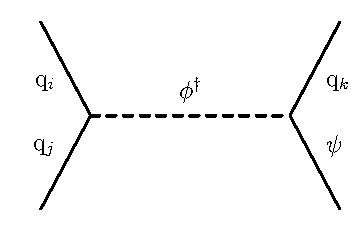
\includegraphics[width=0.85\textwidth]{figures/MT2_2019/Figure_008.pdf}
    \caption[Diagram for the mono-$\phi$ model.]{Diagram for the mono-$\phi$ model, in which a colored scalar $\phi$ is resonantly produced, and decays to an invisible massive Dirac fermion $\psi$ and an SM quark. Note that $\phi$ is not pair-produced, in contrast to otherwise-similar squarks. Taken from \cite{MT2_2019}.}
    \label{fig:monophidiag}
  \end{figure}  

  \begin{figure}[h!]
    \centering
    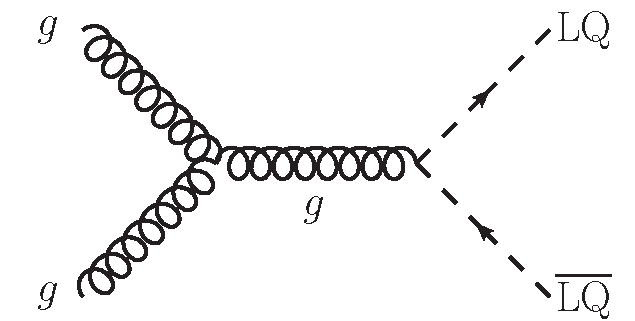
\includegraphics[width=0.3\textwidth]{figures/MT2_2019/Figure_009-a}
    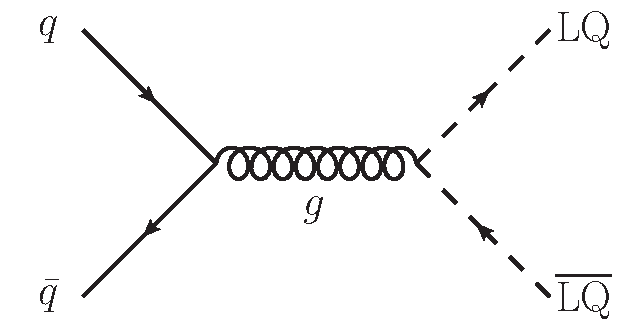
\includegraphics[width=0.3\textwidth]{figures/MT2_2019/Figure_009-b}\\
    \vspace{3mm}
    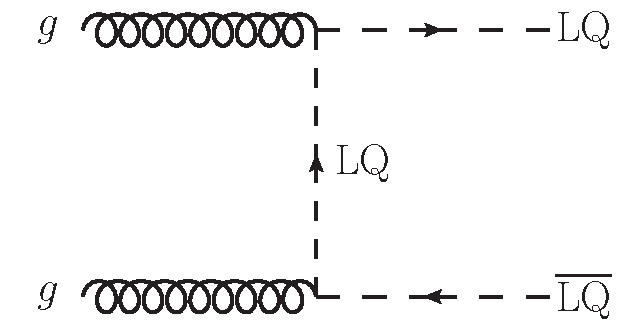
\includegraphics[width=0.3\textwidth]{figures/MT2_2019/Figure_009-c}
    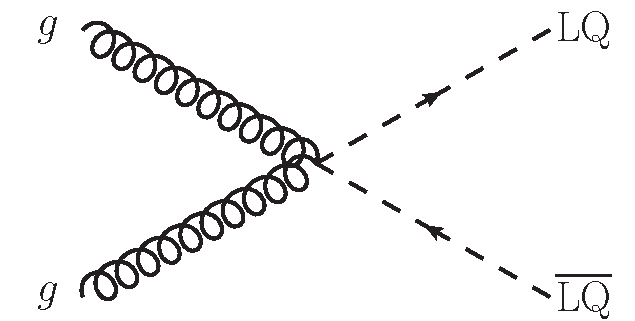
\includegraphics[width=0.3\textwidth]{figures/MT2_2019/Figure_009-d}
    \vspace{3mm}
    \caption[Leptoquark pair production diagrams.]{Diagrams of leptoquark pair production. Each lepqtoquark decays to a neutrino and a quark. Taken from \cite{MT2_2019}.}
    \label{fig:LQdiags}
  \end{figure}  

  \begin{table}[htb]
    \topcaption[Table of systematic uncertainties affecting expected signal yields.]{
      Systematic uncertainties in the signal yields for the simplified models of BSM physics.
      The large statistical uncertainties in the simulated signal sample come from a small number of bins with low acceptance,
      which are typically not among the most sensitive bins contributing to a given model benchmark point.
      Taken from \cite{MT2_2019}.
      \label{tab:sig_systs}}
    \centering
    \begin{tabular}{lc}
      \hline
      Source & Range [\%] \\
      \hline
      Integrated luminosity                     & 2.3--2.5     \\
      Limited size of MC samples                & 1--100  \\
      $b$-tagging efficiency, heavy flavors       & 0--40   \\
      $b$-tagging efficiency, light flavors       & 0--20   \\
      Lepton efficiency                         & 0--20   \\
      Jet energy scale                          & 5       \\
      Fast simulation \met modeling            & 0--5     \\
      ISR modeling                              & 0--30   \\
      $\mu_{\mathrm{R}}$ and $\mu_{\mathrm{F}}$  & 5       \\
      \hline
    \end{tabular}
  \end{table}
  By necessity and unlike backgrounds, the expected event yields for signal models are obtained directly from simulation.
  For this reason, while most uncertainties are shared with background, signal estimates are exposed to a few extra uncertainties, and some of the shared uncertainties increase in magnitude.

  First, while background is normalized to control region counts and so automatically scaled to the correct integrated luminosity, signal counts must be scaled by an independent measurement of the integrated luminosity.
  This measurement is only precise to within a few per cent, leading to a few per cent uncertainty on the expected event count.

  Second, additional jets obtained from ISR must be modeled in simulation for signal, while for background, the control regions provide a precise measurement of the relevant ISR jet production.
  In bins with many jets, where ISR jet production rates are less well-known and simultaneously more important, this uncertainty is as large as 30\%.

  Finally, signal models must be simulated in the fast-simulation framework discussed in Section~\ref{sec:limitations} to make the enormous array of signal scenarios considered computationally feasible.
  A systematic is assessed to cover potential errors made by this approximation.

  The remaining uncertainties are described in the next section, in the context of background estimates.

  \subsection{Backgrounds} \label{sec:MT2bg}

  All of the targeted signals are characterized by all-hadronic events with large missing energy, but observing such an event does not constitute discovery due to the existence of backgrounds that can produce the same basic signature.
  These backgrounds can be broadly divided into the detector mismeasurement background, in which apparent missing energy is generated not by genuine undetected particles but by an error in reconstruction, and the neutrino background, in which the missing energy is produced by genuine neutrinos as predicted in the Standard Model.
  The neutrino background can be subdivided into neutrinos originating from $W^{\pm}\rightarrow \ell^{\pm}\nu$, in which the presence of a charged lepton allows the neutrino to be rejected with good efficiency, and those originating from $Z\rightarrow \nu\nu$, in which the final state is entirely invisible and cannot be efficiently vetoed.

  
    \subsubsection{Mismeasurement} \label{sec:MT2QCD}
  
    The most problematic background is that caused by detector mismeasurement.
    Nearly every mismeasured event is a QCD multijet event, because nearly every event at a proton-proton collider is a QCD multijet event and the probability of mismeasurement is roughly flat across events. 
    Accordingly, the mismeasurement background is also referred to as the QCD multijet background.
    While the detector makes mistakes only very rarely, QCD events are so relatively common that this background is still dominant in the raw dataset, before any cleaning selections.

    Estimating the QCD background is challenging because it requires highly detailed knowledge of the detector's idiosyncrasies.
    Rather than risk falsely discovering a signal or failing to identify one that is present due to misprediction of this background, the analysis adopts selections designed to suppress it, until the background is sufficiently minor that large relative error in its prediction is acceptable.
    
    The first and most powerful of these selections uses the \mttwo variable described in Section \ref{sec:MT2}, namely $\mttwo > 200$~GeV, where the value is chosen to achieve the desired suppression of the mismeasurement background.
    Although the \mttwo selection is somewhat expensive in the sense that it eliminates a significant fraction of signal, especially for signals with a small mass splitting and signals like mono-$\phi$ that are not pair-produced, it is crucial for suppressing the mismeasurement background.
    At $\Ht > 1500$~GeV, the mismeasurement background extends unacceptably beyond $\mttwo \sim 200$~GeV, and the \mttwo selection is tightened to $\mttwo > 400$~GeV.

    The second selection uses the observable 
    $$\dphimin = \textrm{Min}\left(\left|\phi_{\met}-\phi_i\right|\right)$$
    where $\phi_i$ indicates the $\phi$ coordinate of the $i$th \pt jet and $\phi_{\met}$ is the $\phi$ coordinate of the missing energy vector.
    Stated simply, \dphimin\, is the smallest angular separation in the transverse plane of the missing energy vector and any of the four highest \pt jets.
    Close overlap between a jet and the missing energy vector indicates a high probability that the jet was badly mismeasured, and that this mismeasurement is the source of \met in the event.
    The selection applied is $\dphimin > 0.3$, where the value is chosen to achieve strong background rejection without too great a loss of signal efficiency.
    Only the four highest energy jets are used because the probability of {\it some} jet overlapping the missing energy vector approaches unity as the number of jets increases, so the selection would nearly always veto high \njet\xspace events, and the high \njet\xspace bins are sufficiently background-depleted that aggressive background rejection is not as necessary.
    The effect of this selection is depicted in Figure~\ref{fig:dphimin}, after an \mttwo selection of only 100 GeV.

    The last selection rejects events in which a suspiciously large fraction of the missing energy comes from very soft objects.
    The minimum \pt for selected jets is 30~GeV.
    The missing energy vector from only selected jets is denoted $\vec{\HTm}$.
    The missing energy vector used in the analysis, $\vec{\met}$, uses all PF candidates, including those outside jets or in jets with $\pt < 30$~GeV.
    If these two quantities are very different, it means that a large portion of the \met in the event was generated by these low \pt objects, a sign that something may have gone wrong in reconstruction.
    Specifically, the selection is $\left|\vec{\HTm}-\vec{\met}\right|/\met < 0.5$.

    \begin{figure}[h!]
      \centering
      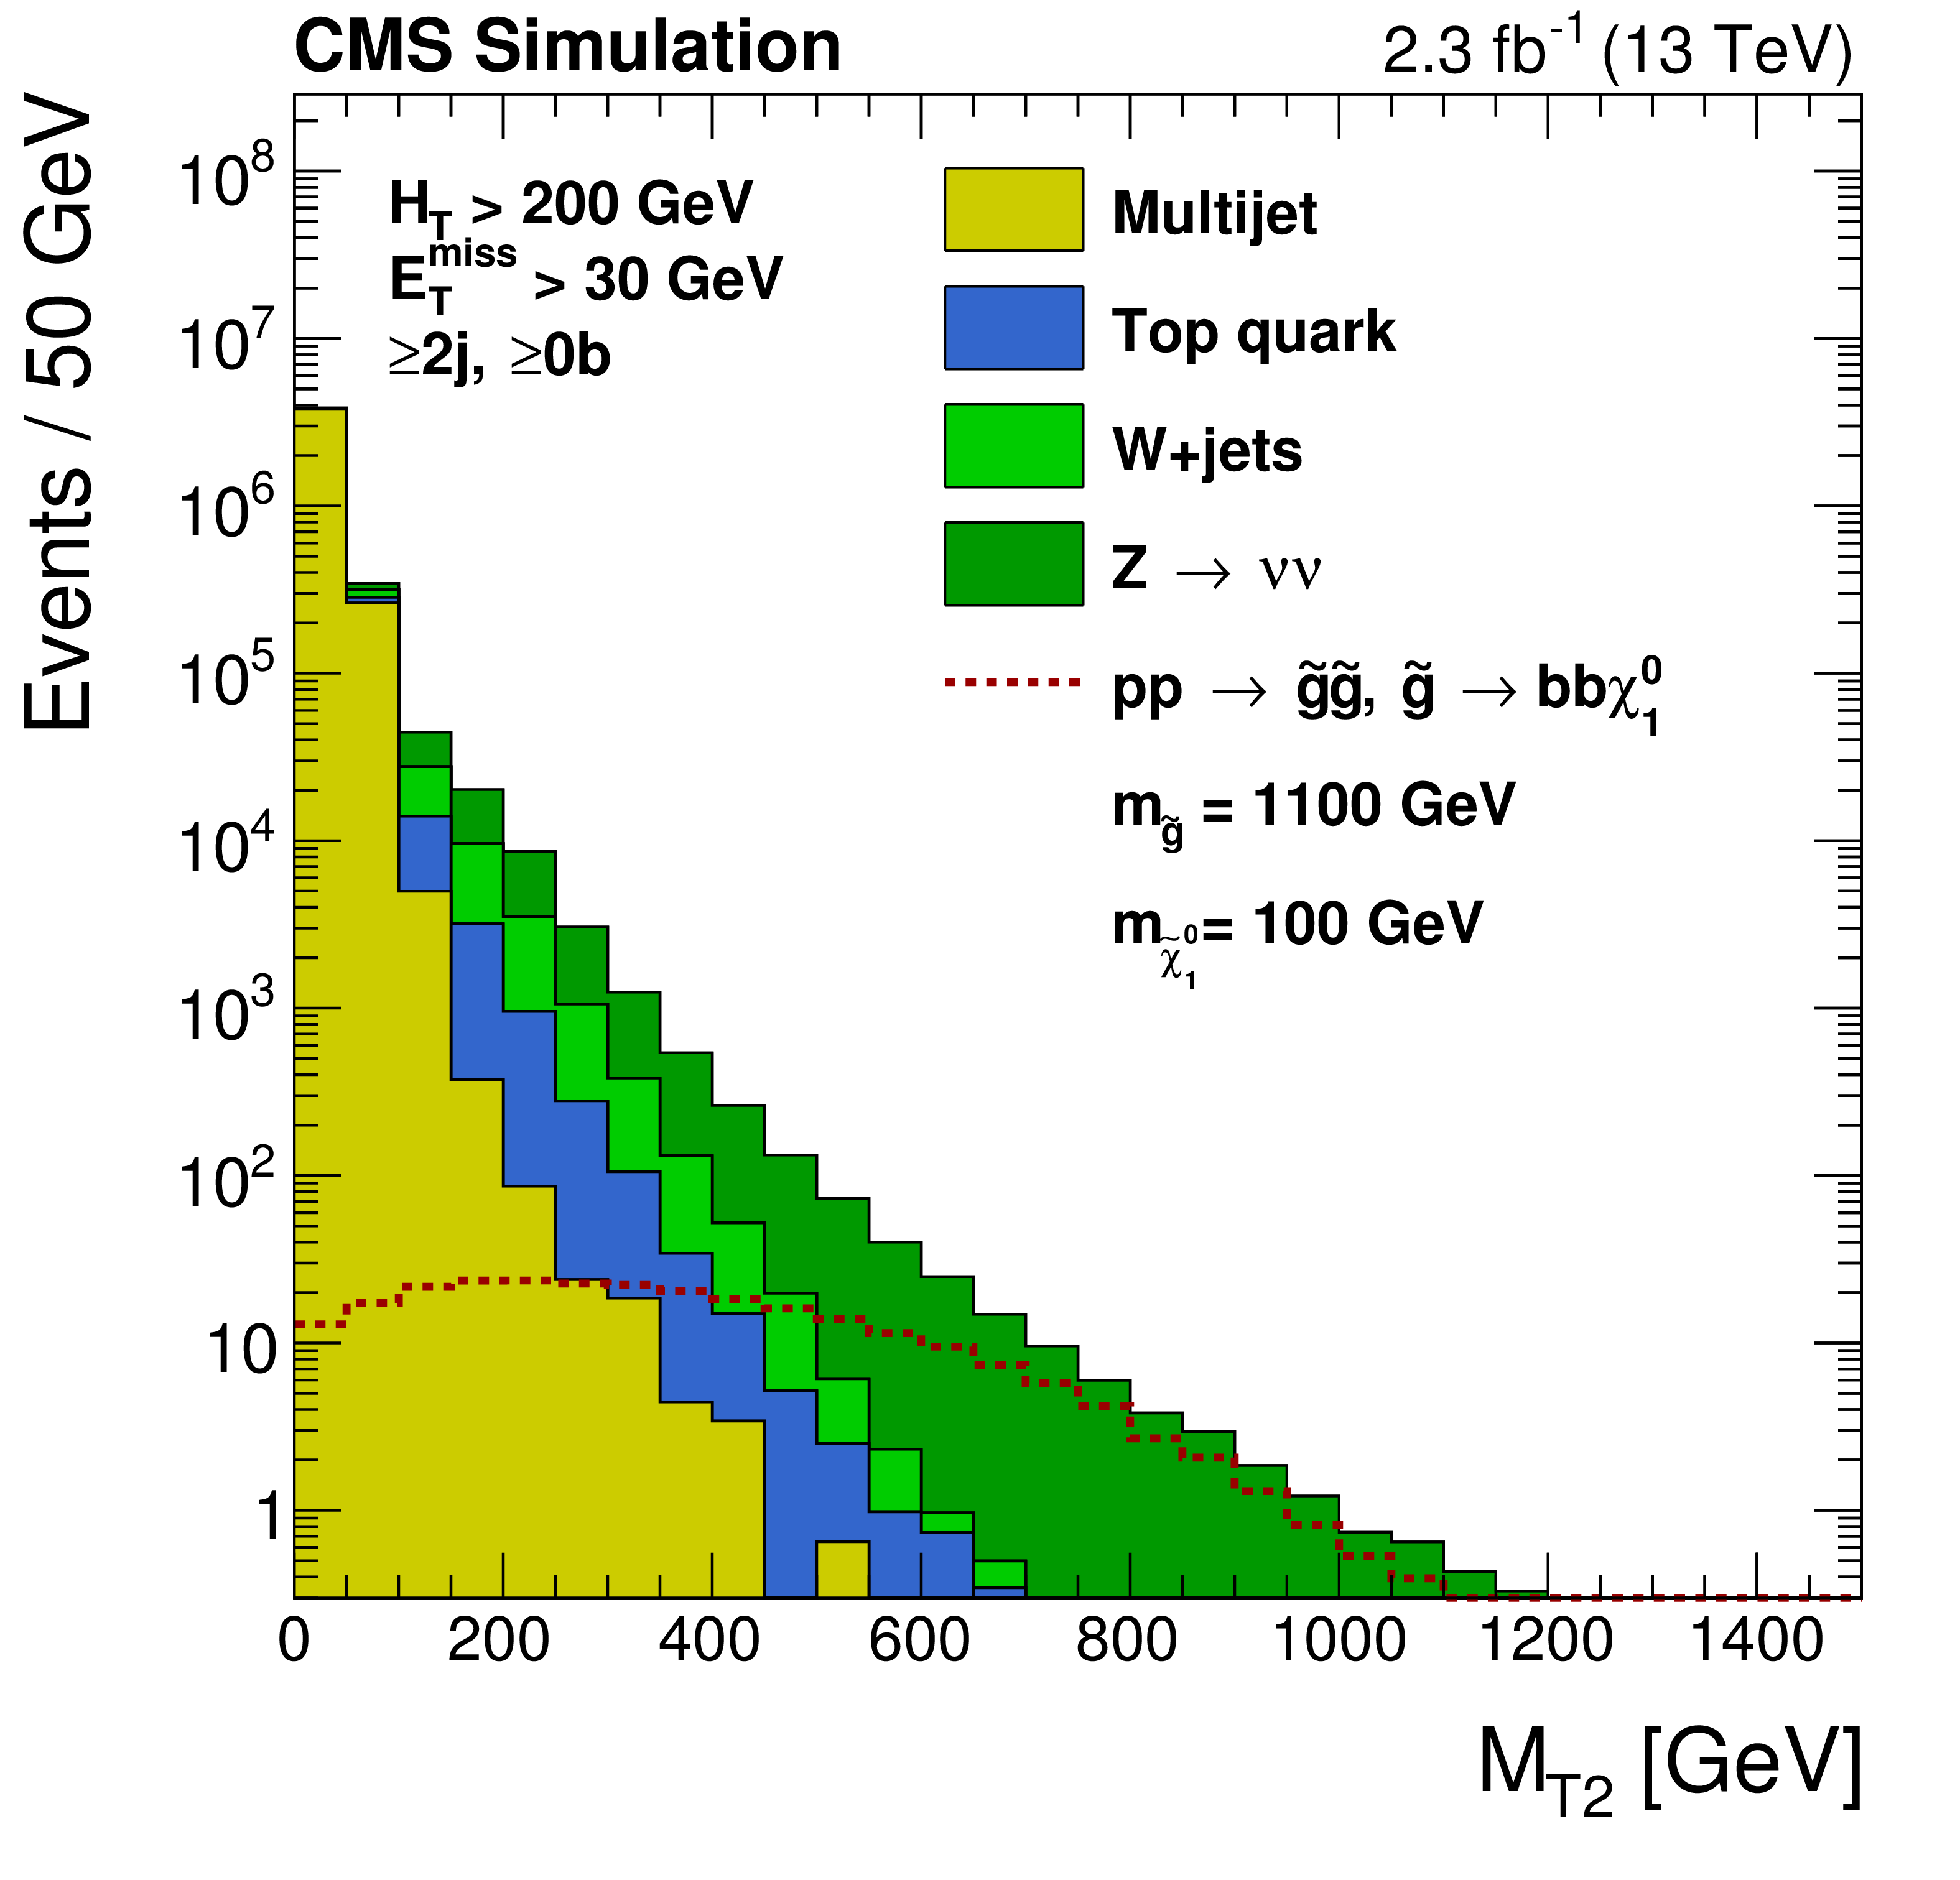
\includegraphics[width=0.48\textwidth]{figures/mt2_mt2_2015.png}
      \caption[\mttwo distributions of backgrounds and an example signal point.]{The distributions in \mttwo of the QCD background (filled yellow) and the neutrino backgrounds (filled blue and green) are stacked and overlaid with an example signal point (gluino pair production and decay to bottom quarks, in red). Even with other mismeasurement-suppression selections applied, the mismeasurement background still dominates without $\mttwo > 200$~GeV. Taken from \cite{MT2_2015}.}
      \label{fig:mt2dist}
    \end{figure}  
    
    \begin{figure}[h!]
      \centering
      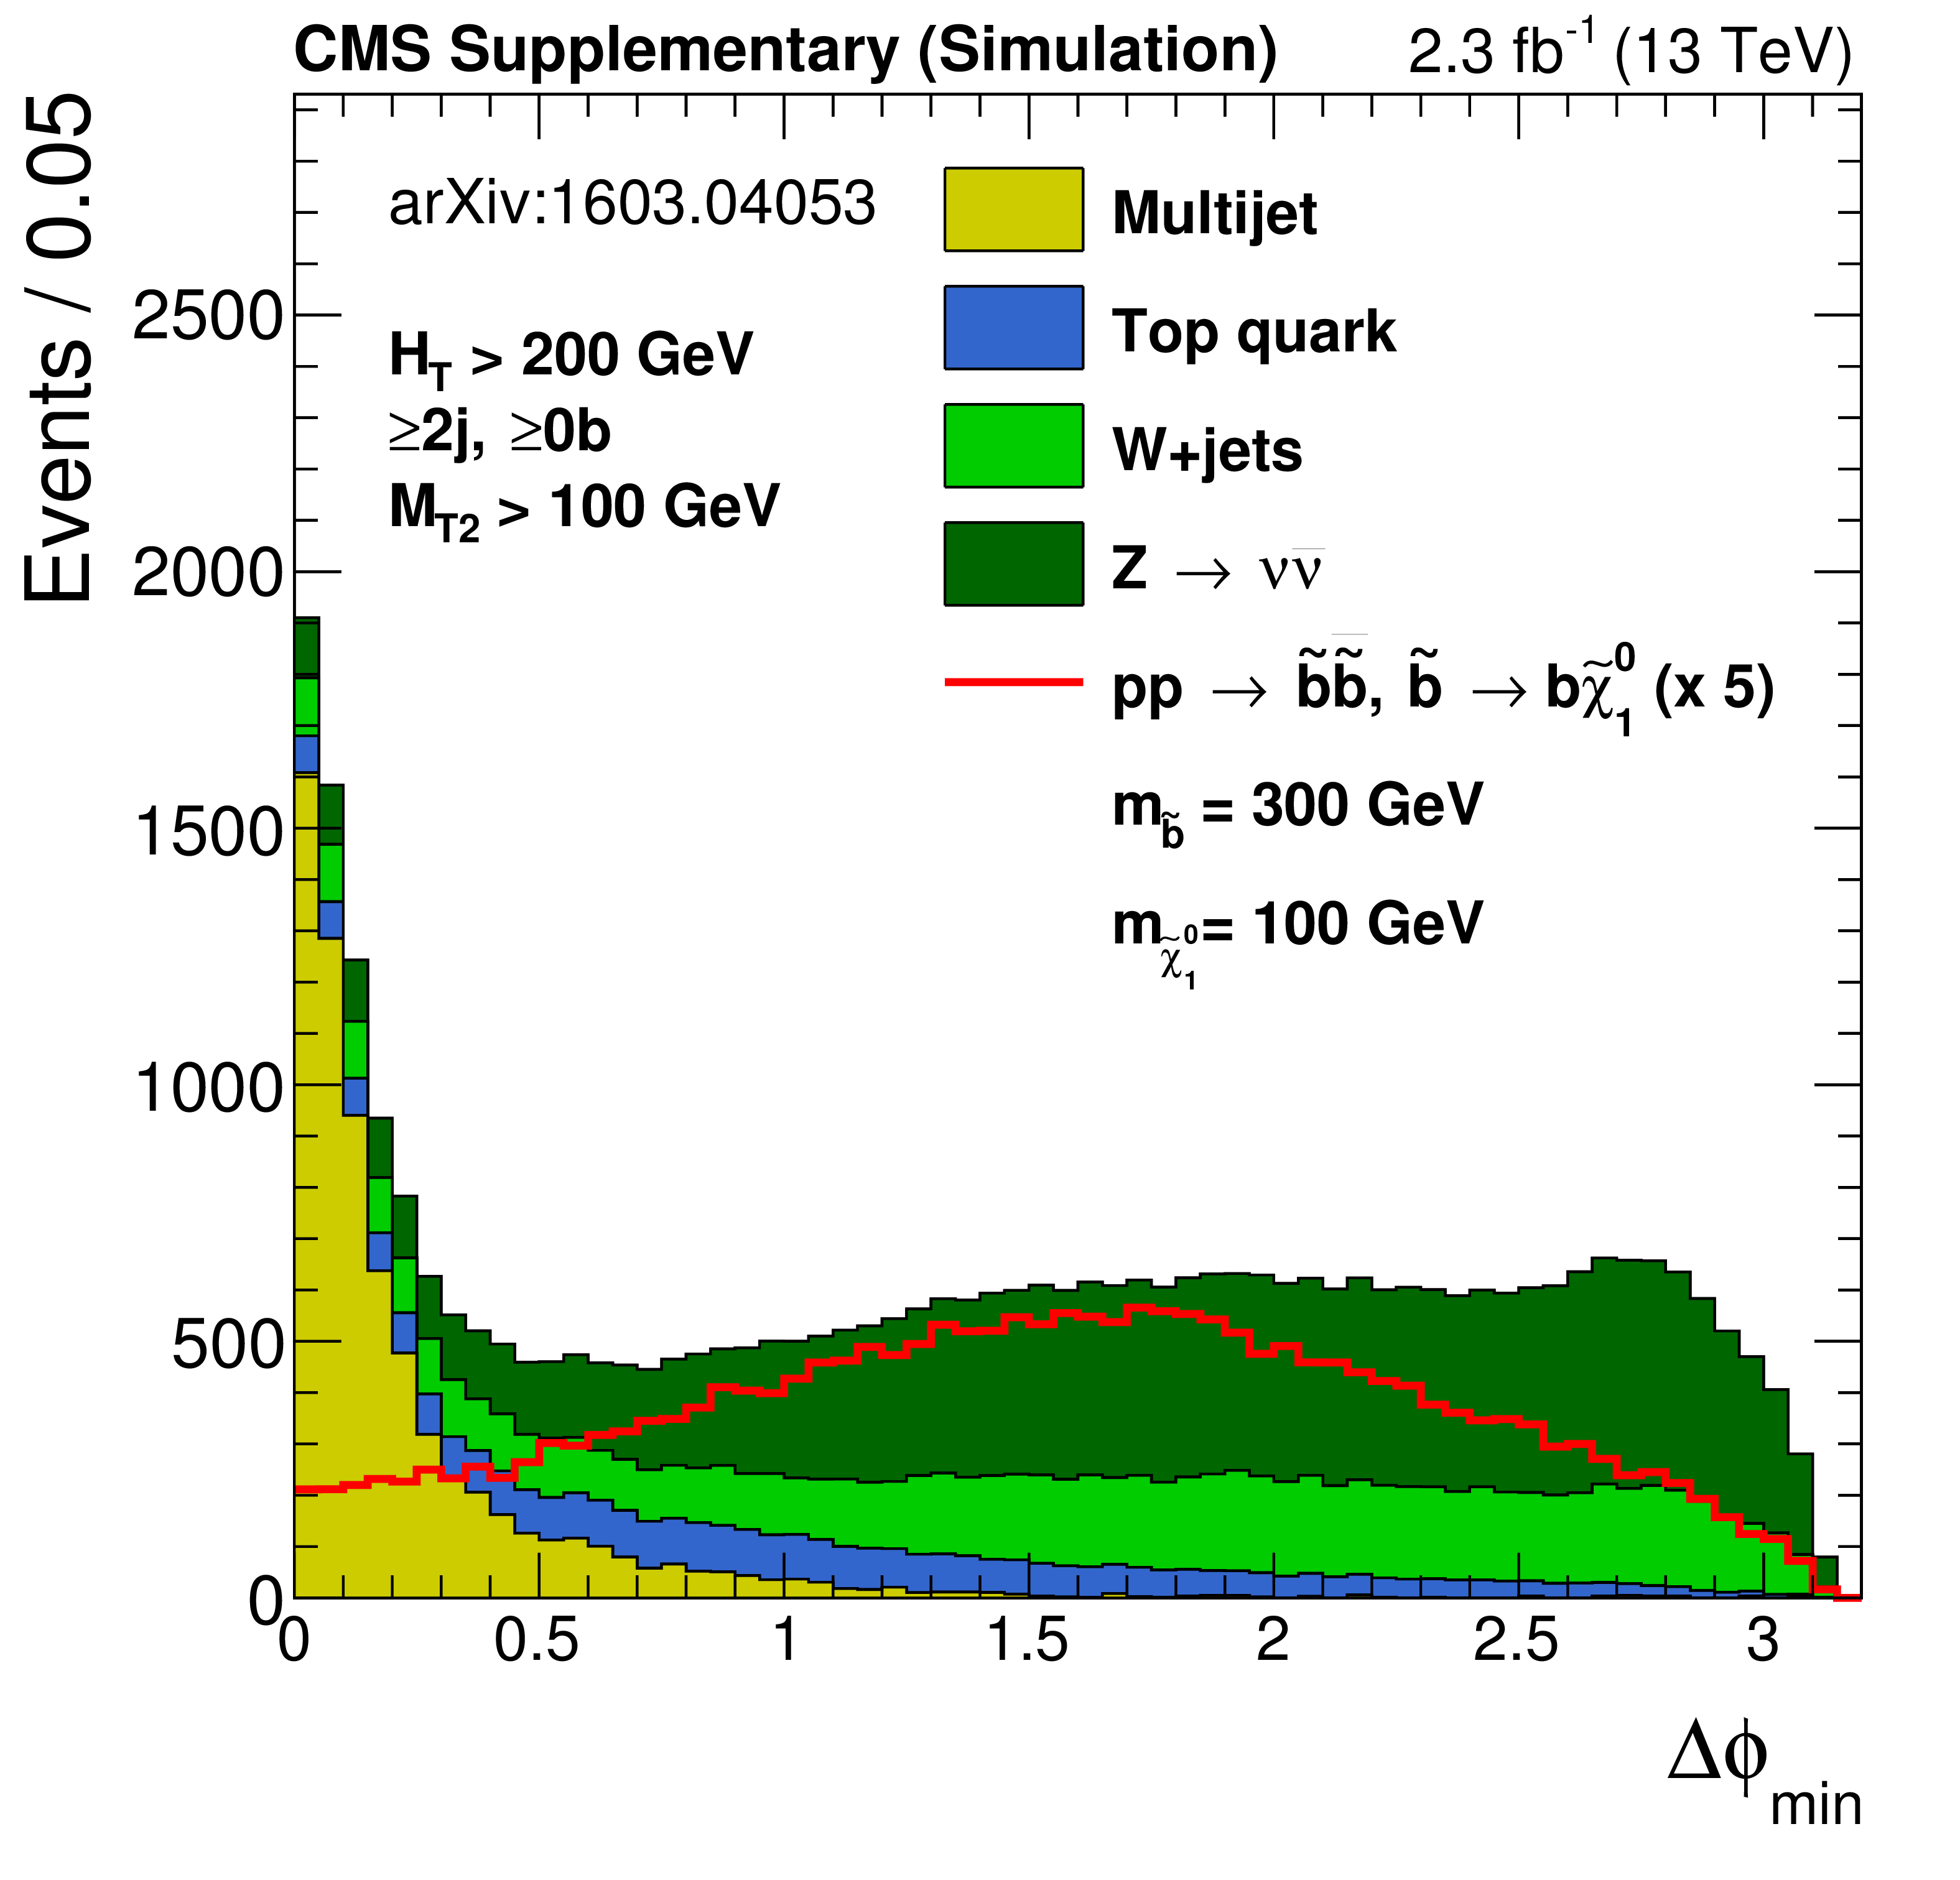
\includegraphics[width=0.48\textwidth]{figures/mt2_dphi_2015.png}
      \caption[\dphimin\, distributions of backgrounds and an example signal point.]{The distributions in \dphimin\, of the QCD background (filled yellow) and the neutrino backgrounds (filled blue and green) are stacked and overlaid with an example signal point scaled up by a factor of 5 (bottom squark pair production, in red), with the \mttwo selection relaxed to 100 GeV. Note that most QCD lies below the cut value of 0.3. Taken from \cite{MT2_2015} supplementary materials.}
      \label{fig:dphimin}
    \end{figure}  
    
    The residual mismeasurement background is estimated using a procedure called Rebalance and Smear that was newly implemented for this edition of the classic analysis, and is described in Section \ref{sec:RandS}.
    
    \subsubsection{Lost Lepton} \label{sec:MT2lostlep}

    The lepton veto rejects most events containing neutrinos originating from the decay of a W boson, $W^{\pm}\rightarrow \ell^{\pm}\nu$.
    However, the lepton is not always successfully reconstructed, usually because it is a $\tau$ that decays hadronically and is mistaken for a meson, and this residual so-called lost lepton background must be estimated. 

    A first attempt might be to simulate events containing W bosons, scale the simulation to the desired luminosity, and count the events in which the lepton is not reconstructed.
    This procedure would have reasonable accuracy, but producing accurate simulations is not trival, and the result would be subject to an array of systematic errors.
    Schematically, if $N_{LL}^{\mathrm{Data}}$ is the actual number of lost lepton events in data and $N_{LL}^{\mathrm{MC}}$ is the number predicted by Monte Carlo simulation, the simulation will mispredict by some factor $\epsilon$ such that $N_{LL}^{\mathrm{Data}} = \epsilon N_{LL}^{\mathrm{MC}}$.

    It is possible to do better than $\epsilon$ with data driven techniques.
    In addition to the lost lepton events, one can also ask the simulation for its prediction of the number of W events in which the lepton is not lost, single lepton events, $N_{SL}^{\mathrm{MC}}$, where the lepton is required to be an electron or muon since $\tau$ reconstruction is much more difficult.
    Every part of this simulation is exactly identical to the lost lepton simulation, subject to almost the same errors, with the major exception being the predicted lepton reconstruction efficiency.
    Call this new error factor $\delta$ so that $N_{SL}^{\mathrm{Data}}=\delta N_{SL}^{\mathrm{MC}}$.
    Then $\epsilon/\delta = \gamma$ is the portion of the misprediction due to the simulation's imperfect knowledge of the lepton reconstruction efficiency and a few other more minor uncorrelated effects, a small portion of the total.
    The ratio $R_{\mathrm{MC}}^{0\ell/1\ell} = N_{LL}^{\mathrm{MC}} / N_{SL}^{\mathrm{MC}}$ is subject only to this relatively small error $\gamma$, since the fully correlated errors cancel.
    The prediction of $N_{LL}^{\mathrm{Data}}$ follows directly,
    \begin{equation}
      N_{LL}^{\mathrm{Data};Est} = R_{\mathrm{MC}}^{0\ell/1\ell} N_{SL}^{\mathrm{Data}}.
    \end{equation}
    The input $N_{SL}^{\mathrm{Data}}$ is measured in a control region populated by single lepton events observed in data, in a kinematic region identical to the corresponding lost lepton signal region.
    The remaining systematic uncertainty is only about 15\% in most signal regions.

    \begin{table}[tbhp]
      \centering
      \topcaption[Table of uncertainties affecting the lost lepton background estimate.]{\label{tab:llepsyst}
        Summary of systematic uncertainties in the lost-lepton background prediction, together with their typical size ranges across the search bins. 
        ($\dagger$) In every topological region, bins along the \mttwo axis with insufficient statistics to allow a fully data-driven estimate are assigned an \mttwo shape from simulation, normalized to the integral of the impacted bins in the data control region.
        Taken from \cite{MT2_2019}.
      }
      \begin{tabular}{ l  c }
        \hline
        Source & Range [\%] \\
        \hline
        Limited size of data control samples & 5--100\\
        Limited size of MC samples & 0--50\\
        $e/\mu$ efficiency & 0--10\\
        $\tau$ efficiency & 0--3\\
        $b$-tagging efficiency & 0--3\\
        Jet energy scale & 0--5\\
        $\Mt\left(\text{lepton},~\vec{\met}\right)$ selection efficiency & 0--3\\
        \mttwo shape uncertainty$^{\dagger}$ & 0--40\\
        Renormalization and factorization scale variation & 0--5\\
        $t\bar{t}b\bar{b}/t\bar{t}jj$ weight & 0--25\\
        \hline
      \end{tabular}
    \end{table}
    Other uncertainties affecting the lost lepton background prediction are summarized in Table~\ref{tab:llepsyst}, together with their typical size ranges across the search bins.
    The first two uncertainties due to limited data control region and Monte Carlo simulation sample sizes are purely statistical.
    The remainder are systematic.

    The efficiency to reconstruct leptons is, as mentioned, the primary uncertainty of the simulation with respect to data, that does not drop out after taking a ratio of lost- and single-lepton events.

    The impact of the $\tau$ reconstruction efficiency is smaller, as it is not used in the single lepton control region, however uncertainty on the rate at which the $\tau$ veto fails to reject events contributes to uncertainty in the expected yield.

    The expected transfer factor from the single lepton to lost lepton regions varies slightly with respect to the binning variables, \Ht, \njet, \nb, and \mttwo, and so is recalculated in simulation for each bin.
    Since the transfer factor varies, they may be incorrectly estimated if simulation does not accurately reproduce the $b$-tagging efficiency and jet energy assignments in real data.

    To restrict the single lepton control region to leptons consistent with originating from a leptonic W decay, the lepton and \met system is required to satisfy $\Mt\left(\text{lepton},~\vec{\met}\right) < 100$~GeV, since an on-shell W can never decay to a lepton-neutrino system more massive than this, and $\Mt \leq M$.

    The renormalization and factorization scales are generic issues with theoretical calculations, discussed in Section~\ref{sec:limitations}.

    Finally, the $t\bar{t}b\bar{b}/t\bar{t}jj$ weight is a special systematic assessed to cover an ad hoc procedure that corrects a particularly severe data-simulation discrepancy affecting the relative rates of $b\bar{b}$ ISR and light flavor ISR in simulated $t\bar{t}$ events.
    This simulation error is not significant for the majority of CMS analyses, however it is important for analyses like this search that include bins with large \nb, for which $t\bar{t}b\bar{b}$ is the only meaningful background.

    In closing, it should be noted that while the lost lepton background tends to be subdominant relative to the Invisible Z background discussed in the next section, it is the largest background in certain high \njet, high \nb, high \Ht bins since Z events do not populate these bins efficiently, while $t\bar{t}$ pair-production events do, and all $t\bar{t}$ events contain two W bosons that may decay leptonically.

    \subsubsection{Invisible Z} \label{sec:MT2zinv}

    The $Z\rightarrow \nu\nu$ background is predicted in a similar fashion to the lost lepton background, using a control region populated with $Z\rightarrow \ell^+\ell^-$ events.
    Again, the leptons are restricted to pairs of electrons and pairs of muons, since $\tau$ reconstruction is much more difficult.    
    Figure~\ref{fig:Zestimate} (right) shows the similarity in the \mttwo distributions of simulated \znunu events and observed \zll events in which one pretends that the leptons are invisible, demonstrating both that these events are kinematically very similar as expected, and that the simulation is accurate.
    The ratio $R_{MC}^{\nu\nu/\ell^+\ell^-}$ can be extracted from Monte Carlo simulation, and is dominated by only the lepton reconstruction efficiency uncertainty.
    In the Standard Model, this ratio is almost exactly 3, but it is significantly larger experimentally because it is possible for one of the leptons in $Z\rightarrow\ell^+\ell^-$ not to be well-reconstructed, causing the affected event not to be counted.
    The value $N_{\ell^+\ell^-}^{\mathrm{Data}}$, unlike $N_{SL}^{\mathrm{Data}}$, is not trivial to extract, since a non-negligible fraction of double lepton events come from sources other than a single Z boson, 
    almost always one each from a pair of W bosons.
    $N_{\ell^+\ell^-}^{MC}$ and $N_{\nu\nu}^{\mathrm{Data}}$ are exclusively $Z\rightarrow \ell^+\ell^-$ and $Z\rightarrow\nu\nu$ events, respectively, and for maximal cancellation of systematic uncertainties, it is desirable that $N_{\ell^+\ell^-}^{\mathrm{Data}}$ be purified to the greatest extent possible.

  \begin{figure}[h!]
    \centering
    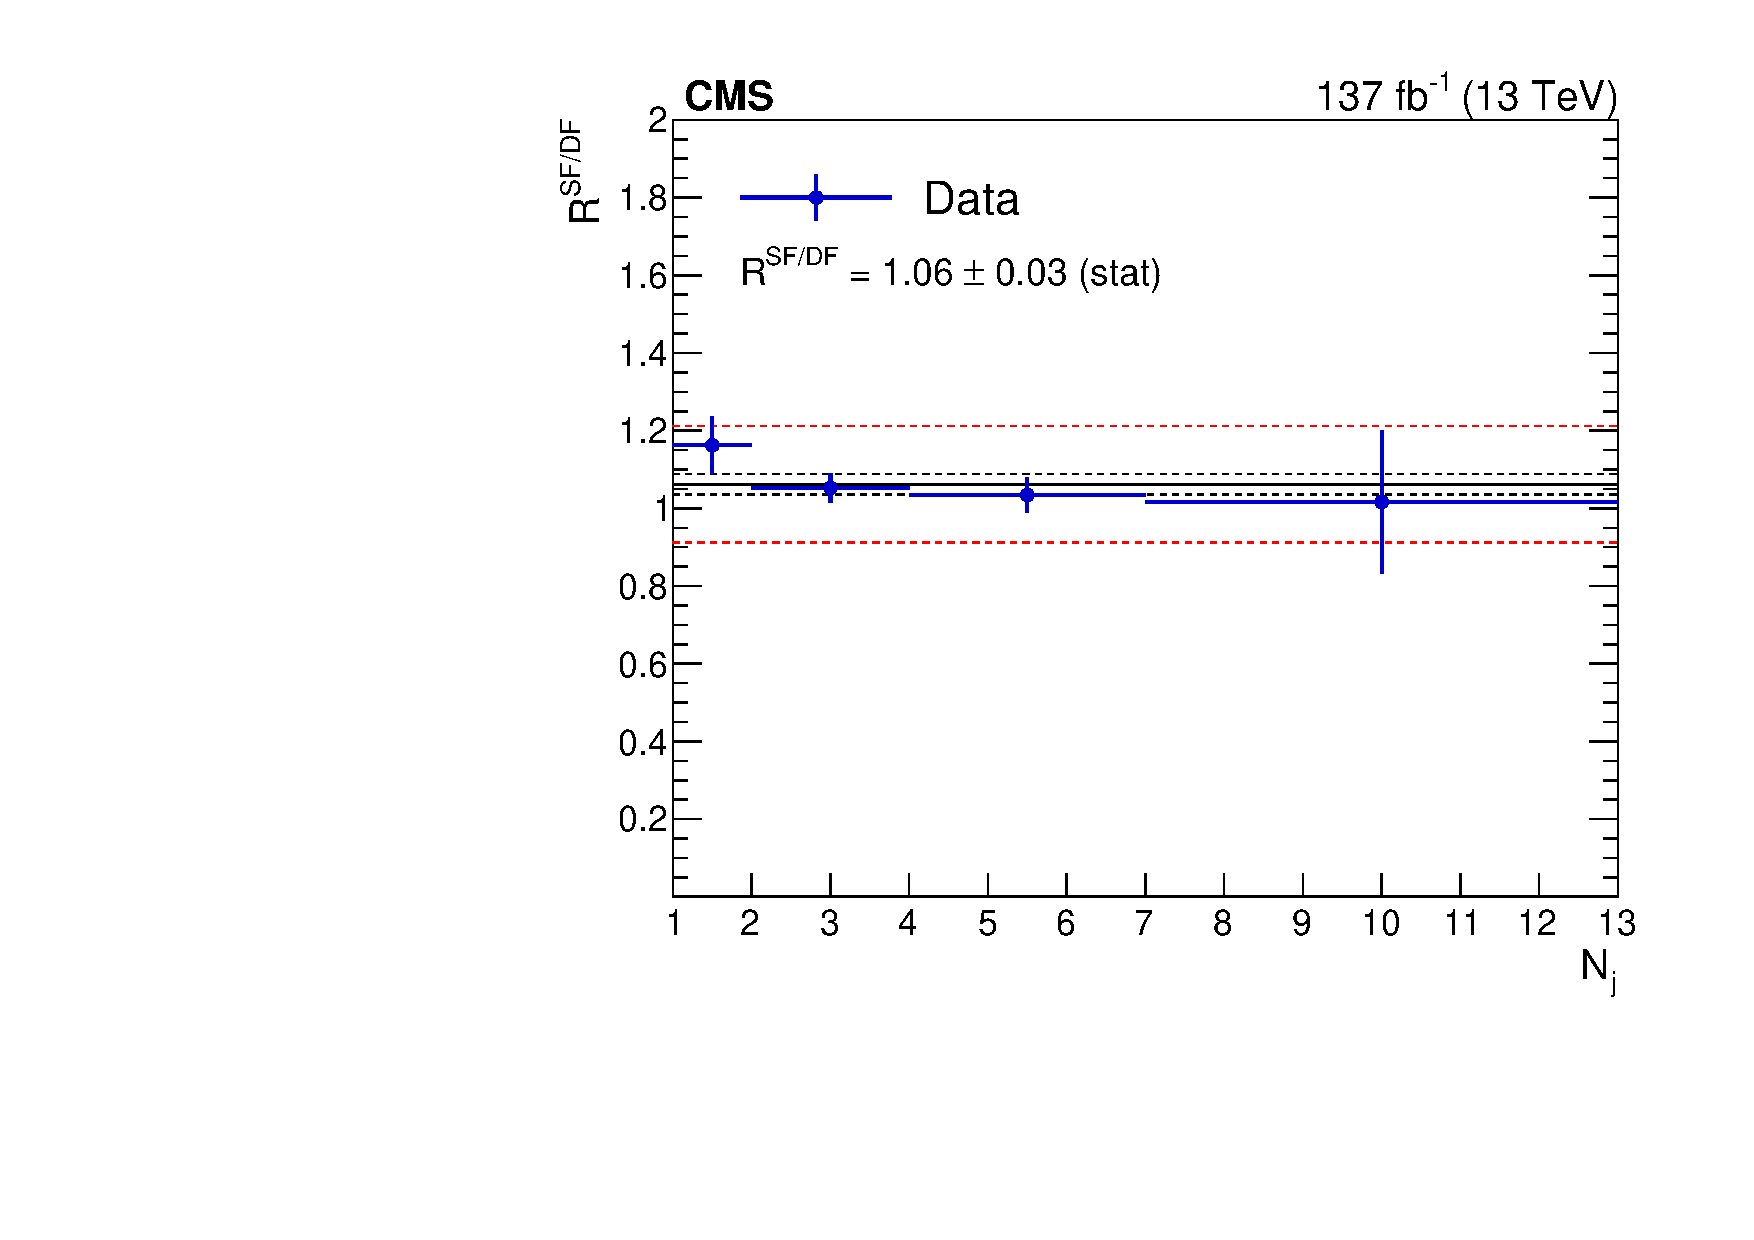
\includegraphics[width=0.53\textwidth]{figures/MT2_2019/Figure_002-a.pdf}
    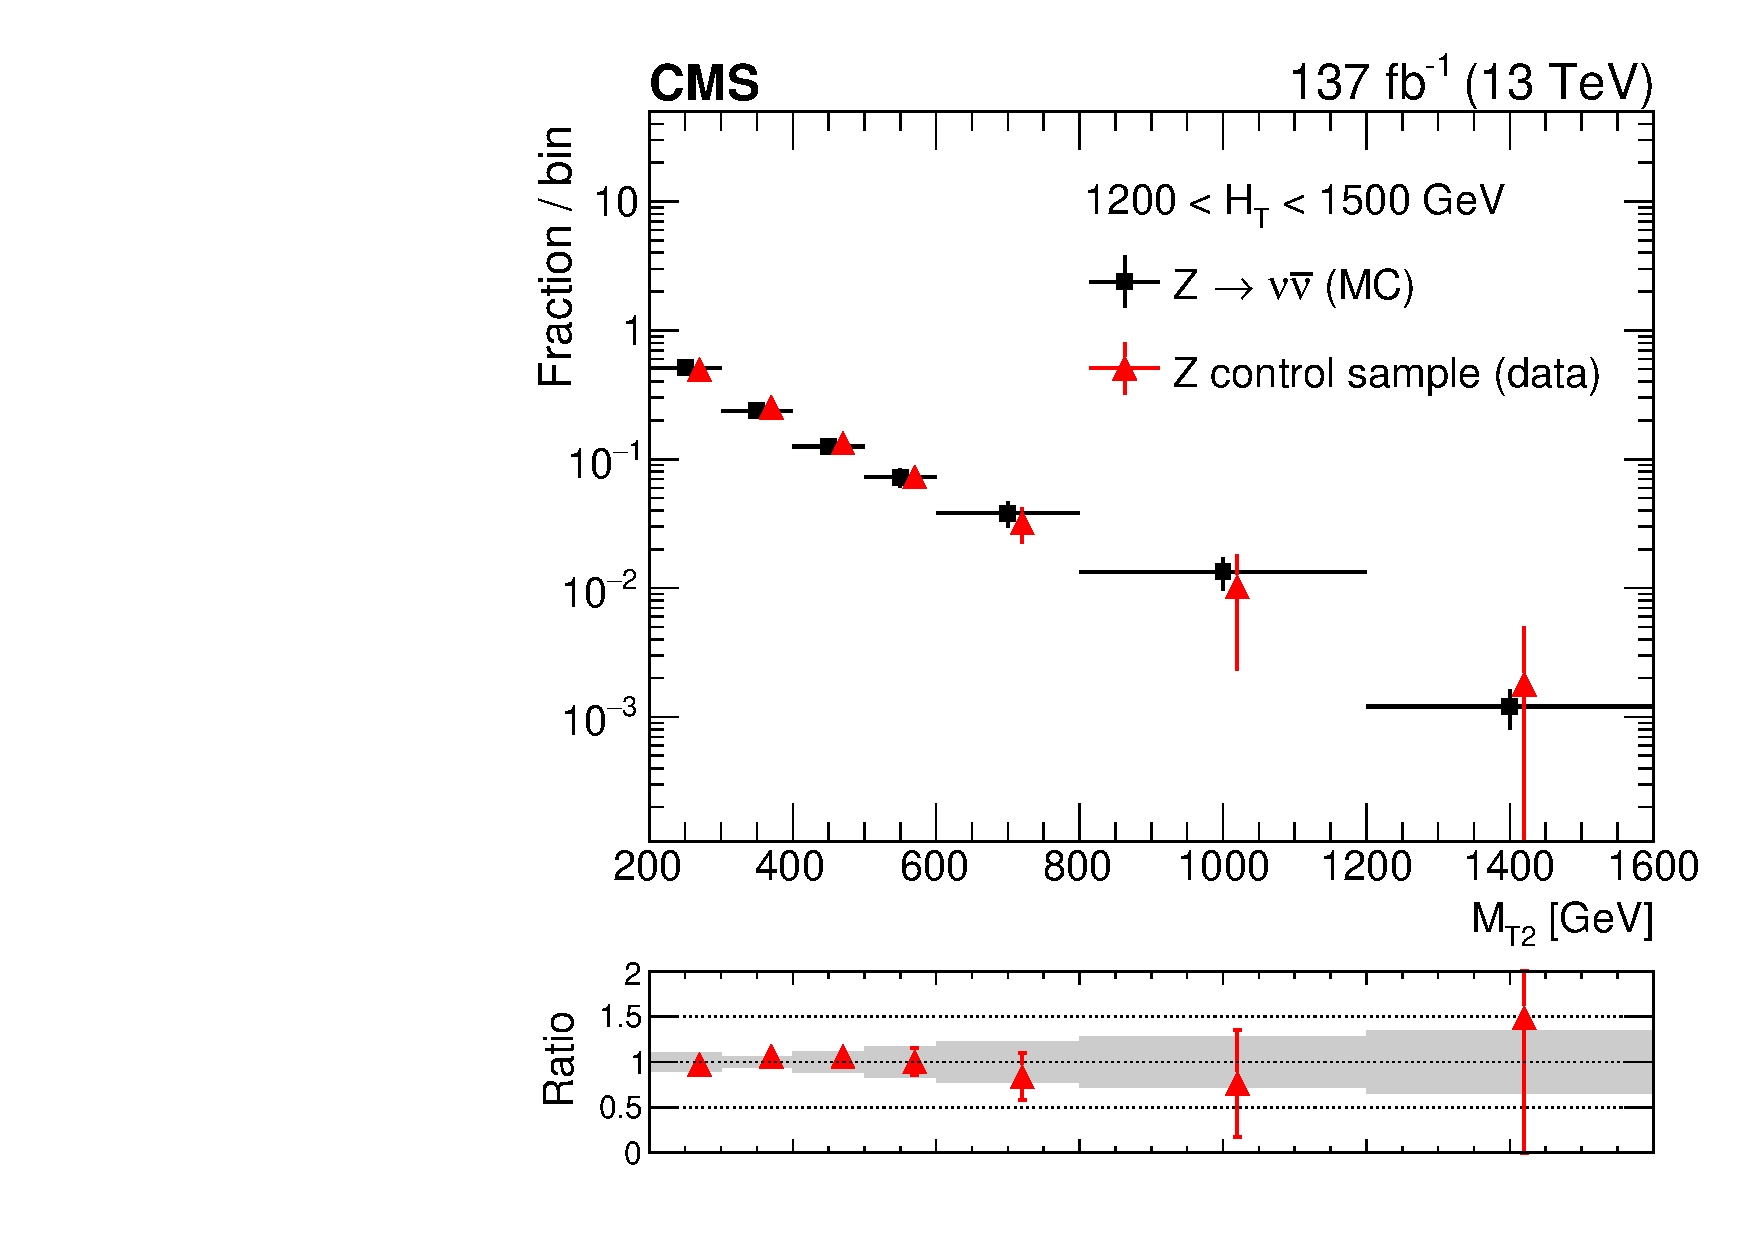
\includegraphics[width=0.44\textwidth]{figures/MT2_2019/Figure_002-b.pdf}
    \caption[(Left) The ratio of the number of same flavor to different flavor lepton pairs in data. (Right) A comparison of the \Mttwo shape between data Z to lepton events and simulated Z to neutrino events.]{
      (Left) The ratio of the number of same flavor to different flavor lepton pairs in data, $R^{SF/DF}$, which is a component of the $Z\rightarrow\nu\nu$ background estimate from $Z\rightarrow\ell^+\ell^-$ events. (Right) A comparison of the \Mttwo shape between data $Z\rightarrow\ell^+\ell^-$ events and simulated $Z\rightarrow\nu\nu$ events. The two processes should be kinematically identical, and the similarity of the distributions indicates that the Monte Carlo simulation models the processes well. Taken from \cite{MT2_2019}.}
    \label{fig:Zestimate}
  \end{figure}  

    Fortunately, there is an experimental handle on the contamination.
    When a Z boson decays to a lepton pair, the flavor is always identical, either two electrons or two muons.
    When a pair of W bosons each decay to a lepton-neutrino pair, their choices of lepton are uncorrelated.
    Half the time, the flavors will be identical as for a Z event, and half the time, one W will decay to a muon and the other to an electron.
    The first case is the undesired impurity in $N_{\ell^+\ell^-}^{\mathrm{Data}}$, and events of the second type are used to populated a different-flavor control region used to predict the impurity, $N_{DF}^{\mathrm{Data}}$.
    It is nearly sufficent simply to subtract $N_{DF}^{\mathrm{Data}}$ from $N_{\ell^+\ell^-}^{\mathrm{Data}}$ since the different flavor and same flavor W events occur at the same rate.
    However, it is possible that the detector is slightly more or less efficient at reconstructing events where both leptons are the same flavor than events in which they are different flavors, so the different flavor count must be scaled slightly to compensate, by a factor $R^{SF/DF}$.
    $R^{SF/DF}$ is measured in data in $\ell^+\ell^-$ events that are kinematically inconsistent with originating from a Z decay, chiefly due to a requirement that the invariant mass of the lepton pair be at least 20~GeV away from the Z mass.
    One finds that $R^{SF/OF} \approx 1.06 \pm 0.15$, as shown in Figure~\ref{fig:Zestimate} (left).
    The final prediction is
    \begin{equation}
      N_{\nu\nu}^{\mathrm{Data};Est} = R_{MC}^{\nu\nu/\ell^+\ell^-}(N^{\mathrm{Data}}_{\ell^+\ell^-}-R^{SF/OF}N_{DF}^{\mathrm{Data}}).
    \end{equation}
    Being irreducible, the \znunu plus jets background is dominant in the vast majority of bins.

    \begin{table}[tbhp]
      \centering
      \topcaption[Table summarizing the systematic uncertainties affecting the \znunu background prediction.]{\label{tab:invzsyst}
        Summary of systematic uncertainties in the \znunu background prediction,
        together with their typical size ranges across the search bins.
        ($\dagger$) In every topological region, bins along the \mttwo axis with insufficient statistics to allow a fully data-driven estimate are assigned an \mttwo shape from simulation, normalized to the integral of the impacted bins in the data control region.
        Take from \cite{MT2_2019}.
      }
      \begin{tabular}{ l  c }
        \hline
        Source & Range [\%] \\
        \hline
        Limited size of data control samples & 5--100\\
        Limited size of MC samples & 0--50\\
        Lepton efficiency & 0--5\\
        Jet energy scale & 0--5\\
        Uncertainty in $R^{\mathrm{SF}/\mathrm{DF}}$ & 0--5\\
        \mttwo shape uncertainty$^{\dagger}$ & 0--40\\
        \hline
      \end{tabular}
    \end{table}
    The uncertainties in the \znunu background prediction are summarized in Table~\ref{tab:invzsyst} together with their typical size ranges across the search bins.
    Only the uncertainty in $R^{\mathrm{SF}/\mathrm{DF}}$ is unique to \znunu, while the others are shared with the lost-lepton estimate.

  \subsection{Baseline Selection} \label{sec:MT2baseline}

  \begin{table}[htbp]
    \scriptsize
    \centering
    \renewcommand{\arraystretch}{1.3}
    \begin{tabular}{c c l}
      Observable               & Selection   & Notes \\
      \hline
      \mttwo                   & $> 200$~GeV & Only for multijet events. Increased to $\mttwo > 400$~GeV for $\Ht > 1500$~GeV to maintain QCD suppression. \\
      $\pt^{\mathrm{Jet 1}}$   & $> 250$~GeV & Only for monojet events. \\
      \Ht                      & $> 250$~GeV & Motivated by available triggers. Background events at lower \Ht are too common for these events to be always recorded. \\
      \met                     & $> 250$~GeV & Relaxed to $\met > 30$~GeV for $\Ht > 1200$~GeV. Motivated by available triggers. \\
      \dphimin                 & $> 0.3$     & Auxiliary mismeasurement suppression. \\
      $\left|\vec{\HTm} - \vec{\met}\right|/\met$ & $< 0.5$ & Auxiliary mismeasurement suppression. \\
      \nlep                    & $= 0$       & The lepton veto; rejects the majority of $W^{\pm}\rightarrow\ell^{\pm}\nu$ background. \\
    \end{tabular}
    \caption[Summary table of baseline event selection.]{A summary of the baseline event selection for the classic \mttwo search.
      Events are required to have large \Ht, no leptons, and significant missing energy unlikely to be the product of detector mismeasurement or a single undetected particle.}
    \label{tab:baseline}
  \end{table}

  The properties of these signals and backgrounds motivate the baseline event selection summarized in Table \ref{tab:baseline}.
  The \mttwo selection primarily suppresses the mismeasurement background, by many orders of magnitude.
  The \dphimin\, and \HTm selections also help to suppress this background further, until it is smaller than the genuine \met backgrounds.
  The \Ht and \met selections are chosen primarily so that all of the selected events pass the online trigger.
  Backgrounds are so common at $\Ht < 250$~GeV, and $\met < 250$~GeV for $\Ht < 1200$~GeV, that the experiment is unable to record all of the events observed, making this part of the parameter space a poor region to search for a rare signal in any case.
  The lepton veto rejects most $W^{\pm}\rightarrow\ell^{\pm}\nu$ events, so that only events in which the lepton is not reconstructed remain in the signal region, as described in Section \ref{sec:MT2lostlep}, and serves to narrow the analysis' focus to the all-hadronic final state as part of CMS's larger research program.

  In addition to this baseline selection, the analysis bins in \mttwo, \Ht, \njet, and \nb to enhance signal sensitivity as described in Section \ref{sec:newbinning}.

  \subsection{Upgrades in 2019} \label{sec:MT2upgrades}

  The classic search has been performed before at 13 TeV, once in 2015 \cite{MT2_2015} using a 2.3~\fbinv dataset, and again in 2016 \cite{MT2_2016} using 35.9~\fbinv.
  The update in 2019 uses the full dataset from 2016, 2017, and 2018, totaling 137~\fbinv.
  As the analysis is dominated by statistical uncertainties in its most sensitive bins, the increased statistical power is the primary improvement in the update.
  
  The update includes two other major upgrades.

  The first improves the estimate of the mismeasurement background using a technique called Rebalance and Smear.

  The second leverages the increased statistics to expand the signal region binning, better targeting signal models with more extreme jet and b-tagged jet multiplicities, and \mttwo.
  

    \subsubsection{Rebalance and Smear} \label{sec:RandS}

    \begin{figure}[h!]
      \centering
      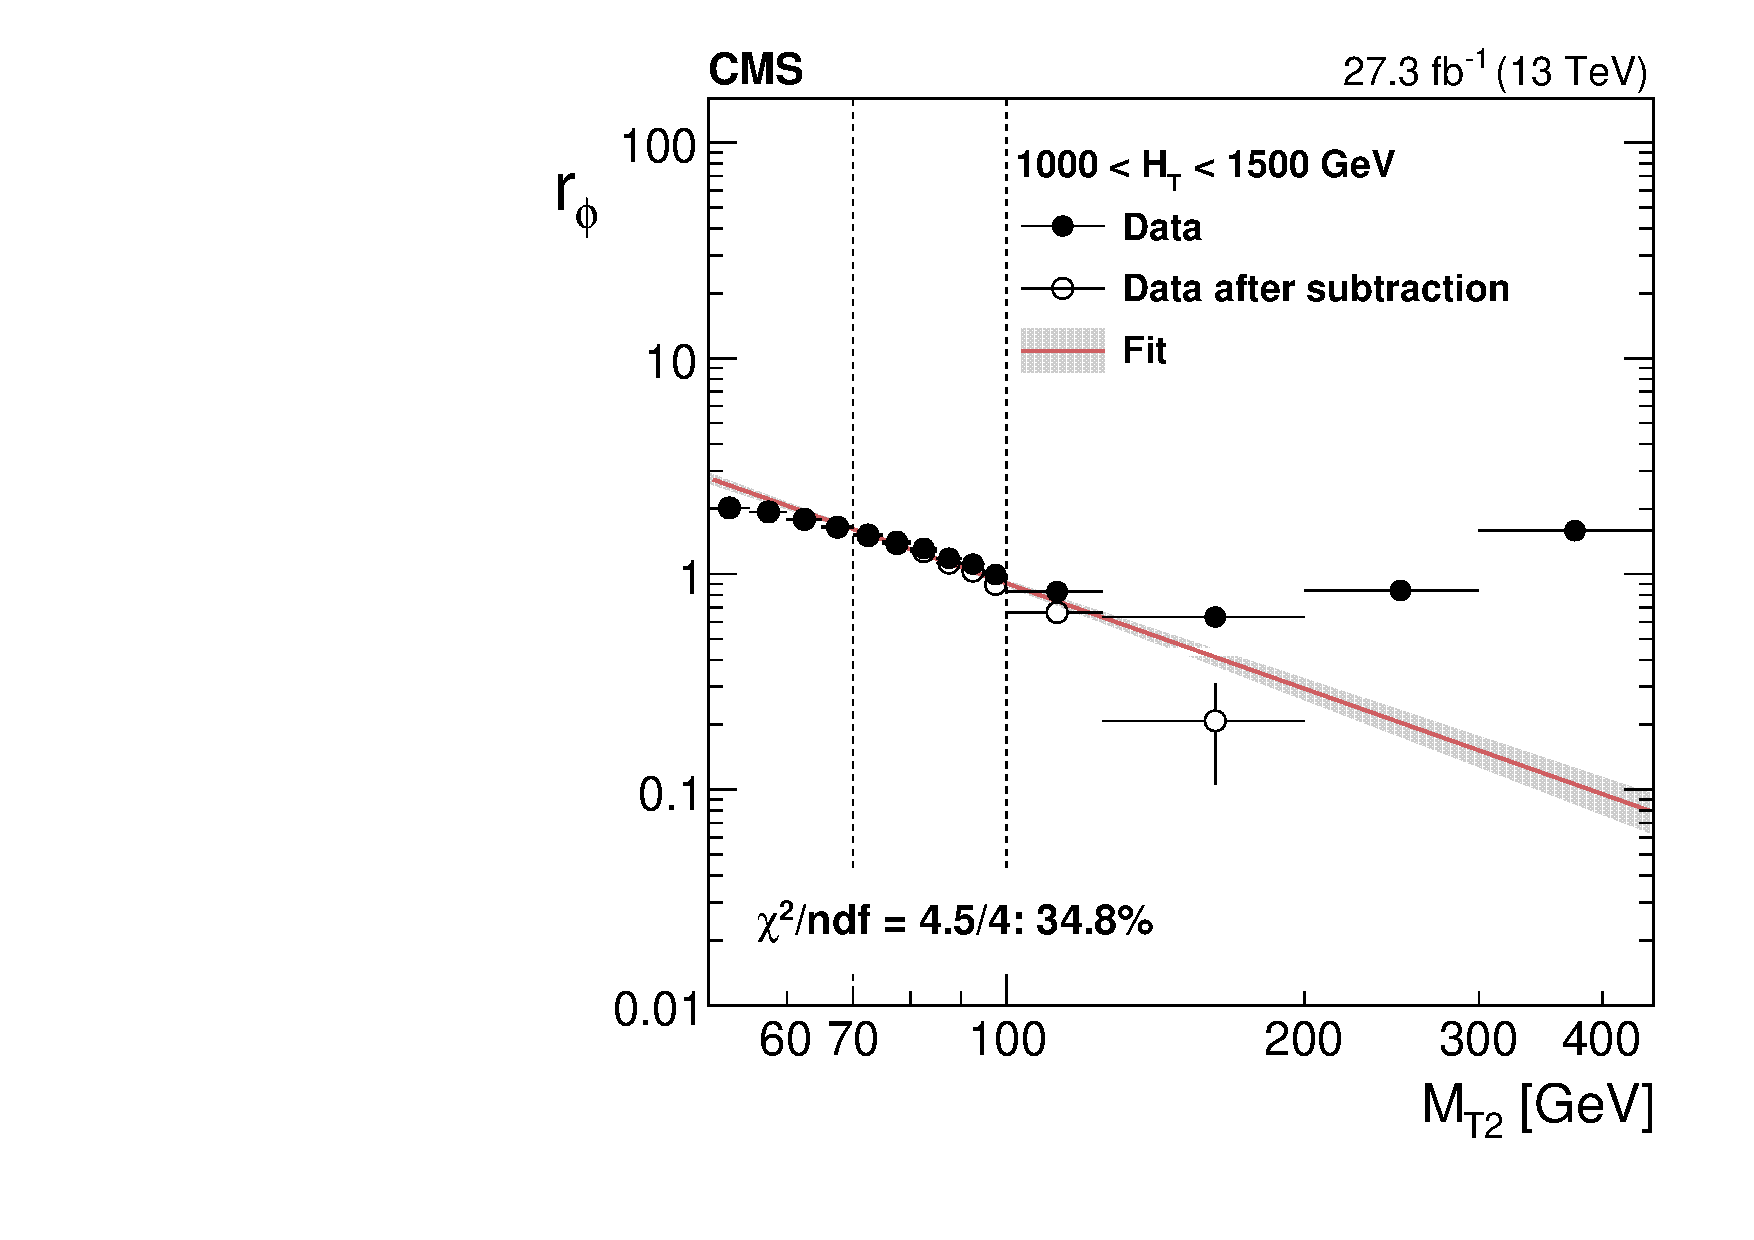
\includegraphics[width=0.85\textwidth]{figures/mt2_rphi_2016.pdf}
      \caption[Fit of $r_{\phi}$ as a function of \mttwo.]{
        The fit of $r_{\phi} = N_{\dphimin > 0.3}/N_{\dphimin < 0.3}$ as a function of \mttwo obtained in the 2016 classic search, for the $1000 < \Ht < 1500$~GeV \Ht band. 
        The fit is performed in events in the \mttwo band $70 < \mttwo < 100$~GeV and extrapolated to the $\mttwo > 200$~GeV signal region.
        Black points represent raw data, while white points represent data after contribution from genuine \met backgrounds is subtracted.
        Taken from \cite{MT2_2016}.}
      \label{fig:rphi}
    \end{figure}  

    In older versions of the classic search \cite{MT2_2015, MT2_2016}, the mismeasurement background estimate used the \dphimin\, observable and extrapolated across \mttwo.
    Events at low \mttwo and at low \dphimin\, are both dominated by QCD mismeasurement.
    The suppression effect of \mttwo is so strong that even events at low \mttwo and {\it high} \dphimin\, are QCD dominated.
    As essentially every low \mttwo event is a QCD event, low \mttwo events can be used to measure the ratio $r_{\phi}$ of QCD mismeasurement events at high and low \dphimin\,.
    High \mttwo events with low \dphimin\, can then serve as a control region for estimating the QCD mismeasurement background, $N_{\dphimin > 0.3} = r_{\phi} N_{\dphimin < 0.3}$.
    Unfortunately, $r_{\phi}$ decreases with increasing \mttwo, so that instead the dependence must be fit to a power law at low \mttwo and extrapolated to high \mttwo, as shown in Figure~\ref{fig:rphi}.
    This procedure has obvious potential for statistical errors in the fit, systematic error in extrapolating the fit to high \mttwo, and potential non-multijet contamination of the low \dphimin\, control region at high \mttwo, producing total relative error at least 40\% and as large as 180\%.
    Although the impact of these errors on the overall analysis is controlled by suppressing the mismeasurement background as described in Section~\ref{sec:MT2QCD}, it is desirable to replace this procedure with a more robust one.

    \begin{figure}[h!]
      \centering
      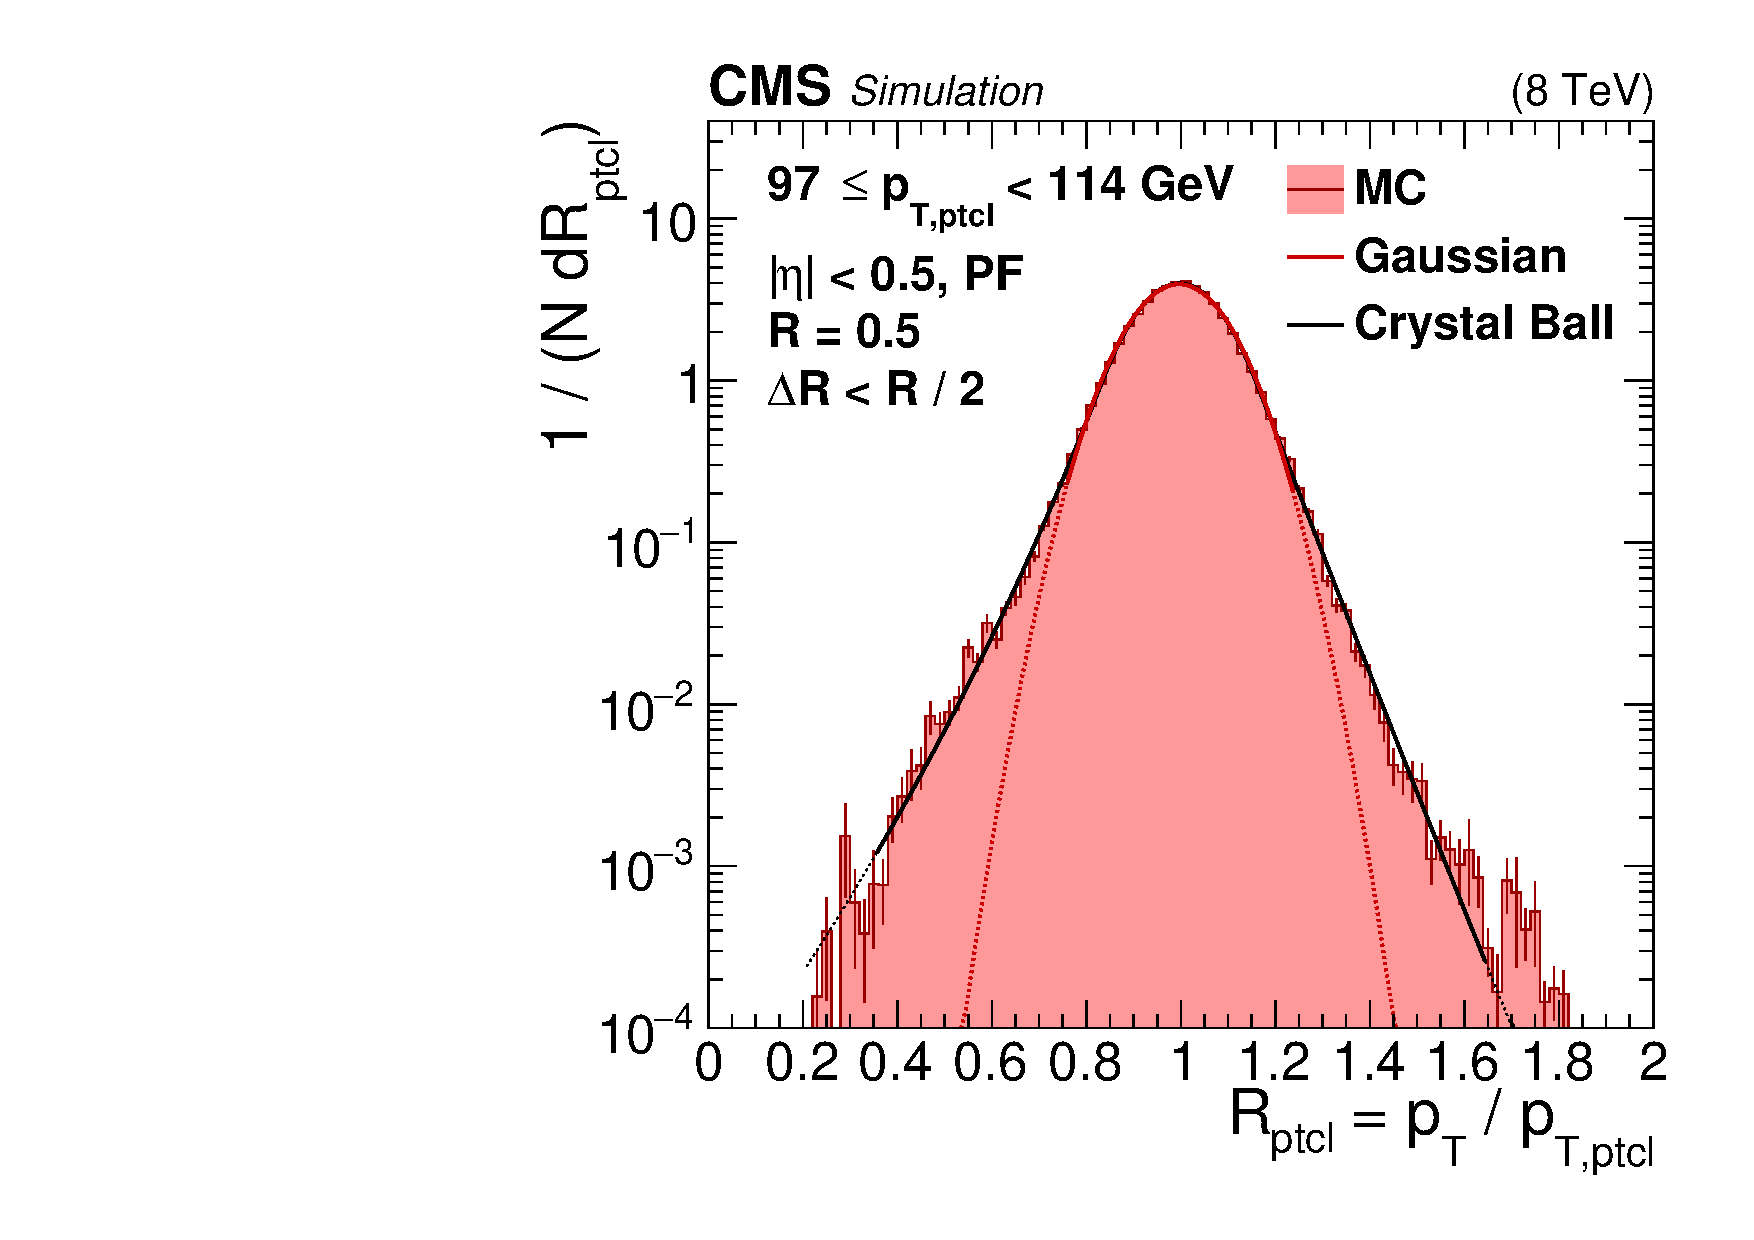
\includegraphics[width=0.85\textwidth]{figures/jet_resolution.pdf}
      \caption[Example plot of jet energy resolution template.]{
        $\mathrm{p}_{\mathrm{T,ptcl}}$ is the ``particle level'' \pt, the total energy that the jet's particle components actually had, while \pt is the energy measured by the detector.
        The horizontal axis is the ratio of these two quantities, and the vertical axis the probability that a jet's measured energy will differ from its true energy by that ratio.
        The response curve shown here applies to jets with particle level \pt in the band $97 < \pt < 114$~GeV, and measured in the CMS barrel.
        Large mismeasurements of jet energy are much less probable than small mismeasurements.
        The core is well-described by a Gaussian, but the tails are highly non-Gaussian and best described by a Crystal-Ball function.
        Taken from \cite{jet_resolution}.}
      \label{fig:jet_resolution}
    \end{figure}  


    Rebalance and Smear (R\&S) achieves the desired improvement.
    R\&S begins with a sample of multijet events from data with \Ht on the order of hundreds of GeV and at least two jets with $\pt > 10$~GeV.
    This is as nearly unbiased a sample of QCD events as is allowed by available triggers.
    These events will generically have some small but nonzero \met due to imperfect measurement of the jet energies, dictated by the detector's resolution, jets from pileup, very low energy objects in the event, and potentially a very small contribution from genuine neutrinos produced in the hadron decay chains inside the jets.
    The \pt values assigned to the jets are then adjusted, finding the most likely assignment of \pt values subject to the hypothesis that the true \met is very nearly zero, and that jet mismeasurements of a given size occur with probability given by jet response templates.
    As shown in Figure~\ref{fig:jet_resolution}, large mismeasurements are rare.
    Thus, the Rebalancing step tries to get the \met as close to zero as feasible without making more improbable adjustments to the jets than necessary.
    The output of the Rebalancing step is a large sample of real QCD events with maximally accurate jet \pt assignments.

    Then, each of these events goes through a Smearing step.
    This step randomly assigns a new \pt to each jet in the event according to the same jet response templates.
    The vast majority of the time, the new event looks as unremarkable as the original event before Rebalancing.
    Rarely, the output event passes the baseline selection and represents a potential mismeasurement event that might lie in the data signal region.
    The Smearing can be repeated as many times for each event as is desired, subject to computing limitations.
    The number of Smeared events falling into each signal region, from this sample of known equivalent integrated luminosity, can then be converted into the expected number of events that would fall into the signal region in data, due to jet mismeasurement.
    
  \begin{figure}[h!]
    \centering
    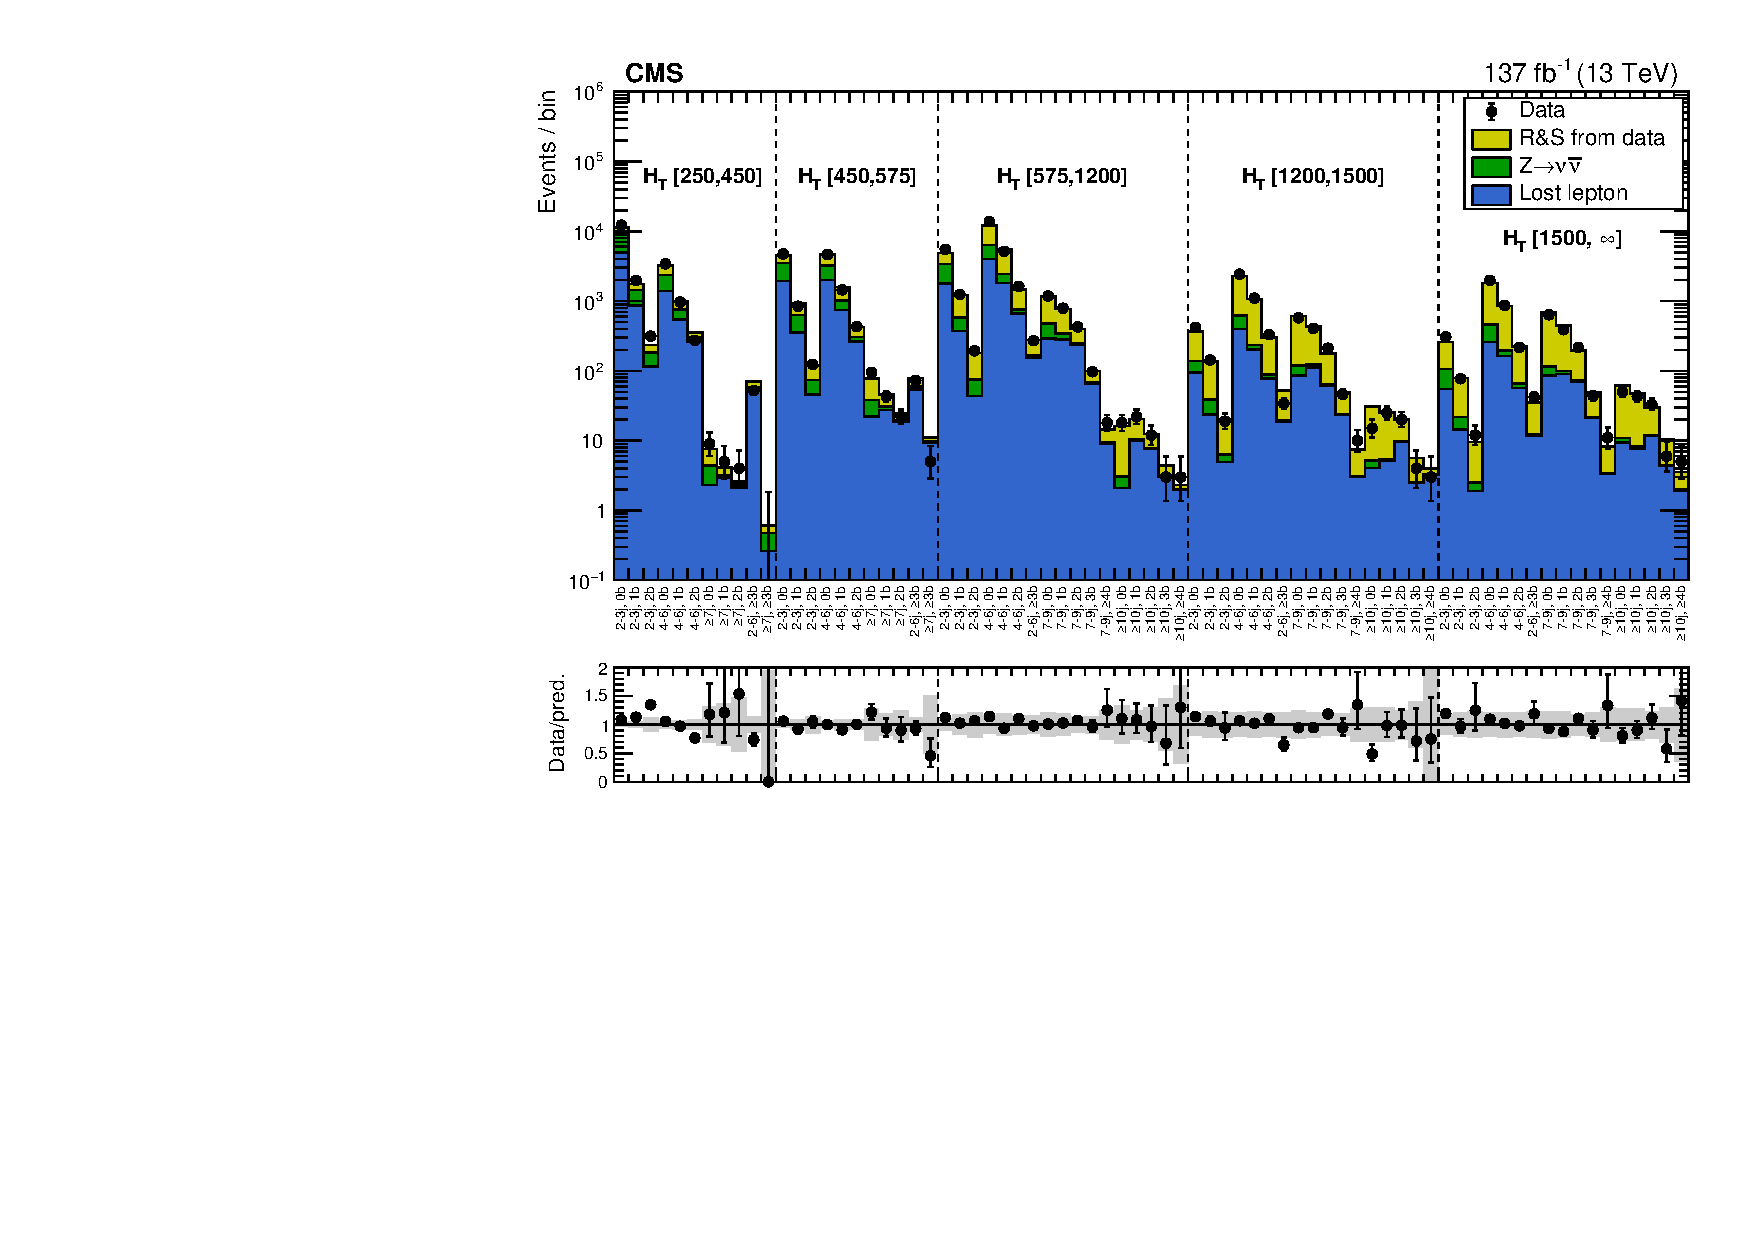
\includegraphics[width=0.85\textwidth]{figures/MT2_2019/Figure_003.pdf}
    \caption[Validation of the Rebalance and Smear jet mismeasurement background estimate in the $\dphimin < 0.3$ control region.]{
      The Rebalance and Smear jet mismeasurement background estimate is validated in the $\dphimin < 0.3$ control region. 
      The multijet mismeasurement event count predicted by Rebalance and Smear is shown in yellow, and contributes most of the event counts in this control region. 
      The combined background estimate (filled histogram) is consistent with the data observation (black data points).
      Taken from \cite{MT2_2019}.}
    \label{fig:RandSval}
  \end{figure}  

    Of course, many of the output events will have $\dphimin < 0.3$, falling outside of the signal region into the QCD-dominated low \dphimin\, control region.
    This allows for a validation in data of the R\&S procedure, shown in Figure~\ref{fig:RandSval}.
    The total background estimate is consistent with data in the $\dphimin < 0.3$ control region across all of the analysis bins, with the R\&S estimated counts contributing most of the predicted events.

    \begin{table}[tbhp]
      \centering
      \topcaption[Systematic uncertainties affecting the Rebalance \& Smear jet mismeasurement background estimate.]
                 {\label{tab:qcdsyst}
                   Summary of systematic uncertainties in the multijet background prediction,
                   together with their typical size ranges across the search bins.
                   ($\dagger$) The parameter $\sigma_\text{T}^{\text{soft}}$ is the width of the assumed underlying irreducible \met distribution for a multijet event, used as an input to the Rebalancing step, and so-called because such \met is dominated by low energy objects.
                   The final output is largely independent of the precise choice for this parameter and the shape of the underlying distribution, but a systematic is assessed to cover any observed variations.
                   Taken from \cite{MT2_2019}.
      }
      \begin{tabular}{ l  c }
        \hline
        Source & Range [\%] \\
        \hline
        Jet energy resolution & 10--20\\
        Tails of jet response in templates & 17--25\\
        $\sigma_\text{T}^{\text{soft}}$ modeling$^{\dagger}$ & 1--25\\
        \njet modeling & 1--19\\
        \nb modeling & 1--16\\
        \hline
      \end{tabular}
    \end{table}

    R\&S achieves a significant improvement over the old $r_{\phi}$ based system, effectively eliminating statistical error, and improving the worst case relative error on the mismeasurement estimate from 180\% to less than 50\%.
    Systematic uncertainties are summarized in Table~\ref{tab:qcdsyst} together with their typical size ranges across the search bins.
    The sources of these uncertainties are described either in the text above, or are shared with the uncertainties affecting the genuine neutrino backgrounds.

    \subsubsection{Expanded Binning} \label{sec:newbinning}

    Although the baseline selection defines the class of events in which a signal of interest may be found, most signals will produce a significant number of events in only a subset of the phase space.
    For instance, a signal producing 4 top quarks in the final state (see Figure~\ref{fig:susyproduction} second row, right) will almost always produce events with $\njet \geq 7$, $\nb > 0$, and $\Ht \sim 1$~TeV.
    If the entire set of selected events is considered together, the entire background is combined, potentially hiding a signal.
    If instead the phase space is divided into many separate regions, the background in each region is smaller, so that the background count is as small as possible in the small subset of regions that any given signal actually populates.
    This sensitivity enhancement motivates very fine binning of the signal region.
    The classic search uses \mttwo, \Ht, \njet, and \nb as binning variables.

    In the 2016 version of the classic search \cite{MT2_2016}, the most extreme \njet\xspace bin was $\njet \geq 7$, and the most extreme \nb bin was $\nb \geq 3$.
    This limitation was imposed by limited statistics.
    The background estimate for each bin is performed separately, and the observed counts are subject to Poisson statistical flucuations.
    Binning too finely causes any potential sensitivity gains from better isolating signal to be lost to greater uncertainty in the expected background.
    The analysis binning was updated for the latest edition of the classic search \cite{MT2_2019}, anticipating the improved statistical power.
    The full set of new bins, along with the predicted background counts and observed event counts in data, is available in Appendix~\ref{app:classicbinning}.

    The new binning extends the old binning in three ways.
    First, new $\njet \geq 10$ bins were added to the $\Ht > 1200$~GeV regions.
    This allows for enhanced sensitivity to signals with extremely high jet multiplicity, such as the 4 top signal previously mentioned.
    Similarly, new $\nb \geq 4$ bins were added to these same regions, targeting the same signal.
    Sensitivity to some mass points of this signal model roughly doubled due to the addition of these bins, which have negligible background but appreciable signal counts.
    Finally, \mttwo binning was generally made narrower and the last bin moved to larger \mttwo values, for all signal regions, until the expected background in the last bin was on the order of 1 event.
    In all, there are 282 classic search bins, enhancing sensitivity to a broad array of potential signal models.

  \subsection{Signal Contamination} \label{sec:MT2sigcontam}

  The data driven estimate procedures for the neutrino backgrounds use control regions defined using leptons.
  Signals capable of producing leptons can contaminate these control regions, increasing the observed control region counts above the actual Standard Model production rate.
  This leads directly to an overprediction of background.
  For instance, consider stop pair production followed by decay to tops, as shown in Figure~\ref{fig:susyproduction} (row 3, right).
  Both tops will decay to a W and a bottom quark.
  If one of the W bosons decays leptonically and the lepton is reconstructed, the event will likely enter the single lepton control region.
  The lost lepton background, described in Section~\ref{sec:MT2lostlep}, will be overpredicted,
  \begin{equation}
    N_{LL}^{\mathrm{Data;Est}} = R_{MC}^{0\ell/1\ell} N_{SL}^{\mathrm{Data}} = R_{MC}^{0\ell/1\ell} \left(N_{SL}^{\mathrm{Data;SM}} + N_{SL}^{\mathrm{Data;Sig}}\right).
  \end{equation}
  The background overprediction is $\Delta N = R_{MC}^{0\ell/1\ell}N_{SL}^{\mathrm{Data;Sig}}$.
  For analysis purposes, the overprediction is modeled in simulation and treated as a reduction of the expected signal counts in every affected bin.
  \begin{equation}
    N_{SR}^{\mathrm{Sig;Adjusted}} = N_{SR}^{\mathrm{Sig;Raw}} - \Delta N
  \end{equation}
  This adjustment has the nice property that all terms are linear in the signal strength, so that it does not need to be recalculated for every signal strength considered when performing statistical analysis of the results.
  The same fraction of the signal is lost at every signal strength.
  
  As a result of this loss of sensitivity due to signal contamination, the classic analysis is less effective, all things equal, when used to search for signals that sometimes produce leptons than the naive expectation based on the leptonic versus hadronic branching ratios.
  This is an inevitable consequence of performing an all-hadronic search.

  \subsection{Results} \label{sec:MT2results}

  \begin{figure}[h!]
    \centering
    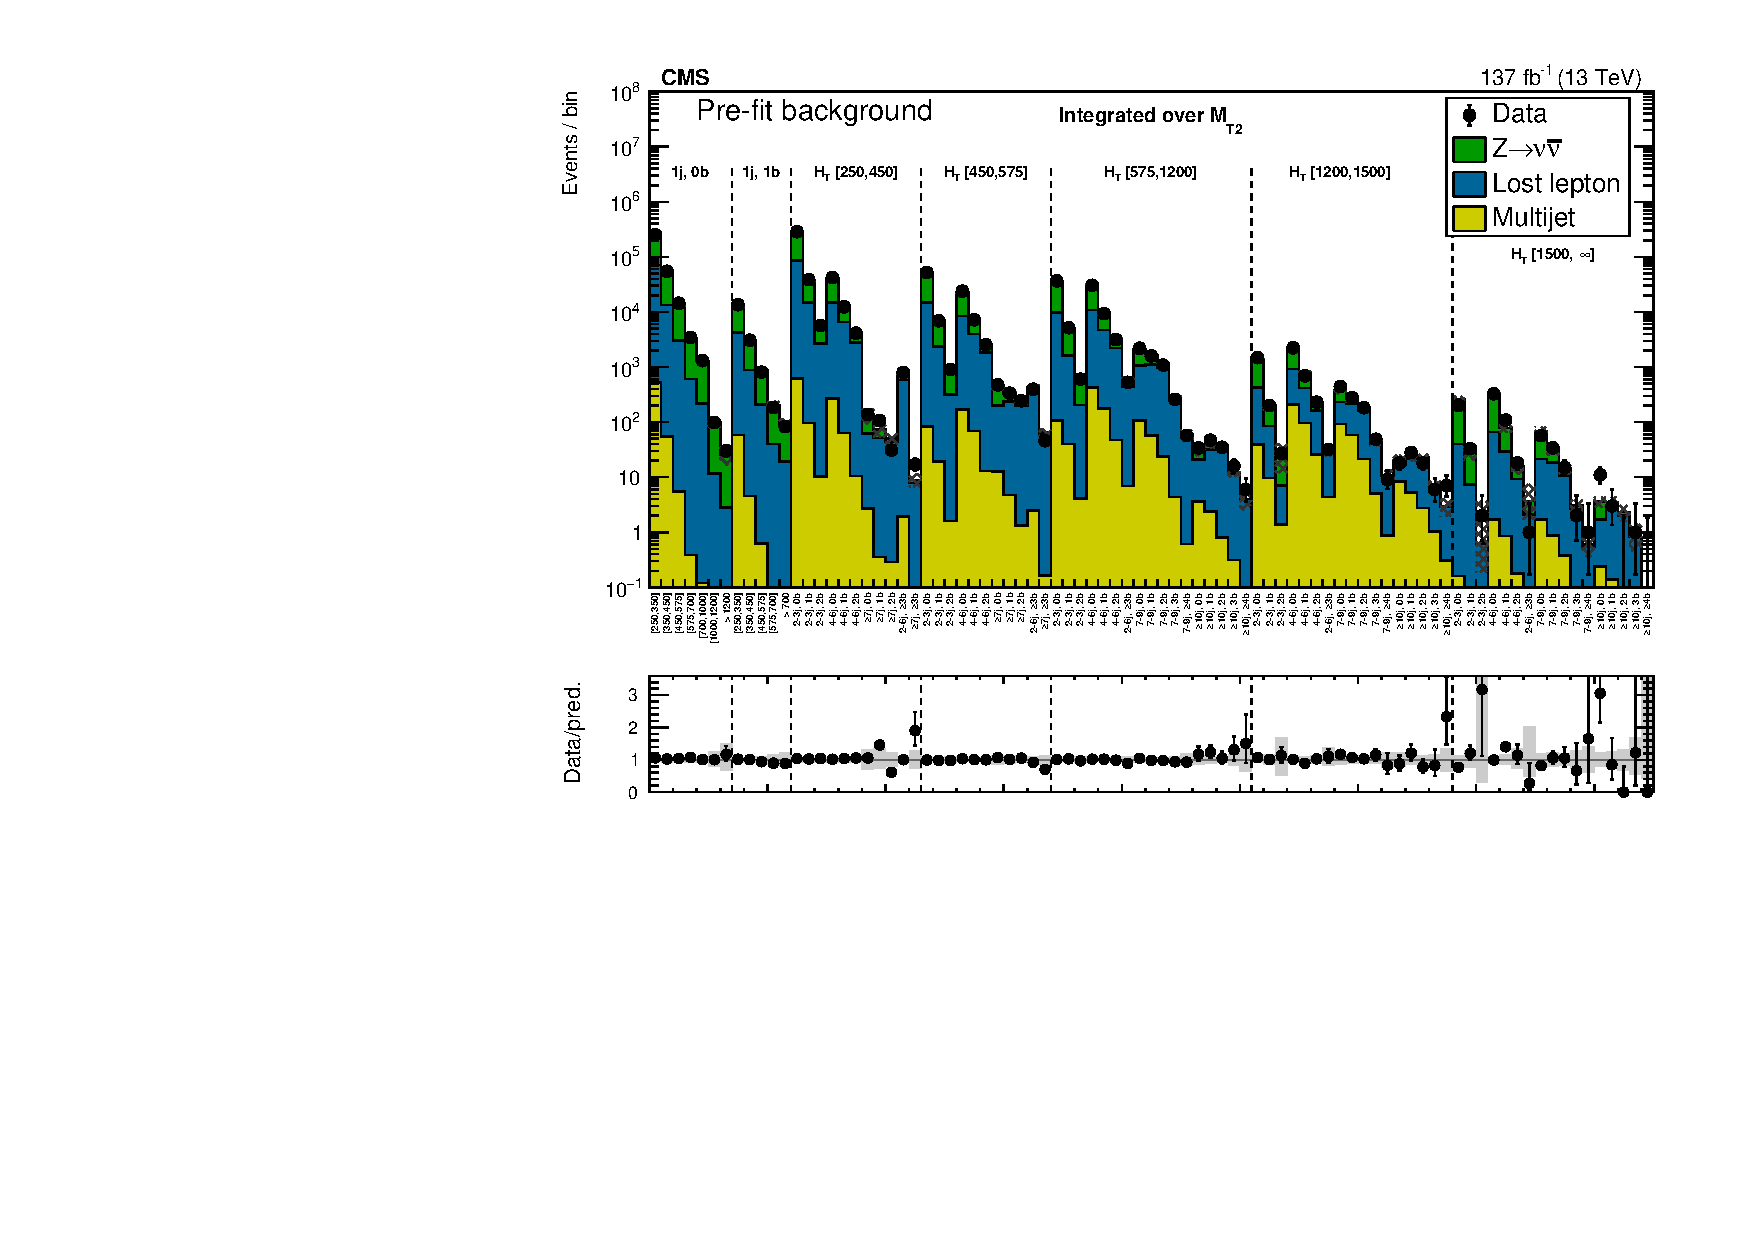
\includegraphics[width=0.85\textwidth]{figures/MT2_2019/Figure_005-a.pdf}
    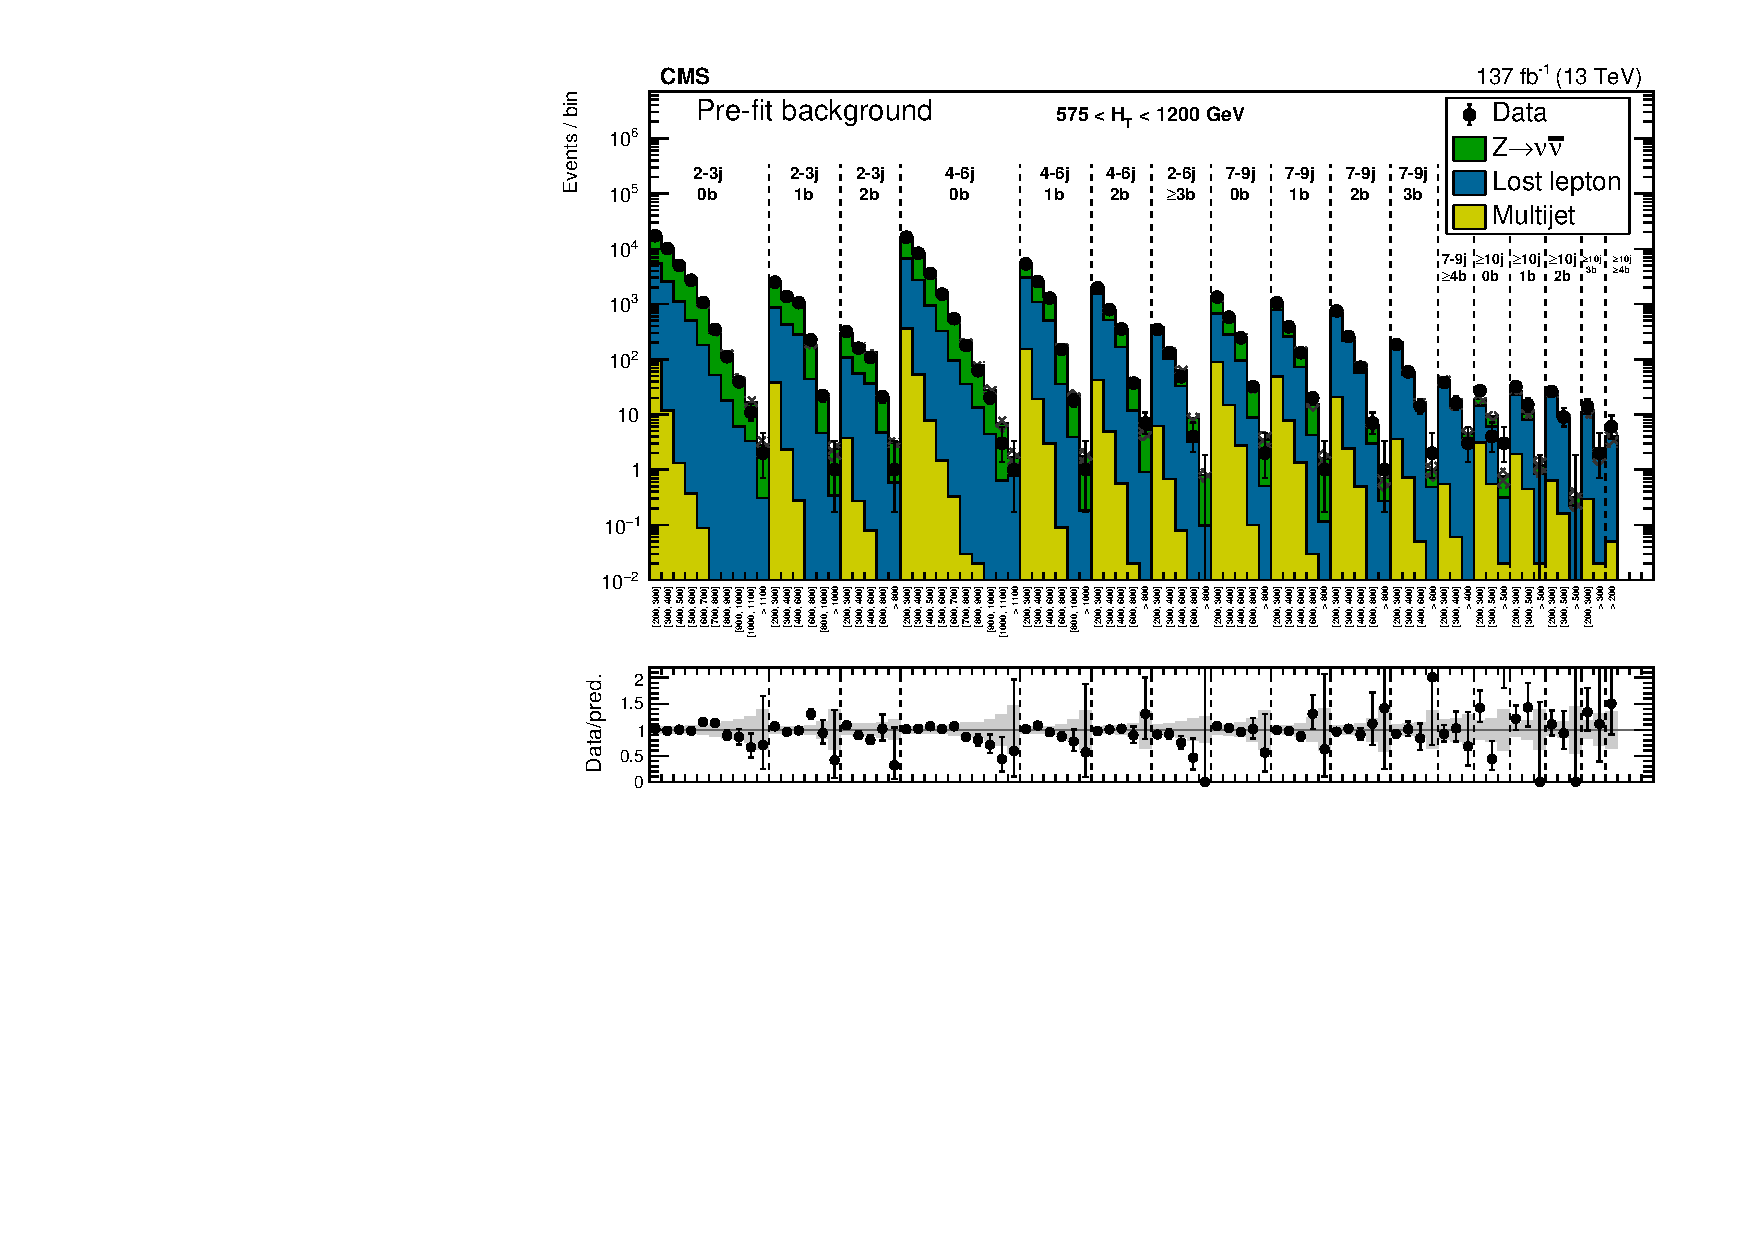
\includegraphics[width=0.85\textwidth]{figures/MT2_2019/Figure_005-b.pdf}
    \caption[Comparison of predicted background and observed data events in the classic search (upper) integrated over \Mttwo and (lower) for each of the medium \Ht search regions.]{Comparison of predicted background and observed data events in the classic search (upper) integrated over \Mttwo and (lower) for each of the medium \Ht search regions. Taken from \cite{MT2_2019}.}
    \label{fig:classicresults}
  \end{figure}  

  The full set of results for every classic search signal region, including every background prediction and the observed count, are available in Appendix~\ref{app:classicbinning}.
  The full set of results integrating over the \mttwo binning are display in Figure~\ref{fig:classicresults} (upper), and the results including the \mttwo binning for the $575 < \Ht < 1200$~GeV bins, the largest set, are shown in Figure~\ref{fig:classicresults} (lower).
  The observed counts are consistent with the background-only hypothesis, and the results are used to set exclusion limits at 95\% confidence level on the signals discussed in Section~\ref{sec:MT2sig}.

  \subsection{Limits} \label{sec:MT2limits}

  The \CL statistical analysis procedure applied in this analysis is decribed in \cite{CLS_method}.
  It begins with maximum likelihood fits to the background-only and signal-plus-background hypotheses, for each signal model, considering each mass point separately. 
  The likelihoods are products of Poisson probabilities for each signal region bin, with log-normal constraint terms for each systematic affecting the predicted counts.
  Correlation between uncertainties affecting different bins are fully accounted for.
  As stated in the previous section, the background-only hypothesis is consistent with the observation.
  So, the parameter of interest for each signal model is the maximum signal cross section that can be excluded with 95\% confidence level.
  That is, the maximum possible production rate that the signal model could have, without requiring a combination of background and signal fluctuations more improbable than 1 in 20 to be consistent with the data.
  If the production cross section excluded at 95\% CL is less than the theoretical cross section for a given signal model, that signal model is said to be excluded at 95\% CL.

  The simplified supersymmetric extensions to the Standard Model shown in Figure~\ref{fig:susyproduction} have only two free parameters, the mass of the pair-produced superpartner, and the mass of the lightest supersymmetric particle, the dark matter candidate \lsp.
  Plotting the gluino or squark mass on the horizontal axis and the mass of \lsp on the vertical axis, then marking the mass points excluded at exactly 95\% CL, produces the exclusion curves shown in Figures~\ref{fig:t5x}--\ref{fig:stop_other}.
  Points to the lower left of these curves are excluded, while points above and to the right are not, as they require fluctuations no more improbable than 1 in 20 to be consistent with present data.

  The CMS dataset was collected only once, and this dataset is subject to fluctuations.
  The multiple exclusion curves shown on each plot, some in red and some in black, provide an indication of how unusual the limits generated by this dataset were.
  Suppose that the background's expected event count in a given region, summing across this entire dataset, is $B$.
  It is clearly possible that the actual number of background events that occur in the dataset in this bin could be around $B+\sqrt{B}$, or $B-\sqrt{B}$.
  In the first case, the analysis will draw unexpectedly weak limits on signals that populate this bin, as the additional background appears consistent with signal.
  In the second case, the analysis will draw unexpectedly strong limits on signals that populate this bin, as there are not even enough events to cover the expected background count.

  The curves shown in red are the median, 1 standard deviation, and 2 standard deviation expected exclusion curves, in the background-only hypothesis.
  Together, these indicate the typical range of exclusion curves across many imaginary CMS datasets in which there is no signal to find.
  The curves in black are those that were observed in the CMS dataset as actually recorded.
  When the black observed curves extend out beyond the red expected curves, the analysis likely benefitted from a downward fluctuation of background.
  In cases where the observed curves swing inward compared to the expected curves, the analysis may have experienced an analogous unlucky upward fluctuation of background that mimicked a small signal, or alternatively there may be a genuine small signal lurking in the data that is resisting exclusion!

  The general shape of the curves is set by a combination of the falling cross section with increasing gluino or squark mass shown in Figure~\ref{fig:SUSYxsec}, and a loss of signal efficiency and signal versus background discriminatory power when the mass splitting between the gluino or squark and \lsp is small.
  On the lower right hand side of the plots lie signals that produce spectacular, energetic events, but at a very low rate due to the large mass of the gluino and squark, and accordingly small pair-production cross section.
  Moving up along the \lsp mass axis towards the upper right, the events remain spectacular, so the exclusion curves remain roughly vertical, limited only by the production cross section.
  Eventually, the mass splitting becomes small enough that the loss of signal efficiency and signal versus background discriminatory power becomes significant, and the exclusion curve turns to the left, towards lower mass squarks or gluinos and higher production rates.
  Decreasing the gluino or squark mass at fixed \lsp mass reduces the mass splitting, so the curve generally must also drop down somewhat along the \lsp mass axis to maintain a reasonable splitting.
  Eventually, the curve intercepts the $M_{\lsp} = M_{\tilde{g}}$ or $M_{\lsp} = M_{\tilde{q}}$ line.
  At this mass and below, all points are excluded even in the limit of zero mass splitting.


\begin{figure*}[htbp]
  \centering
    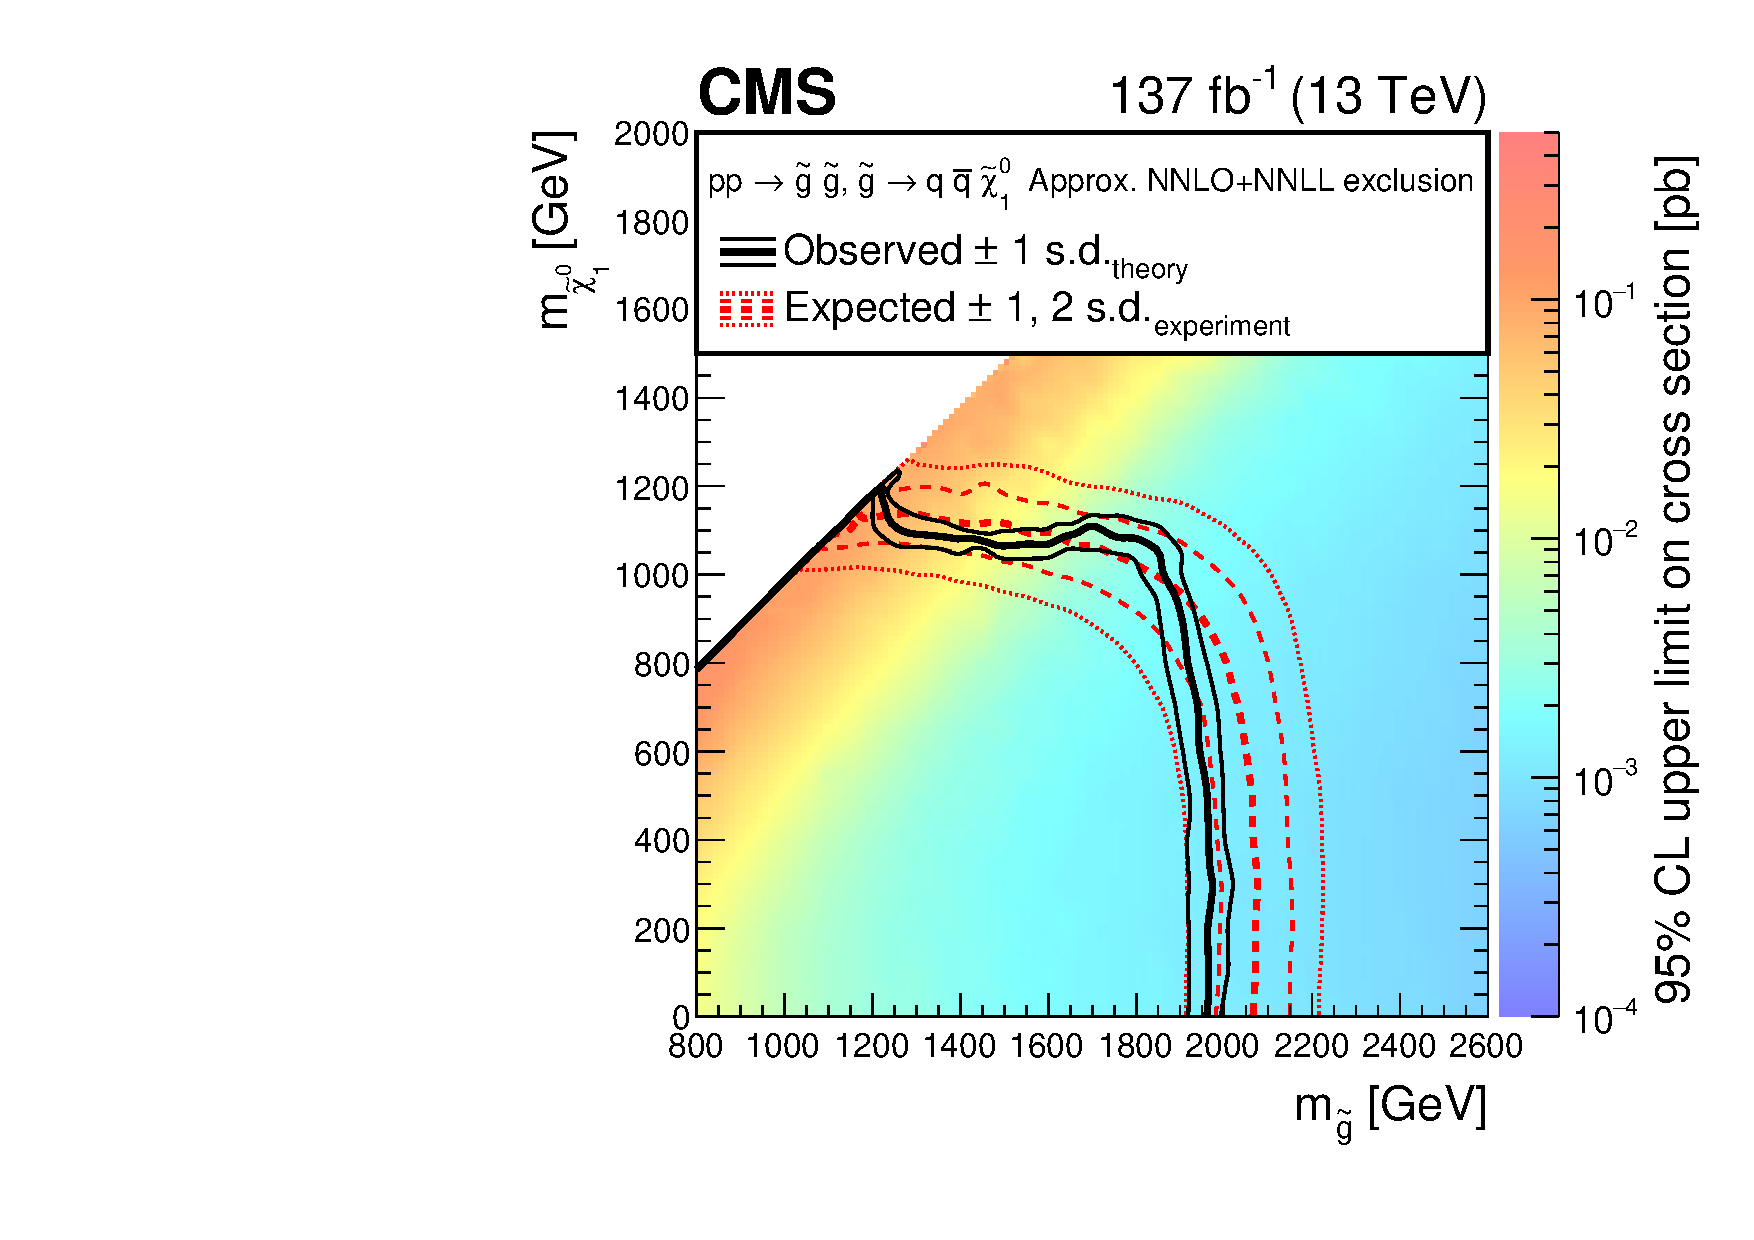
\includegraphics[width=0.48\textwidth]{figures/MT2_2019/Figure_011-a}\\
    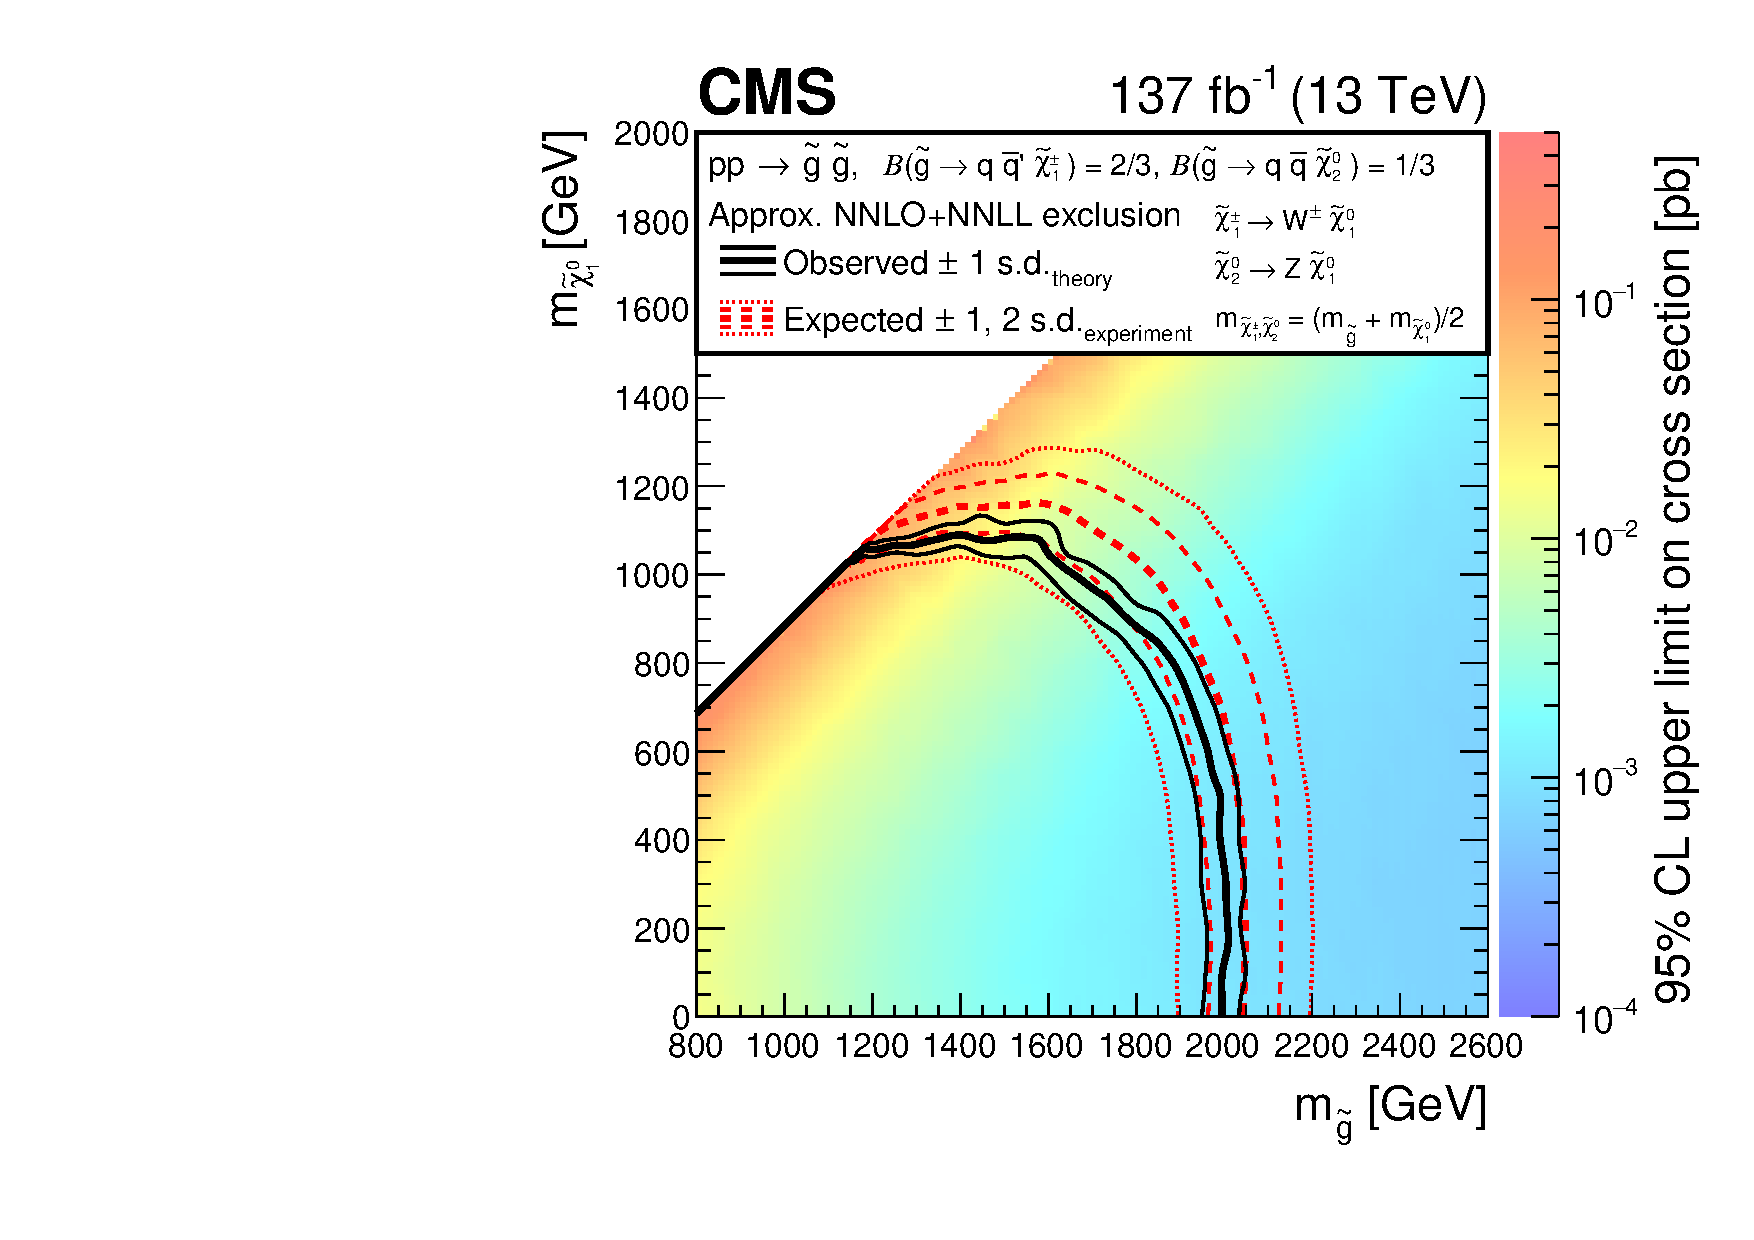
\includegraphics[width=0.48\textwidth]{figures/MT2_2019/Figure_011-b}
    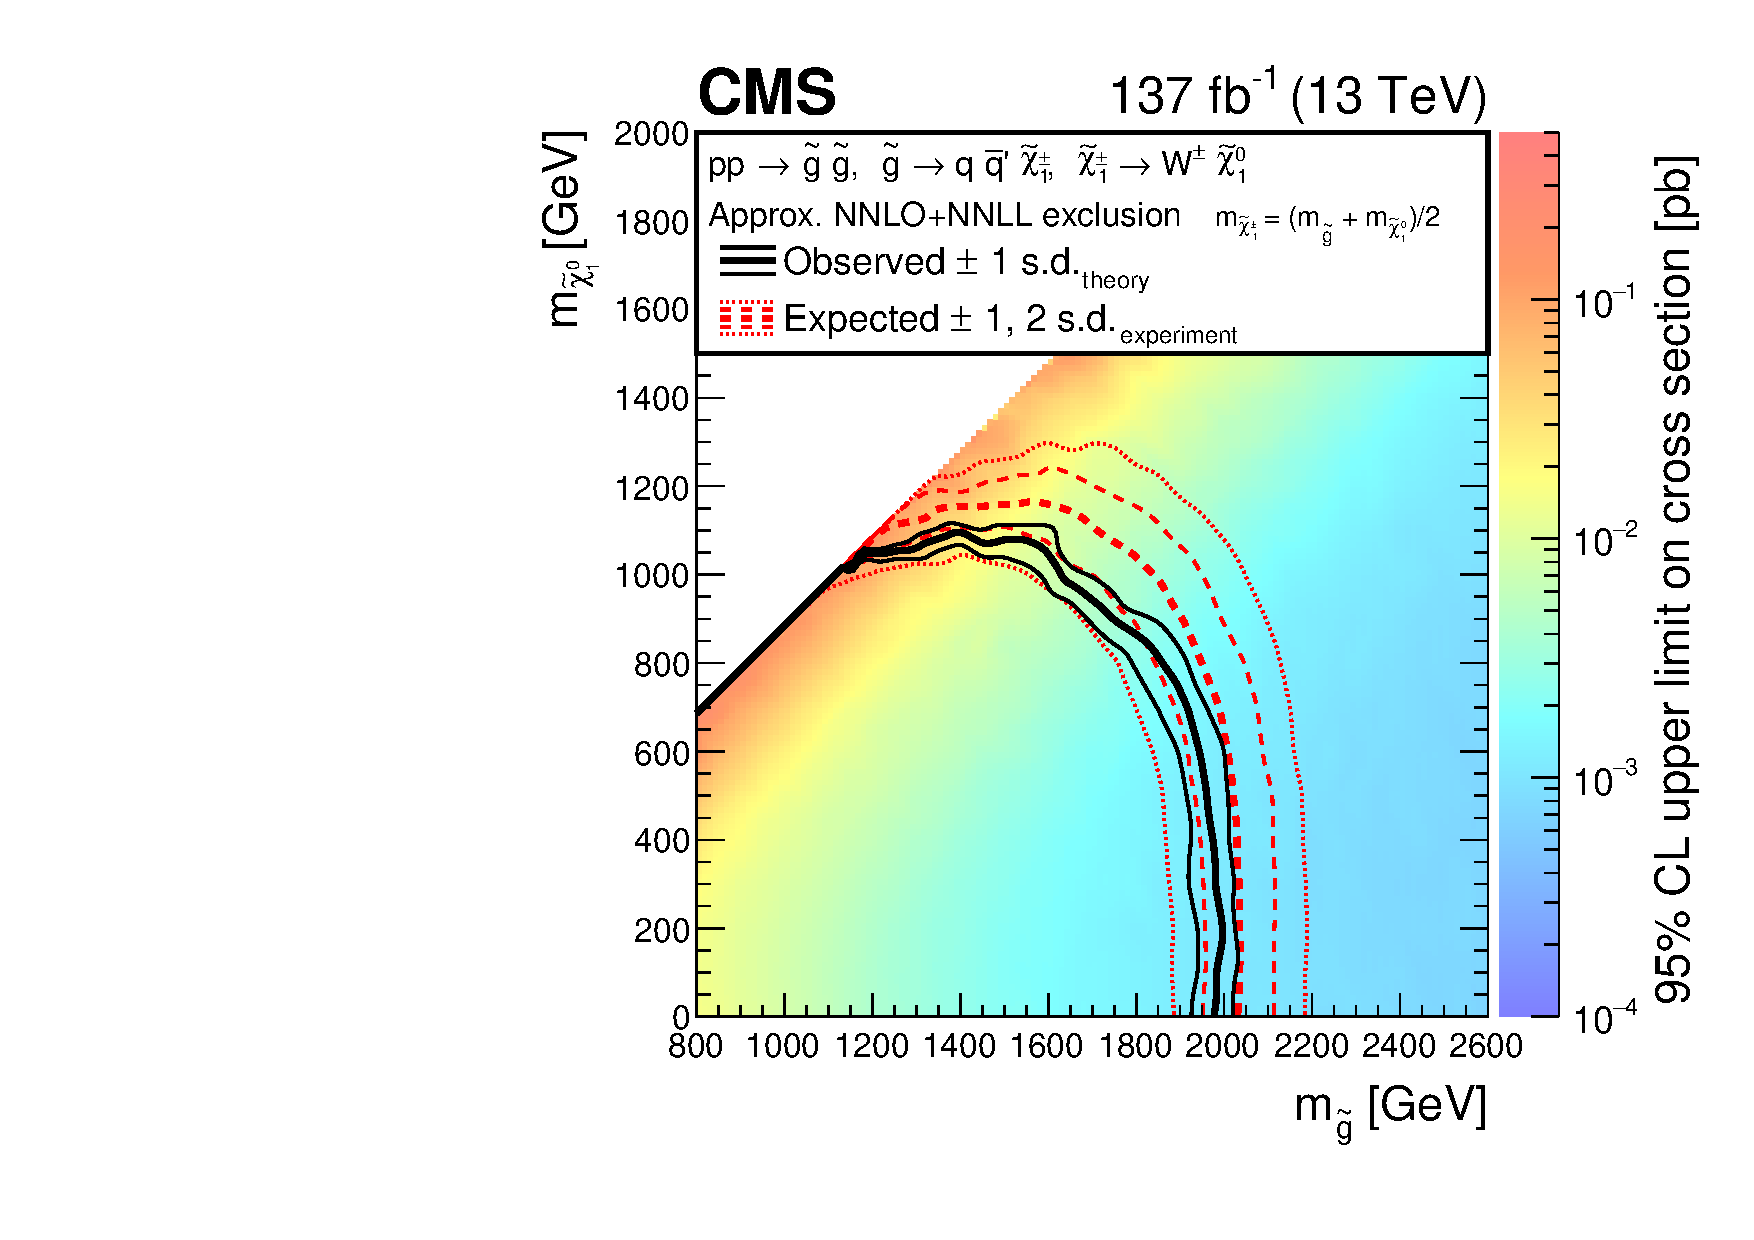
\includegraphics[width=0.48\textwidth]{figures/MT2_2019/Figure_011-c}
    \caption[Exclusion limits for gluino pair production and decay to light quarks.]{Exclusion limits at 95\% \CL for gluino pair production and decay to a pair of light quark jets and (upper) \lsp, (lower left) a democratic split between \lsp, \chitwo, which then decays to a Z boson and \lsp, and \chargino, which decays to a W boson and \lsp, and (lower right) \chargino then W and \lsp with 100\% branching fraction. Taken from \cite{MT2_2019}.}
    \label{fig:t5x}
\end{figure*}

\begin{figure*}[htbp]
  \centering
    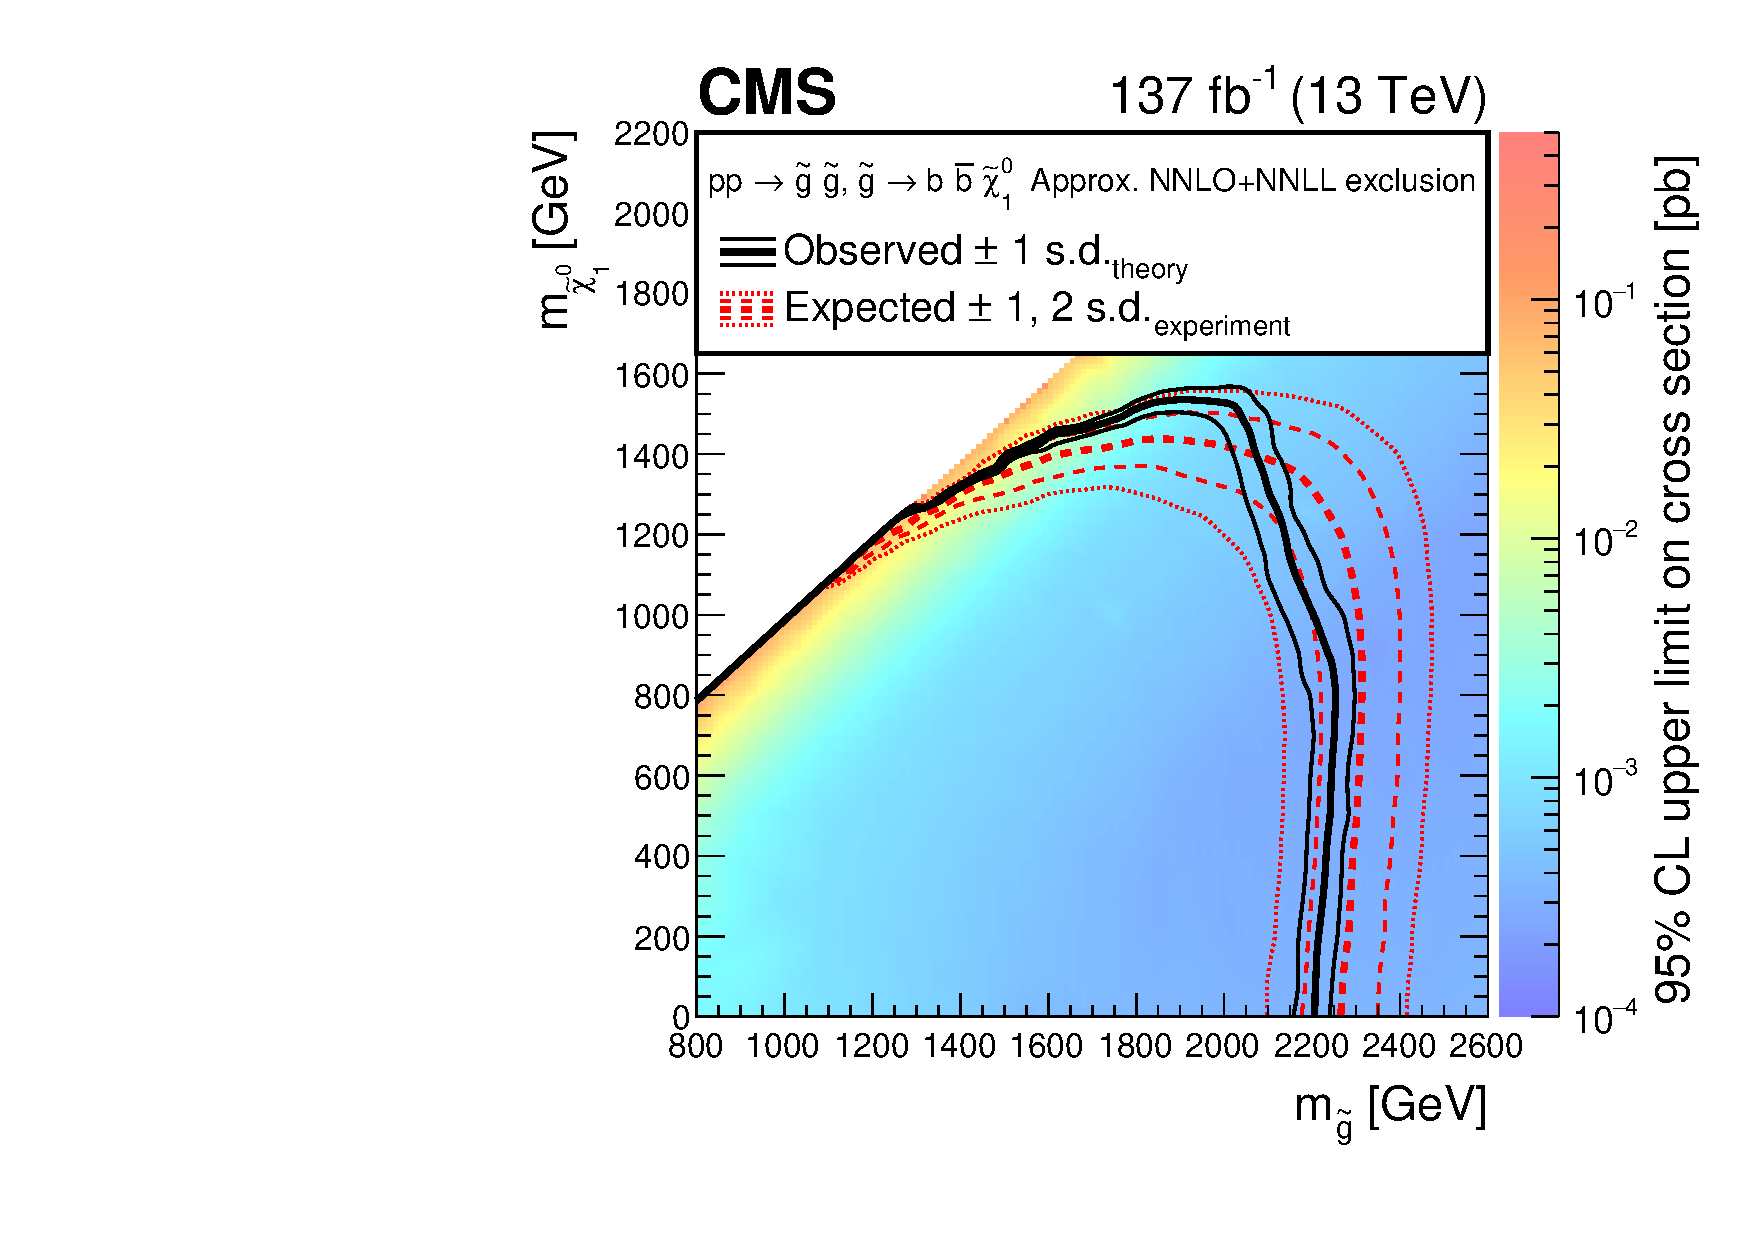
\includegraphics[width=0.48\textwidth]{figures/MT2_2019/Figure_012-a}
    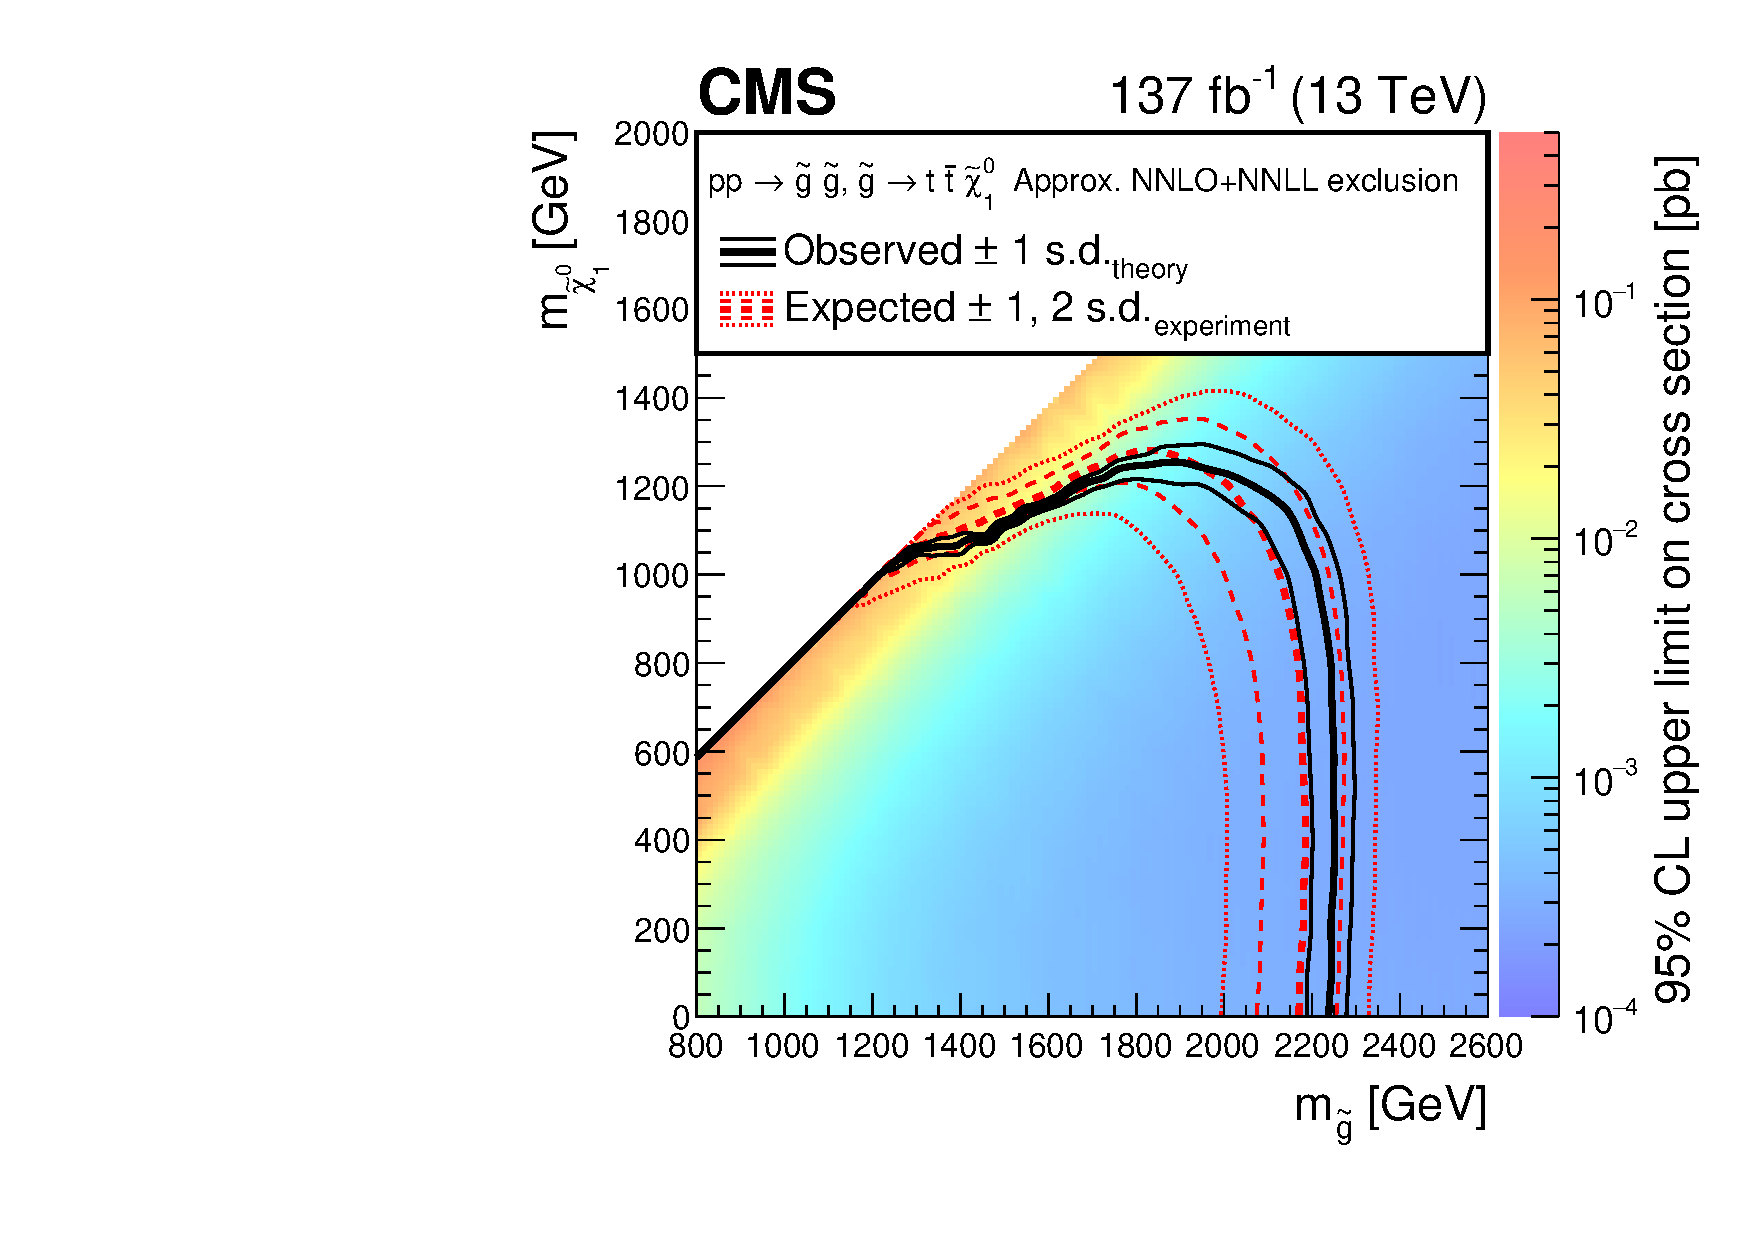
\includegraphics[width=0.48\textwidth]{figures/MT2_2019/Figure_012-b}
    \caption[Exclusion limits for gluino pair production and decay to bottom (left) and top (right) quarks.]{Exclusion limits at 95\% \CL for gluino pair production and decay to (left) bottom quarks and (right) top quarks. Taken from \cite{MT2_2019}.}
    \label{fig:t1x}
\end{figure*}

\begin{figure*}[htbp!]
  \centering
    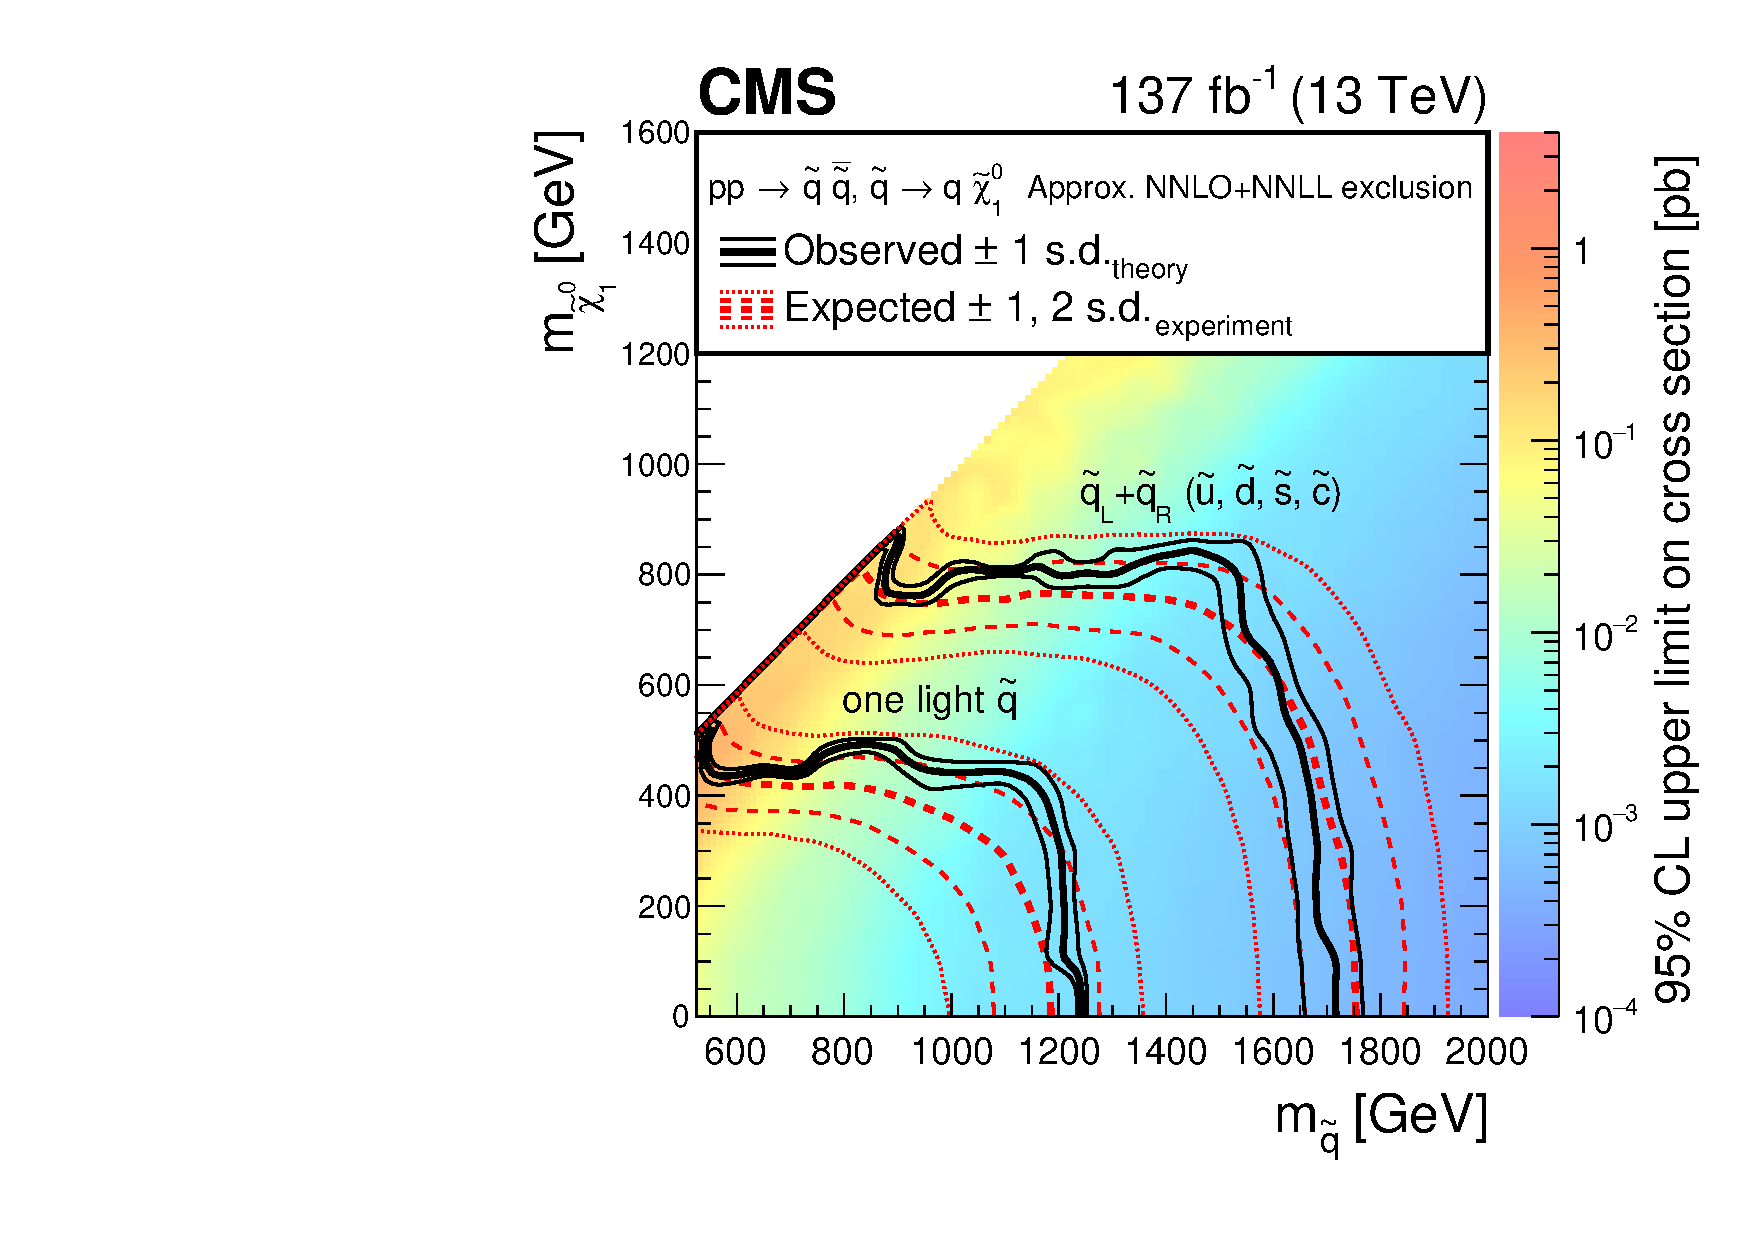
\includegraphics[width=0.48\textwidth]{figures/MT2_2019/Figure_013-a}
    \includegraphics[width=0.48\textwidth]{figures/MT2_2019/Figure_013-b}
    \includegraphics[width=0.48\textwidth]{figures/MT2_2019/Figure_013-c}
    \caption[Exclusion limit at 95\% \CL for (upper left) light-flavor squark pair production, (upper right) bottom squark pair production,
    and (lower) top squark pair production.]{Exclusion limit at 95\% \CL for (upper left) light-flavor squark pair production, (upper right) bottom squark pair production,
    and (lower) top squark pair production. Taken from \cite{MT2_2019}.}
    \label{fig:t2x}
\end{figure*}

\begin{figure*}[htbp!]
 \centering
   \includegraphics[width=0.49\textwidth]{figures/MT2_2019/Figure_014-a}
   \includegraphics[width=0.49\textwidth]{figures/MT2_2019/Figure_014-b}
   \includegraphics[width=0.49\textwidth]{figures/MT2_2019/Figure_014-c}
   \caption[Exclusion limit at 95\% \CL for top squark pair production for various decay modes of the top squark.]{
     Exclusion limits at 95\% \CL for top squark pair production and decay to (upper left) a bottom quark and \chargino, which subsequently decays to a W boson and \lsp, (upper right) either a bottom quark and \chargino or top quark and \lsp, or (lower) a charm quark and \lsp. Taken from \cite{MT2_2019}.}
   \label{fig:stop_other}
\end{figure*}

\begin{figure}[htbp]
 \centering
   \includegraphics[width=0.49\textwidth]{figures/MT2_2019/Figure_015}
   \caption[Exclusion limit at 95\% \CL for the mono-$\phi$ model.]{
     Exclusion limit at 95\% \CL for the mono-$\phi$ model. 
     Only the portion of the mass plane of phenomenological interest was simulated.
     The star indicates the original authors' proposed best fit mass point, which remains unexcluded.
     Taken from \cite{MT2_2019}.}
   \label{fig:monophilimits}
\end{figure}

\begin{figure*}[htbp]
 \centering
   \includegraphics[width=0.49\textwidth]{figures/MT2_2019/Figure_016-a}
   \includegraphics[width=0.49\textwidth]{figures/MT2_2019/Figure_016-b}
   \includegraphics[width=0.49\textwidth]{figures/MT2_2019/Figure_016-c}
   \caption[Upper limits at 95\% \CL on the leptoquark production cross sections as a function of leptoquark mass.]{
     Upper limits at 95\% \CL on the leptoquark production cross sections as a function of leptoquark mass. 
     Unlike the limits on supersymmetric models, in which the mass of \lsp is a free parameter, the limits on leptoquarks are 1-dimensional in the leptoquark mass since the neutrino masses are known to be approximately zero.
     Taken from \cite{MT2_2019}.}
   \label{fig:lqlimit}
\end{figure*}

  Figure~\ref{fig:t5x} shows the exclusion curves for gluino pair production and decay to light quarks (upper), light quarks and the Z boson (lower left), and light quarks and the W boson (lower right).
  Figure~\ref{fig:t1x} shows the exclusion curves for gluino pair production and decay to bottom (left) and top (right) quarks.

  Figure~\ref{fig:t2x} shows the exclusion curves for pair production of light-flavor squarks (upper left), bottom squarks (upper right), and top squarks in which the top squark decays to a top quark (lower). 
  The light-flavor figure contains two curves, one which assumes that there is only a single low mass light flavor squark, and another that assumes that there are eight light flavor squarks of (approximately) degenerate mass, which implies a production cross section eight times larger.
  The other top squark decay modes, in which the top decays to (upper left) a bottom quark and \chargino, which subsequently decays to a W boson and \lsp, (lower) a charm and \lsp, and (upper right) either \chargino and a bottom quark or \lsp and a top quark, are shown in Figure~\ref{fig:stop_other}.
  The charm decay channel is only shown for signal models with small mass splittings, as the top squark would strictly prefer to decay to a top quark and \lsp than to a charm quark and \lsp if kinematically allowed.

  Figure~\ref{fig:monophilimits} shows limits placed on the mono-$\phi$ model.
  Here, the horizontal axis is the mass of the singly-produced scalar $\phi$, and the vertical axis the mass of the invisible fermion $\psi$.
  A star indicates the mass point proposed by the original authors in \cite{monophi} as most phenomenologically interesting, which is not yet excluded.
  It is worth emphasizing that the background model is nevertheless consistent with data; this signal is simply very difficult to exclude with the \mttwo analysis methodology.
  To save computing resources, the mono-$\phi$ model is only simulated in the phenomenologically interesting subset of the mass plane, similarly to the top squark to charm model in Figure~\ref{fig:stop_other} (lower), hence the large white space beneath the considered range of masses.

  Figure~\ref{fig:lqlimit} shows limits for leptoquarks decaying to (upper left) a light flavor quark and neutrino, (upper right) a bottom quark and neutrino, and (lower) a top quark and neutrino.
  As the mass of the neutrinos, in contrast to the mass of \lsp, are known to be approximately zero, the leptoquark limits are one dimensional, in the leptoquark masses.

  The limits produced by this edition of the classic search improve upon the limits set by the previous edition \cite{MT2_2016} by hundreds of GeV, and in most cases are the strongest constraints on their respective signal models yet produced by any experiment.

  \subsection{Future of the Classic \mttwo Search} \label{sec:MT2future}

  The current limits produced by the classic \mttwo search are impressive, and are unlikely to improve much in the near future.
  The pair production cross section for squarks and gluinos drops rapidly with mass, as shown in Figure~\ref{fig:SUSYxsec}.
  Generically, a factor of 10 improvement in sensitivity is necessary to push the exclusion limits outward by around 500 GeV along the horizontal axis.
  At this mature statistical stage, a factor of 10 improvement in sensitivity requires a factor of 100 increase in the integrated luminosity, infeasible in the near future.
  Improvement along the \lsp axis is similarly difficult due to large backgrounds and low signal efficiency for models with small mass splittings.
  Therefore, attention in the near future will turn to other new techniques, one of which is discussed in the next section.

\section{Disappearing Tracks Search} \label{sec:distracks}

  \subsection{General Description} \label{sec:distracksdescription}

  As searches like that discussed in the previous section approach the practical limits of their sensitivities at the LHC, interest has grown in targeting plausible signals with peculiar features that more standard searches do not exploit.
  Among these features are those produced by relatively long-lived particles (LLPs) that do not decay promptly at the collision point, but instead travel a macroscopic distance into the detector before decaying. 
  An overview of some possibilities in the context of supersymmetry is provided in \cite{LLPsAtLHC}.

  One of these signatures is a disappearing track, produced when a charged particle, such as \chargino, travels into the tracker, then decays to an invisible particle, such as \lsp, with a mass so nearly equal to that of the decaying charged particle that the visible products of the decay are too low energy to be reconstructed. 
  The supersymmetric parameter space is vast and there is no way to know which if any version of supersymmetry is realized in nature, but models including LLPs that would produce disappearing tracks at CMS have been argued to be especially plausible on theoretical grounds \cite{distracks1, distracksAMSB, AMSBlifetime}.
  The \mttwo analysis is already well-optimized for all-hadronic supersymmetry, so it is natural to search for all-hadronic decays of these models by extending it with a disappearing track search.
  This extension begins with exactly the same set of selected events as the classic search, and then further selects the subset of events possessing a disappearing track.

  \subsection{Challenges} \label{sec:distrackschallenges}

  The disappearing tracks search must confront a pair of significant challenges.

  First, the background (see Section~\ref{sec:distracksbg}) entirely consists of events in which reconstruction failed, analogous to the classic search's detector mismeasurement background that was discussed in Section~\ref{sec:MT2QCD}, and is difficult to understand and estimate for many of the same reasons.
  Simulation cannot be trusted to account for all of the detector details that lead to extremely rare reconstruction errors.
  While the classic search can mitigate the impact of this issue with selections that make the mismeasurement background subdominant compared to the better understood neutrino backgrounds, this is not possible for the disappearing track search since no such genuine background exists.
  Moreover, since the background is dependent on details of the detector, it is strongly affected when these details change.
  Most prominently, the CMS pixel detector was entirely replaced between the 2016 and 2017 data taking periods \cite{phase1}, and this profoundly affected CMS track reconstruction, to the extent that the disappearing track search must treat the 2016 data entirely separately from the 2017 and 2018 data.
  The detector's state also evolves more subtly over the data taking period, due in large part to inevitable radiation damage, and the analysis must track, study, and account for the effect of this evolution on the occurrence of disappearing tracks.
  
  Second, disappearing tracks are extremely rare.
  This is of course one of the motivations for the disappearing tracks extension---they are a powerful tool to discriminate between background and likely signal events---but it also makes them difficult to study.
  
  Nevertheless, the disappearing tracks search produced a data-driven background estimation procedure, described in Section~\ref{sec:distracksbgest}, that was successfully validated in data, and achieved the best sensitivity to disappearing tracks in supersymmetric models to date.
  
  \subsection{Signal Models} \label{sec:distrackssig}

  \begin{figure*}[htbp]
    \centering
    \includegraphics[width=0.55\textwidth]{figures/chargino_lifetime.png}
    \caption[Lifetime of \chargino as a function of mass splitting.]{
      The rest frame lifetime of \chargino as a function of the \chargino-\lsp mass splitting. 
      The lifetime is macroscopic for mass splittings less than 1~GeV in a broad class of supersymmetric models, a regime that is realized  when the superpartner mass scale is much larger than the Standard Model mass scale. 
      This mass splitting is so small that the charged daughter of \chargino decay is too low energy for track reconstruction.
      Thus, \chargino lives long enough to produce a short track in the CMS tracker, then disappears when it decays to \lsp and a lost charged daughter.
      For mass splittings less than $M_{\pi} \approx 140$~MeV, indicated on the plot, the lifetime of \chargino is so long that it typically does not decay inside the tracker.
      As a result, the sweet spot for the disappearing tracks search is mass splittings on the order of hundreds of MeV.
      The discontinuity at a mass splitting of 1.4~GeV is not physical.
      Taken from \cite{AMSBlifetime}.}
    \label{fig:charginolifetime}
  \end{figure*}

  For the class of supersymmetric models discussed in \cite{distracksAMSB} \& \cite{AMSBlifetime}, the relative mass splitting of \chargino and \lsp is proportional to $(M_{W}/\mu)^4$, where $\mu$ is a parameter that roughly represents the energy scale of supersymmetry.
  Non-observation of superpartners thus far at the LHC suggests that $\mu$ is probably large, on the order of TeV, implying $(M_{W}/\mu)^4 < 10^{-4}$.
  Such a tiny mass splitting leads to a remarkably long \chargino lifetime, shown in Figure~\ref{fig:charginolifetime}.

  \begin{figure*}[htbp]
    \centering
    \includegraphics[width=0.3\textwidth]{figures/MT2_2019/Figure_010-a}
    \includegraphics[width=0.3\textwidth]{figures/MT2_2019/Figure_010-b}
    \includegraphics[width=0.3\textwidth]{figures/MT2_2019/Figure_010-c}
    \caption[Diagrams for (left) gluino, (center) light-flavor squark, and (right) top squark pair production, in which the gluinos and squarks can decay via a long-lived \chargino]{Diagrams for (left) gluino, (center) light-flavor squark, and (right) top squark pair production, in which the gluinos and squarks can decay via a long-lived \chargino. In this analysis, the gluino is taken to decay with branching fraction $\frac{1}{3}$ each to the \lsp, \chim, and \chip. Squarks decay with branching fraction $\frac{1}{2}$ each to the \lsp and the \chargino allowed by charge conservation. The \chargino mass is greater than the \lsp mass by hundreds of MeV, so that the charged product of the \chargino decay is too soft to be detected. Taken from \cite{MT2_2019}.}
    \label{fig:charginodiags}
  \end{figure*}
  
  Motivated by these models, the disappearing track seach considers signals that include an intermediate \chargino in the superpartner decay chain, similar to the models in Figure~\ref{fig:susyproduction} (upper right, lower left, and lower center) considered by the inclusive search.
  The \chargino is taken to be long-lived, only hundreds of MeV more massive than \lsp.
  Specifically, the rest frame \chargino lifetime, $\tau_0$, is varied from $c\tau_0 = 1$~cm to $c\tau_0 = 2000$~cm.
  This range of lifetimes is selected because the CMS tracker extends from $r\approx10$~cm to $r\approx 100$~cm, and a significant fraction of \chargino decays must occur inside the tracker for the disappearing track search to have meaningful sensitivity.
  If the decay occurs outside the tracker, the track does not disappear.
  The full set of models considered is shown in Figure~\ref{fig:charginodiags}.
  
  In the model at left, gluinos are pair-produced and decay with equal probability either to \chip, \chim, or \lsp, and light-flavor quarks.

  In the central model, light flavor squarks are pair-produced and decay with equal probability either to the allowed charge of \chargino, or to \lsp, and a light-flavor quark.

  In the model at right, top squarks are pair-produced and decay with equal probability either to the allowed charge of \chargino, or to \lsp, and a bottom quark.

  \begin{figure}[h!]
    \centering
    \includegraphics[width=0.85\textwidth]{figures/reliso_SvsB.pdf}
    \caption[Comparison of signal and background Short Track relative isolation distributions.]
            {Disappearing tracks produced by \chargino decays (black triangles) tend to be much more isolated than disappearing tracks in background events (red squares).
              All selections listed in Table~\ref{tab:shorttrackselection} are applied except the isolation selections.
              The last bin is an overflow bin, containing every track failing the relative isolation selection.
              The events containing those tracks will either populate control regions, or be rejected entirely, as described in Section~\ref{sec:distracksbgest}.
              Additional material from \cite{MT2_2019}.}
            \label{fig:distracksisolation}
  \end{figure}  

  The disappearing tracks produced by \chargino decays tend to be very high quality and highly isolated (shown in comparison with background in Figure~\ref{fig:distracksisolation}), with negligible energy deposits in any of the calorimeter cells along the track's extrapolated path.
  The quality metrics in this context include the track's impact parameter with respect to the primary vertex, the size of the uncertainty in the track's assigned \pt, and the number of tracker layers in which the track failed to leave a hit when one would be expected.
  Alongside isolation, shown in Figure~\ref{fig:distracksisolation}, these quality metrics allow for signal-like disappearing tracks to be distinguished from disappearing tracks that are very likely to be due to a reconstruction error.
  This forms the basis of the background estimate described in Section~\ref{sec:distracksbgest}.

  \subsection{Backgrounds} \label{sec:distracksbg}

  In contrast to the classic search, there are no irreducible disappearing track backgrounds produced by the Standard Model.
  However, there are a number of detector reconstruction issues that can lead to apparent disappearing tracks, many of which can be greatly or even entirely rejected by various cleaning selections.

  Of the near-entirely reducible backgrounds, the largest before cleaning is that produced by electrons undergoing unusually strong bremsstrahlung inside the tracker, effectively converting the electron into a photon.
  While electrons are charged and therefore produce tracks, photons are neutral and do not.
  So, these tracks disappear, but can normally be rejected due to large photon energy deposits in the electromagnetic calorimeter cells to which the track extrapolates.
  However, some ECAL cells do not perform well for a variety of reasons and may fail to register the photon energy deposits, and so fail to veto the disappearing track.
  Fortunately, the majority of the ECAL performs well enough to make this background significant only for tracks extrapolating to defective cells.

  Defective cells are mapped and vetoed using a tag-and-probe strategy, in which a PF electron ``tag'' identifies potential $Z\rightarrow e^+e^-$ events, and a disappearing track of opposite charge serves as the ``probe.''
  If an event contains exactly one PF electron, the event is searched for a disappearing track of opposite charge, under the hypothesis that the event was in fact $Z\rightarrow e^+e^-$ and the second electron was not successfully reconstructed due to the conversion process described above.
  If such a track is found and the invariant mass of the electron-disappearing track pair is consistent with the mass of the Z boson, the region of the ECAL to which the disappearing track extrapolated is deemed faulty.
  $Z\rightarrow e^+e^-$ events are sufficiently common that the map of faulty ECAL cells can be assembled as a function of time.
  As expected, the performance of the ECAL steadily degrades over time, so that the fraction of the ECAL that must be vetoed increases from 2016 to 2017 to 2018.
  This veto essentially entirely rejects the electron conversion background, but at a price. 
  It is the single largest cause of signal inefficiency, as 15-20\% of signal disappearing tracks point, by chance, into vetoed regions of the ECAL.

  Another, much smaller reducible background is produced by the decay of strange baryons, including the $\Xi^{\pm}$, $\Sigma^{\pm}$, and $\Omega^{\pm}$.
  These baryons have lifetimes in the proper range to produce tracks 10s of centimeters long, before decaying with a small mass splitting to a neutral baryon and a charged daughter that is sometimes low enough \pt to escape reconstruction.
  While these tracks disappear from the perspective of the tracker and the ECAL, the neutral baryon is still detectable in the hadronic calorimeter via its nuclear interactions, which allows for efficient rejection of this background.
  Additionally, strange baryons are almost always found inside jets, so the vast majority of their tracks can be vetoed on the basis of isolation.
  Even so, a region of the HCAL with known performance issues in 2018 showed significantly increased disappearing track counts that required it to be vetoed, likely in part because of this background.

  The final two backgrounds are fake tracks and mesons, mostly pions, that undergo nuclear interactions in the tracker, neither of which can be entirely rejected.
  
  Fake tracks are tracks comprised of hits that are not all associated to the same genuine particle.
  The probability that track reconstruction produces a fake track is small, and can be suppressed by requiring that tracks pass a sophisticated selection called high purity, as shown in Figure~\ref{fig:trackfakerate} for the 2016 tracker \cite{cmstracking}, which improved after the pixel tracker upgrade between 2016 and 2017 \cite{cmstrackingphase1} as shown in Figure~\ref{fig:16vs17}~(right).
  Furthermore, the probability that more than 3 or 4 unassociated hits will be strung together into a track is negligible, limiting the fake track background to very short tracks.
  It is also rare for unassociated hits to lie on a tight, relatively straight line; instead, they tend to be somewhat scattered.
  Therefore, fake tracks also tend to assigned low \pt, since low energy track have greater curvature in the detector's magnetic field.
  The disappearing tracks analysis considers only tracks with $\pt > 15$~GeV in part to avoid the majority of the fake track background, and divides tracks into low and high \pt bins partly in order to maintain a relatively fake-free high \pt region.

  While the fake track background is limited to shorter tracks, the meson background is not and so constitutes the dominant longer disappearing track background.
  This background is generated when a meson undergoes a nuclear interaction inside the tracker, and showers in such a way that no single charged daughter is high enough energy to be reconstructed as a track, and any neutral products are sufficiently low energy or widely scattered that calorimeter deposits are insufficient to reject the track.
  While it is merely unusual for a meson to undergo a nuclear interaction in the tracker as shown in Figure~\ref{fig:pionsurvival}, a shower leaving no detectable products is extraordinarily rare, occurring only a handful of times across three years of data taking.
  Mesons tend not to be isolated, allowing most of this background to be distinguished from signal-like tracks, but with one major exception.
  The $\tau$ lepton, almost always isolated when produced in the hard interaction, undergoes the decay $\tau^{\pm} \rightarrow h^{\pm}\nu$ for some meson $h^{\pm}$, almost always a $\pi^{\pm}$, with probability approximately 11.5\% \cite{pdg}.
  In this decay, the $\pi^{\pm}$ effectively inherits the isolation of the $\tau$.
  If this $\pi^{\pm}$ undergoes the rare shower described above, it produces an isolated disappearing track of potentially significant length, scarcely distinguishable from a signal track.
  For this reason, observation of even a relatively long, isolated, maximally signal-like disappearing track is not itself sufficient to discover a signal. 
  An estimate of the background's rate is necessary, to allow a comparison to the observed frequency of disappearing tracks.

  \subsection{The Short Track Selection and Data-Driven Background Estimate} \label{sec:distracksbgest}

  The two surviving disappearing track backgrounds, fake tracks and lost pions, are both produced by extremely rare failure modes of the detector.
  A data-driven background estimate is mandatory, as replicating such pathological edge cases is beyond the capabilities of any feasible simulation.
  This requires definition of signal-depleted control regions that can be used to measure the rate at which known physics processes produce disappearing tracks.
  As discussed with respect to the classic search's mismeasurement background in Sections~\ref{sec:MT2QCD}~\&~\ref{sec:RandS}, events with low \mttwo are extremely background dominated.
  Low \mttwo events compose one such control region.
  This dependence on \mttwo to define a signal-depleted control region restricts the disappearing track search to multijet events, as no comparably powerful discriminant is known for monojet events.
  In high \mttwo events, properties of the disappearing tracks themselves are used to divide events with signal-like disappearing tracks, called Short Tracks (ST), and background-like disappearing tracks, called Short Track Candidates (STCs), into ST signal regions and STC control regions.
  The ST and STC selections are summarized in Table~\ref{tab:shorttrackselection}.
  Signal disappearing tracks pass this selection in simulation with efficiency between 50\% and 65\%, while only around 1 in 1000 to 1 in 10,000 background events passing the baseline selection of the \mttwo analysis possess a track passing the ST selection.
  The STC selection is not maximally background-like; rather, it selects tracks that nearly pass the ST selection, but are not STs.
  Instead, these tracks pass only a relaxed version of the ST selection.
  This choice ensures that STCs are as closely linked to STs produced by background as possible, without including a significant amount of true signal tracks.
  Only a few per cent of signal tracks are selected as STCs, usually due to an unlucky overlap with a jet causing a high isolation value as shown in Figure~\ref{fig:distracksisolation}, but STCs are a few times more common in background events than STs.

  The selections relaxed for STCs with respect to the ST definition can be grouped into two categories, those concerned with track quality, which are loosened by a factor of 3, and with isolation, which are loosened by a factor of 6.
  The specific track quality selections affected are the impact parameter, both along the beam axis and in the transverse plane, and the \pt error $\sigma(\pt)$.
  All isolation selections are loosened.  

  \begin{table}[htbp]
    \caption[Table of ST and STC selections.]
            {Selection requirements for STs and STCs.
              Some requirements differ for tracks of different lengths; the length categories are described in Section~\ref{sec:distracksbinning}.
              For the subset of medium (M) length tracks that have just four tracking layers with a measurement, the minimum required number of layers of the pixel tracking detector with a measurement is three ($\dagger$).
              The selected tracks are required not to overlap with any identified electrons or muons, of any quality.
              The selected tracks are as well required to not be identified as PF candidates, 
              and not to overlap with other tracks with $\pt>15\GeV$, even if those tracks are not associated to PF candidates.
              The table also reports the factor by which a selection is relaxed to define STCs, when applicable.
              If no factor is reported, the requirement is not relaxed for the selection of short track candidates.
              \label{tab:shorttrackselection}}
    \small
    \centering
    \begin{tabular}{l | l | c | c}
      \hline
      Observable                            & Selection         & Track length          & STC factor\\
      \hline
      \pt [GeV]                                            & $> 15$         & All                     & \\
      $\left|\eta\right|$                                 & $< 2.4$ and not $1.38 < \left|\eta\right| < 1.6$ & All & \\
      %  & not $1.38 < \left|\eta\right| < 1.6$           &  & \\
      \hline
      $\sigma(\pt)$ / $\pt^2$ [GeV$^{-1}$]                          & $< 0.2$; $< 0.02$; $< 0.005$           & P; M; L                        & $\times 3$ \\
      $d_{\mathrm{xy}}$ (from primary vertex) [cm]                                            & $< 0.02$ ( $< 0.01$ )           & P ( M, L )                       & $\times 3$  \\
      $d_{\mathrm{z}}$ (from primary vertex) [cm]                                             & $< 0.05$           & All                     & $\times 3$  \\
      \hline
      Neutral isolation ($\Delta R < 0.05$) [GeV]                          & $< 10$         & All                     & $\times 6$  \\
      Neutral isolation / \pt                & $< 0.1$            & All                     & $\times 6$  \\
      Isolation ($\Delta R < 0.3$) [GeV]                             & $< 10$         & All                     & $\times 6$  \\
      Isolation / \pt                          & $< 0.2$            & All                     & $\times 6$   \\
      \hline
      Number of pixel layers             & $\geq 3$ ( $\geq 2$ )           & P, M$^{\dagger}$ ( M, L )                 & \\
      Number of tracker layers             & $\geq 3$; $<7$; $\geq7$           & P; M; L                 & \\
      Number of lost inner hits                           & $= 0$              & All                     & \\
      Number of lost outer hits                           & $\geq 2$           & M, L                     & \\
      \hline
      Is a PF candidate?                                    & No                 & All                     & \\  
      PF lepton veto ($\Delta R < 0.1$)           & Yes   & All                     & \\
      Lepton veto ($\Delta R < 0.2$)              & Yes   & All                     & \\
      Track veto ($\Delta R < 0.1$)               & Yes   & All                     & \\
      Bad calorimeter module veto                 & Yes                 & All                     &  \\
      \Mt(track, $\vec{\met}$) [GeV]                     & $> 100$, if $\pt < 150\GeV$ & L  &  \\
      \hline
    \end{tabular}
  \end{table}

    \begin{figure}[h!]
      \centering
      \includegraphics[width=0.85\textwidth]{figures/sigeff_bylength.pdf}
      \caption[Signal efficiency with respect to the short track selection.]
              {The signal efficiency with respect to the full short track selection after selecting events passing the baseline kinematic signal region selection.
                Additional material from \cite{MT2_2019}.}
      \label{fig:distrackssigeff}
    \end{figure}  

    The efficiency for signal tracks to pass this selection is high, 50--65\%, as shown in Figure~\ref{fig:distrackssigeff}.

    \subsubsection{Binning} \label{sec:distracksbinning}

    The background for shorter disappearing tracks is dominated by fakes, while the background for longer disappearing tracks is dominated by lost pions.
    Additionally, signals with different LLP lifetimes produce tracks of different lengths.
    Thus, binning the signal region by track length allows backgrounds of different origins to be segregated in different bins, and maximizes sensitivity to a variety of signal lifetimes.
    The disappearing track search adopts 3 categories of tracks length.
    \begin{itemize}
      \item Pixel-only (P) tracks have hits only inside the pixel tracker. Fakes dominate the background. In 2017 and 2018 data, these tracks are further subdivided into pixel tracks with hits in 3 distinct layers (P3) and pixel tracks with hits in 4 distinct layers (P4).
      \item Medium length (M) tracks have hits in fewer than 7 distinct layers, but have at least one hit outside the pixel detector. Lost mesons dominate the background.
      \item Relatively long (L) tracks have hits in 7 or more distinct layers, but still disappear, having missing expected hits in at least the two outermost layers of the tracker. Lost mesons dominate the background, and the better opportunity to measure the track allows for an especially tight selection, allowing for extremely strong background suppression.
    \end{itemize}
    Additionally, P and M tracks are divided into tracks with $15 < \pt < 50$~GeV (``lo'') and tracks with $\pt \geq 50$~GeV (``hi'').
    Most background falls into the low \pt bins, and signals generically populate the high \pt bins, making the high \pt bins the drivers of sensitivity to most signals.
    This division is not adopted for L tracks, as statistics are too low to allow further division of that population of tracks.

    Finally, events are binned based on the global event kinematics, using \njet\, and \Ht, again partly to segregate backgrounds produced by different signals and partly to enhance sensitivity to a variety of signal models.
    The \njet\, bins are $2 < \njet \leq 3$ (denoted by a trailing L, targeted at squark production), and $\njet > 4$ (H, targeted at gluino production).
    The \Ht bins are $250 < \Ht < 575$~GeV (denoted by a leading ``L''), $575 \leq \Ht < 1200$~GeV (``M''), and $\Ht \geq 1200$~GeV (``H'').
    For events with L length tracks, the L and M \Ht bins are merged into ``LM'' to preserve statistics.

    For example, the ``L HLM'' region is populated by events with L length tracks, with $\njet \geq 4$ and $\Ht \geq 1200$~GeV.
    The ``M LM lo'' region is populated by events with M length tracks of $15 < \pt < 50$~GeV, with $2 \njet \leq 3$ and $250 < \Ht < 575$~GeV.

    The STC control region binning mirrors the ST signal region, with each STC bin mapping to a corresponding ST bin.

    \subsubsection{Short Track Candidates and \fshort} \label{sec:fshort}

    The background estimation procedure makes use of the ratio of the counts of STs and STCs, called \fshort,
    \begin{equation}
      \fshort = \frac{N_{\mathrm{ST}}}{N_{\mathrm{STC}}}.
      \label{eqn:fshort}
    \end{equation}
    This ratio is measured in events with $60 < \mttwo < 100$~GeV, as these events are so background-dominated that even STs are assuredly background-dominated.
    A separate \fshort is measured for every bin, except that the measurement is inclusive in \Ht, exploiting an empirical invariance of \fshort with respect to \Ht to improve the statistical precision of the measurement.
    The ratio is then applied at high \mttwo to estimate the number of signal-like STs produced by background, $N_{\mathrm{ST}}^{\mathrm{B}}$, using the number of STC events observed in the corresponding control region, $N_{\mathrm{STC}}^{\mathrm{Obs}}$,
    \begin{equation}
      N_{\mathrm{ST}}^{\mathrm{B}} = \fshort N_{\mathrm{STC}}^{\mathrm{Obs}}.
      \label{eqn:fshortest}
    \end{equation}
    This estimate is correct up to statistical fluctuations, subject to the assumption that \fshort is invariant with respect to \mttwo, an assumption which is validated in data in the next subsection.
    Even without this explicit validation, there is no reason to expect that a ratio based on track-level observables, namely the impact parameter, \pt error, and isolation, ought to be sensitive to a global event kinematic variable like \mttwo.
    By tethering the background estimate to the observed count of STCs in data, the analysis is able to remain agnostic of the details of background disappearing track production.

    \subsubsection{Validation} \label{sec:distracksvalidation}

    \begin{figure}[h!]
      \centering
      \includegraphics[width=0.85\textwidth]{figures/MT2_2019/Figure_004-a.pdf}
      \includegraphics[width=0.85\textwidth]{figures/MT2_2019/Figure_004-b.pdf}
      \caption[Validation of the disappearing tracks background estimate in (upper) 2016 and (lower) 2017--2018 data.]
              {Validation of the disappearing tracks background estimate in (upper) 2016 and (lower) 2017--2018 data.
                There are no discrepancies inconsistent with statistical fluctuations.
                To be conservative, a systematic uncertainty (gray) is assessed region-by-region to account for any discrepancy greater than 1 statistical standard deviation (blue).
                Dotted vertical lines group bins that use the same measured value of \fshort, because they differ only in \Ht.
                Taken from \cite{MT2_2019}.}
      \label{fig:distracksval}
    \end{figure}  

    The \fshort-based estimate of background ST production relies on the invariance of \fshort with respect to \mttwo. 
    The \fshort ratio is measured at $60 < \mttwo < 100$~GeV, a background-dominated region, and applied in the $\mttwo > 200$~GeV signal region. 
    In Figure~\ref{fig:distracksval}, the invariance of \fshort with respect to \mttwo is validated in the intermediate region, $100 < \mttwo < 200$~GeV, in both 2016 and 2017--2018 data, by carrying out the background estimation procedure as used for the signal region in this \mttwo sideband.
    There are no discrepancies inconsistent with statistical fluctuations, so the estimate is considered validated.
    To be conservative, a systematic uncertainty is assessed bin-by-bin that is no less than the statistical uncertainty, to prevent any cases of accidental closure, and as large as is necessary to cover any observed discrepancy larger than 1 standard deviation of statistical uncertainty.

  \subsection{Systematics} \label{sec:distrackssysts}

  \begin{table}[htb!]
    \centering
    \topcaption[Table of uncertainties affecting the disappearing tracks background prediction.]{\label{tab:distracksyst}
      Summary of systematic uncertainties in the disappearing track background prediction, together with their typical size ranges across the search bins.
      The systematic uncertainties arising from the assumption of kinematic invariance of \fshort and from the validation of the background prediction are always taken
      to be at least as large as the statistical uncertainties on the measured values of  \fshort and on the background prediction in the validation region,
      respectively.
      Taken from \cite{MT2_2019}.
    }
    \begin{tabular}{ l  c }
      \hline
      Source & Range [\%] \\
      \hline
      Limited size of data control samples (high \mttwo STC counts) & 1--100\\
      Limited size of data \fshort measurement samples (low \mttwo disappearing track counts) & 5--45\\
      Kinematic invariance of \fshort & 10--80\\
      Validation of background prediction & 25--75\\
      \hline
    \end{tabular}
  \end{table}
  
  The uncertainties uniquely affecting the disappearing tracks the background prediction, in addition to those obtained from the validation region, are summarized in Table~\ref{tab:distracksyst} together with their typical size ranges across the search bins.

  The first two uncertainties are purely statistical and dominate the total uncertainty. 

  The kinematic invariance of \fshort is checked by varying the \Ht and \met definitions of the \fshort measurement region.
  Any uncertainty greater than 1 statistical standard deviation is covered by applying a systematic, just as for the validation region systematic.
  Although the relative uncertainties thus assessed can be large, this is an artifact of extremely low statistics.
  Discrepancies easily consistent within 2 statistical standard deviations can nonetheless lead to assessment of a large relative systematic uncertainty.
  Still, these uncertainties are applied to ensure that the disappearing tracks search is conservative.

  As for the classic search, the disappearing tracks signal simulation is subject to extra uncertainties, all of which are shared except the uncertainties assessed to cover the reconstruction of signal disappearing tracks, produced by decaying \chargino.
  There are three such uncertainties.

  First, fast simulation is used for signals simulated in 2017 and 2018 conditions. 
  The selection efficiency for signal tracks in fast simulation differs slightly from full simulation, and so a systematic is assessed to cover the difference.

  A 10\% uncertainty is assessed to cover any potential mismodeling of how efficiently the detector would reconstruct tracks from a long-lived \chargino.
  This is half the difference between unity and the observed efficiency in simulation, for \chargino decays in the regions of the detector that ought to be able to reconstruct the tracks successfully.

  Finally, an uncertainty of 1.5\% is assessed to cover observed differences between full simulation and fast simulation in how often a \chargino that reaches the muon chamber is falsely reconstructed as a muon, triggering the lepton veto.

  \subsection{Results} \label{sec:distracksresults}

  \begin{figure}[h!]
    \centering
    \includegraphics[width=0.85\textwidth]{figures/MT2_2019/Figure_006-a.pdf}
    \includegraphics[width=0.85\textwidth]{figures/MT2_2019/Figure_006-b.pdf}
    \caption[Comparison of the predicted background and observed data events in the disappearing track search for (upper) 2016 and (lower) 2017--2018.]{Taken from \cite{MT2_2019}}
    \label{fig:distracksresults}
  \end{figure}  

  Figure~\ref{fig:distracksresults} shows the observed counts compared with the background estimate for both 2016 and 2017--2018 data, and corresponding tables are available in Appendix~\ref{app:distracksbinning}.
  It is worth noting how small the expected background is, especially in the high \pt M and L bins, in which only a few events are observed across the entire 13 TeV dataset recorded from 2016 to 2018, at an event rate on the order of 1 GHz.
  The background-only hypothesis is consistent with the data, and so these results are interpreted as exclusion limits on the signal models shown in Figure~\ref{fig:charginodiags} with a variety of lifetimes.
  Since counts in the M and L bins are so small, signals populating the M and L bins need only to have a few expected events to be excluded at 95\% CL by these results.



    \subsubsection{Signal Contamination} \label{sec:distrackssigcontam}

    As with the contamination of lepton control regions in the classic search (Section~\ref{sec:MT2sigcontam}), the disappearing tracks search must adjust its expected signal counts for contamination of its control regions.
    In this case, there is some additional complexity because the signal can contaminate the background estimate by multiple routes.
    Any signal tracks in the \fshort measurement region at low \mttwo can bias the measurement of \fshort, and signal STCs in the high \mttwo STC control regions can bias the application of \fshort.
    We can separate these two factors to express the effect of contamination bias schematically as,
    \begin{equation}
      N_{\mathrm{ST}}^{\mathrm{Est}} + N_{\mathrm{Signal}}^{\mathrm{Bias}} = (\fshort+\Delta\fshort)(N_{\mathrm{STC}}+\Delta N_{\mathrm{STC}}) = \fshort N_{\mathrm{STC}}+\fshort\Delta N_{\mathrm{STC}} + \Delta\fshort N_{\mathrm{STC}} + \Delta\fshort\Delta N_{\mathrm{STC}}
      \label{eqn:fullsigcontam}
    \end{equation}
    The bias is not linear in the signal strength, due both to the manifestly nonlinear final term, $\Delta\fshort\Delta N_{\mathrm{STC}}$, and to the hidden nonlinearity in $\Delta\fshort$, 
    \begin{equation}
      \fshort + \Delta\fshort = \frac{N_{\mathrm{ST}}^{\mathrm{B}}+N_{\mathrm{ST}}^{\mathrm{S}}}{N_{\mathrm{STC}}^{\mathrm{B}}+N_{\mathrm{STC}}^{\mathrm{S}}}
    \end{equation}
    (Recall that these quantities are measured in the $60 < \mttwo < 100$~GeV sideband for the \fshort measurement.)
    
    If the overprediction of background due to contamination, $N_{\mathrm{Signal}}^{\mathrm{Bias}}$, is nonlinear, then the contamination factor $C$ is a function of the signal strength $\mu$, which means that the adjusted signal count must be recomputed for every trial signal strength during the statistical analysis.
    Alas, the effect of contamination is indeed nonlinear in $\mu$,
    \begin{equation}
      N_{\mathrm{Signal}}^{\mathrm{Adjusted}} = \mu\left(N_{\mathrm{Signal}}^{\mathrm{Raw}}-N_{\mathrm{Signal}}^{\mathrm{Bias}}\right) = \mu \left(1-\frac{N_{\mathrm{Signal}}^{\mathrm{Bias}}}{N_{\mathrm{Signal}}^{\mathrm{Raw}}}\right)N_{\mathrm{Signal}}^{\mathrm{Raw}} = \mu C(\mu) N_{\mathrm{Signal}}^{\mathrm{Raw}}.
    \end{equation}    
    Recalculating the effect of signal contamination for every signal strength considered for every mass point of every model is utterly infeasible.
    Fortunately, $N_{\mathrm{Signal}}^{\mathrm{Bias}}$ is {\it approximately} linear in $\mu$ as we will see, and the linearizing approximation's error is strictly conservative, so that adopting the approximation will never lead to a false discovery or false exclusion.
    
    First, one may approximate $\Delta \fshort$ thus,
    \begin{equation}
      \fshort + \Delta\fshort = \frac{N_{\mathrm{ST}}^{\mathrm{B}}+N_{\mathrm{ST}}^{\mathrm{S}}}{N_{\mathrm{STC}}^{\mathrm{B}}}.
    \end{equation}
    The omitted $N_{\mathrm{STC}}^{\mathrm{S}}$ is doubly small.
    First, signal is rare relative to background at low \mttwo, and second, only on the order of 1\% of signal tracks fall into the STC category, so that $N_{\mathrm{STC}}^{\mathrm{S}} \ll N_{\mathrm{STC}}^{\mathrm{B}}$ in the \fshort measurement region.
    This approximation linearizes $\Delta\fshort$, and strictly makes $\Delta\fshort$ larger by reducing the denominator, tending to overestimate the bias and, therefore, produce conservative signal counts.

    Next, adjusting the applied \fshort to $\fshort^{\prime}=\fshort-\Delta\fshort$, Equation~\ref{eqn:fullsigcontam} becomes
    \begin{equation}
      N_{\mathrm{ST}}^{\mathrm{Est}} + N_{\mathrm{Signal}}^{\mathrm{Bias}} = \fshort^{\prime}(N_{\mathrm{STC}}+\Delta N_{\mathrm{STC}}) = \fshort^{\prime}N_{\mathrm{STC}} + \fshort^{\prime}\Delta N_{\mathrm{STC}}
    \end{equation}
    The second component of $\fshort^{\prime}\Delta N_{\mathrm{STC}} = \fshort\Delta N_{\mathrm{STC}} - \Delta\fshort\Delta N_{\mathrm{STC}}$ is nonlinear in the signal strength, but is again doubly small, for the same reasons as the first neglected term.
    Neglecting it again produces a strictly larger estimate of the contamination, making the approximation conservative once again.

    Ultimately, then, there are two adjustments to the expected signal counts.
    First, the analysis subtracts the effect of signal contamination of low \mttwo STs, which bias the \fshort measurement.
    Then, the analysis subtracts the effect of signal contamination of high \mttwo STCs, which bias the application of \fshort.
    Both of these effects are small.
    Any terms that consider the combined effect of low \mttwo signal and signal STCs are dropped, as signal is rare in both cases, and so doubly rare in the combined case.
    This procedure outputs an adjustment to expected signal counts that is linear in the signal strength, and conservative, allowing for a straightforward and safe statistical interpretation.

  \subsection{Limits} \label{sec:distrackslimits}

  \begin{figure*}[htbp]
    \centering
    \includegraphics[width=0.48\textwidth]{figures/MT2_2019/Figure_017-a}
    \includegraphics[width=0.48\textwidth]{figures/MT2_2019/Figure_017-b}
    \includegraphics[width=0.48\textwidth]{figures/MT2_2019/Figure_017-c}
    \caption[Exclusion limits at 95\% \CL for gluino pair production, in the disappearing tracks search.]
            {Exclusion limits at 95\% \CL for direct gluino pair production where the gluinos decay to light-flavor quarks, with $c\tau_{0}(\chargino) =$ (upper left) 10\cm, (upper right) 50\cm, and (lower) 200\cm. Taken from \cite{MT2_2019}.}
    \label{fig:t1st_qqqq}
  \end{figure*}
  
  \begin{figure*}[htbp]
    \centering
    \includegraphics[width=0.48\textwidth]{figures/MT2_2019/Figure_018-a}
    \includegraphics[width=0.48\textwidth]{figures/MT2_2019/Figure_018-b}
    \includegraphics[width=0.48\textwidth]{figures/MT2_2019/Figure_018-c}
    \caption[Exclusion limits at 95\% \CL for light squark pair production, in the disappearing tracks search.]
      {Exclusion limits at 95\% \CL for light squark pair production with $c\tau_{0}(\chargino) =$ (upper left) 10\cm, (upper right) 50\cm, and (lower) 200\cm. 
        Taken from \cite{MT2_2019}.}
    \label{fig:t2st_qq}
  \end{figure*}
  
  \begin{figure*}[htbp]
    \centering
    \includegraphics[width=0.48\textwidth]{figures/MT2_2019/Figure_019-a}
    \includegraphics[width=0.48\textwidth]{figures/MT2_2019/Figure_019-b}
    \includegraphics[width=0.48\textwidth]{figures/MT2_2019/Figure_019-c}
    \caption[Exclusion limits at 95\% \CL for top squark pair production, in the disappearing tracks search.]
      {Exclusion limits at 95\% \CL for top squark pair production with $c\tau_{0}(\chargino) =$ (upper left) 10\cm (upper right) 50\cm, and (lower) 200\cm. Taken from \cite{MT2_2019}.}
    \label{fig:t2st_tt}
  \end{figure*}
  
  \begin{figure*}[htbp]
    \centering
    \includegraphics[width=0.48\textwidth]{figures/MT2_2019/Figure_020-a}\\
    \includegraphics[width=0.48\textwidth]{figures/MT2_2019/Figure_020-b}
    \includegraphics[width=0.48\textwidth]{figures/MT2_2019/Figure_020-c}
    \caption[Exclusion limits at 95\% \CL on the \lsp mass as a function of \chargino proper decay length for gluino pair production and decay to light quarks, and light squark pair production, in the disappearing tracks search.]
      {Exclusion limits at 95\% \CL on the \lsp mass, with $m_{\chargino}=m_{\lsp}+\mathcal{O}(100\MeV)$, as a function of the \chargino proper decay length,
      for (upper) direct gluino and (lower) direct light-flavor squark pair production, for representative gluino and squark masses. Taken from \cite{MT2_2019}.}
    \label{fig:limits1fixedmass}
  \end{figure*}
  
  \begin{figure}[htb!]
    \centering
    \includegraphics[width=0.48\textwidth]{figures/MT2_2019/Figure_021}
    \caption[Exclusion limits at 95\% \CL on the \lsp mass as a function of \chargino proper decay length for top squark pair production, in the disappearing tracks search.]
      {Exclusion limits at  95\% \CL on the \lsp mass, with $m_{\chargino}=m_{\lsp}+\mathcal{O}(100\MeV)$, as a function of the \chargino proper decay length,
      for direct top squark pair production, as obtained for a representative top squark mass. Taken from \cite{MT2_2019}.}
    \label{fig:limits1fixedmass_stop}
  \end{figure}
  
  \begin{figure*}[htbp]
    \centering
    \includegraphics[width=0.48\textwidth]{figures/MT2_2019/Figure_022-a}\\
    \includegraphics[width=0.48\textwidth]{figures/MT2_2019/Figure_022-b}
    \includegraphics[width=0.48\textwidth]{figures/MT2_2019/Figure_022-c}
    \caption[Exclusion limits at 95\% \CL on gluino, light squark, and top squark pair production cross sections as a function of \chargino proper decay length, in the disappearing tracks search.]
      {Exclusion limits at 95\% \CL on $\sigma/\sigma_{\mathrm{theory}}$ as a function of the \chargino decay length, for
      (upper) gluino pair production where the gluinos decay to light-flavor quarks, (lower left) light-flavor squark pair production,
      and (lower right) top squark pair production, as obtained from the search for disappearing tracks. Taken from \cite{MT2_2019}.}
    \label{fig:limits2fixedmasses}
  \end{figure*}
  
  The statistical procedure for extracting limits in the disappearing tracks search is exactly identical to that used in the classic search, described in Section~\ref{sec:MT2limits}, with the addition of the LLP lifetime as a parameter of interest.
  Figures~\ref{fig:t1st_qqqq}-\ref{fig:t2st_tt} show limits in the mass plane for gluinos decaying to light squarks, bottom squarks, and top squarks, respectively, with the \chargino $c\tau$ set to 10~cm~(upper left), 50~cm~(upper right), and 200~cm~(bottom).
  These limits can be compared directly to those obtained by the classic search, shown respectively in Figures~\ref{fig:t5x} (upper), \ref{fig:t2x} (upper left), and \ref{fig:stop_other} (upper right).
  In each case, the limits improve by hundreds of GeV along each axis, due entirely to the strong background suppression of the ST requirement.
  
  An interesting feature of these exclusion curves is evident when comparing longer to shorter \chargino lifetimes.
  For $c\tau = 200$~cm, the limit curve abruptly turns inward at the bottom right of each plot, where the gluino or squark is much more massive than \chargino and \lsp.
  At $c\tau = 50$~cm, this feature is reduced in prominence, and it is inverted when $c\tau = 10$~cm.
  This is caused by the large Lorentz boost and correspondingly extended lab frame lifetime of \chargino in these mass scenarios.
  At longer lifetimes, \chargino often lives long enough to escape the tracker, or at least make it near enough to the edge not to leave a disappearing track, defined as a track with at least two tracker layers missing expected hits.
  With no disappearing track, the event fails the ST selection, so the signal efficiency for long \chargino lifetime is reduced in the large mass splitting scenario, and limits are weakened.
  In contrast, shorter lifetimes benefit from the boost, as tracks more often extend into the more sensitive M and L bins.
  Masses of \chargino below 91.9~GeV are excluded by searches performed at CERN's Large Electron Positron collider \cite{lep_chargino}, the previous occupant of the LHC tunnel, mitigating the impact of this effect.

  Figures~\ref{fig:limits1fixedmass} and ~\ref{fig:limits1fixedmass_stop} show limits at 95\% CL on the \lsp mass as a function of the lifetime of \chargino, at representative fixed masses of the considered gluino or squark, with the 68\% and 95\% uncertainty bands shown in green and yellow, respectively.
  Figure~\ref{fig:limits1fixedmass} (upper) considers gluino pair production at gluino mass 1900~GeV.
  Figure~\ref{fig:limits1fixedmass} (lower left) considers light squark pair production in the case of a single light squark of mass 900~GeV.
  Figure~\ref{fig:limits1fixedmass} (lower right) considers light squark pair production in the case of eight degenerate light squarks of mass 1500~GeV.
  Figure~\ref{fig:limits1fixedmass_stop} considers top squark pair production and at top squark mass 1000~GeV.

  There is a discontinuity at low \chargino lifetime in the exclusion curves of all four of these figures.
  At this discontinuity, the limits obtained for the classic search, applicable to any \chargino of lifetime short enough not to reach the calorimeters, become superior to those obtained by the disappearing track search.
  At these very short lifetimes, many of the charginos decay before reaching the tracker or soon after, and so do not produce tracks.
  As the disappearing track search only selects events with a disappearing track, it suffers from large selection inefficiencies at these very short lifetimes.
  The classic search does not require a track, and so avoids this selection inefficiency, as the cost of a larger background.
  For short enough \chargino lifetimes, to the left of the discontinuity in each figure, this tradeoff becomes advantageous as measured by the expected sensitivity.

  When the exclusion curves approach the kinematic limit, at which the mass of the decaying particle and the mass of the \chargino are nearly equal, the errors tend to become greatly compressed.

  Finally, Figure~\ref{fig:limits2fixedmasses} show the exclusion limits at 95\% CL on the production cross section of gluinos and squarks as a function of \chargino lifetime for fixed gluino or squark mass and \lsp mass, for gluinos of mass 1600~GeV decaying to light quarks and \lsp of mass 1575~GeV (upper), light squarks of mass 2000~GeV and \lsp mass 1000~GeV (lower left), and top squarks of mass 1100~GeV and \lsp mass 1000~GeV (lower right).
  The limits are strongest for intermediate \chargino lifetimes for which the fraction of \chargino decays producing disappearing tracks tens of centimeters long is maximized.
  Sensitivity is lesser for longer and shorter lifetimes due to reduced efficiency to produce disappearing tracks, and consequently reduced signal selection efficiency.

  All of these limits are the strongest produced to date by any analysis, and constitute stringent constraints on the entire class of signal models discussed in Section~\ref{sec:distrackssig}.

  \subsection{Future} \label{sec:distracksfuture}
  
  The subject of LLPs in supersymmetric extensions of the Standard Model, and the potential sensitivity gains that LLPs can provide for new physics searches in general, will continue to inspire interest for the foreseeable future of the LHC's physics program.
  The \mttwo disappearing track extension is no exception.
  Furthermore, unlike the classic search, which has non-negligible backgrounds that will grow larger with increased integrated luminosity, the most sensitive bins of the disappearing tracks search are effectively entirely background-depleted.
  In fact, while the background should not meaningfully increase in the foreseeable future, the statistical precision of the background estimate {\it will} improve with the addition of more data.
  As a result, the sensitivity of the disappearing track search projects to improve roughly linearly with increasing integrated luminosity rather than as its square root.
  With continuing interest and better scaling of the sensitivity, this search is a potentially worthwhile candidate for continued updates as the CMS dataset expands.

  Additionally, the disappearing tracks search in its current form targets only tracks that disappear inside the silicon tracker, and does not consider the case of tracks disappearing inside the muon system, as mentioned in Section~\ref{sec:muon}.
  Indeed, it explicitly vetoes tracks potentially associated with hits in the muon system.
  However, sufficiently long-lived charginos would leave hits in the muon system, and so there exists a possibility to extend the lifetime sensitivity range of the disappearing tracks search by expanding the definition to include disappearing tracks in the muon system, or even non-disappearing tracks in the muon system that appear to be produced by a particle too heavy to be consistent with a muon.

  In any case, the disappearing tracks signature certainly has not been fully exploited, and will remain an interesting search strategy in future LHC datasets.



  \chapter{Conclusions}

SM is robust at low energy physics but has some issues that may have consequences at the weak scale.
LHC and CMS are powerful machines that can investigate the weak scale.
Performed a pair of searches that are sensitive to pair-produced particles decaying to dark matter, one of these issues, that can constrain SUSY, a solution to the hierarchy problem.
One of these searches targets long-lived particles producing disappearing, a challenging final state to study.
Produced strongest contraints to date.


  \appendix
  \begingroup
  \appendix

\begingroup
\renewcommand{\cleardoublepage}{}
\renewcommand{\clearpage}{}
\chapter{Full Classic Binning and Results} \label{app:classicbinning}

\begin{table}[!ht]
\setlength\tabcolsep{1.5mm}
\scriptsize
\centering
\caption[Table of the classic monojet regions.]{Predictions and observations for the 12 search regions with $\njet = 1$. For each of the background
predictions, the first uncertainty listed is statistical (from the limited size of data control samples
and Monte Carlo samples), and the second is systematic. Reprinted from \cite{MT2_2019}.}
\label{tab:yieldsmonojet}
\renewcommand{\arraystretch}{1.3}
\begin{tabular}{c|c||c|c|c|c|c} \hline
\multicolumn{7}{c}{$\njet = 1$} \\ \hline
\njet, \nb & $p_\text{T}^\text{jet1}$ [\GeV] & Lost lepton & \znunu & Multijet & Total background & Data \\
\hline
\multirow{7}{*}{1j, 0b} & 250-350 & $70700\pm400\pm4100$ & $167000\pm1000\pm11000$ & $530\pm20\pm160$ & ${\bf 238000}\pm1000\pm14000$ & {\bf 251941}\\ 
 & 350-450 & $13440\pm130\pm790$ & $40100\pm500\pm3100$ & $55\pm5\pm16$ & ${\bf 53600}\pm500\pm3700$ & {\bf 54870}\\ 
 & 450-575 & $3050\pm50\pm180$ & $10850^{+230}_{-220}\pm690$ & $5.6\pm1.1\pm1.6$ & ${\bf 13910}\pm230\pm840$ & {\bf 14473}\\ 
 & 575-700 & $603^{+20}_{-19}\pm38$ & $2590^{+110}_{-100}\pm160$ & $0.38\pm0.06\pm0.11$ & ${\bf 3200}\pm110\pm190$ & {\bf 3432}\\ 
 & 700-1000 & $220\pm13\pm16$ & $1076^{+70}_{-66}\pm66$ & $0.12\pm0.03\pm0.03$ & ${\bf 1295}^{+71}_{-67}\pm79$ & {\bf 1304}\\ 
 & 1000-1200 & $11.7^{+4.1}_{-3.2}\pm0.9$ & $86^{+23}_{-19}\pm6$ & $<0.01$ & ${\bf 98}^{+24}_{-19}\pm7$ & {\bf 98}\\ 
 & $\geq1200$ & $2.8^{+2.7}_{-1.5}\pm0.6$ & $23^{+12}_{-8}\pm2$ & $<0.01$ & ${\bf 26}^{+13}_{-9}\pm2$ & {\bf 30}\\ 
\hline
\multirow{5}{*}{1j, $\geq1$b} & 250-350 & $4210\pm110\pm260$ & $9030\pm230\pm630$ & $58\pm10\pm17$ & ${\bf 13310}^{+260}_{-250}\pm820$ & {\bf 13549}\\ 
 & 350-450 & $878\pm38\pm56$ & $2180^{+110}_{-100}\pm170$ & $4.6\pm0.4\pm1.3$ & ${\bf 3060}\pm110\pm220$ & {\bf 3078}\\ 
 & 450-575 & $211^{+16}_{-15}\pm13$ & $651^{+57}_{-53}\pm44$ & $0.63\pm0.18\pm0.18$ & ${\bf 863}^{+59}_{-55}\pm53$ & {\bf 810}\\ 
 & 575-700 & $40.3^{+6.0}_{-5.5}\pm2.5$ & $164^{+30}_{-26}\pm11$ & $0.04\pm0.02\pm0.02$ & ${\bf 205}^{+31}_{-26}\pm13$ & {\bf 184}\\ 
 & $\geq700$ & $19.2^{+5.7}_{-4.6}\pm1.3$ & $74^{+21}_{-16}\pm7$ & $<0.01$ & ${\bf 94}^{+21}_{-17}\pm7$ & {\bf 83}\\ 

\hline
\end{tabular}
\end{table}



\begin{table}[!ht]
\setlength\tabcolsep{1.5mm}
\scriptsize
\centering
\caption[Table of the Very Low \Ht classic regions.]{Predictions and observations for the 30 search regions with $250 \leq \Ht < 450$ \GeV. For each of the background
predictions, the first uncertainty listed is statistical (from the limited size of data control samples
and Monte Carlo samples), and the second is systematic. Reprinted from \cite{MT2_2019}.}
\label{tab:yieldsVL}
\renewcommand{\arraystretch}{1.3}
\begin{tabular}{c|c||c|c|c|c|c} \hline
\multicolumn{7}{c}{$250 \leq \Ht < 450$ \GeV} \\ \hline
\njet, \nb & \mttwo [\GeV] & Lost lepton & \znunu & Multijet & Total background & Data \\
\hline
\multirow{3}{*}{2-3j, 0b} & 200-300 & $73700\pm500\pm5000$ & $156000\pm1000\pm12000$ & $580\pm20\pm140$ & ${\bf 231000}\pm1000\pm16000$ & {\bf 240867}\\ 
 & 300-400 & $12030\pm200\pm820$ & $31300\pm200\pm2500$ & $50\pm5\pm10$ & ${\bf 43400}\pm300\pm3200$ & {\bf 44074}\\ 
 & $\geq400$ & $417^{+51}_{-47}\pm28$ & $1450\pm10\pm140$ & $0.44\pm0.09\pm0.09$ & ${\bf 1870}\pm50\pm160$ & {\bf 2022}\\ 
\hline
\multirow{3}{*}{2-3j, 1b} & 200-300 & $12450\pm170\pm820$ & $18700\pm300\pm1500$ & $90\pm8\pm21$ & ${\bf 31300}\pm300\pm2200$ & {\bf 32120}\\ 
 & 300-400 & $2380\pm80\pm160$ & $3750\pm60\pm310$ & $6.9\pm1.0\pm1.5$ & ${\bf 6130}\pm100\pm430$ & {\bf 6258}\\ 
 & $\geq400$ & $97\pm8\pm39$ & $174\pm3\pm17$ & $0.01\pm0.01\pm0.00$ & ${\bf 271}^{+9}_{-8}\pm45$ & {\bf 275}\\ 
\hline
\multirow{3}{*}{2-3j, 2b} & 200-300 & $2240\pm70\pm150$ & $2340^{+110}_{-100}\pm200$ & $9.7\pm1.1\pm2.3$ & ${\bf 4600}^{+130}_{-120}\pm320$ & {\bf 4709}\\ 
 & 300-400 & $398^{+34}_{-32}\pm27$ & $469^{+21}_{-20}\pm39$ & $0.68\pm0.17\pm0.15$ & ${\bf 868}^{+40}_{-38}\pm61$ & {\bf 984}\\ 
 & $\geq400$ & $13.3\pm2.3\pm5.4$ & $21.7^{+1.0}_{-0.9}\pm2.2$ & $<0.01$ & ${\bf 35.0}\pm2.5\pm6.0$ & {\bf 30}\\ 
\hline
\multirow{3}{*}{2-6j, $\geq3$b} & 200-300 & $507^{+32}_{-31}\pm38$ & $179^{+35}_{-30}\pm27$ & $1.77\pm0.46\pm0.46$ & ${\bf 688}^{+47}_{-43}\pm54$ & {\bf 699}\\ 
 & 300-400 & $69\pm6\pm15$ & $40.0^{+7.8}_{-6.6}\pm6.0$ & $0.16\pm0.12\pm0.04$ & ${\bf 109}^{+10}_{-9}\pm16$ & {\bf 102}\\ 
 & $\geq400$ & $1.50\pm0.80\pm0.61$ & $1.43^{+0.28}_{-0.24}\pm0.25$ & $<0.01$ & ${\bf 2.92}^{+0.85}_{-0.83}\pm0.67$ & {\bf 0}\\ 
\hline
\multirow{3}{*}{4-6j, 0b} & 200-300 & $12500\pm180\pm800$ & $21600\pm300\pm1800$ & $250\pm17\pm58$ & ${\bf 34400}\pm400\pm2400$ & {\bf 35187}\\ 
 & 300-400 & $2070\pm80\pm130$ & $4660\pm70\pm410$ & $18.2\pm3.6\pm3.8$ & ${\bf 6750}\pm110\pm510$ & {\bf 6725}\\ 
 & $\geq400$ & $42\pm5\pm17$ & $155\pm2\pm64$ & $0.06\pm0.03\pm0.01$ & ${\bf 197}\pm5\pm67$ & {\bf 170}\\ 
\hline
\multirow{3}{*}{4-6j, 1b} & 200-300 & $5750\pm100\pm380$ & $4300\pm150\pm360$ & $61\pm7\pm15$ & ${\bf 10120}\pm180\pm680$ & {\bf 10564}\\ 
 & 300-400 & $784^{+43}_{-42}\pm52$ & $928^{+32}_{-31}\pm84$ & $2.07\pm0.29\pm0.45$ & ${\bf 1710}\pm50\pm120$ & {\bf 1769}\\ 
 & $\geq400$ & $14.0\pm2.5\pm5.7$ & $31\pm1\pm13$ & $0.04\pm0.02\pm0.01$ & ${\bf 45}\pm3\pm14$ & {\bf 40}\\ 
\hline
\multirow{3}{*}{4-6j, 2b} & 200-300 & $2550^{+70}_{-60}\pm170$ & $921^{+68}_{-63}\pm87$ & $10.0\pm1.5\pm2.2$ & ${\bf 3480}\pm90\pm230$ & {\bf 3621}\\ 
 & 300-400 & $220^{+23}_{-21}\pm15$ & $198^{+15}_{-14}\pm20$ & $0.47\pm0.15\pm0.11$ & ${\bf 419}^{+27}_{-25}\pm31$ & {\bf 496}\\ 
 & $\geq400$ & $3.2\pm0.8\pm1.3$ & $6.6\pm0.5\pm2.7$ & $<0.01$ & ${\bf 9.8}\pm0.9\pm3.1$ & {\bf 14}\\ 
\hline
\multirow{3}{*}{$\geq7$j, 0b} & 200-300 & $55^{+15}_{-13}\pm4$ & $61^{+23}_{-17}\pm26$ & $2.64\pm0.39\pm0.57$ & ${\bf 119}^{+28}_{-22}\pm27$ & {\bf 108}\\ 
 & 300-500 & $3.8^{+2.1}_{-2.0}\pm0.8$ & $8.1^{+3.1}_{-2.3}\pm4.3$ & $0.08\pm0.04\pm0.02$ & ${\bf 12.0}^{+3.7}_{-3.1}\pm4.4$ & {\bf 30}\\ 
 & $\geq500$ & $0.0^{+3.2}_{-0.0}\pm0.0$ & $0.0^{+1.2}_{-0.0}\pm0.0$ & $<0.01$ & ${\bf 0.0}^{+3.4}_{-0.0}\pm0.0$ & {\bf 0}\\ 
\hline
\multirow{2}{*}{$\geq7$j, 1b} & 200-300 & $48.0^{+9.1}_{-8.2}\pm3.5$ & $19^{+19}_{-11}\pm10$ & $0.33\pm0.14\pm0.09$ & ${\bf 68}^{+21}_{-13}\pm11$ & {\bf 95}\\ 
 & $\geq300$ & $3.0\pm1.4\pm1.2$ & $2.5^{+2.4}_{-1.3}\pm1.7$ & $0.03\pm0.02\pm0.01$ & ${\bf 5.6}^{+2.8}_{-1.9}\pm2.1$ & {\bf 12}\\ 
\hline
\multirow{2}{*}{$\geq7$j, 2b} & 200-300 & $41.3^{+7.7}_{-7.0}\pm3.1$ & $6.0^{+5.8}_{-3.2}\pm3.7$ & $0.29\pm0.14\pm0.06$ & ${\bf 47.6}^{+9.7}_{-7.7}\pm5.0$ & {\bf 30}\\ 
 & $\geq300$ & $2.15^{+0.78}_{-0.76}\pm0.87$ & $0.74^{+0.72}_{-0.40}\pm0.57$ & $<0.01$ & ${\bf 2.9}^{+1.1}_{-0.9}\pm1.1$ & {\bf 1}\\ 
\hline
\multirow{2}{*}{$\geq7$j, $\geq3$b} & 200-300 & $7.3^{+1.7}_{-1.5}\pm0.9$ & $1.0^{+1.0}_{-0.6}\pm1.1$ & $0.04\pm0.04\pm0.01$ & ${\bf 8.4}^{+1.9}_{-1.6}\pm1.5$ & {\bf 17}\\ 
 & $\geq300$ & $0.47\pm0.35\pm0.20$ & $0.12^{+0.11}_{-0.06}\pm0.14$ & $<0.01$ & ${\bf 0.59}^{+0.37}_{-0.35}\pm0.24$ & {\bf 0}\\ 

\hline
\end{tabular}
\end{table}



\begin{table}[!ht]
\setlength\tabcolsep{1.5mm}
\scriptsize
\centering
\caption[Table of the Low \Ht classic regions.]{Predictions and observations for the 40 search regions with $450 \leq \Ht < 575$ \GeV. For each of the background
predictions, the first uncertainty listed is statistical (from the limited size of data control samples
and Monte Carlo samples), and the second is systematic. Reprinted from \cite{MT2_2019}.}
\label{tab:yieldsL}
\renewcommand{\arraystretch}{1.3}
\begin{tabular}{c|c||c|c|c|c|c} \hline
\multicolumn{7}{c}{$450 \leq \Ht < 575$ \GeV} \\ \hline
\njet, \nb & \mttwo [\GeV] & Lost lepton & \znunu & Multijet & Total background & Data \\
\hline
\multirow{4}{*}{2-3j, 0b} & 200-300 & $8860\pm110\pm640$ & $20100\pm200\pm1300$ & $69\pm13\pm16$ & ${\bf 29100}\pm300\pm1900$ & {\bf 28956}\\ 
 & 300-400 & $4230\pm80\pm300$ & $11770\pm140\pm790$ & $10.6\pm0.8\pm2.4$ & ${\bf 16000}\pm200\pm1000$ & {\bf 15876}\\ 
 & 400-500 & $1510\pm60\pm110$ & $5020\pm60\pm360$ & $2.86\pm0.62\pm0.60$ & ${\bf 6540}\pm80\pm440$ & {\bf 6527}\\ 
 & $\geq500$ & $121^{+24}_{-21}\pm9$ & $580\pm7\pm63$ & $0.07\pm0.03\pm0.02$ & ${\bf 701}^{+25}_{-22}\pm68$ & {\bf 740}\\ 
\hline
\multirow{4}{*}{2-3j, 1b} & 200-300 & $1326\pm43\pm88$ & $2500\pm80\pm170$ & $17.0\pm8.4\pm3.8$ & ${\bf 3840}^{+100}_{-90}\pm240$ & {\bf 3859}\\ 
 & 300-400 & $737\pm35\pm49$ & $1464^{+49}_{-48}\pm99$ & $1.62\pm0.20\pm0.43$ & ${\bf 2200}\pm60\pm140$ & {\bf 2065}\\ 
 & 400-500 & $259^{+25}_{-23}\pm19$ & $626^{+21}_{-20}\pm45$ & $0.49\pm0.10\pm0.12$ & ${\bf 885}^{+32}_{-31}\pm58$ & {\bf 907}\\ 
 & $\geq500$ & $19.1^{+2.8}_{-2.7}\pm7.8$ & $72.4\pm2.4\pm7.9$ & $0.04\pm0.02\pm0.02$ & ${\bf 92}\pm4\pm11$ & {\bf 79}\\ 
\hline
\multirow{4}{*}{2-3j, 2b} & 200-300 & $201\pm15\pm13$ & $322^{+31}_{-28}\pm25$ & $1.34\pm0.62\pm0.47$ & ${\bf 524}^{+35}_{-32}\pm35$ & {\bf 463}\\ 
 & 300-400 & $83.8^{+9.6}_{-9.1}\pm9.1$ & $188^{+18}_{-17}\pm15$ & $0.26\pm0.07\pm0.07$ & ${\bf 272}^{+21}_{-19}\pm20$ & {\bf 304}\\ 
 & 400-500 & $31.8^{+4.1}_{-4.0}\pm6.7$ & $80.4^{+7.7}_{-7.1}\pm6.6$ & $0.02\pm0.01\pm0.01$ & ${\bf 112}^{+9}_{-8}\pm10$ & {\bf 120}\\ 
 & $\geq500$ & $2.16^{+0.67}_{-0.66}\pm0.88$ & $9.3^{+0.9}_{-0.8}\pm1.1$ & $<0.01$ & ${\bf 11.4}\pm1.1\pm1.4$ & {\bf 15}\\ 
\hline
\multirow{4}{*}{2-6j, $\geq3$b} & 200-300 & $232^{+17}_{-16}\pm15$ & $57^{+17}_{-13}\pm7$ & $2.20\pm0.70\pm0.80$ & ${\bf 291}^{+24}_{-21}\pm19$ & {\bf 297}\\ 
 & 300-400 & $81^{+12}_{-11}\pm6$ & $33.6^{+9.9}_{-7.8}\pm4.3$ & $0.26\pm0.08\pm0.08$ & ${\bf 115}^{+16}_{-14}\pm8$ & {\bf 76}\\ 
 & 400-500 & $10.7^{+2.1}_{-2.0}\pm2.3$ & $11.4^{+3.4}_{-2.7}\pm1.5$ & $<0.01$ & ${\bf 22.1}^{+4.0}_{-3.4}\pm2.8$ & {\bf 24}\\ 
 & $\geq500$ & $1.08\pm0.58\pm0.44$ & $1.03^{+0.30}_{-0.24}\pm0.17$ & $<0.01$ & ${\bf 2.11}^{+0.65}_{-0.62}\pm0.48$ & {\bf 0}\\ 
\hline
\multirow{4}{*}{4-6j, 0b} & 200-300 & $5660\pm90\pm370$ & $8560\pm170\pm600$ & $143\pm7\pm35$ & ${\bf 14360}\pm190\pm890$ & {\bf 15047}\\ 
 & 300-400 & $2250\pm60\pm150$ & $4790^{+100}_{-90}\pm350$ & $24.3\pm2.6\pm6.2$ & ${\bf 7060}\pm110\pm460$ & {\bf 6939}\\ 
 & 400-500 & $428^{+32}_{-30}\pm28$ & $1220\pm20\pm110$ & $1.42\pm0.21\pm0.52$ & ${\bf 1650}\pm40\pm130$ & {\bf 1817}\\ 
 & $\geq500$ & $14.8\pm2.2\pm6.0$ & $86\pm2\pm35$ & $0.04\pm0.02\pm0.01$ & ${\bf 101}\pm3\pm36$ & {\bf 104}\\ 
\hline
\multirow{4}{*}{4-6j, 1b} & 200-300 & $2810\pm60\pm190$ & $1880\pm80\pm130$ & $63\pm15\pm19$ & ${\bf 4750}\pm100\pm300$ & {\bf 4736}\\ 
 & 300-400 & $937\pm36\pm63$ & $1054^{+45}_{-43}\pm78$ & $5.4\pm0.4\pm1.4$ & ${\bf 2000}\pm60\pm130$ & {\bf 2039}\\ 
 & 400-500 & $138^{+17}_{-16}\pm10$ & $269\pm11\pm25$ & $0.36\pm0.10\pm0.10$ & ${\bf 407}^{+20}_{-19}\pm31$ & {\bf 403}\\ 
 & $\geq500$ & $7.5\pm2.2\pm3.0$ & $19.1\pm0.8\pm7.9$ & $0.01\pm0.01\pm0.00$ & ${\bf 26.5}\pm2.3\pm8.5$ & {\bf 27}\\ 
\hline
\multirow{4}{*}{4-6j, 2b} & 200-300 & $1343^{+38}_{-37}\pm89$ & $414^{+39}_{-35}\pm33$ & $11.5\pm1.0\pm3.3$ & ${\bf 1770}\pm50\pm110$ & {\bf 1767}\\ 
 & 300-400 & $418^{+24}_{-23}\pm29$ & $232^{+22}_{-20}\pm19$ & $1.35\pm0.35\pm0.39$ & ${\bf 651}^{+32}_{-31}\pm43$ & {\bf 636}\\ 
 & 400-500 & $45.6^{+3.9}_{-3.8}\pm9.6$ & $59.1^{+5.5}_{-5.1}\pm5.9$ & $0.03\pm0.02\pm0.01$ & ${\bf 105}^{+7}_{-6}\pm12$ & {\bf 120}\\ 
 & $\geq500$ & $1.59\pm0.89\pm0.65$ & $4.2\pm0.4\pm1.7$ & $<0.01$ & ${\bf 5.8}\pm1.0\pm1.9$ & {\bf 7}\\ 
\hline
\multirow{3}{*}{$\geq7$j, 0b} & 200-300 & $149^{+17}_{-16}\pm13$ & $169^{+31}_{-27}\pm34$ & $11.5\pm0.8\pm3.0$ & ${\bf 329}^{+36}_{-31}\pm38$ & {\bf 354}\\ 
 & 300-400 & $38.9^{+5.8}_{-5.6}\pm8.2$ & $64^{+12}_{-10}\pm17$ & $1.24\pm0.42\pm0.32$ & ${\bf 104}^{+13}_{-12}\pm20$ & {\bf 110}\\ 
 & $\geq400$ & $1.28\pm0.82\pm0.52$ & $8.8^{+1.6}_{-1.4}\pm3.8$ & $0.03\pm0.02\pm0.01$ & ${\bf 10.1}^{+1.8}_{-1.6}\pm3.8$ & {\bf 10}\\ 
\hline
\multirow{3}{*}{$\geq7$j, 1b} & 200-300 & $191^{+13}_{-12}\pm15$ & $67^{+19}_{-15}\pm15$ & $4.4\pm0.5\pm1.2$ & ${\bf 262}^{+23}_{-19}\pm23$ & {\bf 268}\\ 
 & 300-400 & $37.8^{+3.4}_{-3.3}\pm8.0$ & $25.3^{+7.2}_{-5.7}\pm7.3$ & $0.30\pm0.07\pm0.08$ & ${\bf 63}^{+8}_{-7}\pm11$ & {\bf 65}\\ 
 & $\geq400$ & $2.31\pm0.69\pm0.94$ & $3.5^{+1.0}_{-0.8}\pm1.5$ & $0.01\pm0.01\pm0.00$ & ${\bf 5.8}^{+1.2}_{-1.0}\pm1.8$ & {\bf 3}\\ 
\hline
\multirow{3}{*}{$\geq7$j, 2b} & 200-300 & $173^{+12}_{-11}\pm13$ & $19.9^{+5.7}_{-4.5}\pm5.2$ & $1.24\pm0.18\pm0.33$ & ${\bf 194}^{+13}_{-12}\pm15$ & {\bf 197}\\ 
 & 300-400 & $26.8\pm2.6\pm5.7$ & $7.6^{+2.2}_{-1.7}\pm2.4$ & $0.09\pm0.04\pm0.03$ & ${\bf 34.6}^{+3.4}_{-3.1}\pm6.3$ & {\bf 44}\\ 
 & $\geq400$ & $1.40\pm0.44\pm0.57$ & $1.02^{+0.29}_{-0.23}\pm0.46$ & $<0.01$ & ${\bf 2.42}^{+0.53}_{-0.49}\pm0.73$ & {\bf 3}\\ 
\hline
\multirow{3}{*}{$\geq7$j, $\geq3$b} & 200-300 & $55.4^{+4.8}_{-4.7}\pm7.3$ & $2.3^{+0.7}_{-0.5}\pm1.1$ & $0.15\pm0.06\pm0.06$ & ${\bf 57.8}^{+4.8}_{-4.7}\pm7.4$ & {\bf 37}\\ 
 & 300-400 & $6.4\pm1.2\pm1.5$ & $0.86^{+0.25}_{-0.20}\pm0.46$ & $0.01\pm0.01\pm0.00$ & ${\bf 7.3}\pm1.2\pm1.6$ & {\bf 9}\\ 
 & $\geq400$ & $0.06\pm0.01\pm0.03$ & $0.12\pm0.03\pm0.06$ & $<0.01$ & ${\bf 0.18}^{+0.04}_{-0.03}\pm0.07$ & {\bf 0}\\ 

\hline
\end{tabular}
\end{table}



\begin{table}[!ht]
\setlength\tabcolsep{1.5mm}
\scriptsize
\centering
\caption[Table of the Medium \Ht classic regions, with $\njet < 7$.]{Predictions and observations for the 47 search regions with $575 \leq \Ht < 1200$ \GeV, $\njet < 7$. For each of the background
predictions, the first uncertainty listed is statistical (from the limited size of data control samples
and Monte Carlo samples), and the second is systematic. Reprinted from \cite{MT2_2019}.}
\label{tab:yieldsMl}
\renewcommand{\arraystretch}{1.3}
\begin{tabular}{c|c||c|c|c|c|c} \hline
\multicolumn{7}{c}{$575 \leq \Ht < 1200$ \GeV, $\njet < 7$} \\ \hline
\njet, \nb & \mttwo [\GeV] & Lost lepton & \znunu & Multijet & Total background & Data \\
\hline
\multirow{10}{*}{2-3j, 0b} & 200-300 & $5270\pm60\pm370$ & $11550\pm160\pm790$ & $93\pm20\pm30$ & ${\bf 16900}\pm200\pm1100$ & {\bf 17256}\\ 
 & 300-400 & $2560\pm50\pm180$ & $7770^{+110}_{-100}\pm540$ & $11.9\pm1.3\pm4.4$ & ${\bf 10340}^{+120}_{-110}\pm680$ & {\bf 10145}\\ 
 & 400-500 & $1101^{+32}_{-31}\pm77$ & $3900\pm50\pm280$ & $1.33\pm0.24\pm0.41$ & ${\bf 5000}\pm60\pm340$ & {\bf 5021}\\ 
 & 500-600 & $502^{+24}_{-23}\pm35$ & $2250\pm30\pm170$ & $0.37\pm0.07\pm0.12$ & ${\bf 2760}\pm40\pm200$ & {\bf 2706}\\ 
 & 600-700 & $180^{+16}_{-15}\pm13$ & $746\pm10\pm73$ & $0.09\pm0.03\pm0.03$ & ${\bf 926}^{+19}_{-18}\pm80$ & {\bf 1066}\\ 
 & 700-800 & $52.1^{+7.3}_{-6.5}\pm5.5$ & $256\pm3\pm36$ & $0.01\pm0.01\pm0.00$ & ${\bf 308}^{+8}_{-7}\pm38$ & {\bf 347}\\ 
 & 800-900 & $17.7^{+2.6}_{-2.3}\pm2.2$ & $107\pm1\pm20$ & $<0.01$ & ${\bf 125}\pm3\pm21$ & {\bf 111}\\ 
 & 900-1000 & $6.0\pm0.9\pm1.3$ & $39.4\pm0.5\pm8.5$ & $0.01\pm0.01\pm0.00$ & ${\bf 45.4}^{+1.1}_{-1.0}\pm8.7$ & {\bf 39}\\ 
 & 1000-1100 & $3.3^{+1.1}_{-1.0}\pm1.0$ & $13.3\pm0.2\pm3.9$ & $<0.01$ & ${\bf 16.6}\pm1.1\pm4.1$ & {\bf 11}\\ 
 & $\geq1100$ & $0.31^{+0.09}_{-0.08}\pm0.12$ & $2.5\pm0.0\pm1.1$ & $<0.01$ & ${\bf 2.8}\pm0.1\pm1.1$ & {\bf 2}\\ 
\hline
\multirow{6}{*}{2-3j, 1b} & 200-300 & $826^{+27}_{-26}\pm54$ & $1480^{+60}_{-50}\pm100$ & $38\pm15\pm12$ & ${\bf 2340}\pm60\pm140$ & {\bf 2499}\\ 
 & 300-400 & $426^{+21}_{-20}\pm28$ & $994^{+38}_{-37}\pm69$ & $2.33\pm0.26\pm0.84$ & ${\bf 1422}^{+43}_{-42}\pm90$ & {\bf 1366}\\ 
 & 400-600 & $282^{+18}_{-17}\pm20$ & $788^{+30}_{-29}\pm55$ & $0.27\pm0.06\pm0.10$ & ${\bf 1071}^{+35}_{-34}\pm69$ & {\bf 1057}\\ 
 & 600-800 & $43.5^{+3.2}_{-3.1}\pm6.5$ & $129\pm5\pm12$ & $<0.01$ & ${\bf 172}\pm6\pm15$ & {\bf 225}\\ 
 & 800-1000 & $4.6\pm0.7\pm1.3$ & $18.8\pm0.7\pm3.3$ & $<0.01$ & ${\bf 23.4}\pm1.0\pm3.6$ & {\bf 22}\\ 
 & $\geq1000$ & $0.34\pm0.08\pm0.14$ & $2.05\pm0.08\pm0.90$ & $<0.01$ & ${\bf 2.38}\pm0.11\pm0.91$ & {\bf 1}\\ 
\hline
\multirow{5}{*}{2-3j, 2b} & 200-300 & $105.1^{+9.2}_{-8.7}\pm7.6$ & $181^{+20}_{-18}\pm15$ & $3.8\pm0.5\pm1.3$ & ${\bf 290}^{+22}_{-20}\pm20$ & {\bf 316}\\ 
 & 300-400 & $55.0^{+6.7}_{-6.3}\pm7.5$ & $122^{+14}_{-12}\pm10$ & $0.27\pm0.06\pm0.10$ & ${\bf 177}^{+15}_{-14}\pm14$ & {\bf 159}\\ 
 & 400-600 & $36.5^{+4.6}_{-4.3}\pm5.5$ & $97^{+11}_{-10}\pm8$ & $0.08\pm0.03\pm0.03$ & ${\bf 133}^{+12}_{-11}\pm11$ & {\bf 107}\\ 
 & 600-800 & $4.7\pm0.8\pm1.3$ & $15.8^{+1.8}_{-1.6}\pm1.6$ & $<0.01$ & ${\bf 20.6}^{+1.9}_{-1.8}\pm2.2$ & {\bf 21}\\ 
 & $\geq800$ & $0.59\pm0.19\pm0.24$ & $2.56^{+0.29}_{-0.26}\pm0.45$ & $<0.01$ & ${\bf 3.14}^{+0.35}_{-0.32}\pm0.52$ & {\bf 1}\\ 
\hline
\multirow{5}{*}{2-6j, $\geq3$b} & 200-300 & $299^{+17}_{-16}\pm22$ & $73^{+15}_{-13}\pm10$ & $6.2\pm0.4\pm2.1$ & ${\bf 379}^{+22}_{-21}\pm28$ & {\bf 345}\\ 
 & 300-400 & $100\pm10\pm7$ & $43.5^{+8.8}_{-7.4}\pm6.2$ & $0.68\pm0.09\pm0.24$ & ${\bf 144}^{+14}_{-12}\pm11$ & {\bf 132}\\ 
 & 400-600 & $32.5^{+6.3}_{-5.6}\pm2.5$ & $31.2^{+6.3}_{-5.3}\pm4.4$ & $0.08\pm0.03\pm0.03$ & ${\bf 63.8}^{+8.9}_{-7.7}\pm5.8$ & {\bf 48}\\ 
 & 600-800 & $3.16^{+0.95}_{-0.90}\pm0.68$ & $5.4^{+1.1}_{-0.9}\pm0.8$ & $<0.01$ & ${\bf 8.6}^{+1.4}_{-1.3}\pm1.1$ & {\bf 4}\\ 
 & $\geq800$ & $0.10\pm0.03\pm0.04$ & $0.71^{+0.14}_{-0.12}\pm0.15$ & $<0.01$ & ${\bf 0.81}^{+0.15}_{-0.12}\pm0.16$ & {\bf 0}\\ 
\hline
\multirow{10}{*}{4-6j, 0b} & 200-300 & $6280\pm70\pm420$ & $9470\pm160\pm650$ & $360\pm20\pm110$ & ${\bf 16100}\pm180\pm1000$ & {\bf 16292}\\ 
 & 300-400 & $2700\pm50\pm180$ & $5410\pm90\pm380$ & $53\pm1\pm17$ & ${\bf 8160}\pm100\pm520$ & {\bf 8330}\\ 
 & 400-500 & $927^{+28}_{-27}\pm62$ & $2420\pm40\pm180$ & $7.7\pm0.4\pm2.4$ & ${\bf 3350}\pm50\pm230$ & {\bf 3576}\\ 
 & 500-600 & $324^{+17}_{-16}\pm22$ & $1171^{+20}_{-19}\pm100$ & $1.46\pm0.12\pm0.46$ & ${\bf 1500}\pm30\pm110$ & {\bf 1516}\\ 
 & 600-700 & $95.4^{+9.4}_{-8.7}\pm6.4$ & $413\pm7\pm47$ & $0.33\pm0.06\pm0.10$ & ${\bf 509}^{+12}_{-11}\pm50$ & {\bf 543}\\ 
 & 700-800 & $35.6^{+5.0}_{-4.5}\pm3.6$ & $171\pm3\pm27$ & $0.03\pm0.02\pm0.01$ & ${\bf 206}^{+6}_{-5}\pm27$ & {\bf 178}\\ 
 & 800-900 & $13.4^{+2.0}_{-1.8}\pm1.6$ & $64\pm1\pm11$ & $0.02\pm0.01\pm0.01$ & ${\bf 77}\pm2\pm11$ & {\bf 62}\\ 
 & 900-1000 & $4.39^{+0.78}_{-0.73}\pm0.93$ & $23.6\pm0.4\pm5.3$ & $<0.01$ & ${\bf 28.0}^{+0.9}_{-0.8}\pm5.4$ & {\bf 20}\\ 
 & 1000-1100 & $0.64\pm0.16\pm0.20$ & $6.3\pm0.1\pm2.0$ & $<0.01$ & ${\bf 6.9}\pm0.2\pm2.0$ & {\bf 3}\\ 
 & $\geq1100$ & $0.78\pm0.58\pm0.32$ & $0.89^{+0.02}_{-0.01}\pm0.40$ & $<0.01$ & ${\bf 1.68}\pm0.58\pm0.52$ & {\bf 1}\\ 
\hline
\multirow{6}{*}{4-6j, 1b} & 200-300 & $2900\pm50\pm200$ & $2220^{+80}_{-70}\pm150$ & $154\pm16\pm50$ & ${\bf 5270}\pm90\pm330$ & {\bf 5335}\\ 
 & 300-400 & $1066\pm29\pm74$ & $1267^{+44}_{-42}\pm89$ & $19.2\pm0.9\pm6.2$ & ${\bf 2350}\pm50\pm150$ & {\bf 2547}\\ 
 & 400-600 & $504^{+22}_{-21}\pm35$ & $840^{+29}_{-28}\pm61$ & $2.98\pm0.21\pm0.93$ & ${\bf 1347}^{+36}_{-35}\pm88$ & {\bf 1284}\\ 
 & 600-800 & $35.3^{+5.9}_{-5.2}\pm2.6$ & $138\pm5\pm14$ & $0.09\pm0.03\pm0.03$ & ${\bf 174}^{+8}_{-7}\pm16$ & {\bf 151}\\ 
 & 800-1000 & $3.89^{+0.83}_{-0.77}\pm0.82$ & $19.3^{+0.7}_{-0.6}\pm4.3$ & $0.01\pm0.01\pm0.00$ & ${\bf 23.2}^{+1.1}_{-1.0}\pm4.5$ & {\bf 18}\\ 
 & $\geq1000$ & $0.18\pm0.07\pm0.07$ & $1.57\pm0.05\pm0.65$ & $<0.01$ & ${\bf 1.75}\pm0.09\pm0.65$ & {\bf 1}\\ 
\hline
\multirow{5}{*}{4-6j, 2b} & 200-300 & $1500\pm30\pm100$ & $473^{+36}_{-33}\pm36$ & $42\pm2\pm13$ & ${\bf 2020}\pm50\pm130$ & {\bf 1968}\\ 
 & 300-400 & $508\pm20\pm35$ & $270^{+20}_{-19}\pm21$ & $4.9\pm0.3\pm1.6$ & ${\bf 783}^{+29}_{-28}\pm50$ & {\bf 788}\\ 
 & 400-600 & $167\pm12\pm12$ & $179^{+14}_{-13}\pm14$ & $0.57\pm0.08\pm0.18$ & ${\bf 346}^{+18}_{-17}\pm23$ & {\bf 354}\\ 
 & 600-800 & $11.9^{+1.3}_{-1.2}\pm2.5$ & $29.5^{+2.2}_{-2.1}\pm3.5$ & $0.02\pm0.01\pm0.01$ & ${\bf 41.4}^{+2.6}_{-2.4}\pm4.6$ & {\bf 37}\\ 
 & $\geq800$ & $0.91\pm0.23\pm0.37$ & $4.4\pm0.3\pm1.8$ & $<0.01$ & ${\bf 5.4}\pm0.4\pm1.9$ & {\bf 7}\\ 

\hline
\end{tabular}
\end{table}



\begin{table}[!ht]
\setlength\tabcolsep{1.5mm}
\scriptsize
\centering
\caption[Table of the Medium \Ht classic regions, with $\njet \geq 7$.]{Predictions and observations for the 34 search regions with $575 \leq \Ht < 1200$ \GeV, $\njet \geq 7$. For each of the background
predictions, the first uncertainty listed is statistical (from the limited size of data control samples
and Monte Carlo samples), and the second is systematic. Reprinted from \cite{MT2_2019}.}
\label{tab:yieldsMh}
\renewcommand{\arraystretch}{1.3}
\begin{tabular}{c|c||c|c|c|c|c} \hline
\multicolumn{7}{c}{$575 \leq \Ht < 1200$ \GeV, $\njet \geq 7$} \\ \hline
\njet, \nb & \mttwo [\GeV] & Lost lepton & \znunu & Multijet & Total background & Data \\
\hline
\multirow{5}{*}{7-9j, 0b} & 200-300 & $589^{+27}_{-26}\pm39$ & $573^{+47}_{-43}\pm64$ & $90\pm10\pm28$ & ${\bf 1252}^{+55}_{-52}\pm93$ & {\bf 1340}\\ 
 & 300-400 & $265^{+19}_{-18}\pm18$ & $279^{+23}_{-21}\pm42$ & $14.9\pm0.5\pm4.7$ & ${\bf 559}^{+29}_{-28}\pm51$ & {\bf 581}\\ 
 & 400-600 & $92^{+10}_{-9}\pm6$ & $159^{+13}_{-12}\pm28$ & $2.72\pm0.18\pm0.85$ & ${\bf 253}^{+16}_{-15}\pm30$ & {\bf 243}\\ 
 & 600-800 & $8.6\pm1.2\pm1.8$ & $22.8^{+1.9}_{-1.7}\pm6.4$ & $0.10\pm0.03\pm0.03$ & ${\bf 31.6}^{+2.2}_{-2.1}\pm6.8$ & {\bf 32}\\ 
 & $\geq800$ & $0.51\pm0.16\pm0.21$ & $3.0\pm0.2\pm1.3$ & $<0.01$ & ${\bf 3.5}\pm0.3\pm1.3$ & {\bf 2}\\ 
\hline
\multirow{5}{*}{7-9j, 1b} & 200-300 & $733\pm21\pm52$ & $278^{+28}_{-25}\pm33$ & $48\pm3\pm16$ & ${\bf 1059}^{+35}_{-33}\pm73$ & {\bf 1052}\\ 
 & 300-400 & $252^{+13}_{-12}\pm18$ & $135^{+14}_{-12}\pm21$ & $7.7\pm0.4\pm2.5$ & ${\bf 395}^{+19}_{-17}\pm32$ & {\bf 387}\\ 
 & 400-600 & $71.3^{+6.9}_{-6.5}\pm5.2$ & $77^{+8}_{-7}\pm14$ & $1.36\pm0.13\pm0.45$ & ${\bf 150}\pm10\pm16$ & {\bf 131}\\ 
 & 600-800 & $4.26^{+0.73}_{-0.71}\pm0.90$ & $11.0^{+1.1}_{-1.0}\pm3.1$ & $0.03\pm0.02\pm0.01$ & ${\bf 15.3}^{+1.3}_{-1.2}\pm3.3$ & {\bf 20}\\ 
 & $\geq800$ & $0.11\pm0.04\pm0.05$ & $1.48^{+0.15}_{-0.13}\pm0.63$ & $<0.01$ & ${\bf 1.60}^{+0.15}_{-0.14}\pm0.63$ & {\bf 1}\\ 
\hline
\multirow{5}{*}{7-9j, 2b} & 200-300 & $675\pm20\pm51$ & $82^{+8}_{-7}\pm10$ & $20.9\pm3.0\pm6.7$ & ${\bf 777}^{+22}_{-21}\pm56$ & {\bf 750}\\ 
 & 300-400 & $211\pm11\pm16$ & $39.8^{+4.0}_{-3.6}\pm6.4$ & $2.42\pm0.19\pm0.79$ & ${\bf 253}^{+12}_{-11}\pm19$ & {\bf 259}\\ 
 & 400-600 & $55.4^{+5.5}_{-5.2}\pm4.2$ & $22.7^{+2.3}_{-2.1}\pm4.2$ & $0.50\pm0.07\pm0.16$ & ${\bf 78.6}^{+5.9}_{-5.6}\pm6.6$ & {\bf 72}\\ 
 & 600-800 & $3.00^{+0.63}_{-0.62}\pm0.64$ & $3.25^{+0.32}_{-0.30}\pm0.93$ & $0.01\pm0.01\pm0.01$ & ${\bf 6.3}\pm0.7\pm1.2$ & {\bf 7}\\ 
 & $\geq800$ & $0.27\pm0.20\pm0.11$ & $0.44\pm0.04\pm0.19$ & $<0.01$ & ${\bf 0.71}\pm0.20\pm0.22$ & {\bf 1}\\ 
\hline
\multirow{4}{*}{7-9j, 3b} & 200-300 & $185\pm8\pm18$ & $11.3^{+1.1}_{-1.0}\pm1.9$ & $3.6\pm0.2\pm1.2$ & ${\bf 200}\pm8\pm18$ & {\bf 184}\\ 
 & 300-400 & $52.0\pm3.8\pm5.0$ & $5.5\pm0.5\pm1.2$ & $0.72\pm0.12\pm0.26$ & ${\bf 58.3}^{+3.9}_{-3.8}\pm5.3$ & {\bf 59}\\ 
 & 400-600 & $13.6\pm1.8\pm1.3$ & $3.13^{+0.31}_{-0.29}\pm0.82$ & $0.05\pm0.02\pm0.02$ & ${\bf 16.8}\pm1.8\pm1.6$ & {\bf 14}\\ 
 & $\geq600$ & $0.49\pm0.21\pm0.20$ & $0.51\pm0.05\pm0.21$ & $<0.01$ & ${\bf 1.00}\pm0.21\pm0.29$ & {\bf 2}\\ 
\hline
\multirow{3}{*}{7-9j, $\geq4$b} & 200-300 & $38.8\pm3.1\pm7.4$ & $2.01^{+0.20}_{-0.18}\pm0.71$ & $0.55\pm0.08\pm0.19$ & ${\bf 41.3}^{+3.2}_{-3.1}\pm7.4$ & {\bf 38}\\ 
 & 300-400 & $14.5^{+2.0}_{-1.9}\pm2.8$ & $0.98^{+0.10}_{-0.09}\pm0.43$ & $0.06\pm0.02\pm0.02$ & ${\bf 15.6}^{+2.0}_{-1.9}\pm2.8$ & {\bf 16}\\ 
 & $\geq400$ & $3.75^{+0.98}_{-0.97}\pm0.70$ & $0.65\pm0.06\pm0.35$ & $<0.01$ & ${\bf 4.40}^{+0.98}_{-0.97}\pm0.79$ & {\bf 3}\\ 
\hline
\multirow{3}{*}{$\geq10$j, 0b} & 200-300 & $11.5\pm1.6\pm1.0$ & $4.4^{+0.4}_{-0.3}\pm2.3$ & $3.1\pm0.8\pm1.1$ & ${\bf 19.0}\pm1.8\pm2.8$ & {\bf 27}\\ 
 & 300-500 & $5.6\pm1.0\pm0.5$ & $3.0\pm0.2\pm1.7$ & $0.55\pm0.08\pm0.20$ & ${\bf 9.1}\pm1.0\pm1.8$ & {\bf 4}\\ 
 & $\geq500$ & $0.30\pm0.11\pm0.12$ & $0.44^{+0.04}_{-0.03}\pm0.24$ & $0.02\pm0.01\pm0.01$ & ${\bf 0.76}\pm0.11\pm0.27$ & {\bf 3}\\ 
\hline
\multirow{3}{*}{$\geq10$j, 1b} & 200-300 & $21.0\pm1.8\pm1.6$ & $3.5\pm0.3\pm1.9$ & $1.92\pm0.18\pm0.72$ & ${\bf 26.4}\pm1.8\pm2.7$ & {\bf 32}\\ 
 & 300-500 & $7.7\pm1.0\pm0.6$ & $2.4\pm0.2\pm1.4$ & $0.45\pm0.07\pm0.17$ & ${\bf 10.5}\pm1.1\pm1.6$ & {\bf 15}\\ 
 & $\geq500$ & $0.83^{+0.42}_{-0.41}\pm0.07$ & $0.36^{+0.04}_{-0.03}\pm0.20$ & $0.02\pm0.01\pm0.01$ & ${\bf 1.20}^{+0.42}_{-0.41}\pm0.22$ & {\bf 0}\\ 
\hline
\multirow{3}{*}{$\geq10$j, 2b} & 200-300 & $21.8\pm1.8\pm1.6$ & $1.05\pm0.10\pm0.66$ & $0.64\pm0.08\pm0.24$ & ${\bf 23.5}\pm1.8\pm1.8$ & {\bf 26}\\ 
 & 300-500 & $8.8\pm1.2\pm0.6$ & $0.69^{+0.07}_{-0.06}\pm0.45$ & $0.16\pm0.04\pm0.06$ & ${\bf 9.6}^{+1.3}_{-1.2}\pm0.8$ & {\bf 9}\\ 
 & $\geq500$ & $0.22\pm0.13\pm0.02$ & $0.10\pm0.01\pm0.06$ & $<0.01$ & ${\bf 0.32}\pm0.13\pm0.07$ & {\bf 0}\\ 
\hline
\multirow{2}{*}{$\geq10$j, 3b} & 200-300 & $9.9\pm1.3\pm1.2$ & $0.25\pm0.02\pm0.20$ & $0.29\pm0.05\pm0.12$ & ${\bf 10.4}\pm1.3\pm1.2$ & {\bf 14}\\ 
 & $\geq300$ & $1.59\pm0.50\pm0.18$ & $0.19\pm0.02\pm0.16$ & $0.02\pm0.01\pm0.01$ & ${\bf 1.80}\pm0.50\pm0.25$ & {\bf 2}\\ 
\hline
\multirow{1}{*}{$\geq10$j, $\geq4$b} & $\geq200$ & $3.9\pm1.2\pm0.8$ & $0.00^{+0.17}_{-0.00}\pm0.00$ & $0.05\pm0.02\pm0.02$ & ${\bf 4.0}\pm1.2\pm0.8$ & {\bf 6}\\ 

\hline
\end{tabular}
\end{table}



\begin{table}[!ht]
\setlength\tabcolsep{1.5mm}
\scriptsize
\centering
\caption[Table of the High \Ht classic regions, with $\njet < 7$.]{Predictions and observations for the 37 search regions with $1200 \leq \Ht < 1500$ \GeV, $\njet < 7$. For each of the background
predictions, the first uncertainty listed is statistical (from the limited size of data control samples
and Monte Carlo samples), and the second is systematic. Reprinted from \cite{MT2_2019}.}
\label{tab:yieldsHl}
\renewcommand{\arraystretch}{1.3}
\begin{tabular}{c|c||c|c|c|c|c} \hline
\multicolumn{7}{c}{$1200 \leq \Ht < 1500$ \GeV, $\njet < 7$} \\ \hline
\njet, \nb & \mttwo [\GeV] & Lost lepton & \znunu & Multijet & Total background & Data \\
\hline
\multirow{6}{*}{2-3j, 0b} & 200-400 & $315\pm15\pm21$ & $656^{+51}_{-47}\pm73$ & $39\pm16\pm12$ & ${\bf 1009}^{+55}_{-52}\pm85$ & {\bf 1128}\\ 
 & 400-600 & $43.0^{+5.2}_{-4.7}\pm4.9$ & $185^{+14}_{-13}\pm30$ & $0.03\pm0.02\pm0.01$ & ${\bf 228}^{+15}_{-14}\pm31$ & {\bf 207}\\ 
 & 600-800 & $14.1^{+2.1}_{-2.0}\pm1.7$ & $64\pm5\pm17$ & $<0.01$ & ${\bf 78}\pm5\pm17$ & {\bf 83}\\ 
 & 800-1000 & $6.4^{+1.1}_{-1.0}\pm1.3$ & $32.5^{+2.5}_{-2.3}\pm7.6$ & $<0.01$ & ${\bf 38.9}^{+2.7}_{-2.5}\pm7.8$ & {\bf 36}\\ 
 & 1000-1200 & $3.23^{+0.61}_{-0.59}\pm0.99$ & $17.5\pm1.3\pm5.2$ & $<0.01$ & ${\bf 20.7}^{+1.5}_{-1.4}\pm5.3$ & {\bf 19}\\ 
 & $\geq1200$ & $0.87^{+0.14}_{-0.13}\pm0.35$ & $6.0^{+0.5}_{-0.4}\pm2.6$ & $<0.01$ & ${\bf 6.9}\pm0.5\pm2.6$ & {\bf 4}\\ 
\hline
\multirow{6}{*}{2-3j, 1b} & 200-400 & $61.5^{+7.2}_{-6.5}\pm4.2$ & $78^{+19}_{-16}\pm10$ & $9.7\pm0.7\pm3.0$ & ${\bf 149}^{+21}_{-17}\pm12$ & {\bf 157}\\ 
 & 400-600 & $10.1\pm1.4\pm1.0$ & $21.9^{+5.4}_{-4.4}\pm3.8$ & $0.03\pm0.02\pm0.01$ & ${\bf 32.0}^{+5.6}_{-4.6}\pm4.1$ & {\bf 27}\\ 
 & 600-800 & $2.36^{+0.36}_{-0.35}\pm0.41$ & $7.5^{+1.9}_{-1.5}\pm2.0$ & $<0.01$ & ${\bf 9.8}^{+1.9}_{-1.6}\pm2.1$ & {\bf 9}\\ 
 & 800-1000 & $0.78^{+0.16}_{-0.15}\pm0.19$ & $3.84^{+0.95}_{-0.78}\pm0.93$ & $<0.01$ & ${\bf 4.62}^{+0.97}_{-0.79}\pm0.96$ & {\bf 6}\\ 
 & 1000-1200 & $0.43\pm0.08\pm0.14$ & $2.13^{+0.53}_{-0.43}\pm0.64$ & $<0.01$ & ${\bf 2.56}^{+0.54}_{-0.44}\pm0.66$ & {\bf 2}\\ 
 & $\geq1200$ & $0.14^{+0.05}_{-0.04}\pm0.06$ & $0.71^{+0.18}_{-0.14}\pm0.31$ & $<0.01$ & ${\bf 0.86}^{+0.18}_{-0.15}\pm0.31$ & {\bf 0}\\ 
\hline
\multirow{5}{*}{2-3j, 2b} & 200-400 & $4.8^{+2.0}_{-1.6}\pm0.3$ & $11^{+11}_{-6}\pm2$ & $1.38\pm0.13\pm0.43$ & ${\bf 18}^{+11}_{-6}\pm2$ & {\bf 18}\\ 
 & 400-600 & $0.61^{+0.30}_{-0.25}\pm0.07$ & $3.2^{+3.1}_{-1.7}\pm0.7$ & $<0.01$ & ${\bf 3.8}^{+3.1}_{-1.8}\pm0.7$ & {\bf 5}\\ 
 & 600-800 & $0.21^{+0.11}_{-0.09}\pm0.04$ & $1.1^{+1.1}_{-0.6}\pm0.4$ & $<0.01$ & ${\bf 1.3}^{+1.1}_{-0.6}\pm0.4$ & {\bf 2}\\ 
 & 800-1000 & $0.07^{+0.04}_{-0.03}\pm0.02$ & $0.56^{+0.55}_{-0.31}\pm0.18$ & $<0.01$ & ${\bf 0.63}^{+0.55}_{-0.31}\pm0.18$ & {\bf 1}\\ 
 & $\geq1000$ & $0.03\pm0.02\pm0.01$ & $0.42^{+0.41}_{-0.23}\pm0.18$ & $<0.01$ & ${\bf 0.46}^{+0.41}_{-0.23}\pm0.18$ & {\bf 1}\\ 
\hline
\multirow{3}{*}{2-6j, $\geq3$b} & 200-400 & $22.6^{+4.7}_{-4.2}\pm1.8$ & $0.0^{+6.6}_{-0.0}\pm0.0$ & $4.4\pm0.2\pm1.5$ & ${\bf 27.0}^{+8.1}_{-4.2}\pm2.4$ & {\bf 25}\\ 
 & 400-600 & $1.58^{+0.51}_{-0.48}\pm0.34$ & $0.0^{+1.6}_{-0.0}\pm0.0$ & $0.02\pm0.01\pm0.01$ & ${\bf 1.6}^{+1.7}_{-0.5}\pm0.3$ & {\bf 3}\\ 
 & $\geq600$ & $0.47^{+0.27}_{-0.26}\pm0.19$ & $0.00^{+0.94}_{-0.00}\pm0.00$ & $<0.01$ & ${\bf 0.47}^{+0.98}_{-0.26}\pm0.19$ & {\bf 4}\\ 
\hline
\multirow{6}{*}{4-6j, 0b} & 200-400 & $606^{+21}_{-20}\pm41$ & $909^{+63}_{-59}\pm90$ & $208\pm12\pm64$ & ${\bf 1720}^{+70}_{-60}\pm130$ & {\bf 1768}\\ 
 & 400-600 & $84.3^{+7.4}_{-6.9}\pm5.8$ & $234^{+16}_{-15}\pm34$ & $0.88\pm0.09\pm0.27$ & ${\bf 319}^{+18}_{-17}\pm36$ & {\bf 301}\\ 
 & 600-800 & $21.1^{+3.2}_{-2.9}\pm2.3$ & $75\pm5\pm17$ & $0.06\pm0.02\pm0.02$ & ${\bf 96}\pm6\pm17$ & {\bf 99}\\ 
 & 800-1000 & $7.6^{+1.2}_{-1.1}\pm1.1$ & $35.2^{+2.4}_{-2.3}\pm8.0$ & $0.01\pm0.01\pm0.00$ & ${\bf 42.7}^{+2.7}_{-2.5}\pm8.2$ & {\bf 41}\\ 
 & 1000-1200 & $2.23^{+0.36}_{-0.33}\pm0.61$ & $14.1^{+1.0}_{-0.9}\pm4.2$ & $<0.01$ & ${\bf 16.3}\pm1.0\pm4.2$ & {\bf 15}\\ 
 & $\geq1200$ & $0.47^{+0.10}_{-0.09}\pm0.19$ & $3.0\pm0.2\pm1.3$ & $<0.01$ & ${\bf 3.5}\pm0.2\pm1.3$ & {\bf 5}\\ 
\hline
\multirow{6}{*}{4-6j, 1b} & 200-400 & $278^{+15}_{-14}\pm20$ & $254^{+33}_{-30}\pm28$ & $97\pm2\pm30$ & ${\bf 629}^{+36}_{-33}\pm50$ & {\bf 579}\\ 
 & 400-600 & $30.3^{+4.0}_{-3.7}\pm2.7$ & $65^{+9}_{-8}\pm10$ & $0.33\pm0.06\pm0.10$ & ${\bf 96}^{+9}_{-8}\pm11$ & {\bf 79}\\ 
 & 600-800 & $8.2^{+1.4}_{-1.3}\pm1.0$ & $21.0^{+2.8}_{-2.5}\pm4.8$ & $0.02\pm0.01\pm0.01$ & ${\bf 29.2}^{+3.1}_{-2.8}\pm5.0$ & {\bf 16}\\ 
 & 800-1000 & $2.36^{+0.56}_{-0.54}\pm0.50$ & $9.8^{+1.3}_{-1.1}\pm2.3$ & $0.01\pm0.01\pm0.00$ & ${\bf 12.2}^{+1.4}_{-1.3}\pm2.4$ & {\bf 9}\\ 
 & 1000-1200 & $1.00\pm0.24\pm0.31$ & $4.0\pm0.5\pm1.2$ & $<0.01$ & ${\bf 5.0}^{+0.6}_{-0.5}\pm1.2$ & {\bf 6}\\ 
 & $\geq1200$ & $0.07\pm0.02\pm0.03$ & $0.86^{+0.11}_{-0.10}\pm0.37$ & $<0.01$ & ${\bf 0.92}^{+0.11}_{-0.10}\pm0.37$ & {\bf 1}\\ 
\hline
\multirow{5}{*}{4-6j, 2b} & 200-400 & $120.4^{+9.1}_{-8.7}\pm9.8$ & $45^{+18}_{-13}\pm5$ & $26.0\pm0.6\pm8.1$ & ${\bf 191}^{+20}_{-16}\pm15$ & {\bf 194}\\ 
 & 400-600 & $11.9\pm1.4\pm1.5$ & $11.5^{+4.6}_{-3.4}\pm1.8$ & $0.11\pm0.03\pm0.04$ & ${\bf 23.4}^{+4.8}_{-3.7}\pm2.6$ & {\bf 27}\\ 
 & 600-800 & $3.49\pm0.83\pm0.75$ & $3.7^{+1.5}_{-1.1}\pm1.0$ & $<0.01$ & ${\bf 7.2}^{+1.7}_{-1.4}\pm1.3$ & {\bf 7}\\ 
 & 800-1000 & $0.66\pm0.16\pm0.20$ & $1.73^{+0.69}_{-0.51}\pm0.48$ & $<0.01$ & ${\bf 2.38}^{+0.71}_{-0.54}\pm0.53$ & {\bf 3}\\ 
 & $\geq1000$ & $0.15\pm0.04\pm0.06$ & $0.84^{+0.34}_{-0.25}\pm0.36$ & $<0.01$ & ${\bf 1.00}^{+0.34}_{-0.25}\pm0.36$ & {\bf 0}\\ 

\hline
\end{tabular}
\end{table}



\begin{table}[!ht]
\setlength\tabcolsep{1.5mm}
\scriptsize
\centering
\caption[Table of the High \Ht classic regions, with $\njet \geq 7$.]{Predictions and observations for the 31 search regions with $1200 \leq \Ht < 1500$ \GeV, $\njet \geq 7$. For each of the background
predictions, the first uncertainty listed is statistical (from the limited size of data control samples
and Monte Carlo samples), and the second is systematic. Reprinted from \cite{MT2_2019}.}
\label{tab:yieldsHh}
\renewcommand{\arraystretch}{1.3}
\begin{tabular}{c|c||c|c|c|c|c} \hline
\multicolumn{7}{c}{$1200 \leq \Ht < 1500$ \GeV, $\njet \geq 7$} \\ \hline
\njet, \nb & \mttwo [\GeV] & Lost lepton & \znunu & Multijet & Total background & Data \\
\hline
\multirow{5}{*}{7-9j, 0b} & 200-400 & $120.4^{+9.8}_{-9.2}\pm9.0$ & $108^{+26}_{-21}\pm21$ & $91\pm3\pm29$ & ${\bf 319}^{+28}_{-24}\pm38$ & {\bf 379}\\ 
 & 400-600 & $16.5^{+1.9}_{-1.8}\pm2.0$ & $25.8^{+6.3}_{-5.1}\pm5.7$ & $0.80\pm0.09\pm0.25$ & ${\bf 43.1}^{+6.5}_{-5.4}\pm6.3$ & {\bf 45}\\ 
 & 600-800 & $2.94\pm0.42\pm0.63$ & $8.6^{+2.1}_{-1.7}\pm2.1$ & $0.06\pm0.02\pm0.02$ & ${\bf 11.6}^{+2.1}_{-1.8}\pm2.2$ & {\bf 17}\\ 
 & 800-1000 & $0.77^{+0.14}_{-0.13}\pm0.24$ & $2.90^{+0.70}_{-0.58}\pm1.00$ & $0.01\pm0.01\pm0.00$ & ${\bf 3.7}^{+0.7}_{-0.6}\pm1.0$ & {\bf 3}\\ 
 & $\geq1000$ & $0.11\pm0.03\pm0.05$ & $1.09^{+0.26}_{-0.22}\pm0.50$ & $<0.01$ & ${\bf 1.21}^{+0.27}_{-0.22}\pm0.50$ & {\bf 0}\\ 
\hline
\multirow{5}{*}{7-9j, 1b} & 200-400 & $133.8^{+8.0}_{-7.7}\pm9.8$ & $36^{+13}_{-10}\pm8$ & $58\pm2\pm18$ & ${\bf 228}^{+15}_{-13}\pm23$ & {\bf 247}\\ 
 & 400-600 & $16.6^{+2.9}_{-2.7}\pm1.3$ & $8.7^{+3.2}_{-2.4}\pm2.1$ & $0.46\pm0.07\pm0.14$ & ${\bf 25.8}^{+4.3}_{-3.6}\pm2.7$ & {\bf 23}\\ 
 & 600-800 & $1.83^{+0.43}_{-0.41}\pm0.28$ & $2.9^{+1.1}_{-0.8}\pm0.8$ & $0.03\pm0.02\pm0.01$ & ${\bf 4.8}^{+1.1}_{-0.9}\pm0.8$ & {\bf 7}\\ 
 & 800-1000 & $0.65^{+0.24}_{-0.23}\pm0.18$ & $0.95^{+0.34}_{-0.26}\pm0.34$ & $0.02\pm0.01\pm0.01$ & ${\bf 1.62}^{+0.42}_{-0.35}\pm0.39$ & {\bf 2}\\ 
 & $\geq1000$ & $0.22\pm0.19\pm0.09$ & $0.36^{+0.13}_{-0.10}\pm0.17$ & $<0.01$ & ${\bf 0.58}^{+0.23}_{-0.21}\pm0.19$ & {\bf 0}\\ 
\hline
\multirow{4}{*}{7-9j, 2b} & 200-400 & $124.0^{+7.6}_{-7.4}\pm9.1$ & $9.9^{+3.6}_{-2.7}\pm2.5$ & $21.4\pm0.5\pm6.9$ & ${\bf 155}\pm8\pm12$ & {\bf 162}\\ 
 & 400-600 & $15.0^{+2.8}_{-2.6}\pm1.3$ & $2.41^{+0.87}_{-0.66}\pm0.67$ & $0.12\pm0.03\pm0.04$ & ${\bf 17.5}^{+3.0}_{-2.7}\pm1.5$ & {\bf 18}\\ 
 & 600-800 & $2.47^{+0.78}_{-0.76}\pm0.53$ & $0.81^{+0.29}_{-0.22}\pm0.26$ & $0.01\pm0.01\pm0.00$ & ${\bf 3.29}^{+0.83}_{-0.79}\pm0.60$ & {\bf 1}\\ 
 & $\geq800$ & $0.24\pm0.11\pm0.10$ & $0.36^{+0.13}_{-0.10}\pm0.16$ & $<0.01$ & ${\bf 0.60}^{+0.17}_{-0.15}\pm0.19$ & {\bf 1}\\ 
\hline
\multirow{3}{*}{7-9j, 3b} & 200-400 & $30.0\pm2.6\pm3.2$ & $1.89^{+0.68}_{-0.52}\pm0.64$ & $5.0\pm0.3\pm1.8$ & ${\bf 36.9}^{+2.7}_{-2.6}\pm3.8$ & {\bf 46}\\ 
 & 400-600 & $4.1^{+1.1}_{-1.0}\pm0.6$ & $0.45^{+0.16}_{-0.12}\pm0.18$ & $0.02\pm0.01\pm0.01$ & ${\bf 4.6}^{+1.1}_{-1.0}\pm0.6$ & {\bf 2}\\ 
 & $\geq600$ & $0.92^{+0.50}_{-0.49}\pm0.38$ & $0.23^{+0.08}_{-0.06}\pm0.11$ & $<0.01$ & ${\bf 1.15}\pm0.50\pm0.40$ & {\bf 1}\\ 
\hline
\multirow{2}{*}{7-9j, $\geq4$b} & 200-400 & $9.1\pm1.6\pm1.8$ & $0.26^{+0.10}_{-0.07}\pm0.23$ & $0.88\pm0.10\pm0.32$ & ${\bf 10.3}\pm1.6\pm1.9$ & {\bf 9}\\ 
 & $\geq400$ & $0.44^{+0.24}_{-0.23}\pm0.08$ & $0.10^{+0.04}_{-0.03}\pm0.09$ & $<0.01$ & ${\bf 0.53}\pm0.24\pm0.12$ & {\bf 0}\\ 
\hline
\multirow{3}{*}{$\geq10$j, 0b} & 200-400 & $7.7^{+1.2}_{-1.1}\pm0.8$ & $2.7^{+0.6}_{-0.5}\pm2.8$ & $8.3\pm0.9\pm3.0$ & ${\bf 18.7}^{+1.6}_{-1.5}\pm4.1$ & {\bf 17}\\ 
 & 400-600 & $1.00\pm0.32\pm0.22$ & $0.56^{+0.13}_{-0.11}\pm0.62$ & $0.11\pm0.03\pm0.04$ & ${\bf 1.66}^{+0.35}_{-0.34}\pm0.66$ & {\bf 1}\\ 
 & $\geq600$ & $0.10^{+0.35}_{-0.04}\pm0.04$ & $0.14^{+0.08}_{-0.03}\pm0.14$ & $0.01\pm0.01\pm0.00$ & ${\bf 0.24}^{+0.36}_{-0.05}\pm0.15$ & {\bf 0}\\ 
\hline
\multirow{3}{*}{$\geq10$j, 1b} & 200-400 & $15.2\pm1.8\pm1.4$ & $1.1^{+0.4}_{-0.3}\pm1.2$ & $5.3\pm0.2\pm1.9$ & ${\bf 21.6}^{+1.9}_{-1.8}\pm2.7$ & {\bf 22}\\ 
 & 400-600 & $1.27^{+0.38}_{-0.36}\pm0.11$ & $0.22^{+0.08}_{-0.06}\pm0.26$ & $0.05\pm0.02\pm0.02$ & ${\bf 1.55}^{+0.39}_{-0.37}\pm0.29$ & {\bf 6}\\ 
 & $\geq600$ & $0.03\pm0.02\pm0.01$ & $0.05^{+0.10}_{-0.01}\pm0.05$ & $<0.01$ & ${\bf 0.07}^{+0.11}_{-0.02}\pm0.05$ & {\bf 0}\\ 
\hline
\multirow{3}{*}{$\geq10$j, 2b} & 200-400 & $16.9\pm1.8\pm1.5$ & $0.44^{+0.16}_{-0.12}\pm0.50$ & $2.7\pm0.2\pm1.0$ & ${\bf 20.1}\pm1.8\pm1.9$ & {\bf 16}\\ 
 & 400-600 & $2.62^{+0.71}_{-0.68}\pm0.30$ & $0.09\pm0.03\pm0.11$ & $0.01\pm0.01\pm0.00$ & ${\bf 2.73}^{+0.71}_{-0.68}\pm0.32$ & {\bf 2}\\ 
 & $\geq600$ & $0.23\pm0.15\pm0.10$ & $0.02^{+0.08}_{-0.01}\pm0.02$ & $<0.01$ & ${\bf 0.25}^{+0.17}_{-0.15}\pm0.10$ & {\bf 0}\\ 
\hline
\multirow{2}{*}{$\geq10$j, 3b} & 200-400 & $5.58^{+0.86}_{-0.85}\pm0.61$ & $0.12^{+0.11}_{-0.03}\pm0.16$ & $1.04\pm0.10\pm0.42$ & ${\bf 6.74}^{+0.87}_{-0.86}\pm0.76$ & {\bf 6}\\ 
 & $\geq400$ & $0.51\pm0.22\pm0.06$ & $0.03^{+0.11}_{-0.01}\pm0.04$ & $<0.01$ & ${\bf 0.54}^{+0.25}_{-0.22}\pm0.08$ & {\bf 0}\\ 
\hline
\multirow{1}{*}{$\geq10$j, $\geq4$b} & $\geq200$ & $2.59\pm0.82\pm0.62$ & $0.10^{+0.13}_{-0.03}\pm0.13$ & $0.31\pm0.06\pm0.13$ & ${\bf 3.00}^{+0.83}_{-0.82}\pm0.65$ & {\bf 7}\\ 

\hline
\end{tabular}
\end{table}



\begin{table}[!ht]
\setlength\tabcolsep{1.5mm}
\scriptsize
\centering
\caption[Table of the Ultra-High \Ht classic regions, with $\njet < 7$.]{Predictions and observations for the 30 search regions with $\Ht \geq 1500$ \GeV, $\njet < 7$. For each of the background
predictions, the first uncertainty listed is statistical (from the limited size of data control samples
and Monte Carlo samples), and the second is systematic. Reprinted from \cite{MT2_2019}.}
\label{tab:yieldsUHl}
\renewcommand{\arraystretch}{1.3}
\begin{tabular}{c|c||c|c|c|c|c} \hline
\multicolumn{7}{c}{$\Ht \geq 1500$ \GeV, $\njet < 7$} \\ \hline
\njet, \nb & \mttwo [\GeV] & Lost lepton & \znunu & Multijet & Total background & Data \\
\hline
\multirow{7}{*}{2-3j, 0b} & 400-600 & $27.2^{+4.4}_{-3.9}\pm2.5$ & $150^{+14}_{-13}\pm19$ & $0.16\pm0.04\pm0.05$ & ${\bf 177}^{+15}_{-13}\pm20$ & {\bf 125}\\ 
 & 600-800 & $7.8^{+1.4}_{-1.2}\pm0.8$ & $38.7^{+3.6}_{-3.3}\pm8.4$ & $<0.01$ & ${\bf 46.5}^{+3.9}_{-3.6}\pm8.6$ & {\bf 37}\\ 
 & 800-1000 & $2.29^{+0.39}_{-0.34}\pm0.35$ & $17.2^{+1.6}_{-1.5}\pm3.4$ & $<0.01$ & ${\bf 19.5}^{+1.7}_{-1.5}\pm3.4$ & {\bf 19}\\ 
 & 1000-1200 & $1.20^{+0.21}_{-0.19}\pm0.26$ & $9.0\pm0.8\pm1.8$ & $<0.01$ & ${\bf 10.2}^{+0.9}_{-0.8}\pm1.9$ & {\bf 14}\\ 
 & 1200-1400 & $0.80^{+0.16}_{-0.14}\pm0.22$ & $4.9^{+0.5}_{-0.4}\pm1.3$ & $<0.01$ & ${\bf 5.7}^{+0.5}_{-0.4}\pm1.4$ & {\bf 4}\\ 
 & 1400-1800 & $0.43^{+0.09}_{-0.08}\pm0.15$ & $2.80^{+0.26}_{-0.24}\pm0.98$ & $<0.01$ & ${\bf 3.23}^{+0.28}_{-0.26}\pm0.99$ & {\bf 3}\\ 
 & $\geq1800$ & $0.05\pm0.02\pm0.02$ & $0.41^{+0.04}_{-0.03}\pm0.19$ & $<0.01$ & ${\bf 0.46}\pm0.04\pm0.19$ & {\bf 0}\\ 
\hline
\multirow{5}{*}{2-3j, 1b} & 400-600 & $5.2^{+1.1}_{-1.0}\pm0.6$ & $13.4^{+4.9}_{-3.7}\pm1.9$ & $0.09\pm0.03\pm0.03$ & ${\bf 18.7}^{+5.0}_{-3.8}\pm2.1$ & {\bf 23}\\ 
 & 600-800 & $1.52^{+0.43}_{-0.41}\pm0.27$ & $3.5^{+1.3}_{-1.0}\pm1.0$ & $<0.01$ & ${\bf 5.0}^{+1.3}_{-1.0}\pm1.0$ & {\bf 3}\\ 
 & 800-1000 & $0.38\pm0.09\pm0.10$ & $1.53^{+0.55}_{-0.42}\pm0.35$ & $<0.01$ & ${\bf 1.90}^{+0.56}_{-0.43}\pm0.37$ & {\bf 3}\\ 
 & 1000-1200 & $0.10\pm0.03\pm0.03$ & $0.81^{+0.29}_{-0.22}\pm0.24$ & $<0.01$ & ${\bf 0.91}^{+0.29}_{-0.22}\pm0.24$ & {\bf 4}\\ 
 & $\geq1200$ & $0.19\pm0.06\pm0.08$ & $0.73^{+0.26}_{-0.20}\pm0.31$ & $<0.01$ & ${\bf 0.92}^{+0.27}_{-0.21}\pm0.32$ & {\bf 0}\\ 
\hline
\multirow{1}{*}{2-3j, 2b} & $\geq400$ & $0.63^{+0.49}_{-0.36}\pm0.26$ & $0.0^{+3.0}_{-0.0}\pm0.0$ & $<0.01$ & ${\bf 0.6}^{+3.0}_{-0.4}\pm0.3$ & {\bf 2}\\ 
\hline
\multirow{2}{*}{2-6j, $\geq3$b} & 400-600 & $1.72^{+0.73}_{-0.68}\pm0.42$ & $1.1^{+2.4}_{-0.9}\pm0.3$ & $0.03\pm0.02\pm0.01$ & ${\bf 2.8}^{+2.5}_{-1.1}\pm0.6$ & {\bf 1}\\ 
 & $\geq600$ & $0.37^{+0.19}_{-0.18}\pm0.16$ & $0.5^{+1.2}_{-0.4}\pm0.2$ & $<0.01$ & ${\bf 0.9}^{+1.2}_{-0.5}\pm0.2$ & {\bf 0}\\ 
\hline
\multirow{7}{*}{4-6j, 0b} & 400-600 & $46.4^{+5.6}_{-5.1}\pm3.6$ & $176^{+15}_{-14}\pm23$ & $1.62\pm0.13\pm0.46$ & ${\bf 224}^{+16}_{-15}\pm24$ & {\bf 207}\\ 
 & 600-800 & $10.6^{+2.3}_{-1.9}\pm1.2$ & $45.5^{+4.0}_{-3.7}\pm9.9$ & $0.07\pm0.03\pm0.02$ & ${\bf 56}^{+5}_{-4}\pm10$ & {\bf 62}\\ 
 & 800-1000 & $4.5^{+1.1}_{-1.0}\pm0.5$ & $20.3^{+1.8}_{-1.6}\pm3.9$ & $<0.01$ & ${\bf 24.8}^{+2.1}_{-1.9}\pm4.1$ & {\bf 31}\\ 
 & 1000-1200 & $1.35^{+0.30}_{-0.26}\pm0.24$ & $10.6\pm0.9\pm2.1$ & $<0.01$ & ${\bf 11.9}^{+1.0}_{-0.9}\pm2.2$ & {\bf 12}\\ 
 & 1200-1400 & $0.89^{+0.27}_{-0.25}\pm0.23$ & $5.7\pm0.5\pm1.5$ & $<0.01$ & ${\bf 6.6}^{+0.6}_{-0.5}\pm1.6$ & {\bf 9}\\ 
 & 1400-1600 & $0.20\pm0.05\pm0.07$ & $2.64^{+0.23}_{-0.21}\pm0.92$ & $<0.01$ & ${\bf 2.84}^{+0.24}_{-0.22}\pm0.92$ & {\bf 3}\\ 
 & $\geq1600$ & $0.09\pm0.03\pm0.04$ & $1.18\pm0.10\pm0.51$ & $<0.01$ & ${\bf 1.27}^{+0.11}_{-0.10}\pm0.51$ & {\bf 2}\\ 
\hline
\multirow{5}{*}{4-6j, 1b} & 400-600 & $21.0^{+3.7}_{-3.3}\pm2.0$ & $32.6^{+7.0}_{-5.8}\pm5.5$ & $0.81\pm0.09\pm0.23$ & ${\bf 54.5}^{+7.9}_{-6.7}\pm6.3$ & {\bf 72}\\ 
 & 600-800 & $4.79^{+0.91}_{-0.83}\pm0.62$ & $8.4^{+1.8}_{-1.5}\pm2.3$ & $0.02\pm0.01\pm0.01$ & ${\bf 13.2}^{+2.0}_{-1.7}\pm2.5$ & {\bf 20}\\ 
 & 800-1000 & $1.27^{+0.26}_{-0.24}\pm0.27$ & $3.71^{+0.79}_{-0.66}\pm0.92$ & $0.03\pm0.02\pm0.01$ & ${\bf 5.01}^{+0.84}_{-0.71}\pm0.97$ & {\bf 8}\\ 
 & 1000-1400 & $0.89^{+0.21}_{-0.20}\pm0.28$ & $3.00^{+0.64}_{-0.54}\pm0.93$ & $<0.01$ & ${\bf 3.89}^{+0.68}_{-0.57}\pm0.98$ & {\bf 6}\\ 
 & $\geq1400$ & $0.40^{+0.34}_{-0.33}\pm0.16$ & $0.72^{+0.15}_{-0.13}\pm0.31$ & $<0.01$ & ${\bf 1.12}^{+0.37}_{-0.36}\pm0.36$ & {\bf 3}\\ 
\hline
\multirow{3}{*}{4-6j, 2b} & 400-600 & $7.2^{+1.2}_{-1.1}\pm1.1$ & $4.3^{+2.9}_{-1.9}\pm1.4$ & $0.17\pm0.04\pm0.05$ & ${\bf 11.7}^{+3.2}_{-2.2}\pm1.9$ & {\bf 11}\\ 
 & 600-800 & $1.66^{+0.41}_{-0.40}\pm0.46$ & $1.12^{+0.76}_{-0.48}\pm0.55$ & $0.01\pm0.01\pm0.00$ & ${\bf 2.79}^{+0.86}_{-0.63}\pm0.73$ & {\bf 3}\\ 
 & $\geq800$ & $0.32\pm0.13\pm0.13$ & $0.99^{+0.67}_{-0.43}\pm0.52$ & $<0.01$ & ${\bf 1.31}^{+0.68}_{-0.45}\pm0.54$ & {\bf 4}\\ 

\hline
\end{tabular}
\end{table}



\begin{table}[!ht]
\setlength\tabcolsep{1.5mm}
\scriptsize
\centering
\caption[Table of the Ultra-High \Ht classic regions, with $\njet \geq 7$.]{Predictions and observations for the 21 search regions with $\Ht \geq 1500$ \GeV, $\njet \geq 7$. For each of the background
predictions, the first uncertainty listed is statistical (from the limited size of data control samples
and Monte Carlo samples), and the second is systematic. Reprinted from \cite{MT2_2019}.}
\label{tab:yieldsUHh}
\renewcommand{\arraystretch}{1.3}
\begin{tabular}{c|c||c|c|c|c|c} \hline
\multicolumn{7}{c}{$\Ht \geq 1500$ \GeV, $\njet \geq 7$} \\ \hline
\njet, \nb & \mttwo [\GeV] & Lost lepton & \znunu & Multijet & Total background & Data \\
\hline
\multirow{5}{*}{7-9j, 0b} & 400-600 & $14.3^{+1.8}_{-1.7}\pm1.7$ & $32.3^{+7.5}_{-6.2}\pm4.3$ & $1.50\pm0.13\pm0.44$ & ${\bf 48.1}^{+7.7}_{-6.4}\pm5.0$ & {\bf 36}\\ 
 & 600-800 & $3.77^{+0.56}_{-0.55}\pm0.69$ & $8.3^{+1.9}_{-1.6}\pm2.2$ & $0.18\pm0.04\pm0.05$ & ${\bf 12.3}^{+2.0}_{-1.7}\pm2.3$ & {\bf 9}\\ 
 & 800-1000 & $1.16^{+0.18}_{-0.17}\pm0.30$ & $3.70^{+0.86}_{-0.71}\pm0.83$ & $0.01\pm0.01\pm0.00$ & ${\bf 4.86}^{+0.88}_{-0.73}\pm0.90$ & {\bf 6}\\ 
 & 1000-1400 & $0.58\pm0.11\pm0.19$ & $2.96^{+0.69}_{-0.57}\pm0.86$ & $0.01\pm0.01\pm0.00$ & ${\bf 3.55}^{+0.69}_{-0.58}\pm0.89$ & {\bf 4}\\ 
 & $\geq1400$ & $0.05\pm0.01\pm0.02$ & $0.71^{+0.17}_{-0.14}\pm0.30$ & $<0.01$ & ${\bf 0.76}^{+0.17}_{-0.14}\pm0.30$ & {\bf 2}\\ 
\hline
\multirow{3}{*}{7-9j, 1b} & 400-600 & $12.8^{+2.5}_{-2.3}\pm1.6$ & $9.2^{+4.2}_{-3.0}\pm1.4$ & $0.82\pm0.09\pm0.24$ & ${\bf 22.9}^{+4.9}_{-3.8}\pm2.3$ & {\bf 25}\\ 
 & 600-800 & $3.49^{+0.94}_{-0.89}\pm0.76$ & $2.4^{+1.1}_{-0.8}\pm1.0$ & $0.06\pm0.02\pm0.02$ & ${\bf 5.9}^{+1.4}_{-1.2}\pm1.2$ & {\bf 7}\\ 
 & $\geq800$ & $1.09^{+0.34}_{-0.32}\pm0.45$ & $2.10^{+0.96}_{-0.69}\pm0.93$ & $<0.01$ & ${\bf 3.2}^{+1.0}_{-0.8}\pm1.0$ & {\bf 2}\\ 
\hline
\multirow{3}{*}{7-9j, 2b} & 400-600 & $8.1^{+1.8}_{-1.6}\pm1.0$ & $2.4^{+1.1}_{-0.8}\pm0.4$ & $0.35\pm0.06\pm0.10$ & ${\bf 10.9}^{+2.1}_{-1.8}\pm1.2$ & {\bf 10}\\ 
 & 600-800 & $1.78^{+0.54}_{-0.52}\pm0.40$ & $0.62^{+0.28}_{-0.20}\pm0.25$ & $0.02\pm0.01\pm0.01$ & ${\bf 2.41}^{+0.61}_{-0.56}\pm0.49$ & {\bf 5}\\ 
 & $\geq800$ & $0.40^{+0.19}_{-0.18}\pm0.17$ & $0.55^{+0.25}_{-0.18}\pm0.25$ & $0.01\pm0.01\pm0.00$ & ${\bf 0.96}^{+0.31}_{-0.26}\pm0.30$ & {\bf 0}\\ 
\hline
\multirow{2}{*}{7-9j, 3b} & 400-800 & $2.40^{+0.74}_{-0.72}\pm0.29$ & $0.32^{+0.15}_{-0.10}\pm0.12$ & $0.10\pm0.03\pm0.03$ & ${\bf 2.82}^{+0.76}_{-0.72}\pm0.32$ & {\bf 2}\\ 
 & $\geq800$ & $0.16\pm0.09\pm0.07$ & $0.08^{+0.04}_{-0.03}\pm0.04$ & $<0.01$ & ${\bf 0.24}\pm0.09\pm0.08$ & {\bf 0}\\ 
\hline
\multirow{1}{*}{7-9j, $\geq4$b} & $\geq400$ & $0.52^{+0.23}_{-0.22}\pm0.08$ & $0.07^{+0.03}_{-0.02}\pm0.06$ & $0.02\pm0.01\pm0.01$ & ${\bf 0.61}^{+0.23}_{-0.22}\pm0.10$ & {\bf 1}\\ 
\hline
\multirow{2}{*}{$\geq10$j, 0b} & 400-800 & $1.41\pm0.38\pm0.33$ & $1.52^{+0.35}_{-0.29}\pm0.34$ & $0.23\pm0.05\pm0.08$ & ${\bf 3.17}^{+0.52}_{-0.48}\pm0.49$ & {\bf 11}\\ 
 & $\geq800$ & $0.05\pm0.02\pm0.02$ & $0.37^{+0.09}_{-0.07}\pm0.17$ & $0.01\pm0.01\pm0.00$ & ${\bf 0.43}^{+0.09}_{-0.08}\pm0.17$ & {\bf 0}\\ 
\hline
\multirow{2}{*}{$\geq10$j, 1b} & 400-800 & $2.16^{+0.71}_{-0.69}\pm0.25$ & $0.56^{+0.25}_{-0.18}\pm0.16$ & $0.14\pm0.04\pm0.05$ & ${\bf 2.85}^{+0.76}_{-0.71}\pm0.31$ & {\bf 3}\\ 
 & $\geq800$ & $0.55\pm0.30\pm0.22$ & $0.13^{+0.06}_{-0.04}\pm0.07$ & $<0.01$ & ${\bf 0.68}^{+0.31}_{-0.30}\pm0.23$ & {\bf 0}\\ 
\hline
\multirow{1}{*}{$\geq10$j, 2b} & $\geq400$ & $1.98^{+0.69}_{-0.67}\pm0.24$ & $0.30^{+0.14}_{-0.10}\pm0.12$ & $0.05\pm0.02\pm0.02$ & ${\bf 2.33}^{+0.70}_{-0.68}\pm0.28$ & {\bf 0}\\ 
\hline
\multirow{1}{*}{$\geq10$j, 3b} & $\geq400$ & $0.77\pm0.35\pm0.09$ & $0.00^{+0.45}_{-0.00}\pm0.00$ & $0.05\pm0.03\pm0.02$ & ${\bf 0.82}^{+0.57}_{-0.35}\pm0.09$ & {\bf 1}\\ 
\hline
\multirow{1}{*}{$\geq10$j, $\geq4$b} & $\geq400$ & $0.09\pm0.05\pm0.01$ & $0.00^{+0.45}_{-0.00}\pm0.00$ & $<0.01$ & ${\bf 0.09}^{+0.45}_{-0.05}\pm0.01$ & {\bf 0}\\ 

\hline
\end{tabular}
\end{table}

\endgroup

  \endgroup
  \begingroup
  \newpage

\renewcommand{\cleardoublepage}{}
\renewcommand{\clearpage}{}
\chapter{Full Disappearing Tracks Binning and Results} \label{app:distracksbinning}

The following tables provide  predicted background event counts and observed yields for all 68 disappearing tracks search regions (28 for 2016 data, and 40 for 2017--2018 data).

\begin{table}[htbp]

\scriptsize
\centering

\caption[Table of 2016 disappearing tracks search bins.]{Summary of the 28 signal regions of the search for disappearing tracks, for the 2016 data set, together with the corresponding background predictions and observations. For the background
predictions, the first uncertainty listed is statistical (from the limited size of control samples), and the second is systematic. The systematic uncertainty is not shown when it is negligible. Taken from \cite{MT2_2019}. \label{tab:sr1_distracks}}
\renewcommand{\arraystretch}{1.3}
\begin{tabular}{cccclcc}

\hline

Track length & \njet & \Ht range [GeV] & Track \pt [GeV] & Label & Background & Data\\

\hline

\multirow{12}{*}{P} 

& \multirow{6}{*}{2--3} & \multirow{2}{*}{[ 250, 450 )} & [ 15, 50 ) & P LL lo & \textbf{15.5} $^{+3.0}_{-2.7}$ $\pm$ 3.2 & \textbf{16}\\ % P LL SR lo 

& & & [ 50, $\infty$ ) & P LL hi & \textbf{9.8} $^{+2.6}_{-2.2}$ $\pm$ 2.5 & \textbf{3}\\ % P LL SR hi 

& & \multirow{2}{*}{[ 450, 1200 )} & [ 15, 50 ) & P LM lo & \textbf{4.2} $^{+1.0}_{-0.9}$ $\pm$ 1.2 & \textbf{2}\\ % P LM SR lo 

& & & [ 50, $\infty$ ) & P LM hi & \textbf{2.02} $^{+0.66}_{-0.55}$ $\pm$ 0.63 & \textbf{1}\\ % P LM SR hi 

& & \multirow{2}{*}{[ 1200, $\infty$ )} & [ 15, 50 ) & P LH lo & \textbf{0.19} $^{+0.26}_{-0.13}$ $\pm$ 0.13 & \textbf{0}\\ % P LH SR lo 

& & & [ 50, $\infty$ ) & P LH hi & \textbf{0.06} $^{+0.14}_{-0.05}$ $\pm$ 0.03 & \textbf{0}\\ % P LH SR hi 

%

& \multirow{6}{*}{$\geq 4$} & \multirow{2}{*}{[ 250, 450 )} & [ 15, 50 ) & P HL lo & \textbf{3.3} $^{+0.7}_{-0.6}$ $\pm$ 1.4 & \textbf{1}\\ % P HL SR lo 

& & & [ 50, $\infty$ ) & P HL hi & \textbf{1.98} $^{+0.43}_{-0.38}$ $\pm$ 0.57 & \textbf{1}\\ % P HL SR hi 

& & \multirow{2}{*}{[ 450, 1200 )} & [ 15, 50 ) & P HM lo & \textbf{4.7} $^{+0.8}_{-0.7}$ $\pm$ 1.9 & \textbf{6}\\ % P HM SR lo 

& & & [ 50, $\infty$ ) & P HM hi & \textbf{2.37} $^{+0.50}_{-0.44}$ $\pm$ 0.55 & \textbf{1}\\ % P HM SR hi 

& & \multirow{2}{*}{[ 1200, $\infty$ )} & [ 15, 50 ) & P HH lo & \textbf{0.43} $^{+0.24}_{-0.17}$ $\pm$ 0.27 & \textbf{0}\\ % P HH SR lo 

& & & [ 50, $\infty$ ) & P HH hi & \textbf{0.17} $^{+0.10}_{-0.07}$ $\pm$ 0.04 & \textbf{0}\\ % P HH SR hi 

\hline

\multirow{12}{*}{M} 

& \multirow{6}{*}{2--3} & \multirow{2}{*}{[ 250, 450 )} & [ 15, 50 ) & M LL lo & \textbf{3.9} $^{+1.5}_{-1.2}$ $\pm$ 1.3 & \textbf{3}\\ % M LL SR lo 

& & & [ 50, $\infty$ ) & M LL hi & \textbf{14} $^{+3.7}_{-3.2}$ $\pm$ 4.0 & \textbf{8}\\ % M LL SR hi 

& & \multirow{2}{*}{[ 450, 1200 )} & [ 15, 50 ) & M LM lo & \textbf{2.1} $^{+0.89}_{-0.71}$ $\pm$ 1.1 & \textbf{3}\\ % M LM SR lo 

& & & [ 50, $\infty$ ) & M LM hi & \textbf{0.68} $^{+0.90}_{-0.45}$ $\pm$ 0.35 & \textbf{4}\\ % M LM SR hi 

& & \multirow{2}{*}{[ 1200, $\infty$ )} & [ 15, 50 ) & M LH lo & \textbf{0.0} $^{+0.25}_{-0.0}$ $\pm$ 0.0 & \textbf{0}\\ % M LH SR lo 

& & & [ 50, $\infty$ ) & M LH hi & \textbf{0.0} $^{+0.7}_{-0.0}$ & \textbf{0}\\ % M LH SR hi 

%

& \multirow{6}{*}{$\geq 4$} & \multirow{2}{*}{[ 250, 450 )} & [ 15, 50 ) & M HL lo & \textbf{1.8} $^{+0.6}_{-0.5}$ $\pm$ 0.9 & \textbf{0}\\ % M HL SR lo 

& & & [ 50, $\infty$ ) & M HL hi & \textbf{2.1} $^{+0.8}_{-0.6}$ $^{+2.3}_{-2.1}$ & \textbf{2}\\ % M HL SR hi 

& & \multirow{2}{*}{[ 450, 1200 )} & [ 15, 50 ) & M HM lo & \textbf{2.2} $^{+0.7}_{-0.6}$ $\pm$ 1.3 & \textbf{1}\\ % M HM SR lo 

& & & [ 50, $\infty$ ) & M HM hi & \textbf{2.9} $^{+0.9}_{-0.8}$ $\pm$ 2.3 & \textbf{0}\\ % M HM SR hi 

& & \multirow{2}{*}{[ 1200, $\infty$ )} & [ 15, 50 ) & M HH lo & \textbf{0.23} $^{+0.23}_{-0.13}$ $\pm$ 0.11 & \textbf{0}\\ % M HH SR lo 

& & & [ 50, $\infty$ ) & M HH hi & \textbf{0.30} $^{+0.40}_{-0.20}$ $\pm$ 0.29 & \textbf{1}\\ % M HH SR hi 

\hline

\hline

\multirow{4}{*}{L} 

& \multirow{2}{*}{2--3} & [ 250, 1200 ) & [ 15, $\infty$ ) & L LLM  & \textbf{0.046} $^{+0.050}_{-0.034}$ $^{+0.057}_{-0.046}$ & \textbf{0}\\ % L LLM SR 

&  & [ 1200, $\infty$ ) & [ 15, $\infty$ ) & L LH  & \textbf{0.015} $^{+0.036}_{-0.015}$ $\pm$ $^{+0.022}_{-0.015}$ & \textbf{0}\\ % L LH SR 

& \multirow{2}{*}{$\geq 4$} & [ 250, 1200 ) & [ 15, $\infty$ ) & L HLM  & \textbf{0.092} $^{+0.136}_{-0.085}$ $^{+0.130}_{-0.092}$ & \textbf{0}\\ % L HLM SR 

&  & [ 1200, $\infty$ ) & [ 15, $\infty$ ) & L HH  & \textbf{0.0} $^{+0.1}_{-0.0}$ & \textbf{0}\\ % L HH SR 


\hline

\end{tabular}

\end{table}



\begin{table}[htbp]

\scriptsize
\centering

\caption[Table of 2017--2018 disappearing tracks search bins.]{Summary of the 40 signal regions of the search for disappearing tracks, for the 2017--2018 data set, together with the corresponding background predictions and observations. 
For the background
predictions, the first uncertainty listed is statistical (from the limited size of control samples), and the second is systematic. The systematic uncertainty is not shown when it is negligible. Taken from \cite{MT2_2019}. \label{tab:sr2_distracks}}
\renewcommand{\arraystretch}{1.3}
\begin{tabular}{cccclcc}

\hline

Track length & \njet & \Ht range [GeV] & Track \pt [GeV] & Label & Background & Data\\

\hline

\multirow{12}{*}{P3} 

& \multirow{6}{*}{2--3} & \multirow{2}{*}{[ 250, 450 )} & [ 15, 50 ) & P3 LL lo & \textbf{78} $^{+9}_{-9}$ $\pm$ 34 & \textbf{73}\\ % P3 LL SR lo 

& & & [ 50, $\infty$ ) & P3 LL hi & \textbf{43.9} $^{+6.7}_{-6.2}$ $\pm$ 8.1& \textbf{41}\\ % P3 LL SR hi 

& & \multirow{2}{*}{[ 450, 1200 )} & [ 15, 50 ) & P3 LM lo & \textbf{30} $^{+5}_{-5}$ $\pm$ 16 & \textbf{21}\\ % P3 LM SR lo 

& & & [ 50, $\infty$ ) & P3 LM hi & \textbf{13} $^{+3}_{-3}$ $\pm$ 13 & \textbf{16}\\ % P3 LM SR hi 

& & \multirow{2}{*}{[ 1200, $\infty$ )} & [ 15, 50 ) & P3 LH lo & \textbf{0.0} $^{+1.0}_{-0.0}$ & \textbf{1}\\ % P3 LH SR lo 

& & & [ 50, $\infty$ ) & P3 LH hi & \textbf{0.43} $^{+0.98}_{-0.36}$ $\pm$ 0.34 & \textbf{0}\\ % P3 LH SR hi 

%

& \multirow{6}{*}{$\geq 4$} & \multirow{2}{*}{[ 250, 450 )} & [ 15, 50 ) & P3 HL lo & \textbf{25.8} $^{+3.8}_{-3.4}$ $\pm$ 7.9 & \textbf{17}\\ % P3 HL SR lo 

& & & [ 50, $\infty$ ) & P3 HL hi & \textbf{10.8} $^{+2.1}_{-1.8}$ $\pm$ 3.5 & \textbf{7}\\ % P3 HL SR hi 

& & \multirow{2}{*}{[ 450, 1200 )} & [ 15, 50 ) & P3 HM lo & \textbf{28.9} $^{+4.0}_{-3.7}$ $\pm$ 5.7 & \textbf{37}\\ % P3 HM SR lo 

& & & [ 50, $\infty$ ) & P3 HM hi & \textbf{12.3} $^{+2.2}_{-1.9}$ $\pm$ 6.8 & \textbf{11}\\ % P3 HM SR hi 

& & \multirow{2}{*}{[ 1200, $\infty$ )} & [ 15, 50 ) & P3 HH lo & \textbf{3.1} $^{+1.5}_{-1.1}$ $\pm$ 0.5 & \textbf{5}\\ % P3 HH SR lo 

& & & [ 50, $\infty$ ) & P3 HH hi & \textbf{0.49} $^{+0.65}_{-0.32}$ $\pm$ 0.12 & \textbf{3}\\ % P3 HH SR hi 


\hline

\multirow{12}{*}{P4} 

& \multirow{6}{*}{2--3} & \multirow{2}{*}{[ 250, 450 )} & [ 15, 50 ) & P4 LL lo & \textbf{24} $^{+5}_{-5}$ $\pm$ 11 & \textbf{10}\\ % P4 LL SR lo 

& & & [ 50, $\infty$ ) & P4 LL hi & \textbf{4.1} $^{+1.9}_{-1.5}$ $\pm$ 3.7 & \textbf{0}\\ % P4 LL SR hi 

& & \multirow{2}{*}{[ 450, 1200 )} & [ 15, 50 ) & P4 LM lo & \textbf{8.7} $^{+2.7}_{-2.2}$ $\pm$ 4.6 & \textbf{8}\\ % P4 LM SR lo 

& & & [ 50, $\infty$ ) & P4 LM hi & \textbf{1.1} $^{+0.7}_{-0.5}$ $\pm$ $^{+1.4}_{-1.1}$  & \textbf{0}\\ % P4 LM SR hi 

& & \multirow{2}{*}{[ 1200, $\infty$ )} & [ 15, 50 ) & P4 LH lo & \textbf{0.40} $^{+0.91}_{-0.33}$ $\pm$ 0.40  & \textbf{0}\\ % P4 LH SR lo 

& & & [ 50, $\infty$ ) & P4 LH hi & \textbf{0.0} $^{+0.39}_{-0.0}$  & \textbf{0}\\ % P4 LH SR hi 

%

& \multirow{6}{*}{$\geq 4$} & \multirow{2}{*}{[ 250, 450 )} & [ 15, 50 ) & P4 HL lo & \textbf{6.3} $^{+1.6}_{-1.3}$ $\pm$ 2.2  & \textbf{7}\\ % P4 HL SR lo 

& & & [ 50, $\infty$ ) & P4 HL hi & \textbf{0.62} $^{+0.35}_{-0.25}$ $\pm$ 0.43  & \textbf{0}\\ % P4 HL SR hi 

& & \multirow{2}{*}{[ 450, 1200 )} & [ 15, 50 ) & P4 HM lo & \textbf{6.9} $^{+1.6}_{-1.4}$ $\pm$ 6.2  & \textbf{2}\\ % P4 HM SR lo 

& & & [ 50, $\infty$ ) & P4 HM hi & \textbf{1.32} $^{+0.54}_{-0.43}$ $\pm$ 0.63  & \textbf{2}\\ % P4 HM SR hi 

& & \multirow{2}{*}{[ 1200, $\infty$ )} & [ 15, 50 ) & P4 HH lo & \textbf{0.42} $^{+0.56}_{-0.28}$ $\pm$ 0.12  & \textbf{0}\\ % P4 HH SR lo 

& & & [ 50, $\infty$ ) & P4 HH hi & \textbf{0.08} $^{+0.18}_{-0.07}$ $\pm$ 0.03  & \textbf{0}\\ % P4 HH SR hi 

\hline

\multirow{12}{*}{M} 

& \multirow{6}{*}{2--3} & \multirow{2}{*}{[ 250, 450 )} & [ 15, 50 ) & M LL lo & \textbf{8.4} $^{+2.4}_{-2.0}$ $\pm$ 3.4  & \textbf{8}\\ % M LL SR lo 

& & & [ 50, $\infty$ ) & M LL hi & \textbf{5.4} $^{+2.2}_{-1.8}$ $\pm$ 2.6  & \textbf{2}\\ % M LL SR hi 

& & \multirow{2}{*}{[ 450, 1200 )} & [ 15, 50 ) & M LM lo & \textbf{1.90} $^{+0.85}_{-0.66}$ $\pm$ 0.92  & \textbf{6}\\ % M LM SR lo 

& & & [ 50, $\infty$ ) & M LM hi & \textbf{1.12} $^{+0.77}_{-0.54}$ $\pm$ 0.97  & \textbf{1}\\ % M LM SR hi 

& & \multirow{2}{*}{[ 1200, $\infty$ )} & [ 15, 50 ) & M LH lo & \textbf{0.00} $^{+0.36}_{-0}$  & \textbf{0}\\ % M LH SR lo 

& & & [ 50, $\infty$ ) & M LH hi & \textbf{0.00} $^{+0.46}_{-0}$  & \textbf{0}\\ % M LH SR hi 

%

& \multirow{6}{*}{$\geq 4$} & \multirow{2}{*}{[ 250, 450 )} & [ 15, 50 ) & M HL lo & \textbf{1.6} $^{+0.6}_{-0.5}$ $^{+3.0}_{-1.6}$  & \textbf{3}\\ % M HL SR lo 

& & & [ 50, $\infty$ ) & M HL hi & \textbf{1.11} $^{+0.57}_{-0.42}$ $\pm$ 0.58  & \textbf{1}\\ % M HL SR hi 

& & \multirow{2}{*}{[ 450, 1200 )} & [ 15, 50 ) & M HM lo & \textbf{1.9} $^{+0.6}_{-0.5}$ $^{+3.5}_{-1.9}$  & \textbf{3}\\ % M HM SR lo 

& & & [ 50, $\infty$ ) & M HM hi & \textbf{1.5} $^{+0.7}_{-0.5}$ $\pm$ 1.1  & \textbf{0}\\ % M HM SR hi 

& & \multirow{2}{*}{[ 1200, $\infty$ )} & [ 15, 50 ) & M HH lo & \textbf{0.38} $^{+0.31}_{-0.19}$ $^{+0.70}_{-0.38}$  & \textbf{1}\\ % M HH SR lo 

& & & [ 50, $\infty$ ) & M HH hi & \textbf{0.12} $^{+0.29}_{-0.10}$ $\pm$ 0.04  & \textbf{0}\\ % M HH SR hi 

\hline

\hline

\multirow{4}{*}{L} 

& \multirow{2}{*}{2--3} & [ 250, 1200 ) & [ 15, $\infty$ ) & L LLM  & \textbf{0.46} $^{+0.26}_{-0.20}$ $^{+0.53}_{-0.46}$  & \textbf{0}\\ % L LLM SR 

&  & [ 1200, $\infty$ ) & [ 15, $\infty$ ) & L LH  & \textbf{0.00} $^{+0.14}_{-0}$  & \textbf{0}\\ % L LH SR 

& \multirow{2}{*}{$\geq 4$} & [ 250, 1200 ) & [ 15, $\infty$ ) & L HLM  & \textbf{0.013} $^{+0.015}_{-0.014}$ $^{+0.018}_{-0.013}$  & \textbf{0}\\ % L HLM SR 

&  & [ 1200, $\infty$ ) & [ 15, $\infty$ ) & L HH  & \textbf{0.000} $^{+0.008}_{-0}$ & \textbf{0}\\ % L HH SR 

\hline

\end{tabular}

\end{table}




  \endgroup

  %\printglossary
  %\include{Glossary}


  %% END MATTER
  % \printindex %% Uncomment to display the index
  % \nocite{}  %% Put any references that you want to include in the bib 
  %               but haven't cited in the braces.
  \bibliographystyle{plain}  

  %\setlength{\bibleftmargin}{0.25in}  % indent each item
  %\setlength{\bibindent}{-\bibleftmargin}  % unindent the first line
  %\def\baselinestretch{1.0}  % force single spacing
  %\setlength{\bibitemsep}{0.16in}  % add extra space between items
  \bibliography{template}  %% This looks for the bibliography in template.bib 
  %                          which should be formatted as a bibtex file.
  %                          and needs to be separately compiled into a bbl file.
\end{document}

